\documentclass{article}\usepackage[]{graphicx}\usepackage[]{color}
% maxwidth is the original width if it is less than linewidth
% otherwise use linewidth (to make sure the graphics do not exceed the margin)
\makeatletter
\def\maxwidth{ %
  \ifdim\Gin@nat@width>\linewidth
    \linewidth
  \else
    \Gin@nat@width
  \fi
}
\makeatother

\definecolor{fgcolor}{rgb}{0.345, 0.345, 0.345}
\newcommand{\hlnum}[1]{\textcolor[rgb]{0.686,0.059,0.569}{#1}}%
\newcommand{\hlstr}[1]{\textcolor[rgb]{0.192,0.494,0.8}{#1}}%
\newcommand{\hlcom}[1]{\textcolor[rgb]{0.678,0.584,0.686}{\textit{#1}}}%
\newcommand{\hlopt}[1]{\textcolor[rgb]{0,0,0}{#1}}%
\newcommand{\hlstd}[1]{\textcolor[rgb]{0.345,0.345,0.345}{#1}}%
\newcommand{\hlkwa}[1]{\textcolor[rgb]{0.161,0.373,0.58}{\textbf{#1}}}%
\newcommand{\hlkwb}[1]{\textcolor[rgb]{0.69,0.353,0.396}{#1}}%
\newcommand{\hlkwc}[1]{\textcolor[rgb]{0.333,0.667,0.333}{#1}}%
\newcommand{\hlkwd}[1]{\textcolor[rgb]{0.737,0.353,0.396}{\textbf{#1}}}%
\let\hlipl\hlkwb

\usepackage{framed}
\makeatletter
\newenvironment{kframe}{%
 \def\at@end@of@kframe{}%
 \ifinner\ifhmode%
  \def\at@end@of@kframe{\end{minipage}}%
  \begin{minipage}{\columnwidth}%
 \fi\fi%
 \def\FrameCommand##1{\hskip\@totalleftmargin \hskip-\fboxsep
 \colorbox{shadecolor}{##1}\hskip-\fboxsep
     % There is no \\@totalrightmargin, so:
     \hskip-\linewidth \hskip-\@totalleftmargin \hskip\columnwidth}%
 \MakeFramed {\advance\hsize-\width
   \@totalleftmargin\z@ \linewidth\hsize
   \@setminipage}}%
 {\par\unskip\endMakeFramed%
 \at@end@of@kframe}
\makeatother

\definecolor{shadecolor}{rgb}{.97, .97, .97}
\definecolor{messagecolor}{rgb}{0, 0, 0}
\definecolor{warningcolor}{rgb}{1, 0, 1}
\definecolor{errorcolor}{rgb}{1, 0, 0}
\newenvironment{knitrout}{}{} % an empty environment to be redefined in TeX

\usepackage{alltt}
\usepackage[utf8]{inputenc}
\usepackage{enumerate}% http://ctan.org/pkg/enumerate
\usepackage[spanish]{babel} 
\usepackage{subcaption}
\usepackage{multirow}
\usepackage{hyperref}
\hypersetup{
    colorlinks,
    citecolor=black,
    filecolor=black,
    linkcolor=black,
    urlcolor=black
}
\usepackage{graphicx}
\usepackage{geometry}
 \geometry{
 a4paper,
 left=20mm,
 right=20mm,
 bottom=30mm,
 top=30mm,
 }
\title{
    \textbf{UNIVERSIDAD DE ALCAL\'A}\\
    Escuela Polit\'ecnica Superior~\\~\\~\\
    \textbf{GRADO EN INGENIER\'IA INFORM\'ATICA}~\\~\\
    Trabajo de Fin de Grado~\\
    \textbf{Estado del arte de visualizaci\'on circular de datos con R}~\\~\\~\\
    \textbf{Autor:} Pablo Garc\'ia Lacalle ~\\
    \textbf{Tutor:} Juan Jos\'e Cuadrado Gallego~\\~\\~\\
    \textbf{TRIBUNAL}~\\~\\
    \begin{flushleft}
    \textbf{      Presidente:}~\\
    \textbf{      Vocal 1:}~\\
    \textbf{      Vocal 2:}~\\~\\
    \textbf{Calificaci\'on: }
    \end{flushleft}
}
\author{}
\date{}
\IfFileExists{upquote.sty}{\usepackage{upquote}}{}
\begin{document}

\vbox{
    \centering
    
\includegraphics[width=0.6\textwidth]{imag/logo}
    \maketitle %this typesets the contents of \title, \author and \date
}
\tableofcontents
\clearpage
\section{Introducci\'on}
El mundo est\'a repleto de datos obtenidos de la observaci\'on, experimentos, etc. Pero, estos por si solos, no aportan el conocimiento necesario para que sus receptores saquen informaci\'on v\'alida.~\\
Dicha informaci\'on ayuda a la capacidad de entender el entorno que nos rodea (f\'isica, biolog\'ia, geolog\'ia, etc) y para ser capaces de realizar una mejor toma de decisiones (pandemias, econom\'ia, etc).
Pero, para transformar estos datos en informaci\'on v\'alida, hay que condensarlos en una representaci\'on gr\'afica que ayude a, la interpretaci\'on y construcci\'on de signaificado de los datos, y a la comunicaci\'on de la informaci\'on obtenida.~\\
Por ejemplo, si se tienen muchos datos con los sueldos de los habitantes de un pa\'is y se transforman siguiendo la estad\'istica, se puede obtener el sueldo medio de \'este junto con la moda del sueldo, etc; para que el pa\'is tome la decisiones pertinentes con dicha informaci\'on.~\\
Para cada situaci\'on existe un tipo de visualizaci\'on de datos: para n\'umeros las tablas; para comparar informaci\'on de diferentes entidades en un instante de tiempo las barras; para visualizar cambios a lo largo del tiempo u otra variable, las l\'ineas; etc.~\\~\\
Todas estas variedades de visualizaciones se pueden, como  es objetivo de este trabajo, realizar con un formato de c\'irculos. Estos son una de las figuras geom\'etricas que m\'as fascinan a la humanidad, debido a que se vislumbraban con mucha facilidad en la naturaleza, como astros celestiales, lagos, ondas generadas en el agua, frutas, etc.~\\
Los c\'irculos empezaron a usarse en arquitectura, por ejemplo, en b\'ovedas; en ciudades, como las aldeas de nativos americanos; en fortificaciones, como la muralla de \'Avila (Espa\~na); met\'aforas universales, como de la perfecci\'on (God the Architect, William de Bailes), la unidad (Fra Mauro map, Fra Mauro), el movimiento (Yama holding the wheel of life), la infinidad (Miracles of Each Moment); en mucha de la simbolog\'ia como , la representaci\'on del tiempo, el ciclo de la vida, en los logos de empresas como, Vodafone, Bayer, Motorola, Mercedes; y en simbolog\'ia antigua como los petroglifos prehistoricos de Argyll.~\\~\\
Los humanos est\'an constantemente buscando patrones, orden, pautas, instruciones, debido a ello consiguen compreder mejor lo que les rodea, como los seres vivos (biolog\'ia), seres inertes, lo terrenal, lo espacial y en general, los patrones que gobiernan el universo. Y gracias al formato circular de los diagramas, que se representar\'an a lo largo de este trabajo, se pueden identificar dichas pautas, normalmente c\'iclicas, en los diferentes datos que recreen los distintos diagramas.~\\~\\
Para este trabajo se ha optado por R\cite{R}
, lenguaje de programaci\'on con enfoque estad\'istico basado en software libre, donde cada persona pueda contribuir a su crecimiento mediante un conjunto de funciones agrupadas en paquetes. Este lenguaje es uno de los m\'as usados para Big Data, miner\'ia de datos, matem\'aticas financieras, aprendizaje autom\'atico, etc. En este caso, se trabaja en el \'area de Big Data con la visualizaci\'on de datos, por lo que estos diferentes diagramas ayudan a la observacion y comprensi\'on de grandes cantidades de datos.
\clearpage
\section{A\'nalisis de los Diagramas}\label{sec:Analisis}
Para poder usar cada uno de los diagramas, es necesario comprender sus virtudes, sus defectos y como se estructuran los datos para depu\'es elegir el mas adecuado.~\\
En esta secci\'on se estudia la definici\'on de los diagramas, c\'omo y de qu\'e se componen , para poder identificar despu\'es qu\'e paquetes de R pueden implementar dichos diagramas sus ventajas e inconvenientes a la hora de visualizar los datos requeridos respecto a otros formatos.~\\
Esta selecci\'on de diagramas circulares se han escogido siguiendo el libro de Manuel de Lima \cite{Circle}
, donde se presenta una clasificaci\'on diferenciada en familias seg\'un la similaridad de construcci\'on.~\\ Estos se agrupan en siete familias:
\begin{itemize}
\item Familia de anillos y espirales. Estos diagramas presentan patrones de c\'irculos conc\'entricos.
\item Familia de ruedas y tartas. Los diagramas que forman esta familia presentan patrones de l\'ineas radiales.
\item Familia de cuadr\'iculas y ret\'iculas. La forman diagramas de cuadr\'iculas circulares.
\item Familia de flujos. Los diagramas que la conforman tienen patrones de flujo radiales con barras y l\'ineas.
\item Familia de formas y l\'imites. En estos diagramas se delimita, con alguna variable, la forma de los objetos y sus l\'imites.
\item Familia de mapas y planos. El propio nombre de la familia indica que tipo de diagramas se concentran en esta.
\item Familia de nodos y enlaces. Estos diagramas usan patrones de tipo \'arbol y redes.
\end{itemize}
\subsection{Diagrama de Anillos}
El diagrama de Anillos consiste en una divisi\'on de c\'irculos conc\'entricos, en los que en cada uno de ellos se pueden visualizar diferentes conjunto de datos.~\\
La estructura de este diagrama, al consistir en varios c\'irculos conc\'entricos, puede representar diferentes variables, diferentes tipos de gr\'afico o difirentes conjuntos de datos como, por ejemplo, el uso del ancho de los c\'irculos puede ser preestablecido por una variable mientras el color de cada anillo por otra. Pero tambi\'en se pueden crear diferentes tipos de gr\'aficos en cada anillo, por ejemplo, representando un espacio de tiempo en los datos de cada c\'irculo.~\\
El problema con este diagrama es que la perspectiva de los c\'irculos seg\'un su posici\'on(interior o exterior), dificulta la comprensi\'on. Si, por ejemplo, los mismos datos se implementan en un c\'irculo exterior, resultar\'an con m\'as magnitud que la que se sit\'ua en un c\'irculo interior.~\\
~\\~\\~\\
\vbox{
    \centering
    
\includegraphics[width=0.2\textwidth]{imag/anillos}
}
\clearpage
\subsection{Diagrama de Barras Radiales}
El diagrama de Barras Radiales o tambi\'en llamado diagrama de Barras Circulares, es un gr\'afico de barras en el que, en lugar de usar un sistema de coordenadas cartesianas como el horizontal, se usa el sistema de coordenadas polares sobre el eje Y.~\\
La estructura de este gr\'afico se crea con las barras formando c\'irculos conc\'entricos sobre el c\'irculo que act\'ua como plantilla, donde los divisores radiales sirven para marcar la longitud de las barras. Esta estructura tiene el mismo problema de malinterpretaci\'on de los valores. \'Este radica en que, al ser el radio de cada barra diferente dependiendo de que posici\'on ocupa en la plantilla, si se observan dos barras con valores iguales, la que est\'e posicionada en la parte exterior se interpreta como mayor magitud que la que est\'a en la parte interior. Es por eso que este diagrama, se usa mas con propositos est\'eticos que pr\'acticos.~\\~\\~\\
\vbox{
    \centering
    
\includegraphics[width=0.2\textwidth]{imag/barras_radiales}
}
\subsection{Diagrama en Espiral}
El diagrama en Espiral o espiral de series de tiempo expone datos con una variable temporal, siguiendo una curva que da vueltas indefinidamente alrededor de un punto, alej\'andose de \'el m\'as, en cada una de ellas.~\\
Este gr\'afico se usa primordialmente para representar el paso del tiempo en un conjunto de datos, haciendo coincidir el origen de la espiral con el comienzo temporal de los datos; para ello, se suelen usar barras, lineas o puntos para dibujar los datos que se exponen, diviendolos en rangos de tiempo para que resulten m\'as faciles de leer e implementar.Se puede dar otra dimensi\'on al diagrama usando el color para expresar otra variable y asi ayudar a la visualizaci\'on. Este gr\'afico es unos de los m\'as utiles para mostrar como se actualizan los datos en cada rango de tiempo, siendo ideal para mostrar patrones peri\'odicos.
~\\~\\~\\
\vbox{
    \centering
    
\includegraphics[width=0.2\textwidth]{imag/espiral}
}
\clearpage
\subsection{Diagrama de Columnas Radiales} \label{ssec:colRadiales}
Este diagrama, llamado de Columnas Radiales, de Columnas Circulares o de Estrella, es otra de las formas de crear un gr\'afico de barras con coordenadas polares, pero esta vez con el eje X. En este caso, los divisores radiales se convierten en las barras y la magnitud se calcula con la distancia del centro a su punto m\'as exterior.~\\
Este gr\'afico tiene un problema con la dificuldad con la que se visualiza la informaci\'on, ya que nunca va a ser tan claro destacar una barra en un gr\'afico con coordenadas polares como uno con cartesianas.~\\
Las barras en este diagrama, se implementan del centro hacia el exterior; si se quiere representar valores negativos solo hace falta subir la escala 0 a conc\'entricos exteriores.
~\\~\\~\\
\vbox{
    \centering
    
\includegraphics[width=0.2\textwidth]{imag/columnas}
}
\subsection{Diagrama de Sectores}
El diagrama de Sectores o de Tarta es uno de los m\'as conocidos y empleados (empresas, oficinas, etc). Este gr\'afico funciona dividiendo el c\'irculo en sectores o porciones de tarta. La longitud de arco del sector representado coincide con el porcentaje del total que ocupen esos datos, coincidiendo el 100 por cien del total de los datos con los 360 grados del c\'irculo.~\\
Un problema de este tipo de diagrama, es que no se pueden representar grandes cantidades de datos, porque se perder\'ia la ventaja de f\'acil visualizaci\'on de la informaci\'on.
Tambi\'en es dificil hacer comparaciones entre varios gr\'aficos de sectores.~\\
Su principal ventaja es que es muy \'util para visualizar la distribuci\'on proporcional de un conjunto de datos.
~\\~\\~\\
\vbox{
    \centering
    
\includegraphics[width=0.2\textwidth]{imag/sectores}
}
\clearpage
\subsection{Diagrama Rose of Nightingale}
El gr\'afico Rose of Nightingale o de \'Area Polar debe su nombre a la enfermera Florence Nightingale, que sirvi\'o en la guerra de crimea. Lo us\'o para visualizar las muertes evitables durante esa guerra.~\\
Se construye como un gr\'afico de sectores apilados donde cada segmento es un porcentaje del total. Para representar este gr\'afico, hay que tener en cuenta, que los segmentos no se estiman por su longitud sino que hay que usar el valor de su \'area. El problema principal de este gr\'afico, consiste en que resulta dificil calcular el valor del \'area en los sectores m\'as externos.
~\\~\\~\\
\vbox{
    \centering
    
\includegraphics[width=0.2\textwidth]{imag/rose}
}
\subsection{Diagrama de Cuadr\'icula Circular Ordenada}
El diagrama de cuadr\'icula ordenada divide el c\'irculo que utiliza como plantilla en diversas celdas, situadas seg\'un unos cortes radiales que, a su vez, se subdividen en c\'irculos conc\'entricos, dejando una cuadr\'icula donde las celdas est\'an unas encima de otras.~\\
Este tipo de diagramas, al tener una estructura ordenada de celdas, ayuda a crear una correlaci\'on entre los datos situados en su vertical. Por ejemplo, si en cada celda de un anillo se situa un palabra de una lengua y en el interior su traducci\'on a otro lenguaje, se crea asi un correlaci\'on entre las celdas.~\\
El problema con estos diagramas, es el que tienen en todos los diagramas que usan c\'irculos conc\'entricos: las celdas posicionadas en los anillos exteriores tienen una dimensi\'on diferente a los interiores ocasionando el problema de malinterpretaci\'on. La ventaja del diagrama es que aumenta la capacidad para visualizar el paralelismo entre diferentes grupos de datos. 
~\\~\\~\\
\vbox{
    \centering
    
\includegraphics[width=0.2\textwidth]{imag/cu_ord}
}
\clearpage
\subsection{Diagrama de Cuadricula Circular Desordenada}
Este diagrama, al igual que el anterior, utiliza la divisi\'on en c\'irculos conc\'entricos y en cortes radiales, pero dichos cortes no se sit\'uan a la misma distancia, obtiendo una curdr\'icula con las celdas desordenadas.~\\
El diagrama permite crear gr\'aficos donde las celdas, no tienen que tener relaci\'on directa con las que conforman su vertical, ni una realcion de padres a hijos como el de Rayos de Sol, sino que pueden ser relaciones 2:5, 3:2, etc.~\\
Es dificil obtener datos que se puedan representar en este diagrama mejor que en diagramas de redes, por lo que se utiliza m\'as con un prop\'osito est\'etico.
~\\~\\~\\
\vbox{
    \centering
    
\includegraphics[width=0.2\textwidth]{imag/cu_des}
}
\subsection{Diagrama Rayos de Sol}\label{ssec:rayos}
El diagrama Rayos de Sol, tambi\'en llamado de Tarta Multinivel , de Anillo, de Cintur\'on o Mapa de \'Arbol Radial, es uno de los gr\'aficos que representan un mapa de \'arbol con formato circular.~\\
Reproduce el gr\'afico mapa de \'arbol, usando cada casilla de la cuadr\'icula circular como nodo del \'arbol. Cada nivel jer\'arquico es uno de los anillo del diagrama, siendo la ra\'iz el centro y los nodos hoja las celdas exteriores. Para delimitar el ancho de cada celda, se puede usar una divisi\'on equitativa del espacio o dejar la divisi\'on al valor porcentual de una variable, pero siempre partiendo del nodo padre. Al igual que muchos gr\'aficos de este trabajo, el color puede ayudar a la correcta visualizaci\'on del diagrama.~\\
Aunque este gr\'afico no esta dise\~nado para representar grandes cantidades de datos, si se le a\~nade el componente interactivo se puede llegar a solucionar este problema, al poder crear diferentes arboles simples dependiendo del nodo deseado.
~\\~\\~\\
\vbox{
    \centering
    
\includegraphics[width=0.2\textwidth]{imag/rayos}
}
\clearpage
\subsection{Diagrama Radar}
El diagrama Radial, de Ara\~na o de Estrella (mismo nombre que \nameref{ssec:colRadiales}), resulta de utilidad para comparar multiples variables cuantitativas.~\\
Este gr\'afico consiste en dividir el c\'irculo plantilla en tantas partes como variables se quieran comparar (partes equidistantes). Cada valor se representa en su eje (divisor radial) empezando su escala en el centro y terminando en el exterior. Luego, se suele rellenar el pol\'igono resultante de la uni\'on de los valores del gr\'afico.~\\
Al intentar usar una gran cantidad de variables, el gr\'afico puede resultar ca\'otico; tambi\'en, cuando se pretende usar 2 o m\'as pol\'igonos en el mismo c\'irculo plantilla, resulta un diagrama confuso por lo superposici\'on de ellos. Por lo que este diagrama solo sirve para comparar pocas variables cuantitativas.
~\\
\begin{figure}[h]
    \centering
    
\includegraphics[width=0.2\textwidth]{imag/radar}
\end{figure}
\subsection{Diagrama de Columnas Con Formato Iris}
El diagrama de Columnas Iris tiene la misma estructura que el \nameref{ssec:colRadiales}, pero est\'a vez estableciendo un espacio en el centro para simular la pupila de un ojo.~\\
Este diagrama se suele utilizar, en los ejemplos de gr\'aficos contempor\'aneos, poniendo enfasis en la cuantificaci\'on de las variables y su comparaci\'on. Se suele utilizar para representar conjuntos de datos a lo largo del tiempo o, como en el \nameref{ssec:colRadiales}, para comparar una variable en diferentes situaciones.~\\
La diferencia entre estos dos diagramas es el espacio en el centro que permite ser rellenado con otra informaci\'on para cumplimentarlo.
~\\~\\~\\
\vbox{
    \centering
    
\includegraphics[width=0.2\textwidth]{imag/columnas_sep}
}
\clearpage
\subsection{Diagrama de L\'ineas Circulares Multiseries}
El diagrama de l\'ineas circulares multiseries procede, al igual que el anterior, del proceso de crear un espacio en el centro permitiendo a\~nadir informaci\'on para completar el diagrama. En este caso, se crea un diagrama de l\'ineas o \'areas transformado a formato circular. Al contrario que el \nameref{ssec:colRadiales}, este diagrama no se puede realizar sin establecer un espacio en el centro, por el hecho de representar el eje X en su debida forma.~\\
Este diagrama se suele utilizar para representar datos a lo largo del tiempo, para observar como fluct\'uan, debido a su forma continua de representar los datos al implementar los diagramas de l\'ineas y \'area, con respecto a la forma discreta del diagrama de barras.~\\
Como el anterior diagrama, \'este se utiliza en gran cantidad de gr\'aficos contempor\'aneos para enfatizar la cuantificaci\'on de sus variables, pero esta vez, siempre a lo largo del tiempo.
~\\~\\~\\
\vbox{
    \centering
    
\includegraphics[width=0.2\textwidth]{imag/flow}
}
\subsection{Diagrama de Burbujas}
El diagrama de Burbujas se utiliza para realizar comparaciones y relaciones entre las burbujas seg\'un sus dimensiones o posici\'on.~\\
La estructura de este diagrama la conforman multitud de c\'irculos dentro de otro mayor como plantilla. Se personalizan, usualmente, con 3 variables: el valor en el eje X, valor en el eje Y y el \'area. Otra variable que puede entrar en juego es el color. A diferencia del gr\'afico de burbujas normal, el posicionamiento de las burbujas tiene que simular el c\'irculo que las encapsula.~\\
El problema que presenta este diagrama, es que el gr\'afico resulta confuso si se crea con muchas burbujas. Esto puede ser solucionado gracias a la interactividad que se puede emplear para ver la informaci\'on detr\'as de cada burbuja.~\\
Una consideraci\'on importante sobre su estructura, es el hecho de que las burbujas se deben construir usando el \'area, no el di\'ametro ni el radio, lo cual provocar\'ia un crecimiento exponencial de las dimensiones de las burbujas.
~\\~\\~\\
\vbox{
    \centering
    
\includegraphics[width=0.2\textwidth]{imag/bubbles}
}
\clearpage
\subsection{Diagrama de Mapa de \'Arbol Circular}
Tal y como se vio en el \nameref{ssec:rayos}, aqu\'i se presenta otra de las modalidades de reproducir un mapa de \'arbol con formato circular.~\\
Este gr\'afico es una variante del mapa de \'arbol en el que se usan c\'irculos en lugar de rect\'angulos para representar los nodos. La divisi\'on del espacio del nodo-padre para crear a los hijos, puede depender de una variable, o de forma igualitaria no destacando a ning\'un hijo sobre otro. Y, para crear otra dimensi\'on, se puede usar el color al igual que en los gr\'aficos anteriores.~\\ Al tener la estructura de c\'irculos existe el problema de no tener una gran eficacia para cubrir espacios, dejando espacio vac\'io dentro de los nodos, pero con esta est\'etica se consigue un mejor entendimiento de la estructura jer\'arquica detr\'as del diagrama.
~\\~\\~\\
\vbox{
    \centering
    
\includegraphics[width=0.2\textwidth]{imag/arbol}
}
\subsection{Diagrama de Mapa de \'Arbol Voronoi}
El diagrama de Voronoi es otra variante del mapa de \'arbol, pero usando los pol\'igonos de Thiessen, llamados asi por el meteor\'ologo Alfred H. Thiessen. Obtiene el nombre de Voronoi por el matem\'atico ruso que los estudi\'o, Gueorgui Voronoi.~\\
Estos pol\'igonos son estructuras geom\'etricas que permiten crear una partici\'on del plano eucl\'ideo. Son la forma mas efiente de dividir un objeto, al usar uno de los m\'etodos de interpolaci\'on m\'as simples basado en distancias euclidianas. Las dimensiones de los pol\'igonos se calculan seg\'un su \'area correspondiendo a alguna variable predefinida. ~\\
El problema principal de estos diagramas es que son est\'aticos, es decir que, si se quiere a\~nadir otra categoria al gr\'afico, habr\'ia que rehacerlo. Al igual que las anteriores variantes del mapa de \'arbol se usa el color para representar nodos conectados, pero en este caso esta variable resulta de gran importancia ya que representa a los nodos que forman parte de la misma familia ya que no est\'an encapsulados en ning\'un otro pol\'igono.
~\\~\\~\\
\vbox{
    \centering
    
\includegraphics[width=0.2\textwidth]{imag/poli}
}
\clearpage
\subsection{Diagrama de Planos Circulares}
El diagrama de planos circulares consiste en los planos de contrucciones con formato circular. Estos se han usado a lo largo de la historia por la atracci\'on de la humanidad hacia los c\'irculos, la facilidad de defensa (murallas) y concentraci\'on de espacios sin esquinas.~\\
En este diagrama solo se representan los planos sin modificarlos para que encajen con el formato circular.
~\\~\\~\\
\vbox{
    \centering
    
\includegraphics[width=0.2\textwidth]{imag/planos}
}
\subsection{Diagrama de Mapa Cirular}
El diagrama de mapa, o buffer map, consiste en un c\'irculo plantilla donde se expone un mapa, ya sea de relieve, carreteras, etc.~\\
Este diagrama sirve para crear un mapa con la informaci\'on de los alrededores de un punto, que se establece en el centro de \'el.
Se utiliza en diferentes aplicaciones como: venta/alquiler de viviendas, localizaci\'on de lugares para saber como llegar, etc.
~\\~\\~\\
\vbox{
    \centering
    
\includegraphics[width=0.2\textwidth]{imag/carreteras}
}
\subsection{Diagrama de Mapa de Esfera}
El diagrama de mapa de esfera consiste en representar un mapa (relieve, carreteras, etc.) incluido en la forma de una esfera.~\\
Este es un diagrama m\'as art\'istico, ya que se suele usar en gr\'aficos de mapa como si fueran cuadros.
~\\~\\~\\
\vbox{
    \centering
    
\includegraphics[width=0.2\textwidth]{imag/esferas}
}
\clearpage
\subsection{Dendograma Circular}
Este diagrama es una variante del dendograma s\'olo que con un sistema de coordenadas polares.~\\
Para entender esta variante hay que ver qu\'e es un dendograma; es una representaci\'on gr\'afica de una estructura jer\'arquica o \'arbol, organizando los datos en niveles jer\'arquicos, empezando de la ra\'iz hasta los nodos hoja deseados.~\\
Para esta variable de dendograma circular, la ra\'iz se sit\'ua en el centro del c\'irculo y, a sus hijos, en el c\'irculo conc\'entrico m\'as cercano, y asi hasta llegar al c\'irculo conc\'entrico exterior, donde se sit\'uan los nodos hoja. Para representar los grupos(cluster), se suele usar el color y, para las ramas, se usan l\'ineas siguiendo el estilo m\'as parecido de representar un \'arbol tradicional.~\\ Esta variante, tiene el problema de no traducir igual de sencillamente la informaci\'on de los datos al lector del diagrama, por lo que se utiliza m\'as por est\'etica que por funcionalidad, aunque, si se tiene que representar gran cantidad de datos, el formato circular ofrece una mayor eficiencia de espacio que su alternativa horizontal.
~\\~\\~\\
\vbox{
    \centering
    
\includegraphics[width=0.2\textwidth]{imag/dendo}
}
\subsection{Diagrama de Cuerdas}
El diagrama de cuerdas sirve para representar conexiones y relaciones observando qu\'e y c\'omo comparten las entidades del gr\'afico.~\\
Los nodos o entidades se sit\'uan en el c\'irculo exterior y, para realizar las conexiones entre ellos, se usan arcos o curvas de B\'eizer, dejando a una variable porcentual determinar el ancho de cada conexi\'on y la posibilidad de representar otra variable o, enfatizar una ya representada, con colores. Tiene el mismo problema que tienen casi todos los gr\'aficos circulares; que al tener espacio limitado, si se intenta representar gran cantidad de entidades y/o conexiones, se vuelve un gr\'afico dificil de leer y comprender. Si se utiliza la interactividad para centrarse en una entidad o conexi\'on, se da una soluci\'on a este problema.~\\
Existe una variante de este diagrama llamado de Cuerdas sin Cintas que simplifica los nodos a puntos y los arcos a simples l\'ineas, dando mas importancia a las conexiones entre los nodos que a c\'omo se relacionan. Esta variante, al ser simplificada, admite una mayor cantidad de nodos y conexiones antes de convertirse en un diagrama confuso para el lector.
~\\~\\~\\
\vbox{
    \centering
    
\includegraphics[width=0.2\textwidth]{imag/cuer}
}
\clearpage
\subsection{Diagrama de Redes Circulares}
El diagrama de redes circulares es una variante de los de redes o, tambi\'en llamados gr\'afico de red, mapa de red y de nodo-enlace, cuyo formato cambia a circular.~\\
Los diagramas de redes son un tipo de visualizaci\'on que muestra como las diferentes entidades, o nodos, se relacionan entre s\'i. Su estructura consta de las entidades, representadas como puntos, y las conexiones entre s\'i, como l\'ineas que pueden ser dirigidas, para representar dependencia, o no, para simples conexiones.~\\
Todos estos diagramas se han estudiado en el trabajo de Cristopher Calva C\'ardenas\cite{tfg}
, que estudia, al igual que este proyecto, la implementaci\'on de los diferentes diagramas de redes con el lenguaje R. Por lo que se escoger\'an las variantes circulares de dichas redes. 
~\\~\\~\\
\vbox{
    \centering
    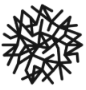
\includegraphics[width=0.2\textwidth]{imag/redes}
}
\clearpage
%___________________________________________________________________________________________
\section{Visualizaci\'on en R}
En este apartado recae todo el peso del trabajo. \'Este se centra en ver qu\'e diagramas se pueden implementar con las funciones que prove\'e el lenguaje R combinado con los dem\'as paquetes.~\\
Con cada diagrama se intenta buscar m\'as de una manera de crearlos con diferentes paquetes, y poder establecer, diferentes formas de implementar dicho diagrama para posibles usos diferenciados de este.~\\
En las siguientes subsecciones se expondr\'an los diagramas circulares que se han podido implementar con el lenguaje R.
\subsection{Diagrama de Anillos}\label{ssec:anillos}
Este diagrama consiste en un grupo de c\'irculos conc\'entricos. En cada uno de ellos se puede representar: una informaci\'on diferente con diferentes gr\'aficos o, la misma informaci\'on con mismos tipos de gr\'aficos solo que con una variable diferente para poder realizar comparaciones.
\subsubsection{Paquete ggplot2}
Se empieza con uno de los paquetes que m\'as ser\'a usado a lo largo del trabajo\cite{docu_ggplot2}
, debido a que es uno de los m\'as vers\'atiles y personalizables, pues se puede retocar y ajustar cada uno de los componentes del gr\'afico que resulte de este; como la escala, el sistema de coordenadas, la etiquetas, etc.
Tambi\'en, una de las mejores caracteristicas de este paquete, es su compatibilidad con otros paquetes de modificaci\'on de datos o de realizaci\'on de gr\'aficos.~\\
Lo primero que se va a necesitar en todas las demostraciones de este trabajo es la obtenci\'on y manipulaci\'on de los datos. En este caso se necesitan 2 variables, indicando cuantos anillos componen el diagrama y el ancho de cada uno de ellos.~\\
La primera forma de crear los anillos usa la funci\'on \texttt{geom-bar}, la cual reproduce el diagramas de barras cl\'asico, obteniendo su magnitud de la varible que se asigne para indicar su ancho.~\\Los datos que se van a usar son: una serie de entidades y sus valores porcentuales. En este caso se generan aleatoriamente, pero se pueden obtener como la frecuencia de los datos en una columna, de cualquier base de datos, proporcionando un valor porcentual a la frecuencia.
\begin{knitrout}
\definecolor{shadecolor}{rgb}{0.969, 0.969, 0.969}\color{fgcolor}\begin{kframe}
\begin{alltt}
\hlstd{datos} \hlkwb{<-} \hlkwd{data.frame}\hlstd{(}
  \hlkwc{anillos}\hlstd{=LETTERS[}\hlnum{1}\hlopt{:}\hlnum{10}\hlstd{],}
  \hlkwc{ancho}\hlstd{=}\hlkwd{c}\hlstd{(}\hlnum{10}\hlstd{,}\hlnum{8}\hlstd{,}\hlnum{10}\hlstd{,}\hlnum{9}\hlstd{,}\hlnum{5}\hlstd{,}\hlnum{12}\hlstd{,}\hlnum{20}\hlstd{,}\hlnum{6}\hlstd{,}\hlnum{10}\hlstd{,}\hlnum{10}\hlstd{)}
\hlstd{)}
\end{alltt}
\end{kframe}
\end{knitrout}
En esta prueba se establecen 10 anillos designados por letras, como el nombre de entidades, y el ancho de cada uno es el valor porcentual.

Lo primero ser\'a cargar la librer\'ia ggplot2 para poder usar sus funciones.
\begin{knitrout}
\definecolor{shadecolor}{rgb}{0.969, 0.969, 0.969}\color{fgcolor}\begin{kframe}
\begin{alltt}
\hlkwd{library}\hlstd{(ggplot2)}
\end{alltt}
\end{kframe}
\end{knitrout}
Para empezar con la funci\'on principal del paquete, es necesario indicar la fuente de sus datos y qu\'e cargar en cada variable. El eje X indicar\'a qu\'e significa cada anillo, para este ejemplo, se deja vac\'io. Al eje Y se le asigna el ancho de los anillos y, para colorear cada anillo independientemente, se usa la variable fill (rellenar).
\begin{knitrout}
\definecolor{shadecolor}{rgb}{0.969, 0.969, 0.969}\color{fgcolor}\begin{kframe}
\begin{alltt}
\hlkwd{ggplot}(datos, \hlkwd{aes}(x=\hlstr{""}, y=ancho, fill=anillos)) +
\end{alltt}
\end{kframe}
\end{knitrout}
Una vez establecidos los par\'ametros iniciales se procede a usar la funci\'on para implementar en la plantilla, y, c\'omo se van a usar barras, el paquete ofrece la funci\'on \texttt{geom-bar}. Para este ejemplo, se va a diferenciar cada uno de los valores de Y para una barra (stat = identity) y se establece el ancho al 100\% de su valor y el color de los bordes de cada anillo es gris.
\begin{knitrout}
\definecolor{shadecolor}{rgb}{0.969, 0.969, 0.969}\color{fgcolor}\begin{kframe}
\begin{alltt}
  \hlkwd{geom_bar}(stat=\hlstr{"identity"}, width=1, colour=\hlstr{"grey90"}) +
\end{alltt}
\end{kframe}
\end{knitrout}
\clearpage
Ahora no es mas que un diagrama de barras tradicional, donde las barras tienen la misma longitud, asi que, para hacer que las barras se conviertan en anillos, es necesario cambiar su sistema de coordenadas de cartesianas a polares, con la funci\'on \texttt{coord-polar}. Por defecto se establece que la primera variable con datos sea la que se cambia de sistema de coordenadas, en este caso el eje Y.
\begin{knitrout}
\definecolor{shadecolor}{rgb}{0.969, 0.969, 0.969}\color{fgcolor}\begin{kframe}
\begin{alltt}
  \hlkwd{coord_polar}() +
\end{alltt}
\end{kframe}
\end{knitrout}
Por \'ultimo, se usan unas funciones para alterar el tema del gr\'afico como el fondo, la cuadr\'icula, la leyenda, etc. Pero, para este ejemplo, se prefiere carecer de todo ello para una mejor est\'etica.
\begin{knitrout}
\definecolor{shadecolor}{rgb}{0.969, 0.969, 0.969}\color{fgcolor}\begin{kframe}
\begin{alltt}
  \hlkwd{theme_void}\hlstd{()} \hlopt{+}
  \hlkwd{theme}\hlstd{(}\hlkwc{legend.position}\hlstd{=}\hlstr{"none"}\hlstd{)}
\end{alltt}
\end{kframe}
\end{knitrout}
Resultando en:
\begin{knitrout}
\definecolor{shadecolor}{rgb}{0.969, 0.969, 0.969}\color{fgcolor}

{\centering 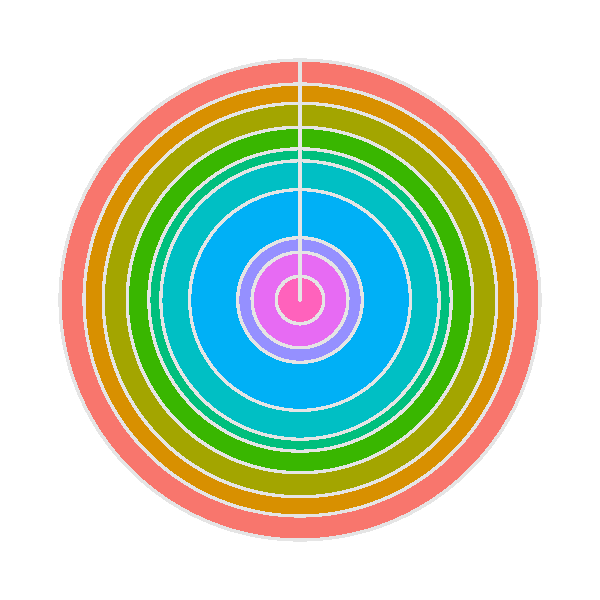
\includegraphics[width=\maxwidth]{figure/plot_ring_gg1-1} 

}



\end{knitrout}

\clearpage
Otras de las funciones que pueden imitar al \texttt{geom-bar} son: \texttt{geom-col, geom-tile}. Para cada una de ellas, es necesario una aproximaci\'on diferente; \texttt{geom-col} es muy similar a bar solo que no hace falta el argumento stat=identity.
La funci\'on \texttt{geom-tile} sirve para crear rect\'angulos y, para delimitarlos, no sirven los mismos datos que antes, ya que esto solo se pueden crear anillos con mismo valor, por ejemplo 1. Con esta funci\'on se puede representar la variedad de entidades que existen, por ejemplo, los diferentes valores en una columna de cualquier base de datos. Esta vez se utiliza el eje X para los anillos y, como antes, el eje Y para el ancho. Esta vez hay que especificar qu\'e variable se transforma a coordenadas polares aunque, por lo dem\'as, es lo mismo salvo que se experimenta a no colorear los bordes de los rect\'angulos.
\begin{knitrout}
\definecolor{shadecolor}{rgb}{0.969, 0.969, 0.969}\color{fgcolor}\begin{kframe}
\begin{alltt}
\hlstd{datos} \hlkwb{<-} \hlkwd{data.frame}\hlstd{(}
  \hlkwc{anillos}\hlstd{=LETTERS[}\hlnum{1}\hlopt{:}\hlnum{10}\hlstd{],}
  \hlkwc{ancho}\hlstd{=}\hlkwd{c}\hlstd{(}\hlkwd{rep}\hlstd{(}\hlnum{1}\hlstd{,}\hlnum{10}\hlstd{))}
\hlstd{)}
\hlkwd{ggplot}\hlstd{(datos,} \hlkwd{aes}\hlstd{(}\hlkwc{x}\hlstd{=anillos,} \hlkwc{y}\hlstd{=ancho))} \hlopt{+}
  \hlkwd{geom_tile}\hlstd{(}\hlkwd{aes}\hlstd{(}\hlkwc{fill} \hlstd{= anillos))} \hlopt{+}
  \hlkwd{coord_polar}\hlstd{(}\hlstr{'y'}\hlstd{)} \hlopt{+}
  \hlkwd{theme_void}\hlstd{()}
\end{alltt}
\end{kframe}

{\centering 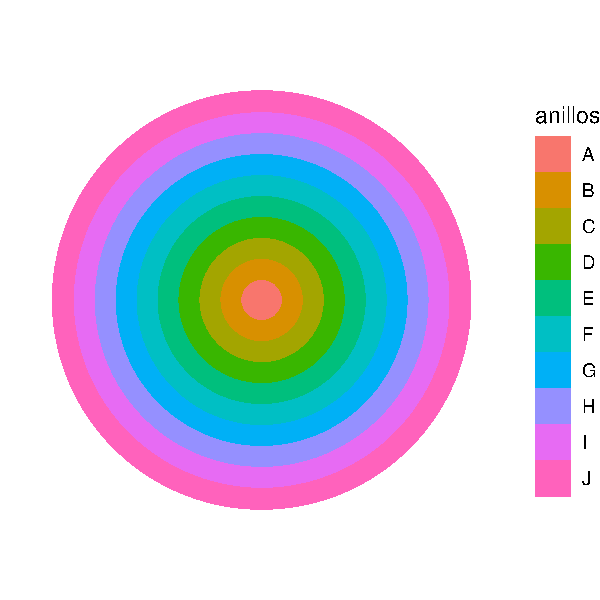
\includegraphics[width=\maxwidth]{figure/plot_ring_gg2-1} 

}



\end{knitrout}
\clearpage
\subsubsection{Paquete circlize}
Este es otro de los paquetes m\'as versatiles para los gr\'aficos con dise\~no circular\cite{docu_circlize}
. Al contrario que ggplot2 que crea gr\'aficos y necesita cambiarlos de sistemas de coordenadas, este paquete ya esta dise\~nado para diagramas circulares.~\\
Lo primero que se necesita hacer es establecer que no se divida cada anillo, ya que circlize permite la posibilidad de dividirlos generando una cuadr\'icula circular.
\begin{knitrout}
\definecolor{shadecolor}{rgb}{0.969, 0.969, 0.969}\color{fgcolor}\begin{kframe}
\begin{alltt}
\hlstd{datos} \hlkwb{<-} \hlkwd{data.frame}\hlstd{(}
  \hlkwc{division} \hlstd{=} \hlkwd{sample}\hlstd{(letters[}\hlnum{1}\hlstd{],} \hlnum{1000}\hlstd{,} \hlkwc{replace} \hlstd{=} \hlnum{TRUE}\hlstd{),}
  \hlkwc{x} \hlstd{=} \hlkwd{runif}\hlstd{(}\hlnum{1000}\hlstd{)}\hlopt{*}\hlnum{10}\hlstd{,}
  \hlkwc{y} \hlstd{=} \hlkwd{runif}\hlstd{(}\hlnum{1000}\hlstd{)}
\hlstd{)}
\end{alltt}
\end{kframe}
\end{knitrout}

La variable divisi\'on establece que cada anillo solo tendr\'a un vector con 1000 datos y las otras dos variables se van a usar en los diferentes diagramas de cada anillo. Representando la variable X e Y de los gr\'aficos l\'ineas y puntos. Para la parte del histograma s\'olo se requiere de una variable de los datos, mostrando la frecuencia de los valores de la variable entre intervalos. ~\\~\\
Se necesita crear una plantilla para cada diagrama. Esta se genera primero al inicializar el gr\'afico y luego con las funciones \texttt{trackPlotRegion} o \texttt{track} para realizar las plantillas de cada anillo.
\begin{knitrout}
\definecolor{shadecolor}{rgb}{0.969, 0.969, 0.969}\color{fgcolor}\begin{kframe}
\begin{alltt}
\hlkwd{library}\hlstd{(circlize)}
\hlkwd{circos.par}\hlstd{(}\hlstr{"track.height"} \hlstd{=} \hlnum{0.22}\hlstd{)}
\hlkwd{circos.initialize}\hlstd{(} \hlkwc{factors}\hlstd{=datos}\hlopt{$}\hlstd{division,} \hlkwc{x}\hlstd{=datos}\hlopt{$}\hlstd{x)}
\end{alltt}
\end{kframe}
\end{knitrout}
Con la funci\'on \texttt{trackPlotRegion} se crea la plantilla con la altura que establece la escala de la variable Y, junto con la leyenda del eje X, por fuera del c\'irculo (por defecto).
\begin{knitrout}
\definecolor{shadecolor}{rgb}{0.969, 0.969, 0.969}\color{fgcolor}\begin{kframe}
\begin{alltt}
\hlkwd{circos.trackPlotRegion}\hlstd{(}\hlkwc{factors} \hlstd{= datos}\hlopt{$}\hlstd{division,} \hlkwc{y} \hlstd{= datos}\hlopt{$}\hlstd{y,} \hlkwc{panel.fun} \hlstd{=} \hlkwa{function}\hlstd{(}\hlkwc{x}\hlstd{,} \hlkwc{y}\hlstd{) \{}
  \hlkwd{circos.axis}\hlstd{()\})}
\end{alltt}
\end{kframe}
\end{knitrout}
Para recrear los diferentes gr\'aficos, se van a usar 3 m\'etodos diferentes. El primero consiste en crear el gr\'afico de l\'ineas despu\'es de crear la plantilla.
\begin{knitrout}
\definecolor{shadecolor}{rgb}{0.969, 0.969, 0.969}\color{fgcolor}\begin{kframe}
\begin{alltt}
\hlkwd{circos.trackLines}\hlstd{(datos}\hlopt{$}\hlstd{division, datos}\hlopt{$}\hlstd{x[}\hlkwd{order}\hlstd{(datos}\hlopt{$}\hlstd{x)], datos}\hlopt{$}\hlstd{y[}\hlkwd{order}\hlstd{(datos}\hlopt{$}\hlstd{x)],}
                  \hlkwc{col} \hlstd{=} \hlkwd{rgb}\hlstd{(}\hlnum{0.1}\hlstd{,}\hlnum{0.5}\hlstd{,}\hlnum{0.8}\hlstd{,}\hlnum{0.3}\hlstd{),} \hlkwc{lwd}\hlstd{=}\hlnum{2}\hlstd{)}
\end{alltt}
\end{kframe}
\end{knitrout}
El segundo m\'etodo se da cuando una de las funciones ya crea la plantilla; como \texttt{trackHist}.
\begin{knitrout}
\definecolor{shadecolor}{rgb}{0.969, 0.969, 0.969}\color{fgcolor}\begin{kframe}
\begin{alltt}
\hlkwd{circos.trackHist}\hlstd{(datos}\hlopt{$}\hlstd{division, datos}\hlopt{$}\hlstd{x[}\hlkwd{order}\hlstd{(datos}\hlopt{$}\hlstd{x)],} \hlkwc{col} \hlstd{=} \hlkwd{rgb}\hlstd{(}\hlnum{0.1}\hlstd{,}\hlnum{0.5}\hlstd{,}\hlnum{0.8}\hlstd{,}\hlnum{0.3}\hlstd{),} \hlkwc{lwd}\hlstd{=}\hlnum{2}\hlstd{)}
\end{alltt}
\end{kframe}
\end{knitrout}
Por \'ultimo, el tercer m\'etodo consiste en crear la plantilla con \texttt{track} y dentro de esta se incluye la funci\'on que realiza el gr\'afico.
\begin{knitrout}
\definecolor{shadecolor}{rgb}{0.969, 0.969, 0.969}\color{fgcolor}\begin{kframe}
\begin{alltt}
\hlkwd{circos.track}\hlstd{(datos}\hlopt{$}\hlstd{division,} \hlkwc{x} \hlstd{= datos}\hlopt{$}\hlstd{x[}\hlkwd{order}\hlstd{(datos}\hlopt{$}\hlstd{x)],} \hlkwc{y} \hlstd{= datos}\hlopt{$}\hlstd{y[}\hlkwd{order}\hlstd{(datos}\hlopt{$}\hlstd{x)],}
             \hlkwc{panel.fun} \hlstd{=} \hlkwa{function}\hlstd{(}\hlkwc{x}\hlstd{,} \hlkwc{y}\hlstd{) \{}
               \hlkwd{circos.points}\hlstd{(x, y,} \hlkwc{pch} \hlstd{=} \hlnum{16}\hlstd{,} \hlkwc{cex} \hlstd{=} \hlnum{0.5}\hlstd{)\})}
\end{alltt}
\end{kframe}
\end{knitrout}
Todas las funciones usadas se pueden realizar con los tres m\'etodos, ya que existe la funci\'on para usar sin la funci\'on \texttt{track} y la que se usa dentro de ella.~\\
Al final se vuelve a representar el eje X para mejor visualizaci\'on. Y se emplea \texttt{circos.clear} para limpiar las variables, para que al volver a crear con circlize todas sus variables no esten modificadas.
\begin{knitrout}
\definecolor{shadecolor}{rgb}{0.969, 0.969, 0.969}\color{fgcolor}\begin{kframe}
\begin{alltt}
\hlkwd{circos.axis}\hlstd{(}\hlkwc{h}\hlstd{=}\hlstr{"bottom"}\hlstd{,}\hlkwc{direction} \hlstd{=} \hlstr{"inside"}\hlstd{,} \hlkwc{labels.facing}\hlstd{=} \hlstr{"clockwise"}\hlstd{,} \hlkwc{labels.cex} \hlstd{=} \hlnum{0.5}\hlstd{)}
\hlkwd{circos.clear}\hlstd{()}
\end{alltt}
\end{kframe}
\end{knitrout}
\clearpage
Resultando en el siguiente gr\'afico:~\\~\\
\begin{knitrout}
\definecolor{shadecolor}{rgb}{0.969, 0.969, 0.969}\color{fgcolor}

{\centering 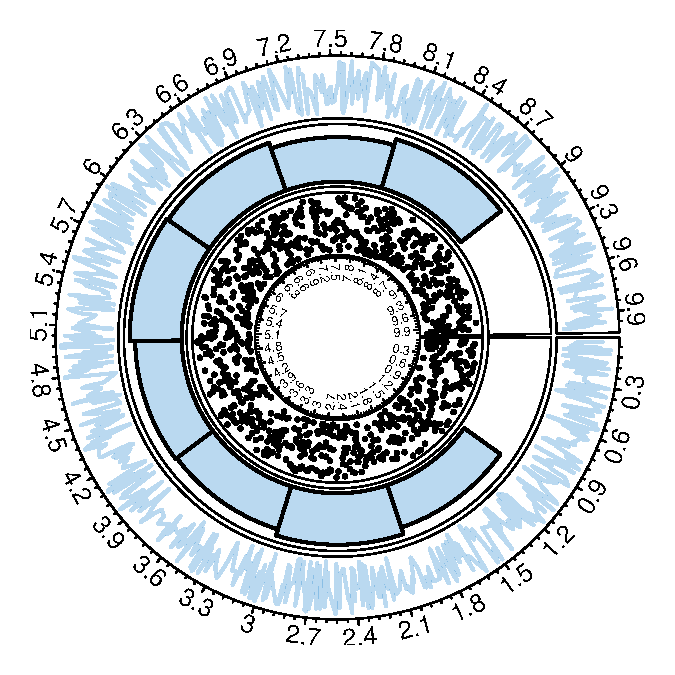
\includegraphics[width=\maxwidth]{figure/plot_ring_cir-1} 

}



\end{knitrout}
\begin{center}
\textbf{. . .}
\end{center}
\subsubsection{Paquete CMplot}
Este paquete se sustenta en el diagrama Manhattan convirti\'endolo en una variable circular del Manhattan\cite{docu_CMplot}
. Este es un tipo de diagrama de dispersi\'on, generalmente usado para representar datos con una gran cantidad de puntos y con una distribuci\'on de valores de gran magnitud.~\\
Este diagrama se usa mucho para representar estudios de genoma, situando en el eje X la posici\'on del cromosoma y en el eje Y el rango de asociaci\'on con un rasgo.~\\
Para el ejemplo con este paquete, se va a hacer uso de uno de los datos que proporciona el propio paquete \texttt{pig60k}, el cual da los resultados de asociaci\'on de todo el genoma de 3 rasgos, cuyos individuos fueron genotipados por chip de cerdo 60k.
\begin{knitrout}
\definecolor{shadecolor}{rgb}{0.969, 0.969, 0.969}\color{fgcolor}\begin{kframe}
\begin{alltt}
\hlkwd{library}\hlstd{(CMplot)}
\hlkwd{data}\hlstd{(pig60K)}
\end{alltt}
\end{kframe}
\end{knitrout}
\clearpage
Ahora se entra en detalle de la funci\'on principal del paquete \texttt{CMplot}.

Los primeros argumentos consisten: en los datos que se van a usar, el tipo de diagrama (en este caso de puntos), el dise\~no del diagrama (circular), el radio, el color para los puntos y las etiquetas.
\begin{knitrout}
\definecolor{shadecolor}{rgb}{0.969, 0.969, 0.969}\color{fgcolor}\begin{kframe}
\begin{alltt}
\hlkwd{CMplot}(pig60K,type=\hlstr{"p"},plot.type=\hlstr{"c"},r=0.4,col=\hlkwd{c}(\hlstr{"grey30"},\hlstr{"grey60"})
       ,chr.labels=\hlkwd{paste}(\hlstr{"Chr"},\hlkwd{c}(1:18,\hlstr{"X"}),sep=\hlstr{""}),
\end{alltt}
\end{kframe}
\end{knitrout}
Se establece el umbral, el ancho para el l\'imite, la amplificaci\'on de los puntos significativos, el tipo de l\'inea y color para el umbral.
\begin{knitrout}
\definecolor{shadecolor}{rgb}{0.969, 0.969, 0.969}\color{fgcolor}\begin{kframe}
\begin{alltt}
      threshold=\hlkwd{c}(1e-6,1e-4),cir.chr.h=1.5,amplify=TRUE,threshold.lty=\hlkwd{c}(1,2)
      ,threshold.col=\hlkwd{c}(\hlstr{"red"},\hlstr{"blue"})
\end{alltt}
\end{kframe}
\end{knitrout}
El ancho de la l\'inea se establece con los SNPs significativos, su color, el color para la densidad SNP.
\begin{knitrout}
\definecolor{shadecolor}{rgb}{0.969, 0.969, 0.969}\color{fgcolor}\begin{kframe}
\begin{alltt}
      ,signal.line=1,signal.col=\hlkwd{c}(\hlstr{"red"},\hlstr{"green"}),chr.den.col=\hlkwd{c}(\hlstr{"darkgreen"},\hlstr{"yellow"},\hlstr{"red"}),
\end{alltt}
\end{kframe}
\end{knitrout}
El tama\~no de bin para el gr\'afico de densidad SNP, se exponen los puntos de exterior hacia interior, el tipo de fichero que genera y la resoluci\'on de la imagen.
\begin{knitrout}
\definecolor{shadecolor}{rgb}{0.969, 0.969, 0.969}\color{fgcolor}\begin{kframe}
\begin{alltt}
      bin.size=1e6,outward=FALSE,file=\hlstr{"jpg"},dpi=300
      ,file.output=TRUE,verbose=TRUE,width=10,height=10)
\end{alltt}
\end{kframe}
\end{knitrout}
Dando un resultado de:~\\
\vbox{
    \centering
    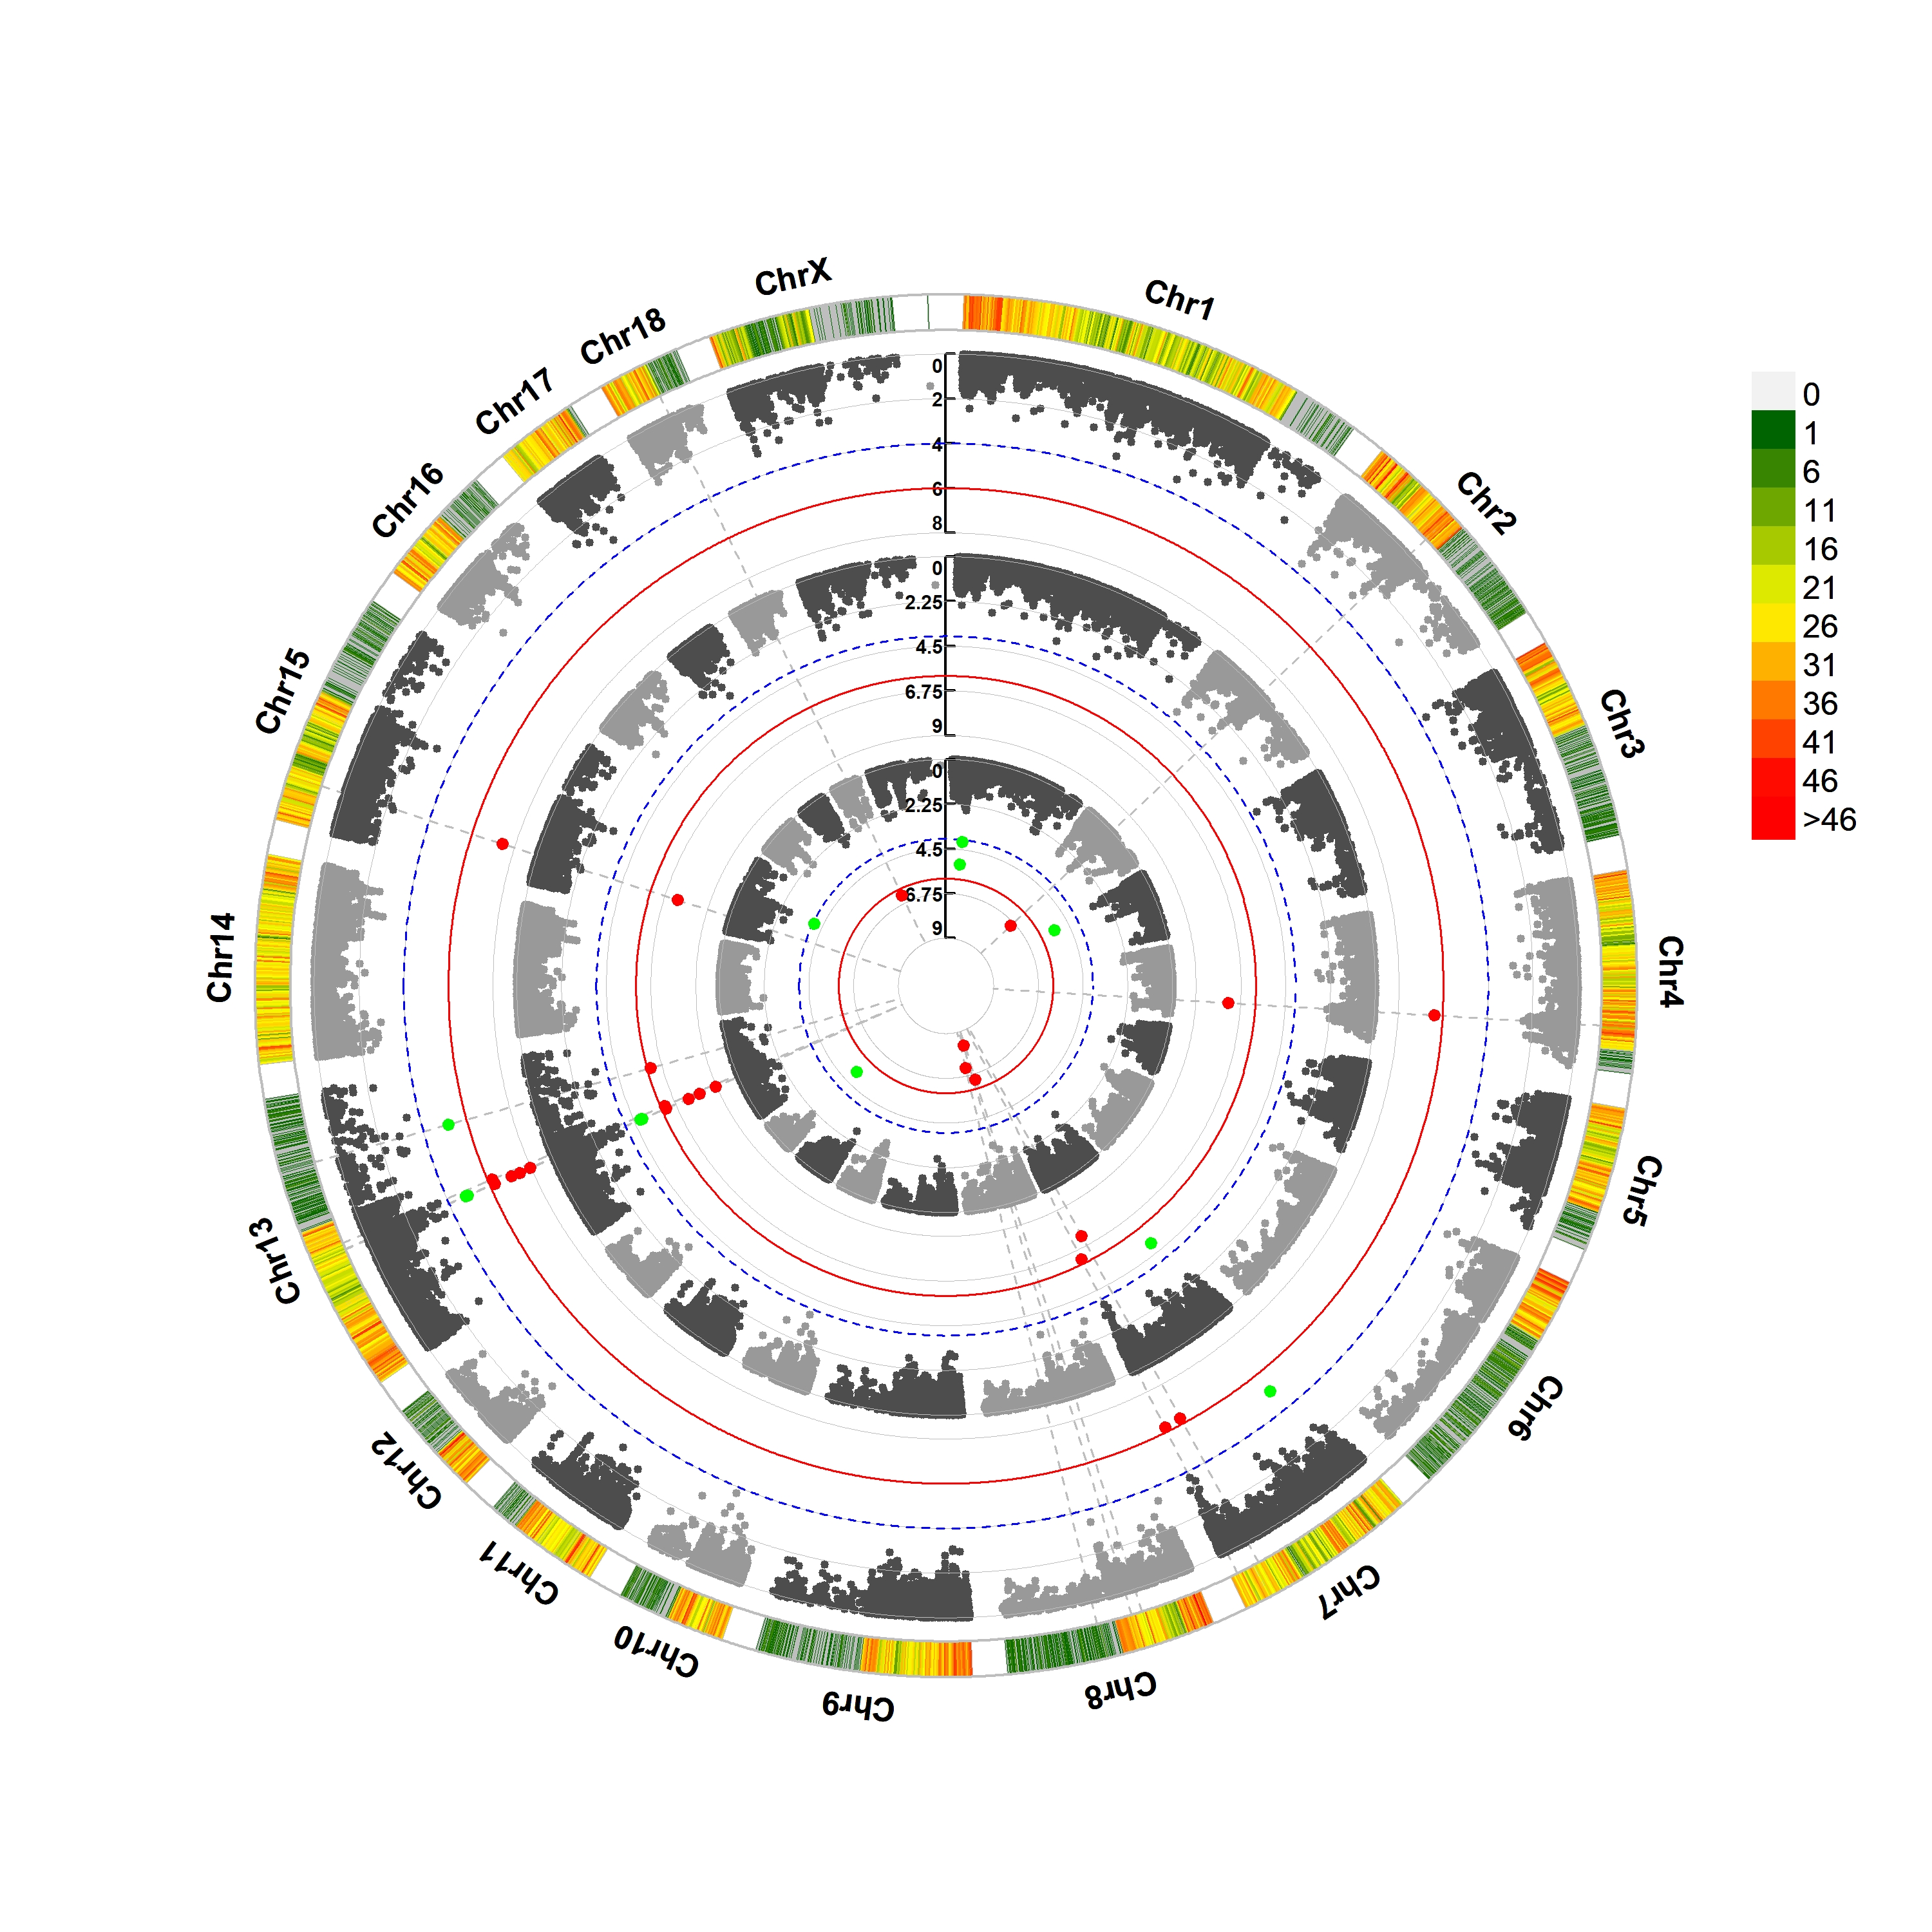
\includegraphics[width=0.6\textwidth]{imag/CMplot}
}
\clearpage
\subsubsection{Comparaciones}
En este apartado, que se va a repetir en todos los diagramas que se han podido implementar con alg\'un paquete de R, sirve para visualizar las diferencias o similitudes entre paquetes, en lo que respecta al resultado obtenido.~\\
Para realizar este diagrama se han utilizado 3 paquetes:~\\ 
El primero es el \texttt{ggplot2}, que implementa el diagrama de anillos utilizando de base un diagrama de barras tradicional (con sistema de coordenadas cartesianas), por lo que, en este sentido, el paquete est\'a limitado y no ofrezce otras variantes del diagrama de anillos, aunque, en cuanto a personalizaci\'on se comprueba que se puede modificar cualquier parte est\'etica del gr\'afico.~\\
El segundo paquete es \texttt{circlize}, que al estar basado directamente en gr\'aficos circulares, no necesita un cambio de sistema de coordenadas, y ofrece gran cantidad de gr\'aficos para cada uno de los anillos. En ese sentido, es el mejor de los tres paquetes presentados.Y, en personalizaci\'on, este paquete no se queda atras debido a que tambi\'en se puede retocar cualquier parte del diagrama.~\\
Y por \'ultimo, el tercer paquete es \texttt{CMplot}, consiste en una variante con dise\~no circular del paquete \texttt{qqman}, el cual, como se ha explicado antes, es un diagrama de Manhattan, por lo que este paquete esta limitado como ggplot2 a un solo tipo de diagrama para los anillos. Dentro del gr\'afico se pueden personalizar muchos aspectos del mismo.~\\
En conclusi\'on; el paquete m\'as versatil a la hora de este diagrama es \texttt{circlize}, debido a que, con cada uno de sus gr\'aficos, podr\'ia replicar los resultados de los otros dos. Para implementar gr\'aficos de genomas el paquete \texttt{CMplot} es m\'as facil de realizar que si se intenta imitar con circlize.
%%%%%%%%%%%%%%%%%%%%%%%%%%%%%%%%%%%%%%%%%%%%%%%%%%%%%%
\clearpage
%%%%%%%%%%%%%%%%%%%%%%%%%%%%%%%%%%%%%%%%%%%%%%%%%%%%%%%%%%%%%%%%%%
\subsection{Diagrama de Barras Radiales} \label{ssec:barrasRadiales}
Hay varias formas de aproximarse para realizar este tipo de diagramas, una de ellas consiste en realizar un diagrama de barras tradicional y convertir su eje Y al formato radial, la otra forma, se realiza creando un c\'irculo como plantilla y arcos como las barras (c\'irculos conc\'entricos).~\\
En este apartado se encuentran un paquete para la primera f\'ormula y dos para la segunda, pero todos los paquetes dan un gr\'afico muy similar. Aunque unos dan m\'as  posiblilidades de personalizaci\'on, son m\'as complejos.
\subsubsection{Paquete ggplot2}
En el punto anterior ya se ha visto este paquete\cite{docu_ggplot2}
 y, durante todos los dem\'as puntos, se demostrar\'a lo vers\'atil que es. En este tipo de grafo, lo que hay que hacer es un buen diagrama de barras tradicional con este paquete y aplicarle la coordenada polar, la cual transforma la coordenada deseada de formato lineal a circular.~\\
Primero se crea la tabla con el nombre de las barras y su valor, en este caso la importancia de Internet que tienen las categorias al tomar decisiones. Y se carga la libreria para despu\'es usar sus funciones:

\begin{knitrout}
\definecolor{shadecolor}{rgb}{0.969, 0.969, 0.969}\color{fgcolor}\begin{kframe}
\begin{alltt}
\hlkwd{library}\hlstd{(ggplot2)}
\hlstd{Category} \hlkwb{<-} \hlkwd{c}\hlstd{(}\hlstr{"Electronics"}\hlstd{,} \hlstr{"Appliances"}\hlstd{,} \hlstr{"Books"}\hlstd{,} \hlstr{"Music"}\hlstd{,} \hlstr{"Clothing"}\hlstd{,}
              \hlstr{"Cars"}\hlstd{,} \hlstr{"Food"}\hlstd{,} \hlstr{"Hygiene"}\hlstd{,}
              \hlstr{"Health/OTC"}\hlstd{,} \hlstr{"Hair Care"}\hlstd{)}
\hlstd{Percent} \hlkwb{<-} \hlkwd{c}\hlstd{(}\hlnum{81}\hlstd{,} \hlnum{77}\hlstd{,} \hlnum{70}\hlstd{,} \hlnum{69}\hlstd{,} \hlnum{69}\hlstd{,} \hlnum{68}\hlstd{,} \hlnum{62}\hlstd{,} \hlnum{62}\hlstd{,} \hlnum{61}\hlstd{,} \hlnum{60}\hlstd{)}
\hlstd{internetImportance}\hlkwb{<-}\hlkwd{data.frame}\hlstd{(Category,Percent)}
\end{alltt}
\end{kframe}
\end{knitrout}
Se transforma los nombres de las barras para que cuando se escriban se adhiera los valores a los nombres.
\begin{knitrout}
\definecolor{shadecolor}{rgb}{0.969, 0.969, 0.969}\color{fgcolor}\begin{kframe}
\begin{alltt}
\hlstd{internetImportance}\hlopt{$}\hlstd{Category} \hlkwb{<-}
  \hlkwd{paste0}\hlstd{(internetImportance}\hlopt{$}\hlstd{Category,}\hlstr{" - "}\hlstd{,internetImportance}\hlopt{$}\hlstd{Percent,}\hlstr{"%"}\hlstd{)}
\end{alltt}
\end{kframe}
\end{knitrout}
Y se ordenan, de mayor a menor, por como trabaja la libreria al crear el diagrama de exterior hacia el interior.
\begin{knitrout}
\definecolor{shadecolor}{rgb}{0.969, 0.969, 0.969}\color{fgcolor}\begin{kframe}
\begin{alltt}
\hlstd{internetImportance}\hlopt{$}\hlstd{Category} \hlkwb{<-}
  \hlkwd{factor}\hlstd{(internetImportance}\hlopt{$}\hlstd{Category,}
         \hlkwc{levels}\hlstd{=}\hlkwd{rev}\hlstd{(internetImportance}\hlopt{$}\hlstd{Category))}
\end{alltt}
\end{kframe}
\end{knitrout}
Y, despu\'es de esto, se realiza el plot del diagrama circular.

Gracias a esta funci\'on se prepara el espacio para recrear el gr\'afico con los par\'ametros b\'asicos de los datos y la est\'etica del gr\'afico. Las categor\'ias se representan en el eje X y el porcentaje en el eje Y, rellenando la figura geom\'etrica que quiera representar, en funci\'on de las categor\'ias.
\begin{knitrout}
\definecolor{shadecolor}{rgb}{0.969, 0.969, 0.969}\color{fgcolor}\begin{kframe}
\begin{alltt}
\hlkwd{ggplot}(internetImportance, \hlkwd{aes}(x = Category, y = Percent,
                               fill = Category)) +
\end{alltt}
\end{kframe}
\end{knitrout}
Se va a elegir la figura geom\'etrica de la barra para representar el gr\'afico que, por ahora, est\'a en formato lineal.
\begin{knitrout}
\definecolor{shadecolor}{rgb}{0.969, 0.969, 0.969}\color{fgcolor}\begin{kframe}
\begin{alltt}
  \hlkwd{geom_bar}(width = 0.9, stat=\hlstr{"identity"})  + 
\end{alltt}
\end{kframe}
\end{knitrout}
Despu\'es se transforma el eje Y del formato lineal al formato radial.
\begin{knitrout}
\definecolor{shadecolor}{rgb}{0.969, 0.969, 0.969}\color{fgcolor}\begin{kframe}
\begin{alltt}
  \hlkwd{coord_polar}(theta = \hlstr{"y"}) +
\end{alltt}
\end{kframe}
\end{knitrout}
\clearpage
Para la est\'etica del gr\'afico se eliminan las etiquetas de los ejes. Y representando los 360 grados del c\'irculo al 100\% de los porcentajes.
\begin{knitrout}
\definecolor{shadecolor}{rgb}{0.969, 0.969, 0.969}\color{fgcolor}\begin{kframe}
\begin{alltt}
  \hlkwd{xlab}(\hlstr{""}) + \hlkwd{ylab}(\hlstr{""}) +
  \hlkwd{ylim}(\hlkwd{c}(0,100)) +
\end{alltt}
\end{kframe}
\end{knitrout}
Se establece el t\'itulo y el texto de las barras, eliminando el fondo y la leyenda del gr\'afico para mejor representaci\'on.
\begin{knitrout}
\definecolor{shadecolor}{rgb}{0.969, 0.969, 0.969}\color{fgcolor}\begin{kframe}
\begin{alltt}
  \hlkwd{ggtitle}\hlstd{(}\hlstr{"Categorias de Productos Influenciados por Internet"}\hlstd{)} \hlopt{+}
  \hlkwd{geom_text}\hlstd{(}\hlkwc{data} \hlstd{= internetImportance,} \hlkwc{hjust} \hlstd{=} \hlnum{1}\hlstd{,} \hlkwc{size} \hlstd{=} \hlnum{3}\hlstd{,}
            \hlkwd{aes}\hlstd{(}\hlkwc{x} \hlstd{= Category,} \hlkwc{y} \hlstd{=} \hlnum{0}\hlstd{,} \hlkwc{label} \hlstd{= Category,} \hlkwc{colour} \hlstd{= Category))} \hlopt{+}
  \hlkwd{theme_minimal}\hlstd{()} \hlopt{+}
  \hlkwd{theme}\hlstd{(}\hlkwc{legend.position} \hlstd{=} \hlstr{"none"}\hlstd{,}
        \hlkwc{panel.grid.major} \hlstd{=} \hlkwd{element_blank}\hlstd{(),}
        \hlkwc{panel.grid.minor} \hlstd{=} \hlkwd{element_blank}\hlstd{(),}
        \hlkwc{axis.line} \hlstd{=} \hlkwd{element_blank}\hlstd{(),}
        \hlkwc{axis.text.y} \hlstd{=} \hlkwd{element_blank}\hlstd{(),}
        \hlkwc{axis.text.x} \hlstd{=} \hlkwd{element_blank}\hlstd{(),}
        \hlkwc{axis.ticks} \hlstd{=} \hlkwd{element_blank}\hlstd{())}
\end{alltt}
\end{kframe}
\end{knitrout}
Y la figura queda como se ve a continuaci\'on.~\\~\\
\begin{knitrout}
\definecolor{shadecolor}{rgb}{0.969, 0.969, 0.969}\color{fgcolor}

{\centering 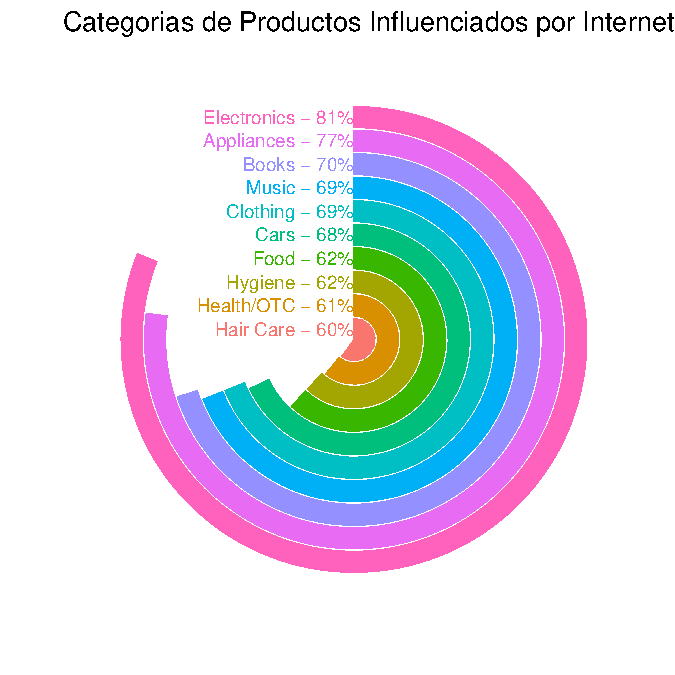
\includegraphics[width=\maxwidth]{figure/plot_ggp_cb-1} 

}



\end{knitrout}
\clearpage
Ahora se va a implementar uno de los grafos del libro\cite[p\'ag 76]{Circle}
, para ello se vuelven a preparar los datos como antes:

\begin{knitrout}
\definecolor{shadecolor}{rgb}{0.969, 0.969, 0.969}\color{fgcolor}\begin{kframe}
\begin{alltt}
\hlstd{Name} \hlkwb{<-} \hlkwd{rev}\hlstd{(}\hlkwd{c}\hlstd{(}\hlstr{"ANTIMONY"}\hlstd{,}\hlstr{"INDIUM"}\hlstd{,}\hlstr{"SILVER"}\hlstd{,}\hlstr{"COPPER"}\hlstd{,}\hlstr{"TITANIUM"}\hlstd{,}\hlstr{"TANTALUM"}\hlstd{,}\hlstr{"PHOSPHORUS"}\hlstd{,}
              \hlstr{"ALUMINIUM"}\hlstd{,}\hlstr{"GAS"}\hlstd{,}\hlstr{"OIL"}\hlstd{,}\hlstr{"COAL"}\hlstd{,}\hlstr{"AGRICUL. LAND"}\hlstd{,}\hlstr{"CORAL REEFS"}\hlstd{,} \hlstr{"RAINFOREST"}\hlstd{))}
\hlstd{Value} \hlkwb{<-} \hlkwd{rev}\hlstd{(}\hlkwd{c}\hlstd{(}\hlnum{8}\hlstd{,} \hlnum{12}\hlstd{,} \hlnum{17}\hlstd{,} \hlnum{32}\hlstd{,} \hlnum{44}\hlstd{,} \hlnum{46}\hlstd{,} \hlnum{76}\hlstd{,} \hlnum{80}\hlstd{,} \hlnum{35}\hlstd{,} \hlnum{37}\hlstd{,} \hlnum{42}\hlstd{,} \hlnum{69}\hlstd{,} \hlnum{88}\hlstd{,} \hlnum{100}\hlstd{))}
\hlstd{Group} \hlkwb{<-} \hlkwd{rev}\hlstd{(}\hlkwd{c}\hlstd{(}\hlstr{"minerals"}\hlstd{,}\hlstr{"minerals"}\hlstd{,}\hlstr{"minerals"}\hlstd{,}\hlstr{"minerals"}\hlstd{,}\hlstr{"minerals"}\hlstd{,}\hlstr{"minerals"}\hlstd{,}
           \hlstr{"minerals"}\hlstd{,}\hlstr{"minerals"}\hlstd{,}\hlstr{"fossil fuels"}\hlstd{,}\hlstr{"fossil fuels"}\hlstd{,}\hlstr{"fossil fuels"}\hlstd{,}
           \hlstr{"ecosystems"}\hlstd{,}\hlstr{"ecosystems"}\hlstd{,}\hlstr{"ecosystems"}\hlstd{))}
\hlstd{stockCheck}\hlkwb{<-}\hlkwd{data.frame}\hlstd{(Name,Value,Group)}
\hlcom{#Etiquetas}
\hlstd{stockCheck}\hlopt{$}\hlstd{Label} \hlkwb{<-} \hlkwd{paste0}\hlstd{(stockCheck}\hlopt{$}\hlstd{Name,}\hlstr{" "}\hlstd{)}
\end{alltt}
\end{kframe}
\end{knitrout}
Los datos representan la cantidad de a\~nos que tardan las categor\'ias en desaparecer.~\\
Para poder tener un espacio vacio en el centro hay que incluir varias lineas vacias, para que al implementarlas la funci\'on las borre, dejando el espacio en blanco
\begin{knitrout}
\definecolor{shadecolor}{rgb}{0.969, 0.969, 0.969}\color{fgcolor}\begin{kframe}
\begin{alltt}
\hlstd{len} \hlkwb{<-} \hlnum{5}
\hlstd{df2} \hlkwb{<-} \hlkwd{data.frame}\hlstd{(}\hlkwc{Name} \hlstd{= letters[}\hlnum{1}\hlopt{:}\hlstd{len],} \hlkwc{Value} \hlstd{=} \hlkwd{rep}\hlstd{(}\hlnum{NA}\hlstd{, len),}
                  \hlkwc{Group} \hlstd{=} \hlkwd{rep}\hlstd{(}\hlnum{NA}\hlstd{, len),} \hlkwc{Label} \hlstd{=} \hlkwd{rep}\hlstd{(}\hlstr{""}\hlstd{, len))}
\hlstd{stockCheck} \hlkwb{<-} \hlkwd{rbind}\hlstd{(stockCheck, df2)}
\hlcom{#ordenar por grupos}
\hlstd{stockCheck}\hlopt{$}\hlstd{Name} \hlkwb{<-} \hlkwd{factor}\hlstd{(stockCheck}\hlopt{$}\hlstd{Name,}
                          \hlkwc{levels} \hlstd{=} \hlkwd{rev}\hlstd{(stockCheck}\hlopt{$}\hlstd{Name[}\hlkwd{order}\hlstd{(stockCheck}\hlopt{$}\hlstd{Group)] ))}
\end{alltt}
\end{kframe}
\end{knitrout}
Y se realiza el grafo de la misma manera que la anterior, s\'olo que ahora, se deja espacio en el interior para que se visualice mejor el grafo.
Al ser de la misma forma que el anterior, se va a mostrar solo las opciones que este gr\'afico tenga de forma diferente.


Una de las diferencias con el anterior es la forma de crear el texto con el color seg\'un los grupos, y las etiquetas que se sit\'uan al final de las barras, siendo cuadrados rellenos con el color del grupo.
\begin{knitrout}
\definecolor{shadecolor}{rgb}{0.969, 0.969, 0.969}\color{fgcolor}\begin{kframe}
\begin{alltt}
  \hlkwd{geom_text}(data = stockCheck, hjust = 1, size = 3,
            \hlkwd{aes}(x = Name, y = 0, label = Label, colour = \hlkwd{factor}(Group), 
                fontface = \hlstr{"bold"})) +
  \hlkwd{geom_label}(\hlkwd{aes}(fill = \hlkwd{factor}(Group)), colour = \hlstr{"white"}) +
\end{alltt}
\end{kframe}
\end{knitrout}
Y se cambian los valores del color para asemejarlo al gr\'afico que se intenta implementar; tiene que ser 4 colores, debido a que hay un grupo de valores vac\'ios, para crear el hueco en el medio.
\begin{knitrout}
\definecolor{shadecolor}{rgb}{0.969, 0.969, 0.969}\color{fgcolor}\begin{kframe}
\begin{alltt}
  \hlkwd{scale_fill_manual}(values = \hlkwd{c}(\hlstr{"#edcf87"}, \hlstr{"#2c98db"},\hlstr{"#e83d31"},\hlstr{"#e83d31"} )) +
  \hlkwd{scale_color_manual}(values = \hlkwd{c}(\hlstr{"#edcf87"}, \hlstr{"#2c98db"},\hlstr{"#e83d31"},\hlstr{"#e83d31"} )) +
\end{alltt}
\end{kframe}
\end{knitrout}
\clearpage
Resultando en el siguiente gr\'afico.
\begin{knitrout}
\definecolor{shadecolor}{rgb}{0.969, 0.969, 0.969}\color{fgcolor}

{\centering 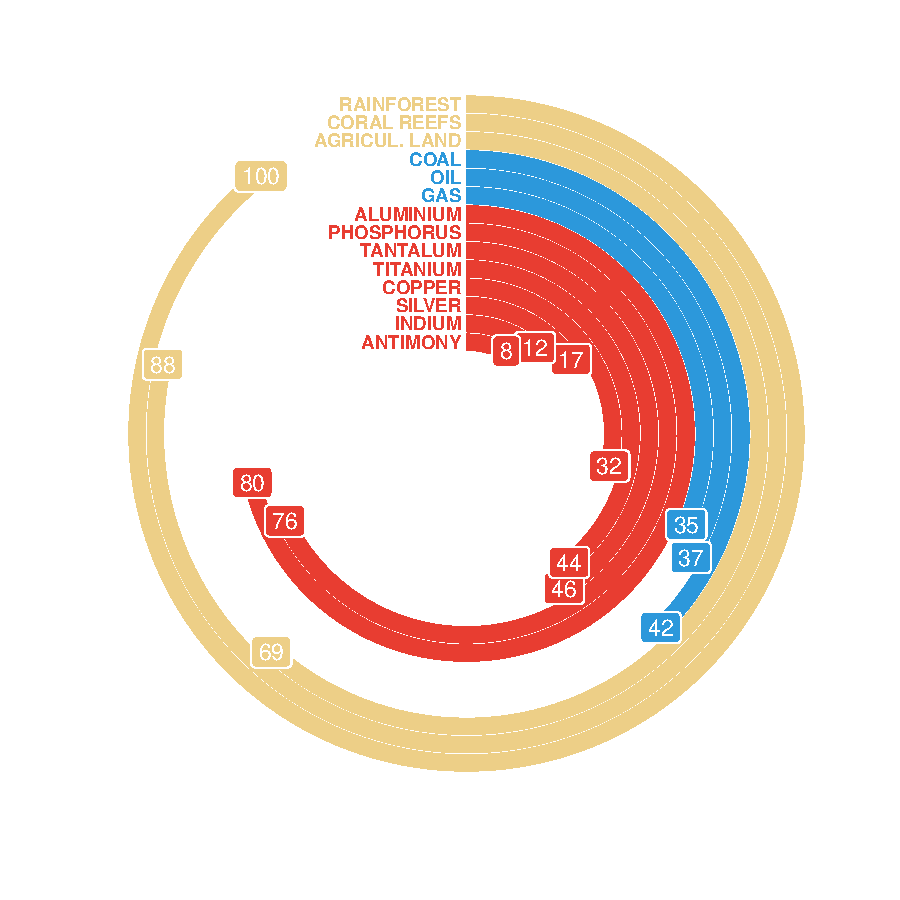
\includegraphics[width=\maxwidth]{figure/plot_br_final-1} 

}



\end{knitrout}
\begin{center}
\textbf{. . .}
\end{center}
~\\Existe un paquete que proporciona interactividad a los gr\'aficos del paquete ggplot2, y suele funcionar mejor cuando hay una gran cantidad de datos.~\\
El paquete \texttt{ggiraph}\cite{docu_ggiraph}
ayuda a crear la interactividad con algunas funciones que se unen al gr\'afico de ggplot2, en este caso, se usa \texttt{geom-col-interactive}, para crear las barras interactivas. Para que se represente bien hay que dar los valores aduacuados a las nuevas variables interactivas \texttt{tooltip} y \texttt{data-id}.~\\
Primero se necesita una gran cantidad de datos, aleatorios en este caso, creando los nombres de las entidades (barras) y sus valores.
\begin{knitrout}
\definecolor{shadecolor}{rgb}{0.969, 0.969, 0.969}\color{fgcolor}\begin{kframe}
\begin{alltt}
\hlstd{data} \hlkwb{<-} \hlkwd{data.frame}\hlstd{(}
  \hlkwc{id}\hlstd{=}\hlkwd{seq}\hlstd{(}\hlnum{1}\hlstd{,}\hlnum{30}\hlstd{),}
  \hlkwc{value}\hlstd{=}\hlkwd{sample}\hlstd{(} \hlkwd{seq}\hlstd{(}\hlnum{70}\hlstd{,}\hlnum{100}\hlstd{),} \hlnum{30}\hlstd{,} \hlkwc{replace}\hlstd{=T)}
\hlstd{)}
\hlstd{data}\hlopt{$}\hlstd{individual} \hlkwb{<-} \hlkwd{paste0}\hlstd{(} \hlstr{"Bar. "}\hlstd{, data}\hlopt{$}\hlstd{id,} \hlstr{"-"}\hlstd{, data}\hlopt{$}\hlstd{value,}\hlstr{"%"}\hlstd{)}
\end{alltt}
\end{kframe}
\end{knitrout}
\clearpage
Y ahora, asignar los par\'ametros adecuados al gr\'afico de ggplot2, con la funci\'on de columnas interactivas.
\begin{knitrout}
\definecolor{shadecolor}{rgb}{0.969, 0.969, 0.969}\color{fgcolor}\begin{kframe}
\begin{alltt}
\hlkwd{library}\hlstd{(ggiraph)}
\hlstd{p} \hlkwb{<-} \hlkwd{ggplot}\hlstd{(data,} \hlkwd{aes}\hlstd{(} \hlkwc{x} \hlstd{= individual,} \hlkwc{y} \hlstd{= value,} \hlkwc{tooltip} \hlstd{= individual,} \hlkwc{label} \hlstd{= value,}
                                     \hlkwc{data_id} \hlstd{= individual,} \hlkwc{fill} \hlstd{= individual) )} \hlopt{+}
  \hlkwd{geom_col_interactive}\hlstd{()} \hlopt{+}
  \hlkwd{coord_polar}\hlstd{(}\hlkwc{theta} \hlstd{=} \hlstr{'y'}\hlstd{)} \hlopt{+}
  \hlkwd{xlab}\hlstd{(}\hlstr{""}\hlstd{)} \hlopt{+} \hlkwd{ylab}\hlstd{(}\hlstr{""}\hlstd{)} \hlopt{+}
  \hlkwd{ylim}\hlstd{(}\hlkwd{c}\hlstd{(}\hlnum{0}\hlstd{,}\hlnum{101}\hlstd{))} \hlopt{+}
  \hlkwd{theme_minimal}\hlstd{()} \hlopt{+}
  \hlkwd{theme}\hlstd{(}\hlkwc{legend.position} \hlstd{=} \hlstr{"none"}\hlstd{,}
        \hlkwc{panel.grid.major} \hlstd{=} \hlkwd{element_blank}\hlstd{(),}
        \hlkwc{panel.grid.minor} \hlstd{=} \hlkwd{element_blank}\hlstd{(),}
        \hlkwc{axis.line} \hlstd{=} \hlkwd{element_blank}\hlstd{(),}
        \hlkwc{axis.text.y} \hlstd{=} \hlkwd{element_blank}\hlstd{(),}
        \hlkwc{axis.text.x} \hlstd{=} \hlkwd{element_blank}\hlstd{(),}
        \hlkwc{axis.ticks} \hlstd{=} \hlkwd{element_blank}\hlstd{())}
\end{alltt}
\end{kframe}
\end{knitrout}
Para la interactividad se necesita crear el objeto girafe (propio del paquete).
\begin{knitrout}
\definecolor{shadecolor}{rgb}{0.969, 0.969, 0.969}\color{fgcolor}\begin{kframe}
\begin{alltt}
\hlkwd{girafe}\hlstd{(}\hlkwc{ggobj} \hlstd{= p)}
\end{alltt}
\end{kframe}
\end{knitrout}
Dando como resultado el siguiente gr\'afico.~\\
\vbox{
    \centering
    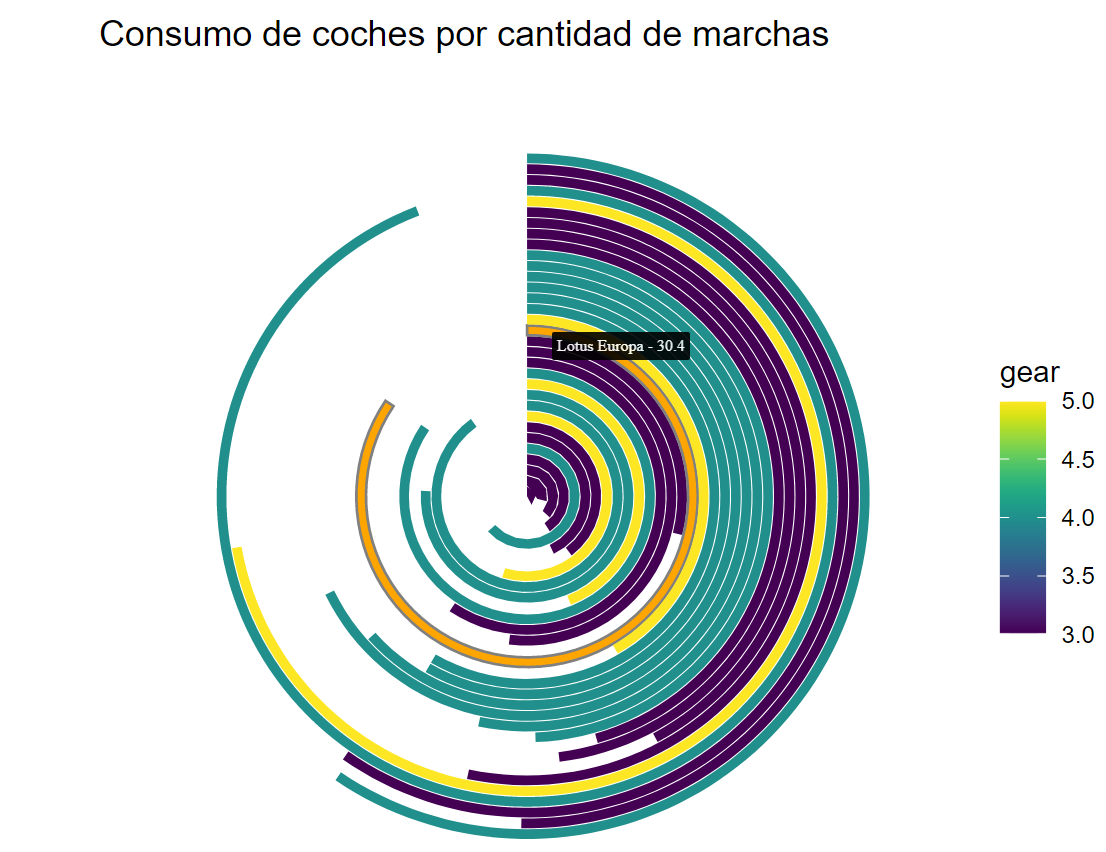
\includegraphics[width=0.5\textwidth]{imag/bar_interactive}
}
\clearpage
\subsubsection{Paquete Plotrix}
El paquete plotrix proporciona una serie de plots espec\'ificos que ofrecen una f\'acil personalizaci\'on (color, posici\'on del texto...).~\\
A lo largo del proyecto, se observar\'a dichos grafos utilizarse en los diferentes tipos de diagramas circulares.~\\
En la documentaci\'on \cite{docu_plotrix}
se encuentran los m\'etodos para crear este Diagrama de Barras Radiales, \texttt{draw.circle} y \texttt{draw.arc}, que se encargan de recrear los c\'irculos que se usaran de plantilla para que se expongan las barras. La orden \texttt{draw.arc} necesita conocer en cual \'angulo comienzan las barras y en cual terminan, adem\'as de los datos de las barras.

Primero llamar a la libreria.
\begin{knitrout}
\definecolor{shadecolor}{rgb}{0.969, 0.969, 0.969}\color{fgcolor}\begin{kframe}
\begin{alltt}
\hlkwd{library}\hlstd{(plotrix)}
\end{alltt}
\end{kframe}
\end{knitrout}
Luego se crea la funci\'on para crear el diagrama.
\begin{knitrout}
\definecolor{shadecolor}{rgb}{0.969, 0.969, 0.969}\color{fgcolor}\begin{kframe}
\begin{alltt}
circBarPlot <- \hlkwd{function}(x, labels, colors=\hlkwd{rainbow}(\hlkwd{length}(x)), cex.lab=1) \{
\end{alltt}
\end{kframe}
\end{knitrout}
Se establece el \'area para delimitar donde se realiza el c\'irculo.
\begin{knitrout}
\definecolor{shadecolor}{rgb}{0.969, 0.969, 0.969}\color{fgcolor}\begin{kframe}
\begin{alltt}
  \hlkwd{plot}\hlstd{(}\hlnum{0}\hlstd{,}\hlkwc{xlim}\hlstd{=}\hlkwd{c}\hlstd{(}\hlopt{-}\hlnum{1.2}\hlstd{,}\hlnum{1.2}\hlstd{),}\hlkwc{ylim}\hlstd{=}\hlkwd{c}\hlstd{(}\hlopt{-}\hlnum{1.2}\hlstd{,}\hlnum{1.2}\hlstd{),}\hlkwc{type}\hlstd{=}\hlstr{"n"}\hlstd{,}\hlkwc{axes}\hlstd{=F,} \hlkwc{xlab}\hlstd{=}\hlnum{NA}\hlstd{,} \hlkwc{ylab}\hlstd{=}\hlnum{NA}\hlstd{)}
\end{alltt}
\end{kframe}
\end{knitrout}
Se guardan los datos de las barras en una variable.
\begin{knitrout}
\definecolor{shadecolor}{rgb}{0.969, 0.969, 0.969}\color{fgcolor}\begin{kframe}
\begin{alltt}
  \hlstd{radii} \hlkwb{<-} \hlkwd{seq}\hlstd{(}\hlnum{1}\hlstd{,} \hlnum{0.3}\hlstd{,} \hlkwc{length.out}\hlstd{=}\hlkwd{length}\hlstd{(x))}
\end{alltt}
\end{kframe}
\end{knitrout}
Constituir la plantilla para los datos y el \'angulo de inicio del diagrama.
\begin{knitrout}
\definecolor{shadecolor}{rgb}{0.969, 0.969, 0.969}\color{fgcolor}\begin{kframe}
\begin{alltt}
  \hlkwd{draw.circle}\hlstd{(}\hlnum{0}\hlstd{,}\hlnum{0}\hlstd{,radii,}\hlkwc{border}\hlstd{=}\hlstr{"lightgrey"}\hlstd{)}
  \hlstd{angles} \hlkwb{<-} \hlstd{(}\hlnum{1}\hlopt{/}\hlnum{4} \hlopt{-} \hlstd{x)}\hlopt{*}\hlnum{2}\hlopt{*}\hlstd{pi}
\end{alltt}
\end{kframe}
\end{knitrout}
Por \'ultimo se exponen los arcos y la leyenda de cada barra.
\begin{knitrout}
\definecolor{shadecolor}{rgb}{0.969, 0.969, 0.969}\color{fgcolor}\begin{kframe}
\begin{alltt}
  \hlkwd{draw.arc}\hlstd{(}\hlnum{0}\hlstd{,} \hlnum{0}\hlstd{, radii, angles, pi}\hlopt{/}\hlnum{2}\hlstd{,} \hlkwc{col}\hlstd{=colors,} \hlkwc{lwd}\hlstd{=}\hlnum{130}\hlopt{/}\hlkwd{length}\hlstd{(x),} \hlkwc{lend}\hlstd{=}\hlnum{2}\hlstd{,} \hlkwc{n}\hlstd{=}\hlnum{100}\hlstd{)}
  \hlstd{ymult} \hlkwb{<-} \hlstd{(}\hlkwd{par}\hlstd{(}\hlstr{"usr"}\hlstd{)[}\hlnum{4}\hlstd{]}\hlopt{-}\hlkwd{par}\hlstd{(}\hlstr{"usr"}\hlstd{)[}\hlnum{3}\hlstd{])}\hlopt{/}
    \hlstd{(}\hlkwd{par}\hlstd{(}\hlstr{"usr"}\hlstd{)[}\hlnum{2}\hlstd{]}\hlopt{-}\hlkwd{par}\hlstd{(}\hlstr{"usr"}\hlstd{)[}\hlnum{1}\hlstd{])}\hlopt{*}\hlkwd{par}\hlstd{(}\hlstr{"pin"}\hlstd{)[}\hlnum{1}\hlstd{]}\hlopt{/}\hlkwd{par}\hlstd{(}\hlstr{"pin"}\hlstd{)[}\hlnum{2}\hlstd{]}
  \hlkwd{text}\hlstd{(}\hlkwc{x}\hlstd{=}\hlopt{-}\hlnum{0.02}\hlstd{,} \hlkwc{y}\hlstd{=radii}\hlopt{*}\hlstd{ymult,} \hlkwc{labels}\hlstd{=}\hlkwd{paste}\hlstd{(labels,}\hlstr{" - "}\hlstd{, x}\hlopt{*}\hlnum{100}\hlstd{,} \hlstr{"%"}\hlstd{,} \hlkwc{sep}\hlstd{=}\hlstr{""}\hlstd{),}
      \hlkwc{pos}\hlstd{=}\hlnum{2}\hlstd{,} \hlkwc{cex}\hlstd{=cex.lab)}
\end{alltt}
\end{kframe}
\end{knitrout}
Despu\'es se usar\'a con los datos del primer gr\'afico.
\begin{knitrout}
\definecolor{shadecolor}{rgb}{0.969, 0.969, 0.969}\color{fgcolor}\begin{kframe}
\begin{alltt}
\hlkwd{circBarPlot}\hlstd{(Percent}\hlopt{/}\hlnum{100}\hlstd{, Category)}
\hlcom{# texto en el centro}
\hlkwd{text}\hlstd{(}\hlnum{0}\hlstd{,}\hlnum{0}\hlstd{,}\hlstr{"GLOBAL"}\hlstd{,}\hlkwc{cex}\hlstd{=}\hlnum{1.1}\hlstd{,}\hlkwc{col}\hlstd{=}\hlstr{"grey"}\hlstd{)}
\end{alltt}
\end{kframe}

{\centering 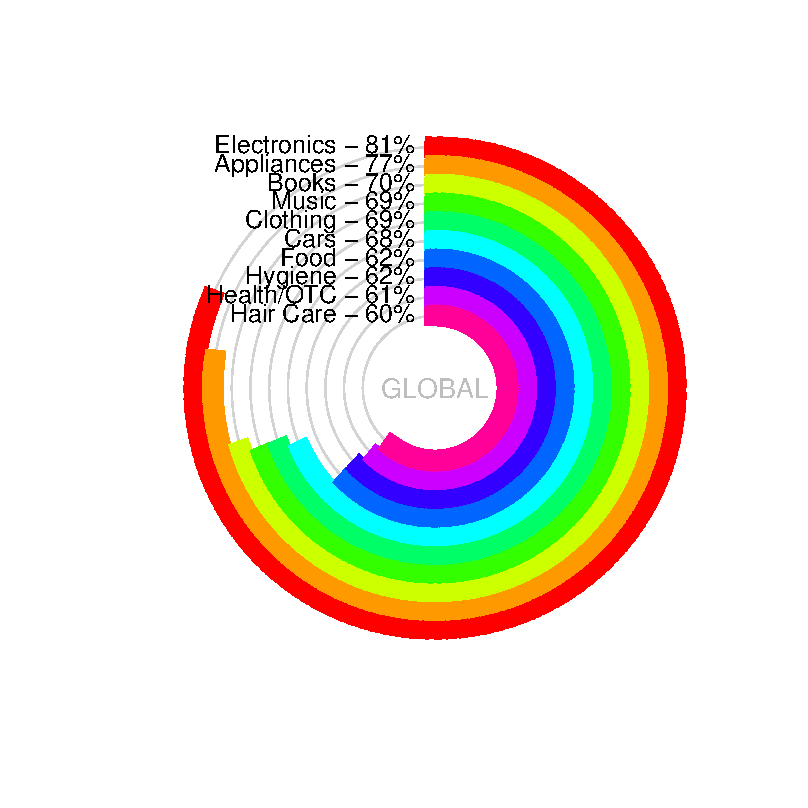
\includegraphics[width=\maxwidth]{figure/plot_plotrix_cb-1} 

}



\end{knitrout}
\begin{center}
\textbf{. . .}
\end{center}
\subsubsection{Paquete circlize}
El paquete circlize usa la filosof\'ia de descomponer el c\'irculo en figuras geom\'etricas m\'as 
simples, como l\'ineas y puntos, implementando grafos circulares a partir de gr\'aficos m\'as 
simples; ``implementa funciones gr\'aficas de bajo nivel para agregar gr\'aficos en las regiones de 
trazado circular".\cite{docu_circlize}
~\\Dichas funciones simples son: puntos, l\'ineas, rect\'angulos, texto, etc. Y, para organizar las 
regiones de trazado circulan, existen las siguientes funciones: inicializar, actualizar, trazado, 
limpiar, etc.~\\

En este apartado, se utilizar\'a las funciones de par (par\'ametros del grafo), inicializar (asigna los sectores al c\'irculo),  trazado( crear las regiones de trazado), rect\'angulos (crea las barras), texto y los ejes.~\\
Se vuelven a preparar los datos para este plot debido a como expone.(De interior a exterior)
\begin{knitrout}
\definecolor{shadecolor}{rgb}{0.969, 0.969, 0.969}\color{fgcolor}\begin{kframe}
\begin{alltt}
\hlstd{color} \hlkwb{=} \hlkwd{rainbow}\hlstd{(}\hlkwd{length}\hlstd{(Percent))}
\hlstd{Category} \hlkwb{<-} \hlkwd{rev}\hlstd{(Category)}
\hlstd{Percent} \hlkwb{<-} \hlkwd{rev}\hlstd{(Percent)}
\hlstd{color} \hlkwb{<-} \hlkwd{rev}\hlstd{(color)}
\hlkwd{library}\hlstd{(circlize)}
\end{alltt}
\end{kframe}
\end{knitrout}
\clearpage


Se inicializa el c\'irculo para que el diagrama empiece a los 90 grados. Esta parte es opcional, pues solo tiene argumentos est\'eticos y no necesarios para crear un gr\'afico con este paquete.
\begin{knitrout}
\definecolor{shadecolor}{rgb}{0.969, 0.969, 0.969}\color{fgcolor}\begin{kframe}
\begin{alltt}
\hlkwd{circos.par}\hlstd{(}\hlstr{"start.degree"} \hlstd{=} \hlnum{90}\hlstd{,} \hlkwc{cell.padding} \hlstd{=} \hlkwd{c}\hlstd{(}\hlnum{0}\hlstd{,} \hlnum{0}\hlstd{,} \hlnum{0}\hlstd{,} \hlnum{0}\hlstd{))}
\end{alltt}
\end{kframe}
\end{knitrout}
Se inicializa la plantilla del diagrama no dividiendo el anillo donde se crea el gr\'afico y fijando los l\'imites del eje X, igualando los 360 grados de la circunferencia al 100\% de los valores de las barras.
\begin{knitrout}
\definecolor{shadecolor}{rgb}{0.969, 0.969, 0.969}\color{fgcolor}\begin{kframe}
\begin{alltt}
\hlkwd{circos.initialize}\hlstd{(}\hlstr{"a"}\hlstd{,} \hlkwc{xlim} \hlstd{=} \hlkwd{c}\hlstd{(}\hlnum{0}\hlstd{,} \hlnum{100}\hlstd{))}
\end{alltt}
\end{kframe}
\end{knitrout}
La funci\'on para crear el anillo donde se va a realizar el diagrama de Barras Radiales, con los par\'ametros del l\'imite del eje Y, la altura del anillo en porcentaje (para dejar espacio en medio del diagrama), la eliminaci\'on de los bordes y el establecimiento  del inicio de la funci\'on que establece qu\'e hay dentro del anillo.
\begin{knitrout}
\definecolor{shadecolor}{rgb}{0.969, 0.969, 0.969}\color{fgcolor}\begin{kframe}
\begin{alltt}
\hlkwd{circos.track}(ylim = \hlkwd{c}(0.5, \hlkwd{length}(Percent)+0.5), track.height = 0.8, 
             bg.border = NA, panel.fun = \hlkwd{function}(x, y) \{
               xlim = CELL_META$xlim
\end{alltt}
\end{kframe}
\end{knitrout}
Se crean las barras con \texttt{circos.rect} recreando los rect\'angulos con el uso de las variables xInicial, yInicial, xFinal y yFinal, junto a la leyenda de cada una, gracias a la funci\'on \texttt{circos.text}.
\begin{knitrout}
\definecolor{shadecolor}{rgb}{0.969, 0.969, 0.969}\color{fgcolor}\begin{kframe}
\begin{alltt}
                \hlkwd{circos.rect}\hlstd{(}\hlkwd{rep}\hlstd{(}\hlnum{0}\hlstd{,} \hlnum{10}\hlstd{),} \hlnum{1}\hlopt{:}\hlnum{10} \hlopt{-} \hlnum{0.45}\hlstd{, Percent,} \hlnum{1}\hlopt{:}\hlnum{10} \hlopt{+} \hlnum{0.45}\hlstd{,}
                            \hlkwc{col} \hlstd{= color,} \hlkwc{border} \hlstd{=} \hlstr{"white"}\hlstd{)}
               \hlkwd{circos.text}\hlstd{(}\hlkwd{rep}\hlstd{(xlim[}\hlnum{1}\hlstd{],} \hlnum{10}\hlstd{),} \hlnum{1}\hlopt{:}\hlnum{10}\hlstd{,}
                           \hlkwd{paste}\hlstd{(Category,} \hlstr{" - "}\hlstd{, Percent,} \hlstr{"%"}\hlstd{),}
                           \hlkwc{facing} \hlstd{=} \hlstr{"downward"}\hlstd{,} \hlkwc{adj} \hlstd{=} \hlkwd{c}\hlstd{(}\hlnum{1.05}\hlstd{,} \hlnum{0.5}\hlstd{),} \hlkwc{cex} \hlstd{=} \hlnum{0.8}\hlstd{)}
\end{alltt}
\end{kframe}
\end{knitrout}
Para una mejor comprensi\'on se pone la leyenda del eje X por el anillo exterior, colocando dicha leyenda seg\'un el par\'ametro \texttt{break} que situa cortes cada 5 unidades.
\begin{knitrout}
\definecolor{shadecolor}{rgb}{0.969, 0.969, 0.969}\color{fgcolor}\begin{kframe}
\begin{alltt}
               breaks = \hlkwd{seq}(0, 85, by = 5)
               \hlkwd{circos.axis}(h = \hlstr{"top"}, major.at = breaks, labels = \hlkwd{paste0}(breaks, \hlstr{"%"}), 
                           labels.cex = 0.6)\})
\end{alltt}
\end{kframe}
\end{knitrout}
Y, por \'ultimo, para no crear conflictos a la hora de crear nuevos gr\'aficos con este paquete, se limpian las variables contenidas en \texttt{circos} .
\begin{knitrout}
\definecolor{shadecolor}{rgb}{0.969, 0.969, 0.969}\color{fgcolor}\begin{kframe}
\begin{alltt}
\hlkwd{circos.clear}\hlstd{()}
\end{alltt}
\end{kframe}
\end{knitrout}
\clearpage
Resultando al final en:
\begin{knitrout}
\definecolor{shadecolor}{rgb}{0.969, 0.969, 0.969}\color{fgcolor}

{\centering 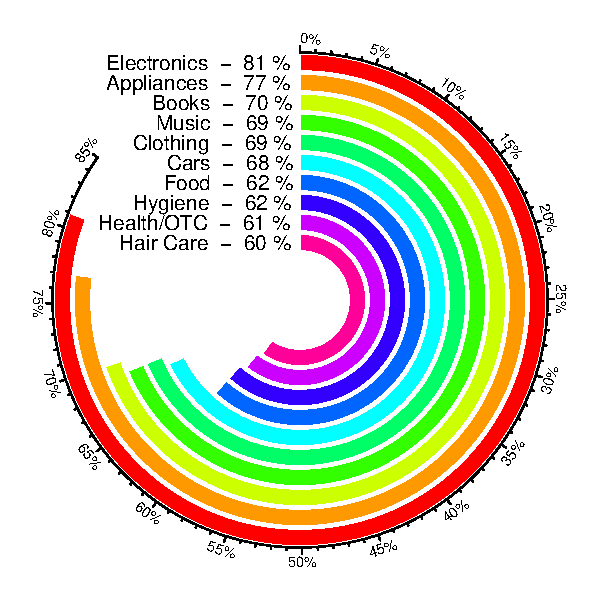
\includegraphics[width=\maxwidth]{figure/plot_circlize_cb-1} 

}



\end{knitrout}
\begin{center}
\textbf{. . .}
\end{center}
\subsubsection{Comparaciones}
Se usan tres paquetes, dos de ellos seguiran apareciendo por todo el trabajo gracias a sus versatilidad.~\\
El paquete \texttt{ggplot2}, se vuelve a usar de la misma forma que en el diagrama de anillos, reproduciendo un diagrama de barras y cambiando su sistema de coordenadas. Este paquete, en lo que a este diagrama se refiere, ofrece una gran personalizaci\'on y un correcto/facil uso de las funciones para crearlo. En uno de los ejemplos, este paquete puede juntarse con el paquete \texttt{ggiraph}, para proporcionar la variable de interactividad a este gr\'afico, ampliando su versatilidad para crear diagramas de barras radiales con gran cantidad de barras.~\\
Para el segundo paquete se ha encontrado \texttt{plotrix}; este paquete crea un gr\'afico similar a los otros dos paquetes, pero hay que ir creando los c\'irculos plantilla para despu\'es realizar los arcos que act\'uan como las barras del diagrama. Tambi\'en con este paquete la personalizaci\'on del diagrama es muy amplia.~\\
El otro paquete que se ha usado en el anterior diagrama, \texttt{circlize}, usa un m\'etodo ya explicado, que consiste en crear rect\'angulos siguiendo una plantilla circular y, al igual que en el anterior diagrama, se pueden personalizar muchos aspectos del gr\'afico.~\\
En conclusi\'on, la mejor opci\'on para crear estos diagramas de barras radiales es el paquete ggplot2, debido a la facilidad que tiene de crear los diagramas de barras tradicionales y cambiar su sistema de coordenadas.Esto lo diferencia de los otros dos. Todos los paquetes son igual de personalizables, solo que en ggplot2 es m\'as facil de realizar.
%%%%%%%%%%%%%%%%%%%%%%%%%%%%%%%%%%%%%%%%%%%%%%%%%%%%%%%%%%%%%%%%%%
\clearpage
%%%%%%%%%%%%%%%%%%%%%%%%%%%%%%%%%%%%%%%%%%%%%%%%%%%%%%%
\subsection{Diagrama Espiral}\label{ssec:espiral}
Este diagrama se puede usar para representar datos a lo largo del tiempo, por lo que la preparaci\'on de dichos datos, es lo m\'as importante en \'este. 
Para obtener este grafo, habr\'a que tener unos datos adecuados, que suelen implicar tres variables; una para ver los grados del c\'irculo, otro para su altura dentro del c\'irculo y por \'ultimo, a veces puede haber otra variable para generar el tama\~no de la figura geom\'etrica que se decida (barra, c\'irculo, etc.).
\subsubsection{Paquete ggplot2}
Se vuelve a ver este paquete\cite{docu_ggplot2}
debido a su versatilidad, pero ahora se depende mas de los datos que del paquete, este usa tres posibles generadores de barras: \texttt{rect, segment y title}~\\
Estos datos son el tiempo en movimiento de una persona durante 5 d\'ias, indicando la hora cuando se recogieron dichos datos.
\begin{knitrout}
\definecolor{shadecolor}{rgb}{0.969, 0.969, 0.969}\color{fgcolor}\begin{kframe}
\begin{alltt}
\hlkwd{library}\hlstd{(dplyr)}
\hlkwd{library}\hlstd{(readxl)}
\hlkwd{library}\hlstd{(ggplot2)}
\hlstd{dat} \hlkwb{=} \hlkwd{read_excel}\hlstd{(}\hlstr{"Data1.xlsx"}\hlstd{)}
\hlkwd{head}\hlstd{(dat,} \hlkwc{n}\hlstd{=}\hlnum{5}\hlstd{)}
\end{alltt}
\begin{verbatim}
## # A tibble: 5 x 4
##   ...1  Date1      Time  `Travel Time`   
##   <chr> <chr>      <chr> <chr>           
## 1 1     2016-09-04 13:11 34.65           
## 2 2     2016-09-04 13:12 34.35           
## 3 3     2016-09-04 13:13 33.2            
## 4 4     2016-09-04 13:14 33.0166666666667
## 5 5     2016-09-04 13:15 33.25
\end{verbatim}
\end{kframe}
\end{knitrout}

Ahora se precede a realizar la parte m\'as importante de tratar los datos para poder visualizarlos, dar a las fechas un formato m\'as manejable.
\begin{knitrout}
\definecolor{shadecolor}{rgb}{0.969, 0.969, 0.969}\color{fgcolor}\begin{kframe}
\begin{alltt}
\hlstd{dat}\hlopt{$}\hlstd{time} \hlkwb{=} \hlkwd{with}\hlstd{(dat,} \hlkwd{as.POSIXct}\hlstd{(}\hlkwd{paste}\hlstd{(Date1, Time),} \hlkwc{tz}\hlstd{=}\hlstr{"GMT"}\hlstd{))}
\end{alltt}
\end{kframe}
\end{knitrout}
Se obtienen las horas y los d\'ias.
\begin{knitrout}
\definecolor{shadecolor}{rgb}{0.969, 0.969, 0.969}\color{fgcolor}\begin{kframe}
\begin{alltt}
\hlstd{dat}\hlopt{$}\hlstd{hour} \hlkwb{=} \hlkwd{as.numeric}\hlstd{(dat}\hlopt{$}\hlstd{time)} \hlopt \hlstd{(}\hlnum{24}\hlopt{*}\hlnum{60}\hlopt{*}\hlnum{60}\hlstd{)} \hlopt{/} \hlnum{3600}
\hlstd{dat}\hlopt{$}\hlstd{day} \hlkwb{=}  \hlkwd{as.Date}\hlstd{(dat}\hlopt{$}\hlstd{time)}
\end{alltt}
\end{kframe}
\end{knitrout}
Reformar el tiempo en movimiento pasando a numeros, acortando decimales y generar tramos manejables de datos con rango de 25 min.
\begin{knitrout}
\definecolor{shadecolor}{rgb}{0.969, 0.969, 0.969}\color{fgcolor}\begin{kframe}
\begin{alltt}
\hlkwd{names}\hlstd{(dat)[}\hlkwd{grep}\hlstd{(}\hlstr{"Travel"}\hlstd{,}\hlkwd{names}\hlstd{(dat))]} \hlkwb{=} \hlstr{"TravelTime"}
\hlstd{dat}\hlopt{$}\hlstd{TravelTime} \hlkwb{=} \hlkwd{as.numeric}\hlstd{(dat}\hlopt{$}\hlstd{TravelTime)}
\hlstd{dat.smry} \hlkwb{=} \hlstd{dat} \hlopt
  \hlkwd{mutate}\hlstd{(}\hlkwc{hour.group} \hlstd{=} \hlkwd{cut}\hlstd{(hour,} \hlkwc{breaks}\hlstd{=}\hlkwd{seq}\hlstd{(}\hlnum{0}\hlstd{,}\hlnum{24}\hlstd{,}\hlnum{0.25}\hlstd{),} \hlkwc{labels}\hlstd{=}\hlkwd{seq}\hlstd{(}\hlnum{0}\hlstd{,}\hlnum{23.75}\hlstd{,}\hlnum{0.25}\hlstd{),}
                          \hlkwc{include.lowest}\hlstd{=}\hlnum{TRUE}\hlstd{),}
         \hlkwc{hour.group} \hlstd{=} \hlkwd{as.numeric}\hlstd{(}\hlkwd{as.character}\hlstd{(hour.group)))} \hlopt
  \hlkwd{group_by}\hlstd{(day, hour.group)} \hlopt
  \hlkwd{summarise}\hlstd{(}\hlkwc{meanTT} \hlstd{=} \hlkwd{mean}\hlstd{(TravelTime))} \hlopt
  \hlkwd{mutate}\hlstd{(}\hlkwc{spiralTime} \hlstd{=} \hlkwd{as.POSIXct}\hlstd{(day)} \hlopt{+} \hlstd{hour.group}\hlopt{*}\hlnum{3600}\hlstd{)}
\end{alltt}
\end{kframe}
\end{knitrout}
\clearpage
Quedando el siguiente formato de datos:
\begin{knitrout}
\definecolor{shadecolor}{rgb}{0.969, 0.969, 0.969}\color{fgcolor}\begin{kframe}
\begin{alltt}
\hlkwd{head}\hlstd{(dat,} \hlkwc{n}\hlstd{=}\hlnum{5}\hlstd{)}
\end{alltt}
\begin{verbatim}
## # A tibble: 5 x 7
##   ...1  Date1      Time  TravelTime time                 hour day       
##   <chr> <chr>      <chr>      <dbl> <dttm>              <dbl> <date>    
## 1 1     2016-09-04 13:11       34.6 2016-09-04 13:11:00  13.2 2016-09-04
## 2 2     2016-09-04 13:12       34.4 2016-09-04 13:12:00  13.2 2016-09-04
## 3 3     2016-09-04 13:13       33.2 2016-09-04 13:13:00  13.2 2016-09-04
## 4 4     2016-09-04 13:14       33.0 2016-09-04 13:14:00  13.2 2016-09-04
## 5 5     2016-09-04 13:15       33.2 2016-09-04 13:15:00  13.2 2016-09-04
\end{verbatim}
\end{kframe}
\end{knitrout}
Para el primer grafo se usar\'a el m\'etodo \texttt{rect}.

La plantilla, con los datos estableciendo las variables necesarias para crear este gr\'afico, como la x m\'inima, la x m\'axima, la y m\'inima ,delimitada por el comienzo del tiempo, la y m\'axima, por el tiempo final del diagrama, y con qu\'e variable se colorearan los rect\'angulos.
\begin{knitrout}
\definecolor{shadecolor}{rgb}{0.969, 0.969, 0.969}\color{fgcolor}\begin{kframe}
\begin{alltt}
\hlkwd{ggplot}(dat.smry, \hlkwd{aes}(xmin=\hlkwd{as.numeric}(hour.group), xmax=\hlkwd{as.numeric}(hour.group) + 0.25, 
                     ymin=spiralTime, ymax=spiralTime + meanTT*1500, fill=meanTT)) +
\end{alltt}
\end{kframe}
\end{knitrout}
Se crean las barras a cada rango de 25 minutos dado ya por los datos.
\begin{knitrout}
\definecolor{shadecolor}{rgb}{0.969, 0.969, 0.969}\color{fgcolor}\begin{kframe}
\begin{alltt}
  \hlkwd{geom_rect}(color=\hlstr{"grey40"}, size=0.2) +
\end{alltt}
\end{kframe}
\end{knitrout}
Se ajustan los ejes de las horas y la altura donde empieza cada barra.
\begin{knitrout}
\definecolor{shadecolor}{rgb}{0.969, 0.969, 0.969}\color{fgcolor}\begin{kframe}
\begin{alltt}
  \hlkwd{scale_x_continuous}(limits=\hlkwd{c}(0,24), breaks=0:23, minor_breaks=0:24,
                     labels=\hlkwd{paste0}(\hlkwd{rep}(\hlkwd{c}(12,1:11),2), \hlkwd{rep}(\hlkwd{c}(\hlstr{"AM"},\hlstr{"PM"}),each=12))) +
  \hlkwd{scale_y_datetime}(limits=\hlkwd{range}(dat.smry$spiralTime) + \hlkwd{c}(-2*24*3600,3600*19), 
                   breaks=\hlkwd{seq}(\hlkwd{min}(dat.smry$spiralTime),\hlkwd{max}(dat.smry$spiralTime),\hlstr{"1 day"}),
                   date_labels=\hlstr{"%b %e"}) +
\end{alltt}
\end{kframe}
\end{knitrout}
Se fija el color verde para los rangos de poco movimiento, amarillo medio y rojo alto.
\begin{knitrout}
\definecolor{shadecolor}{rgb}{0.969, 0.969, 0.969}\color{fgcolor}\begin{kframe}
\begin{alltt}
  \hlkwd{scale_fill_gradient2}(low=\hlstr{"green"}, mid=\hlstr{"yellow"}, high=\hlstr{"red"}, midpoint=35) +
\end{alltt}
\end{kframe}
\end{knitrout}
Y tansformar la coordenada x a sistema de coordenadas polares y se ajustan las est\'eticas del tema como el fondo, leyenda, cuadr\'icula de la escala, etc.
\begin{knitrout}
\definecolor{shadecolor}{rgb}{0.969, 0.969, 0.969}\color{fgcolor}\begin{kframe}
\begin{alltt}
  \hlkwd{coord_polar}\hlstd{()} \hlopt{+}
  \hlkwd{theme_bw}\hlstd{(}\hlkwc{base_size}\hlstd{=}\hlnum{13}\hlstd{)} \hlopt{+}
  \hlkwd{labs}\hlstd{(}\hlkwc{x}\hlstd{=}\hlstr{"Horas"}\hlstd{,}\hlkwc{y}\hlstd{=}\hlstr{"Dias"}\hlstd{,}\hlkwc{fill}\hlstd{=}\hlstr{"Media de tiempo moviendose"}\hlstd{)} \hlopt{+}
  \hlkwd{theme}\hlstd{(}\hlkwc{panel.grid.minor.x}\hlstd{=}\hlkwd{element_line}\hlstd{(}\hlkwc{colour}\hlstd{=}\hlstr{"grey60"}\hlstd{,} \hlkwc{size}\hlstd{=}\hlnum{0.3}\hlstd{))}
\end{alltt}
\end{kframe}
\end{knitrout}
\clearpage
Resultando en:
\begin{knitrout}
\definecolor{shadecolor}{rgb}{0.969, 0.969, 0.969}\color{fgcolor}

{\centering 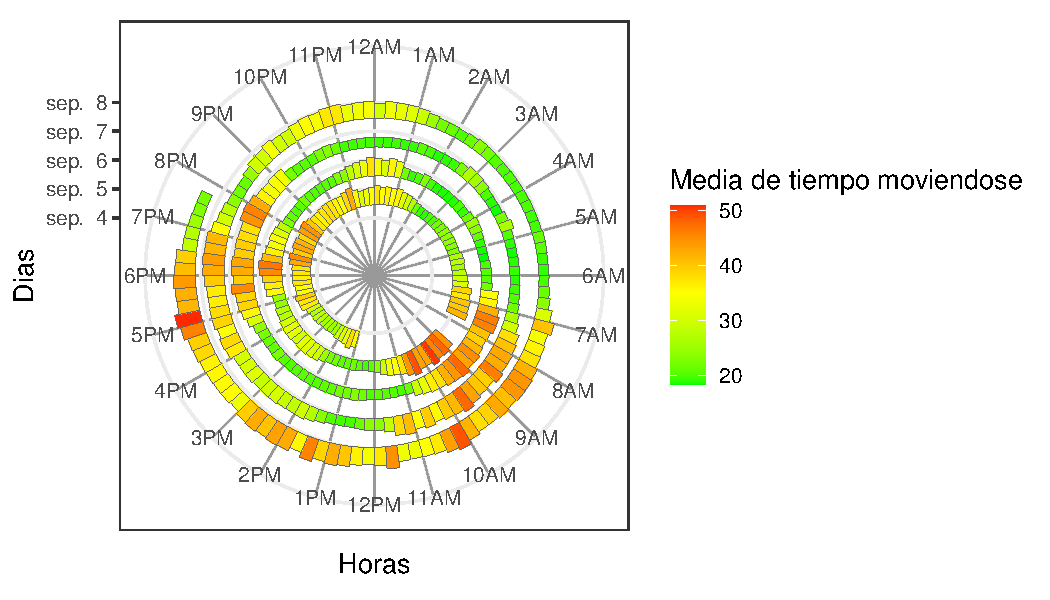
\includegraphics[width=\maxwidth]{figure/plot_rect-1} 

}



\end{knitrout}
\begin{center}
\textbf{. . .}
\end{center}
~\\
Para el segundo grafo se usar\'a el m\'etodo \texttt{segment}.

Primero se usa la misma plantilla que el ejemplo anterior.
\begin{knitrout}
\definecolor{shadecolor}{rgb}{0.969, 0.969, 0.969}\color{fgcolor}\begin{kframe}
\begin{alltt}
\hlkwd{ggplot}(dat.smry, \hlkwd{aes}(x=\hlkwd{as.numeric}(hour.group), xend=\hlkwd{as.numeric}(hour.group) + 0.25, 
                     y=spiralTime, yend=spiralTime, colour=meanTT)) +
\end{alltt}
\end{kframe}
\end{knitrout}
Luego, en vez de usar las barras se van a usar segmentos, los cuales, dejan una spiral con el mismo tama\~no, con la \'unica diferencia de los colores.
\begin{knitrout}
\definecolor{shadecolor}{rgb}{0.969, 0.969, 0.969}\color{fgcolor}\begin{kframe}
\begin{alltt}
  \hlkwd{geom_segment}(size=6) +
\end{alltt}
\end{kframe}
\end{knitrout}
Y despu\'es de usar los mismos m\'etodos que antes se obtiene el siguiente gr\'afico.
\begin{knitrout}
\definecolor{shadecolor}{rgb}{0.969, 0.969, 0.969}\color{fgcolor}\begin{kframe}
\begin{alltt}
  \hlkwd{scale_x_continuous}\hlstd{(}\hlkwc{limits}\hlstd{=}\hlkwd{c}\hlstd{(}\hlnum{0}\hlstd{,}\hlnum{24}\hlstd{),} \hlkwc{breaks}\hlstd{=}\hlnum{0}\hlopt{:}\hlnum{23}\hlstd{,} \hlkwc{minor_breaks}\hlstd{=}\hlnum{0}\hlopt{:}\hlnum{24}\hlstd{,}
                     \hlkwc{labels}\hlstd{=}\hlkwd{paste0}\hlstd{(}\hlkwd{rep}\hlstd{(}\hlkwd{c}\hlstd{(}\hlnum{12}\hlstd{,}\hlnum{1}\hlopt{:}\hlnum{11}\hlstd{),}\hlnum{2}\hlstd{),} \hlkwd{rep}\hlstd{(}\hlkwd{c}\hlstd{(}\hlstr{"AM"}\hlstd{,}\hlstr{"PM"}\hlstd{),}\hlkwc{each}\hlstd{=}\hlnum{12}\hlstd{)))} \hlopt{+}
  \hlkwd{scale_y_datetime}\hlstd{(}\hlkwc{limits}\hlstd{=}\hlkwd{range}\hlstd{(dat.smry}\hlopt{$}\hlstd{spiralTime)} \hlopt{+} \hlkwd{c}\hlstd{(}\hlopt{-}\hlnum{3}\hlopt{*}\hlnum{24}\hlopt{*}\hlnum{3600}\hlstd{,}\hlnum{0}\hlstd{),}
                   \hlkwc{breaks}\hlstd{=}\hlkwd{seq}\hlstd{(}\hlkwd{min}\hlstd{(dat.smry}\hlopt{$}\hlstd{spiralTime),} \hlkwd{max}\hlstd{(dat.smry}\hlopt{$}\hlstd{spiralTime),}\hlstr{"1 day"}\hlstd{),}
                   \hlkwc{date_labels}\hlstd{=}\hlstr{"%b %e"}\hlstd{)} \hlopt{+}
  \hlkwd{scale_colour_gradient2}\hlstd{(}\hlkwc{low}\hlstd{=}\hlstr{"green"}\hlstd{,} \hlkwc{mid}\hlstd{=}\hlstr{"yellow"}\hlstd{,} \hlkwc{high}\hlstd{=}\hlstr{"red"}\hlstd{,} \hlkwc{midpoint}\hlstd{=}\hlnum{35}\hlstd{)} \hlopt{+}
  \hlkwd{coord_polar}\hlstd{()} \hlopt{+}
  \hlkwd{theme_bw}\hlstd{(}\hlkwc{base_size}\hlstd{=}\hlnum{10}\hlstd{)} \hlopt{+}
  \hlkwd{labs}\hlstd{(}\hlkwc{x}\hlstd{=}\hlstr{"Horas"}\hlstd{,}\hlkwc{y}\hlstd{=}\hlstr{"Dias"}\hlstd{,}\hlkwc{color}\hlstd{=}\hlstr{"Media de tiempo moviendose"}\hlstd{)} \hlopt{+}
  \hlkwd{theme}\hlstd{(}\hlkwc{panel.grid.minor.x}\hlstd{=}\hlkwd{element_line}\hlstd{(}\hlkwc{colour}\hlstd{=}\hlstr{"grey60"}\hlstd{,} \hlkwc{size}\hlstd{=}\hlnum{0.3}\hlstd{))}
\end{alltt}
\end{kframe}
\end{knitrout}
\begin{knitrout}
\definecolor{shadecolor}{rgb}{0.969, 0.969, 0.969}\color{fgcolor}

{\centering 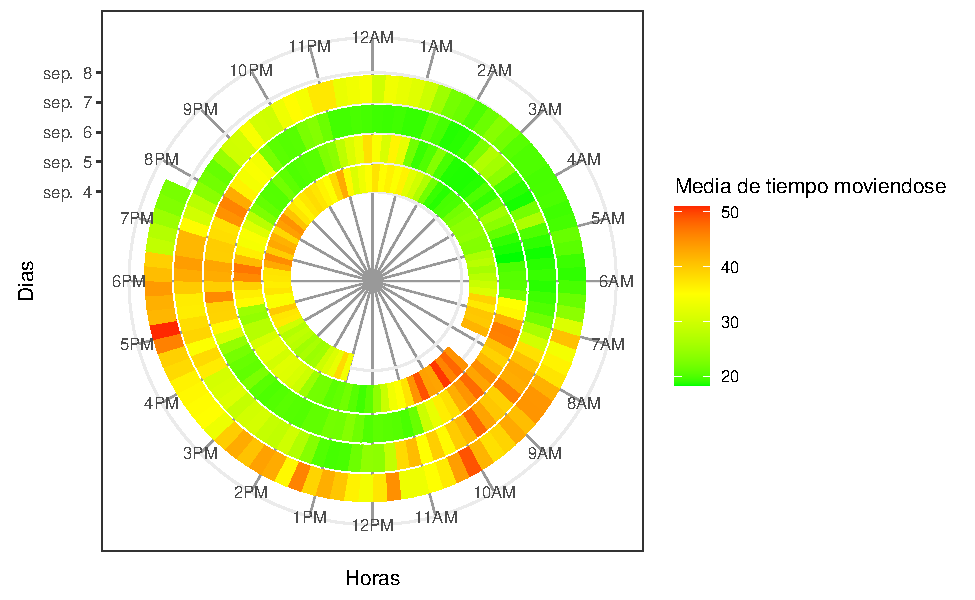
\includegraphics[width=\maxwidth]{figure/polt_segment-1} 

}



\end{knitrout}
\begin{center}
\textbf{. . .}
\end{center}
~\\
Y para el \'ultimo grafo se usar\'a el m\'etodo \texttt{title}.

Con este m\'etodo se puede variar su tama\~no para dar una forma similar al primer ejemplo.
\begin{knitrout}
\definecolor{shadecolor}{rgb}{0.969, 0.969, 0.969}\color{fgcolor}\begin{kframe}
\begin{alltt}
\hlkwd{ggplot}\hlstd{(dat.smry,} \hlkwd{aes}\hlstd{(}\hlkwc{x}\hlstd{=}\hlkwd{as.numeric}\hlstd{(hour.group)} \hlopt{+} \hlnum{0.25}\hlopt{/}\hlnum{2}\hlstd{,} \hlkwc{xend}\hlstd{=}\hlkwd{as.numeric}\hlstd{(hour.group)} \hlopt{+} \hlnum{0.25}\hlopt{/}\hlnum{2}\hlstd{,}
                     \hlkwc{y}\hlstd{=spiralTime,} \hlkwc{yend}\hlstd{=spiralTime,} \hlkwc{fill}\hlstd{=meanTT))} \hlopt{+}
  \hlkwd{geom_tile}\hlstd{(}\hlkwd{aes}\hlstd{(}\hlkwc{height}\hlstd{=meanTT}\hlopt{*}\hlnum{1800}\hlopt{*}\hlnum{0.9}\hlstd{))} \hlopt{+}
  \hlkwd{scale_x_continuous}\hlstd{(}\hlkwc{limits}\hlstd{=}\hlkwd{c}\hlstd{(}\hlnum{0}\hlstd{,}\hlnum{24}\hlstd{),} \hlkwc{breaks}\hlstd{=}\hlnum{0}\hlopt{:}\hlnum{23}\hlstd{,} \hlkwc{minor_breaks}\hlstd{=}\hlnum{0}\hlopt{:}\hlnum{24}\hlstd{,}
                     \hlkwc{labels}\hlstd{=}\hlkwd{paste0}\hlstd{(}\hlkwd{rep}\hlstd{(}\hlkwd{c}\hlstd{(}\hlnum{12}\hlstd{,}\hlnum{1}\hlopt{:}\hlnum{11}\hlstd{),}\hlnum{2}\hlstd{),} \hlkwd{rep}\hlstd{(}\hlkwd{c}\hlstd{(}\hlstr{"AM"}\hlstd{,}\hlstr{"PM"}\hlstd{),}\hlkwc{each}\hlstd{=}\hlnum{12}\hlstd{)))} \hlopt{+}
  \hlkwd{scale_y_datetime}\hlstd{(}\hlkwc{limits}\hlstd{=}\hlkwd{range}\hlstd{(dat.smry}\hlopt{$}\hlstd{spiralTime)} \hlopt{+} \hlkwd{c}\hlstd{(}\hlopt{-}\hlnum{3}\hlopt{*}\hlnum{24}\hlopt{*}\hlnum{3600}\hlstd{,}\hlnum{3600}\hlopt{*}\hlnum{9}\hlstd{),}
                   \hlkwc{breaks}\hlstd{=}\hlkwd{seq}\hlstd{(}\hlkwd{min}\hlstd{(dat.smry}\hlopt{$}\hlstd{spiralTime),}\hlkwd{max}\hlstd{(dat.smry}\hlopt{$}\hlstd{spiralTime),}\hlstr{"1 day"}\hlstd{),}
                   \hlkwc{date_labels}\hlstd{=}\hlstr{"%b %e"}\hlstd{)} \hlopt{+}
  \hlkwd{scale_fill_gradient2}\hlstd{(}\hlkwc{low}\hlstd{=}\hlstr{"green"}\hlstd{,} \hlkwc{mid}\hlstd{=}\hlstr{"yellow"}\hlstd{,} \hlkwc{high}\hlstd{=}\hlstr{"red"}\hlstd{,} \hlkwc{midpoint}\hlstd{=}\hlnum{35}\hlstd{)} \hlopt{+}
  \hlkwd{coord_polar}\hlstd{()} \hlopt{+}
  \hlkwd{theme_bw}\hlstd{(}\hlkwc{base_size}\hlstd{=}\hlnum{12}\hlstd{)} \hlopt{+}
  \hlkwd{labs}\hlstd{(}\hlkwc{x}\hlstd{=}\hlstr{"Horas"}\hlstd{,}\hlkwc{y}\hlstd{=}\hlstr{"Dias"}\hlstd{,}\hlkwc{fill}\hlstd{=}\hlstr{"Media de tiempo moviendose"}\hlstd{)} \hlopt{+}
  \hlkwd{theme}\hlstd{(}\hlkwc{panel.grid.minor.x}\hlstd{=}\hlkwd{element_line}\hlstd{(}\hlkwc{colour}\hlstd{=}\hlstr{"grey60"}\hlstd{,} \hlkwc{size}\hlstd{=}\hlnum{0.3}\hlstd{))}
\end{alltt}
\end{kframe}
\end{knitrout}
\clearpage
Dando el resultado de:~\\
\begin{knitrout}
\definecolor{shadecolor}{rgb}{0.969, 0.969, 0.969}\color{fgcolor}

{\centering 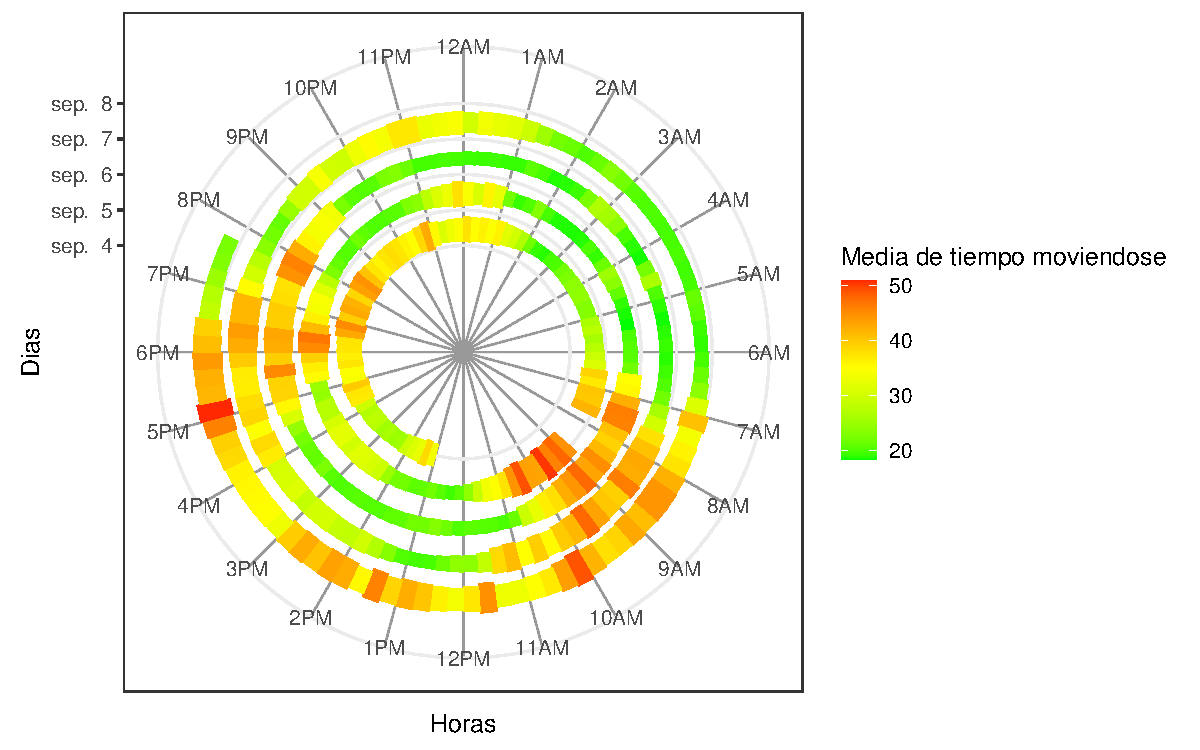
\includegraphics[width=\maxwidth]{figure/plot_title-1} 

}



\end{knitrout}
%%%%%%%%%%%%%%%%%%%%%%%%%%%%%%%%%%%%%%%%%%%%%%%%%%%%%%%%%%%%%%%%%%hecho
\clearpage
%%%%%%%%%%%%%%%%%%%%%%%%%%%%%%%%%%%%%%%%%%%%%%%%%%%%%%%
\subsection{Diagrama de Columnas Radiales}\label{ssec:columnasRadiales}
Este diagrama es una variante de los diagramas m\'as usados (diagrama de barras) y, como se vi\'o en el apartado \autoref{ssec:barrasRadiales}
, esta es otra variante que en vez de posicionar el valor de las barras en el eje X lo situ\'a en el eje Y quedando el eje X para los nombres de las barras.
Para realizar este tipo de diagramas, la gran mayoria de paquetes lo afrontan creando un diagrama de barras con sistema de coordenadas cartesianas y transforman el sistema del eje X a polares, pero otros paquetes simplemente crear el diagrama cambiando la direcci\'on de las barras.
\subsubsection{Paquete ggplot2}
Con este paquete \cite{docu_ggplot2}
se procede a copiar la manera de crear el diagrama de Barras Radiales \autoref{ssec:barrasRadiales}
 pero, en esta ocasi\'on, la coordenada a transformar esta vez se la X.~\\
Primero se va a crear los datos de ejemplo para representar en este gr\'afico, estableciendo las entidades (barras), sus valores y el grupo al que pertenecen las barras, junto con la llamada de la libreria.
\begin{knitrout}
\definecolor{shadecolor}{rgb}{0.969, 0.969, 0.969}\color{fgcolor}\begin{kframe}
\begin{alltt}
\hlstd{data} \hlkwb{<-} \hlkwd{data.frame}\hlstd{(}
  \hlkwc{id}\hlstd{=}\hlkwd{seq}\hlstd{(}\hlnum{1}\hlstd{,}\hlnum{20}\hlstd{),}
  \hlkwc{individual}\hlstd{=}\hlkwd{paste}\hlstd{(} \hlstr{"Colum. "}\hlstd{,} \hlkwd{seq}\hlstd{(}\hlnum{1}\hlstd{,}\hlnum{20}\hlstd{),} \hlkwc{sep}\hlstd{=}\hlstr{""}\hlstd{),}
  \hlkwc{group}\hlstd{=}\hlkwd{c}\hlstd{(} \hlkwd{rep}\hlstd{(}\hlstr{'A'}\hlstd{,} \hlnum{5}\hlstd{),} \hlkwd{rep}\hlstd{(}\hlstr{'B'}\hlstd{,} \hlnum{8}\hlstd{),} \hlkwd{rep}\hlstd{(}\hlstr{'C'}\hlstd{,} \hlnum{5}\hlstd{),} \hlkwd{rep}\hlstd{(}\hlstr{'D'}\hlstd{,} \hlnum{2}\hlstd{)) ,}
  \hlkwc{value}\hlstd{=}\hlkwd{sample}\hlstd{(} \hlkwd{seq}\hlstd{(}\hlnum{10}\hlstd{,}\hlnum{50}\hlstd{),} \hlnum{20}\hlstd{,} \hlkwc{replace}\hlstd{=T)}
\hlstd{)}
\hlkwd{library}\hlstd{(ggplot2)}
\end{alltt}
\end{kframe}
\end{knitrout}

Para implementar este gr\'afico se escogen los datos, asignando los ejes correspondientes y la figura geom\'etricas de la barra.
\begin{knitrout}
\definecolor{shadecolor}{rgb}{0.969, 0.969, 0.969}\color{fgcolor}\begin{kframe}
\begin{alltt}
\hlkwd{ggplot}(data, \hlkwd{aes}(x=\hlkwd{as.factor}(id), y=value)) +
  \hlkwd{geom_bar}(stat=\hlstr{"identity"}, fill=\hlkwd{alpha}(\hlstr{"blue"},0.2)) +
\end{alltt}
\end{kframe}
\end{knitrout}
Esta vez se puede controlar el espacio del centro mediante la variable \texttt{ylim}, en lugar de tener que rellenar los datos con valores vac\'ios para luego no representarlos.
\begin{knitrout}
\definecolor{shadecolor}{rgb}{0.969, 0.969, 0.969}\color{fgcolor}\begin{kframe}
\begin{alltt}
  \hlkwd{ylim}(-10,60) +
\end{alltt}
\end{kframe}
\end{knitrout}
Se transforma el eje x de lineal a radial y se hace coincidir el principio del gr\'afico con el principio del c\'irculo (0 grados).
\begin{knitrout}
\definecolor{shadecolor}{rgb}{0.969, 0.969, 0.969}\color{fgcolor}\begin{kframe}
\begin{alltt}
  \hlkwd{coord_polar}(start = 0) +
\end{alltt}
\end{kframe}
\end{knitrout}
Y, por \'ultimo, se ajusta la est\'etica deseada ajustando el fondo y elementos como la leyenda y el texto de los ejes.
\begin{knitrout}
\definecolor{shadecolor}{rgb}{0.969, 0.969, 0.969}\color{fgcolor}\begin{kframe}
\begin{alltt}
  \hlkwd{theme_minimal}\hlstd{()} \hlopt{+}
  \hlkwd{theme}\hlstd{(}
    \hlkwc{axis.text} \hlstd{=} \hlkwd{element_blank}\hlstd{(),}
    \hlkwc{axis.title} \hlstd{=} \hlkwd{element_blank}\hlstd{(),}
    \hlkwc{panel.grid} \hlstd{=} \hlkwd{element_blank}\hlstd{(),}
    \hlkwc{plot.margin} \hlstd{=} \hlkwd{unit}\hlstd{(}\hlkwd{rep}\hlstd{(}\hlopt{-}\hlnum{2}\hlstd{,}\hlnum{4}\hlstd{),} \hlstr{"cm"}\hlstd{)}
  \hlstd{)}
\end{alltt}
\end{kframe}
\end{knitrout}
\clearpage
Quedando el gr\'afico de la siguiente forma.
\begin{knitrout}
\definecolor{shadecolor}{rgb}{0.969, 0.969, 0.969}\color{fgcolor}

{\centering 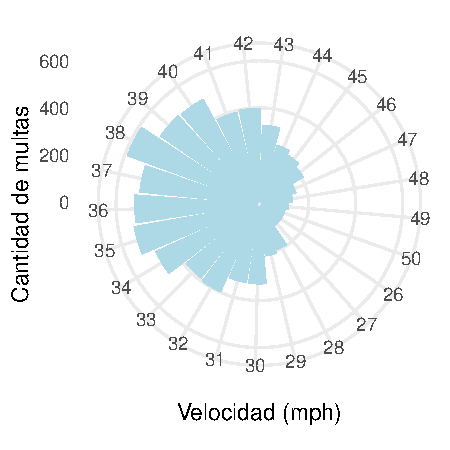
\includegraphics[width=\maxwidth]{figure/plot_ggplot_cr-1} 

}



\end{knitrout}
\begin{center}
\textbf{. . .}
\end{center}
~\\
Como se ha observado con anterioridad, este paquete deja mucho espacio para la personalizaci\'on de estos gr\'aficos, por lo que se va a implementar el mismo gr\'afico que antes con grupos con espacios diferenciados y etiquetas.~\\
 Para crear los espacios entre los grupos, se va a a\~nadir al igual que en el diagrama de barras radiales, barras con datos vac\'ios para que dejen el espacio al no ser representados.
\begin{knitrout}
\definecolor{shadecolor}{rgb}{0.969, 0.969, 0.969}\color{fgcolor}\begin{kframe}
\begin{alltt}
\hlkwd{library}\hlstd{(tidyverse)}
\hlstd{empty_bar} \hlkwb{<-} \hlnum{4}
\hlstd{to_add} \hlkwb{<-} \hlkwd{data.frame}\hlstd{(} \hlkwd{matrix}\hlstd{(}\hlnum{NA}\hlstd{, empty_bar}\hlopt{*}\hlkwd{nlevels}\hlstd{(data}\hlopt{$}\hlstd{group),} \hlkwd{ncol}\hlstd{(data)) )}
\hlkwd{colnames}\hlstd{(to_add)} \hlkwb{<-} \hlkwd{colnames}\hlstd{(data)}
\hlstd{to_add}\hlopt{$}\hlstd{group} \hlkwb{<-} \hlkwd{rep}\hlstd{(}\hlkwd{levels}\hlstd{(data}\hlopt{$}\hlstd{group),} \hlkwc{each}\hlstd{=empty_bar)}
\hlstd{datatrans} \hlkwb{<-} \hlkwd{rbind}\hlstd{(data, to_add)}
\hlstd{datatrans} \hlkwb{<-} \hlstd{datatrans} \hlopt \hlkwd{arrange}\hlstd{(group)}
\hlstd{datatrans}\hlopt{$}\hlstd{id} \hlkwb{<-} \hlkwd{seq}\hlstd{(}\hlnum{1}\hlstd{,} \hlkwd{nrow}\hlstd{(datatrans))}
\end{alltt}
\end{kframe}
\end{knitrout}
Para la parte de las etiquetas habr\'a que poner el datos que se quiera visualizar en todas las columnas y ajustar su altura y \'angulo
\begin{knitrout}
\definecolor{shadecolor}{rgb}{0.969, 0.969, 0.969}\color{fgcolor}\begin{kframe}
\begin{alltt}
\hlstd{label_data} \hlkwb{<-} \hlstd{datatrans}
\hlstd{number_of_bar} \hlkwb{<-} \hlkwd{nrow}\hlstd{(label_data)}
\hlstd{angle} \hlkwb{<-} \hlnum{90} \hlopt{-} \hlnum{360} \hlopt{*} \hlstd{(label_data}\hlopt{$}\hlstd{id}\hlopt{-}\hlnum{0.5}\hlstd{)} \hlopt{/}\hlstd{number_of_bar}
\hlstd{label_data}\hlopt{$}\hlstd{hjust} \hlkwb{<-} \hlkwd{ifelse}\hlstd{( angle} \hlopt{< -}\hlnum{90}\hlstd{,} \hlnum{1}\hlstd{,} \hlnum{0}\hlstd{)}
\hlstd{label_data}\hlopt{$}\hlstd{angle} \hlkwb{<-} \hlkwd{ifelse}\hlstd{(angle} \hlopt{< -}\hlnum{90}\hlstd{, angle}\hlopt{+}\hlnum{180}\hlstd{, angle)}
\end{alltt}
\end{kframe}
\end{knitrout}
Para ahora crear el gr\'afico usamos las siguentes funciones.

Lo primero que es distinto es el hecho de que pinta las columnas dependiendo del grupo.
\begin{knitrout}
\definecolor{shadecolor}{rgb}{0.969, 0.969, 0.969}\color{fgcolor}\begin{kframe}
\begin{alltt}
\hlkwd{ggplot}(datatrans, \hlkwd{aes}(x=\hlkwd{as.factor}(id), y=value, fill=group)) +
  \hlkwd{geom_bar}(stat=\hlstr{"identity"}, alpha=0.5) +
\end{alltt}
\end{kframe}
\end{knitrout}
\clearpage
Por lo dem\'as, todo es igual hasta que se a\~nade la \'ultima funci\'on, la cual genera las etiquetas del gr\'afico ajustadas a la altura y el \'angulo.
\begin{knitrout}
\definecolor{shadecolor}{rgb}{0.969, 0.969, 0.969}\color{fgcolor}\begin{kframe}
\begin{alltt}
  \hlkwd{geom_text}\hlstd{(}\hlkwc{data}\hlstd{=label_data,} \hlkwd{aes}\hlstd{(}\hlkwc{x}\hlstd{=id,} \hlkwc{y}\hlstd{=value}\hlopt{+}\hlnum{10}\hlstd{,} \hlkwc{label}\hlstd{=individual,} \hlkwc{hjust}\hlstd{=hjust),}
      \hlkwc{color}\hlstd{=}\hlstr{"black"}\hlstd{,} \hlkwc{fontface}\hlstd{=}\hlstr{"bold"}\hlstd{,}\hlkwc{alpha}\hlstd{=}\hlnum{0.6}\hlstd{,} \hlkwc{size}\hlstd{=}\hlnum{2.5}\hlstd{,} \hlkwc{angle}\hlstd{= label_data}\hlopt{$}\hlstd{angle,}
      \hlkwc{inherit.aes} \hlstd{=} \hlnum{FALSE} \hlstd{)}
\end{alltt}
\end{kframe}
\end{knitrout}
Resultando en este \'ultimo gr\'afico
\begin{knitrout}
\definecolor{shadecolor}{rgb}{0.969, 0.969, 0.969}\color{fgcolor}

{\centering 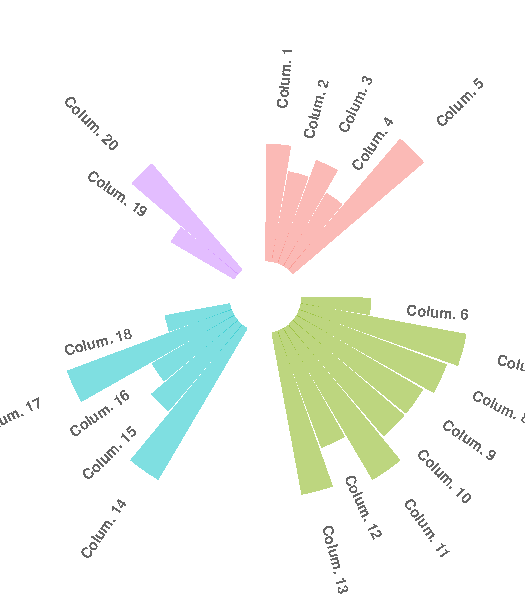
\includegraphics[width=\maxwidth]{figure/plot_ggplot_final_cr-1} 

}



\end{knitrout}
\begin{center}
\textbf{. . .}
\end{center}
~\\
Existe una forma de realizar este mismo gr\'afico con interactividad con la ayuda de ggplot2 y ggiraph. Ya se ha explicado en otros diagramas com\'o, asi que, en este solo se ense\~na el resultado.
\begin{knitrout}
\definecolor{shadecolor}{rgb}{0.969, 0.969, 0.969}\color{fgcolor}\begin{kframe}
\begin{alltt}
\hlkwd{library}\hlstd{(ggiraph)}
\hlstd{p} \hlkwb{<-} \hlkwd{ggplot}\hlstd{(data,} \hlkwd{aes}\hlstd{(}\hlkwc{x}\hlstd{=}\hlkwd{as.factor}\hlstd{(id),} \hlkwc{y}\hlstd{=value,} \hlkwc{tooltip}\hlstd{=}\hlkwd{as.factor}\hlstd{(id),}
                      \hlkwc{data_id} \hlstd{=} \hlkwd{as.factor}\hlstd{(id),} \hlkwc{fill} \hlstd{= group))} \hlopt{+}
  \hlkwd{geom_col_interactive}\hlstd{()} \hlopt{+}
  \hlkwd{ylim}\hlstd{(}\hlopt{-}\hlnum{10}\hlstd{,}\hlnum{60}\hlstd{)} \hlopt{+}
  \hlkwd{coord_polar}\hlstd{(}\hlkwc{start} \hlstd{=} \hlnum{0}\hlstd{)} \hlopt{+}
  \hlkwd{theme_minimal}\hlstd{()} \hlopt{+}
  \hlkwd{theme}\hlstd{(}
    \hlkwc{axis.text} \hlstd{=} \hlkwd{element_blank}\hlstd{(),}
    \hlkwc{axis.title} \hlstd{=} \hlkwd{element_blank}\hlstd{(),}
    \hlkwc{panel.grid} \hlstd{=} \hlkwd{element_blank}\hlstd{(),}
    \hlkwc{plot.margin} \hlstd{=} \hlkwd{unit}\hlstd{(}\hlkwd{rep}\hlstd{(}\hlopt{-}\hlnum{2}\hlstd{,}\hlnum{4}\hlstd{),} \hlstr{"cm"}\hlstd{)}
  \hlstd{)}
\hlkwd{girafe}\hlstd{(}\hlkwc{ggobj} \hlstd{= p)}
\end{alltt}
\end{kframe}
\end{knitrout}
\vbox{
    \centering
    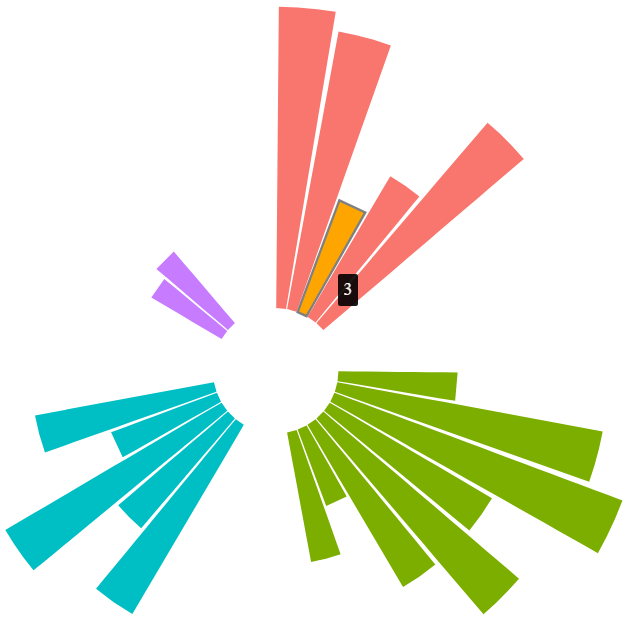
\includegraphics[width=0.5\textwidth]{imag/ggplot2_inte_cr}
}
\begin{center}
\textbf{. . .}
\end{center}
\subsubsection{Paquete plotrix}
Como se dijo, \autoref{ssec:barrasRadiales}
, este paquete ser\'ia usado para otros gr\'aficos m\'as adelante por sus plots espec\'ificos. Y gracias a las funciones \texttt{polar plot} y \texttt{radial plot} se pude contar con \'el en este apartado. 
Para ello se establecen los datos usados.~\\
Primero la longitud de las columnas con n\'umeros aleatorios.
\begin{knitrout}
\definecolor{shadecolor}{rgb}{0.969, 0.969, 0.969}\color{fgcolor}\begin{kframe}
\begin{alltt}
\hlstd{long} \hlkwb{<-} \hlkwd{c}\hlstd{(}\hlkwd{rnorm}\hlstd{(}\hlnum{36}\hlstd{)}\hlopt{*}\hlnum{2}\hlopt{+}\hlnum{5}\hlstd{)}
\end{alltt}
\end{kframe}
\end{knitrout}
Luego la posici\'on de cada columna en el c\'irculo, siempre en grados.
\begin{knitrout}
\definecolor{shadecolor}{rgb}{0.969, 0.969, 0.969}\color{fgcolor}\begin{kframe}
\begin{alltt}
\hlstd{pos} \hlkwb{<-} \hlkwd{seq}\hlstd{(}\hlnum{0}\hlstd{,}\hlnum{350}\hlstd{,}\hlkwc{by}\hlstd{=}\hlnum{10}\hlstd{)}
\end{alltt}
\end{kframe}
\end{knitrout}
Para luego usar las dos funciones, estas son capaces de usar los mismos par\'ametros.
\begin{knitrout}
\definecolor{shadecolor}{rgb}{0.969, 0.969, 0.969}\color{fgcolor}\begin{kframe}
\begin{alltt}
\hlkwd{library}\hlstd{(plotrix)}
\hlkwd{polar.plot}\hlstd{(long, pos,}\hlkwc{main}\hlstd{=}\hlstr{"Polar Plot"}\hlstd{,}\hlkwc{lwd}\hlstd{=}\hlnum{3}\hlstd{,}\hlkwc{line.col}\hlstd{=}\hlnum{2}\hlstd{,}
           \hlkwc{rad.col}\hlstd{=} \hlstr{"lightblue"}\hlstd{,} \hlkwc{grid.col}\hlstd{=} \hlstr{"lightblue"}\hlstd{,}\hlkwc{start} \hlstd{=} \hlnum{0}\hlstd{)}
\end{alltt}
\end{kframe}

{\centering 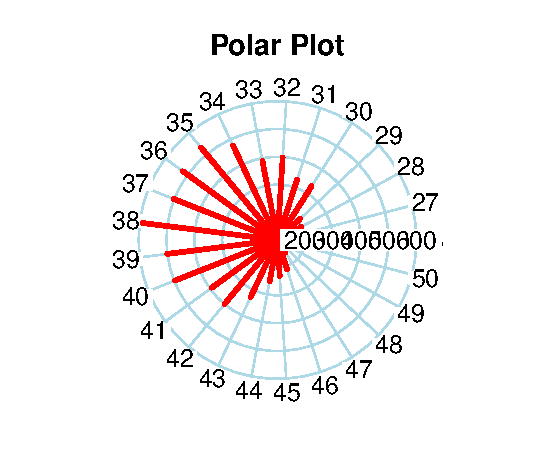
\includegraphics[width=\maxwidth]{figure/plot_plotrix_cr-1} 

}


\begin{kframe}\begin{alltt}
\hlkwd{radial.plot}\hlstd{(long, pos,}\hlkwc{main}\hlstd{=}\hlstr{"Radial Plot"}\hlstd{,}\hlkwc{lwd}\hlstd{=}\hlnum{3}\hlstd{,}\hlkwc{line.col}\hlstd{=}\hlnum{2}\hlstd{,}
           \hlkwc{rad.col}\hlstd{=} \hlstr{"lightblue"}\hlstd{,} \hlkwc{grid.col}\hlstd{=} \hlstr{"lightblue"}\hlstd{,} \hlkwc{start} \hlstd{=} \hlnum{0}\hlstd{)}
\end{alltt}
\end{kframe}

{\centering 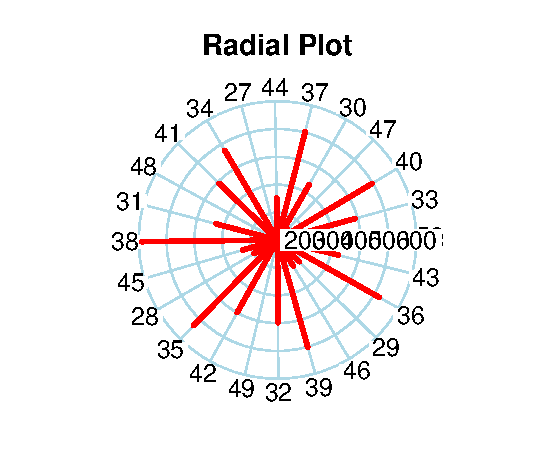
\includegraphics[width=\maxwidth]{figure/plot_plotrix_cr-2} 

}



\end{knitrout}
C\'omo se ve, los gr\'aficos no han salido iguales y es debido a que \texttt{polar plot} transforma la posici\'on de los grados a radianes mediante la funci\'on \texttt{radial plot}, pero con \texttt{radial plot} la variable \texttt{pos} se interpreta como radianes y no grados.
\clearpage
\subsubsection{Paquete cplots}
Este paquete, tal y como dice su documentaci\'on \cite{docu_cplot}
, proporciona algunos diagramas circulares provenientes de datos circulares, incluyendo diagramas de barras, de densidad, puntos apilados, etc.~\\
Para reproducir este diagrama con este paquete se debe preparar los datos.
\begin{knitrout}
\definecolor{shadecolor}{rgb}{0.969, 0.969, 0.969}\color{fgcolor}\begin{kframe}
\begin{alltt}
\hlkwd{library}\hlstd{(cplots)}
\hlkwd{library}\hlstd{(circular)}
\hlstd{x} \hlkwb{=} \hlkwd{c}\hlstd{(}\hlkwd{rvonmises}\hlstd{(}\hlnum{2000}\hlstd{,} \hlkwd{circular}\hlstd{(}\hlnum{2}\hlopt{*}\hlstd{pi}\hlopt{/}\hlnum{3}\hlstd{),} \hlnum{2}\hlstd{),}
      \hlkwd{rvonmises}\hlstd{(}\hlnum{2000}\hlstd{,} \hlkwd{circular}\hlstd{(}\hlnum{3}\hlopt{*}\hlstd{pi}\hlopt{/}\hlnum{2}\hlstd{),} \hlnum{5}\hlstd{))}
\end{alltt}
\end{kframe}
\end{knitrout}
La funci\'on \texttt{rvonmises} est\'a dentro del paquete \texttt{circular} y sirve para tener datos de forma circular donde se introduce el n\'umero de muestreos, la distribuci\'on de las muestras indicando en radianes donde se encuentra dentro del c\'irculo y la concentraci\'on de las muestras a la distribuci\'on pasada.~\\
Y para crear el gr\'afico de columnas radiales se usa \texttt{cbarplot}, el cual necesita los datos anteriores y se puede personalizar un poco como el color, la leyenda, etc.
\begin{knitrout}
\definecolor{shadecolor}{rgb}{0.969, 0.969, 0.969}\color{fgcolor}\begin{kframe}
\begin{alltt}
\hlkwd{cbarplot}\hlstd{(x,} \hlkwc{radius}\hlstd{=}\hlnum{0.5}\hlstd{,} \hlkwc{nlabels}\hlstd{=}\hlnum{3}\hlstd{,} \hlkwc{col}\hlstd{=}\hlstr{"lightblue"}\hlstd{,} \hlkwc{border}\hlstd{=}\hlstr{"skyblue4"}\hlstd{)}
\end{alltt}
\end{kframe}

{\centering 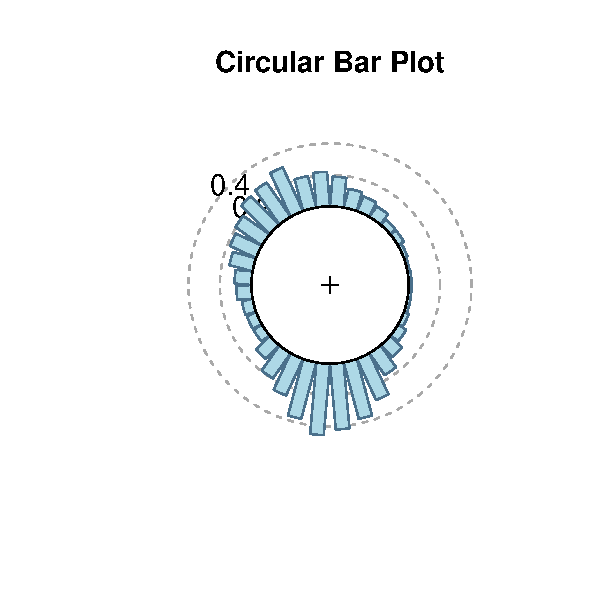
\includegraphics[width=\maxwidth]{figure/plot_cplots_cr-1} 

}



\end{knitrout}
\clearpage
Y si \texttt{nlabels} se iguala a 0 visualiza los radianes en el circulo.
\begin{knitrout}
\definecolor{shadecolor}{rgb}{0.969, 0.969, 0.969}\color{fgcolor}\begin{kframe}
\begin{alltt}
\hlkwd{cbarplot}\hlstd{(x,} \hlkwc{radius}\hlstd{=}\hlnum{0.5}\hlstd{,} \hlkwc{nlabels}\hlstd{=}\hlnum{0}\hlstd{,} \hlkwc{col}\hlstd{=}\hlstr{"lightblue"}\hlstd{)}
\end{alltt}
\end{kframe}

{\centering 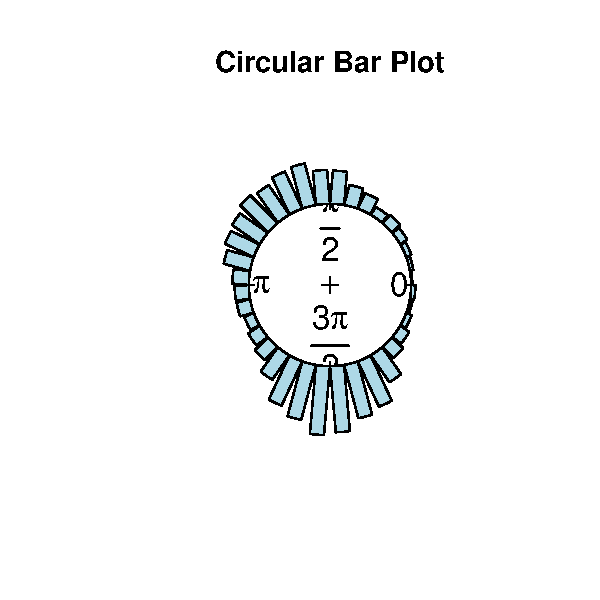
\includegraphics[width=\maxwidth]{figure/plot_cplots_cr1-1} 

}



\end{knitrout}
\begin{center}
\textbf{. . .}
\end{center}
\subsubsection{Paquete circlize}

De nuevo se utiliza este paquete\cite{docu_circlize}
de la misma forma que se utilizaba ggplot2, cambiando los ejes para representar columnas en vez de barras. Para los datos y capacidad de comparaci\'on de paquetes se eligen los mismos datos que en el primer ejemplo del paquete ggplot2.~\\
Lo primera funci\'on es opcional, ya que declara argumentos que son est\'eticos, como, en este caso, en que \'angulo comienza el diagrama, o tambi\'en, por ejemplo, se puede establecer donde est\'a en centro del diagrama.
\begin{knitrout}
\definecolor{shadecolor}{rgb}{0.969, 0.969, 0.969}\color{fgcolor}\begin{kframe}
\begin{alltt}
\hlkwd{library}\hlstd{(circlize)}
\hlkwd{circos.par}\hlstd{(}\hlstr{"start.degree"} \hlstd{=} \hlnum{90}\hlstd{)}
\end{alltt}
\end{kframe}
\end{knitrout}
Lo que si que se necesita hacer es inicializar la plantilla del gr\'afico fijando en cuantos sectores se divide cada anillo del diagrama, en este caso solo uno para crear todas las columnas en el mismo sector. Y se fijan los l\'imites del eje X desde 0 a 20.
\begin{knitrout}
\definecolor{shadecolor}{rgb}{0.969, 0.969, 0.969}\color{fgcolor}\begin{kframe}
\begin{alltt}
\hlkwd{circos.initialize}\hlstd{(}\hlstr{"a"}\hlstd{,} \hlkwc{xlim} \hlstd{=} \hlkwd{c}\hlstd{(}\hlnum{0.5}\hlstd{,} \hlkwd{length}\hlstd{(data}\hlopt{$}\hlstd{id)}\hlopt{+}\hlnum{0.5}\hlstd{))}
\end{alltt}
\end{kframe}
\end{knitrout}
\clearpage
Ahora se establece el anillo fijando el l\'imite del eje Y y la altura del anillo en porcentaje, en este caso un 80\% dejando un hueco del 20\%. Para este ejemplo se elimina el borde del anillo y la funci\'on para implementar las barras dentro del anillo.
\begin{knitrout}
\definecolor{shadecolor}{rgb}{0.969, 0.969, 0.969}\color{fgcolor}\begin{kframe}
\begin{alltt}
\hlkwd{circos.track}(ylim = \hlkwd{c}(0, 50), track.height = 0.8, 
             bg.border = NA, panel.fun = \hlkwd{function}(x, y) \{
\end{alltt}
\end{kframe}
\end{knitrout}
La funci\'on \texttt{circos.rect} realiza ret\'angulos igual que se us\'o en el diagrama de Barras Radiales, pero cambiando los ejes, poniendo esta vez en el eje X la cantidad de barras y en el eje Y los valores. Para implementarlas se pasan como argumentos xInicial, yInicial, xFinal y yFinal; con un color agradable y borde blanco para facil separaci\'on de las barras.
\begin{knitrout}
\definecolor{shadecolor}{rgb}{0.969, 0.969, 0.969}\color{fgcolor}\begin{kframe}
\begin{alltt}
               xlim = CELL_META$xlim
               \hlkwd{circos.rect}( 1:\hlkwd{length}(data$id) - 0.45,\hlkwd{rep}(0, \hlkwd{length}(data$id)), 
                 1:\hlkwd{length}(data$id) + 0.45, data$value,col = \hlstr{"skyblue"}, border = \hlstr{"white"})\})
\end{alltt}
\end{kframe}
\end{knitrout}
Y para que se pueda implementar otro ejemplo hay que limpiar las variables que est\'an en circos.
\begin{knitrout}
\definecolor{shadecolor}{rgb}{0.969, 0.969, 0.969}\color{fgcolor}\begin{kframe}
\begin{alltt}
\hlkwd{circos.clear}\hlstd{()}
\end{alltt}
\end{kframe}
\end{knitrout}
Resultando en:
\begin{knitrout}
\definecolor{shadecolor}{rgb}{0.969, 0.969, 0.969}\color{fgcolor}

{\centering 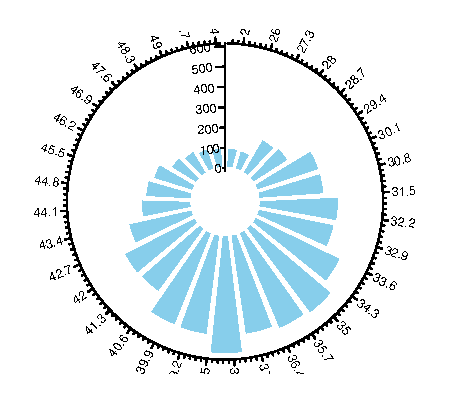
\includegraphics[width=\maxwidth]{figure/circlize_colum-1} 

}



\end{knitrout}
\begin{center}
\textbf{. . .}
\end{center}
\subsubsection{Comparaciones}
Para realizar este diagrama se han encontrado 4 paquetes; cada uno genera una aproximaci\'on diferente.
Al igual que en \nameref{ssec:barrasRadiales}, 
el paquete \texttt{ggplot2} se usa mediante la transformaci\'on del sistema de coordenadas, esto proporciona m\'as versatilidad debido a su capacidad de personalizaci\'on. En la forma de representar los datos, los tres paquetes tienen diferentes maneras de crear el diagrama; \texttt{ggplot2} ejemplifica las columnas mediante barras resultando m\'as est\'etico, \texttt{plotrix} representa las columnas con l\'ineas no dejando que cada una de las l\'ineas cambie el color ni ancho para representar importancia, y \texttt{cplots} utiliza el diagrama de histograma con formato circular, pero solo puede represenar datos con alg\'un tipo de distribuci\'on no pudiendo utilizar cualquier dato. ~\\
El paquete \texttt{circlize} es muy parecido a ggplot2 ya que los dos son complejos y completos, por su gran capacidad de personalizaci\'on, por el poder de retocar casi cualquier aspecto.~\\
En conclusi\'on, de los cuatro paquetes presentados los que resultan m\'as utiles a la hora de representar el diagrama de columnas radiales son \texttt{ggplot2} y \texttt{circlize}, por su facilidad de uso cuando ya se conocen sus funciones, y la gran capacidad de personalizaci\'on. Para diferenciar entre los dos es importante saber, que el paquete ggplot2 junto al paquete de ggiraph a\~nade la capacidad interactiva, y el hecho que sus ejemplos se pueden almacenar en una variable para poder ser usada en un futuro o modificada sin necesidad de escribrir de nuevo el c\'odigo.
%%%%%%%%%%%%%%%%%%%%%%%%%%%%%%%%%%%%%%%%%%%%%%%%%%%%%%%%%%%%%%%%%%
\clearpage
%%%%%%%%%%%%%%%%%%%%%%%%%%%%%%%%%%%%%%%%%%%%%%%%%%%%%%%
\subsection{Diagrama de Sectores}\label{ssec:sectores}
Para crear este tipo de diagramas, casi siempre se necesita de la misma estructura de datos, unas veces son simplemente unos valores represent\'andolos como un porcentaje del total de la suma de todos los valores, o pueden estar acompa\~nados de las categor\'ias correspondientes.
\subsubsection{R B\'asico}
Una de las formar m\'as sencillas para representar los diagramas de sectores es la funci\'on \texttt{pie}. Esta funci\'on necesita de los propios valores dichos antes y se pueden a\~nadir m\'as par\'ametros para su personalizaci\'on, como las etiquetas, colores y bordes.
\begin{knitrout}
\definecolor{shadecolor}{rgb}{0.969, 0.969, 0.969}\color{fgcolor}\begin{kframe}
\begin{alltt}
\hlstd{Porcentaje} \hlkwb{<-} \hlkwd{c}\hlstd{(}\hlnum{3}\hlstd{,}\hlnum{7}\hlstd{,}\hlnum{9}\hlstd{,}\hlnum{1}\hlstd{,}\hlnum{2}\hlstd{)}
\end{alltt}
\end{kframe}
\end{knitrout}
Para mejores colores y una paleta uniforme se opta por el paquete \texttt{RColorBrewer}.
\begin{knitrout}
\definecolor{shadecolor}{rgb}{0.969, 0.969, 0.969}\color{fgcolor}\begin{kframe}
\begin{alltt}
\hlkwd{library}\hlstd{(RColorBrewer)}
\hlstd{miPaleta} \hlkwb{<-} \hlkwd{brewer.pal}\hlstd{(}\hlnum{5}\hlstd{,} \hlstr{"Set2"}\hlstd{)}
\end{alltt}
\end{kframe}
\end{knitrout}
Para la funci\'on principal se usa: (dando como par\'ametros los datos, las etiquetas y la paleta de colores)
\begin{knitrout}
\definecolor{shadecolor}{rgb}{0.969, 0.969, 0.969}\color{fgcolor}\begin{kframe}
\begin{alltt}
\hlkwd{pie}\hlstd{(Porcentaje,} \hlkwc{labels} \hlstd{=} \hlkwd{c}\hlstd{(}\hlstr{"A"}\hlstd{,}\hlstr{"B"}\hlstd{,}\hlstr{"C"}\hlstd{,}\hlstr{"D"}\hlstd{,}\hlstr{"E"}\hlstd{),} \hlkwc{border} \hlstd{=} \hlstr{"white"}\hlstd{,} \hlkwc{col} \hlstd{= miPaleta)}
\end{alltt}
\end{kframe}
\end{knitrout}
Y por \'ultimo, se crea la leyenda con otra funci\'on de R b\'asico.
\begin{knitrout}
\definecolor{shadecolor}{rgb}{0.969, 0.969, 0.969}\color{fgcolor}\begin{kframe}
\begin{alltt}
\hlkwd{legend}\hlstd{(}\hlstr{"topright"}\hlstd{,} \hlkwd{c}\hlstd{(}\hlstr{"A"}\hlstd{,}\hlstr{"B"}\hlstd{,}\hlstr{"C"}\hlstd{,}\hlstr{"D"}\hlstd{,} \hlstr{"E"}\hlstd{),} \hlkwc{cex} \hlstd{=} \hlnum{0.9}\hlstd{,}
   \hlkwc{fill} \hlstd{= miPaleta)}
\end{alltt}
\end{kframe}
\end{knitrout}
\begin{knitrout}
\definecolor{shadecolor}{rgb}{0.969, 0.969, 0.969}\color{fgcolor}
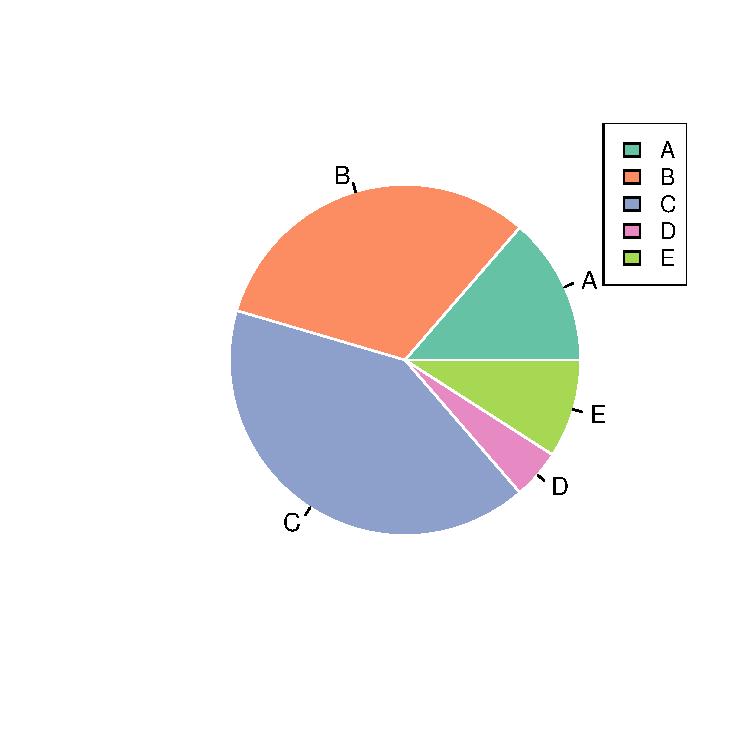
\includegraphics[width=\maxwidth]{figure/plot_pie_basic-1} 

\end{knitrout}
\clearpage
\subsubsection{Paquete ggplot2}
Una vez m\'as, se encuentra en el proyecto este paquete \cite{docu_ggplot2}
. Como se ha comprobado antes este paquete es muy vers\'atil para crear los diagramas ofreciendo muy buena personalizaci\'on.~\\
Para la realizaci\'on de estos diagramas circulares la funci\'on \texttt{coord polar} ha resultado ser muy \'util y esta vez, al igual que en el diagrama de barras radiales, se va a transformar la Y de forma lineal a radial, pero la diferencia con aquel diagrama es que al dejar el eje X sin asignar cambia del diagrama de barras radiales al de sectores.~\\
Para ello se vuelven a preparar los datos necesarios.
\begin{knitrout}
\definecolor{shadecolor}{rgb}{0.969, 0.969, 0.969}\color{fgcolor}\begin{kframe}
\begin{alltt}
\hlkwd{library}\hlstd{(ggplot2)}
\hlstd{data} \hlkwb{<-} \hlkwd{data.frame}\hlstd{(}
  \hlkwc{group}\hlstd{=LETTERS[}\hlnum{1}\hlopt{:}\hlnum{5}\hlstd{],}
  \hlkwc{value}\hlstd{=}\hlkwd{c}\hlstd{(}\hlnum{13}\hlstd{,}\hlnum{7}\hlstd{,}\hlnum{9}\hlstd{,}\hlnum{21}\hlstd{,}\hlnum{2}\hlstd{)}
\hlstd{)}
\end{alltt}
\end{kframe}
\end{knitrout}
El problema de este diagrama con respecto a otros que usan \texttt{ggplot2} es la posicion de las etiquetas ya que solo con la funci\'on \texttt{geom label} no situa las etiquetas en su correcto lugar, por lo que hay que preparar el texto para ello.
\begin{knitrout}
\definecolor{shadecolor}{rgb}{0.969, 0.969, 0.969}\color{fgcolor}\begin{kframe}
\begin{alltt}
\hlkwd{library}\hlstd{(tidyverse)}
\hlstd{data} \hlkwb{<-} \hlstd{data} \hlopt
  \hlkwd{arrange}\hlstd{(}\hlkwd{desc}\hlstd{(group))} \hlopt
  \hlkwd{mutate}\hlstd{(}\hlkwc{Porcentaje} \hlstd{= value} \hlopt{/} \hlkwd{sum}\hlstd{(data}\hlopt{$}\hlstd{value)} \hlopt{*}\hlnum{100}\hlstd{)} \hlopt
  \hlkwd{mutate}\hlstd{(}\hlkwc{ypos} \hlstd{=} \hlkwd{cumsum}\hlstd{(Porcentaje)}\hlopt{-} \hlnum{0.5}\hlopt{*}\hlstd{Porcentaje )}
\end{alltt}
\end{kframe}
\end{knitrout}

Y ahora se procede a la representaci\'on del gr\'afico, pasando como par\'ametros los datos a usar y asignando al eje X nada (como se dijo antes), al eje Y el procentaje. Los colores se obtienen en funci\'on del grupo. Se usa la figura geom\'etrica de la barra para representar los datos y se convierte el eje Y de lineal a radial.
\begin{knitrout}
\definecolor{shadecolor}{rgb}{0.969, 0.969, 0.969}\color{fgcolor}\begin{kframe}
\begin{alltt}
\hlkwd{ggplot}(data, \hlkwd{aes}(x=\hlstr{""}, y=Porcentaje, fill=group)) +
  \hlkwd{geom_bar}(stat=\hlstr{"identity"}, width=1, color=\hlstr{"white"}) +
  \hlkwd{coord_polar}(\hlstr{"y"}, start=0) +
  \hlkwd{theme_void}() + 
  \hlkwd{theme}(legend.position=\hlstr{"none"}) +
\end{alltt}
\end{kframe}
\end{knitrout}
Se coloca el texto en la posici\'on anteriormente calculada y se ajusta la paleta de colores con el paquete usado antes.
\begin{knitrout}
\definecolor{shadecolor}{rgb}{0.969, 0.969, 0.969}\color{fgcolor}\begin{kframe}
\begin{alltt}
  \hlkwd{geom_text}\hlstd{(}\hlkwd{aes}\hlstd{(}\hlkwc{y} \hlstd{= ypos,} \hlkwc{label} \hlstd{= group),} \hlkwc{color} \hlstd{=} \hlstr{"white"}\hlstd{,} \hlkwc{size}\hlstd{=}\hlnum{5}\hlstd{)} \hlopt{+}
  \hlkwd{scale_fill_brewer}\hlstd{(}\hlkwc{palette}\hlstd{=}\hlstr{"Set1"}\hlstd{)}
\end{alltt}
\end{kframe}
\end{knitrout}
\clearpage
Y as\'i resulta el gr\'afico.
\begin{knitrout}
\definecolor{shadecolor}{rgb}{0.969, 0.969, 0.969}\color{fgcolor}

{\centering 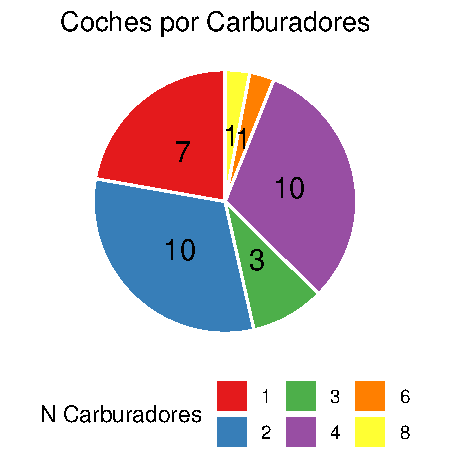
\includegraphics[width=\maxwidth]{figure/plot_ggplot_pie-1} 

}



\end{knitrout}
\begin{center}
\textbf{. . .}
\end{center}
~\\
Al igual que muchos de los gr\'aficos que usan ggplot2, se puede crear con el paquete ggiraph \cite{docu_ggiraph}
los gr\'aficos de ggplot2 interactivos, con la sustituci\'on de la funci\'on que implemente los sectores por sus variante interactiva, en este caso \texttt{geom-col-interactive}.
\begin{knitrout}
\definecolor{shadecolor}{rgb}{0.969, 0.969, 0.969}\color{fgcolor}\begin{kframe}
\begin{alltt}
\hlkwd{library}\hlstd{(ggiraph)}
\hlstd{p} \hlkwb{<-} \hlkwd{ggplot}\hlstd{(data,} \hlkwd{aes}\hlstd{(}\hlkwc{x}\hlstd{=}\hlstr{""}\hlstd{,} \hlkwc{y}\hlstd{=value,} \hlkwc{fill}\hlstd{=group,} \hlkwc{tooltip} \hlstd{= group,} \hlkwc{data_id} \hlstd{= group))} \hlopt{+}
  \hlkwd{geom_col_interactive}\hlstd{()} \hlopt{+}
  \hlkwd{coord_polar}\hlstd{(}\hlstr{"y"}\hlstd{,} \hlkwc{start}\hlstd{=}\hlnum{0}\hlstd{)} \hlopt{+}
  \hlkwd{theme_void}\hlstd{()} \hlopt{+}
  \hlkwd{theme}\hlstd{(}\hlkwc{legend.position} \hlstd{=} \hlstr{"none"}\hlstd{)}
\hlkwd{girafe}\hlstd{(}\hlkwc{ggobj} \hlstd{= p)}
\end{alltt}
\end{kframe}
\end{knitrout}
\vbox{
    \centering
    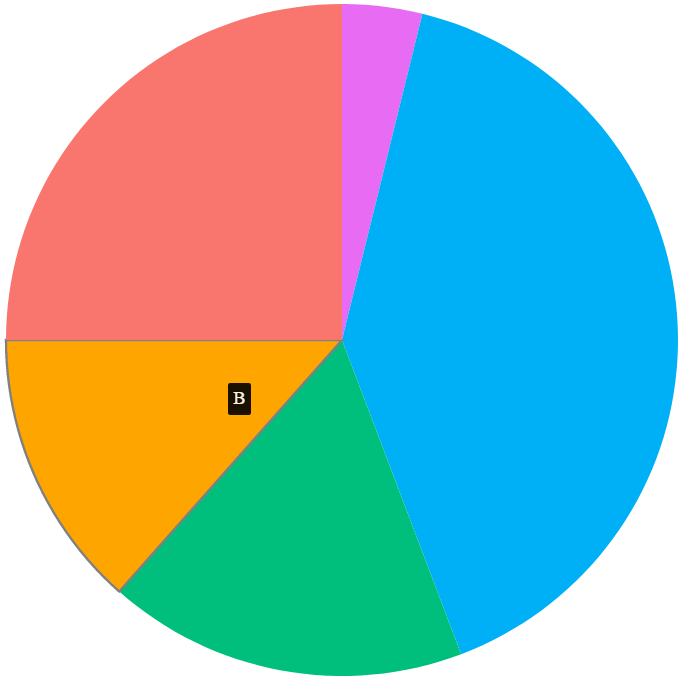
\includegraphics[width=0.4\textwidth]{imag/pie_ggplot2}
}
\clearpage
\subsubsection{Paquete plotrix}
Este paquete \cite{docu_plotrix} 
tiene dos posibles formas de representar los diagramas de sectores, una en 2D y otra en 3D. Esto no lo tiene ning\'un otro paquete que se haya investigado en este proyecto.~\\~\\
Primero se ver\'a la forma de representar el gr\'afico en 2D. Para ello se usa la funci\'on \texttt{floating.pie} y \texttt{pie.labels} para las etiquetas. Se obtienen los datos de los valores anteriores al igual que las etiquetas pero, para que el gr\'afico resulte algo distinto, tambi\'en se va a usar el par\'ametro \texttt{explode}.

Para ello se necesita la libreria y crear un espacio para luego realizar los sectores.
\begin{knitrout}
\definecolor{shadecolor}{rgb}{0.969, 0.969, 0.969}\color{fgcolor}\begin{kframe}
\begin{alltt}
\hlkwd{library}\hlstd{(plotrix)}
\hlkwd{plot}\hlstd{(}\hlnum{0}\hlstd{,}\hlkwc{xlim}\hlstd{=}\hlkwd{c}\hlstd{(}\hlnum{1.5}\hlstd{,}\hlnum{5}\hlstd{),}\hlkwc{ylim}\hlstd{=}\hlkwd{c}\hlstd{(}\hlnum{1}\hlstd{,}\hlnum{5}\hlstd{),}\hlkwc{type}\hlstd{=}\hlstr{"n"}\hlstd{,}\hlkwc{axes}\hlstd{=}\hlnum{FALSE}\hlstd{,}\hlkwc{xlab}\hlstd{=}\hlstr{""}\hlstd{,}\hlkwc{ylab}\hlstd{=}\hlstr{""}\hlstd{,} \hlkwc{main} \hlstd{=} \hlstr{"2D"}\hlstd{)}
\end{alltt}
\end{kframe}
\end{knitrout}
Luego para las etiquetas se calculan las posiciones y \'angulos donde deben estar, proporcionados ya la por funci\'on \texttt{floating.pie}.
\begin{knitrout}
\definecolor{shadecolor}{rgb}{0.969, 0.969, 0.969}\color{fgcolor}\begin{kframe}
\begin{alltt}
\hlstd{angulos} \hlkwb{<-} \hlkwd{floating.pie}\hlstd{(}\hlnum{3.25}\hlstd{,} \hlnum{3}\hlstd{, data}\hlopt{$}\hlstd{value,} \hlkwc{radius} \hlstd{=} \hlnum{1.5}\hlstd{,}
                        \hlkwc{col} \hlstd{=} \hlkwd{c}\hlstd{(}\hlstr{"#ff0000"}\hlstd{,}\hlstr{"#80ff00"}\hlstd{,}\hlstr{"#00ffff"}\hlstd{,}\hlstr{"#44bbff"}\hlstd{,}\hlstr{"#8000ff"}\hlstd{))}
\end{alltt}
\end{kframe}
\end{knitrout}
Y para las etiquetas \texttt{pie.labels} necesita dichos angulos, la posici\'on del centro del diagrama y las etiquetas.
\begin{knitrout}
\definecolor{shadecolor}{rgb}{0.969, 0.969, 0.969}\color{fgcolor}\begin{kframe}
\begin{alltt}
\hlkwd{pie.labels}\hlstd{(}\hlnum{3.25}\hlstd{,} \hlnum{3}\hlstd{, angulos, data}\hlopt{$}\hlstd{group,} \hlkwc{minangle} \hlstd{=} \hlnum{0.2}\hlstd{,} \hlkwc{radius} \hlstd{=} \hlnum{1.6}\hlstd{)}
\end{alltt}
\end{kframe}
\end{knitrout}
Despu\'es se realiza el mismo trabajo para el par\'ametro \texttt{explode}, pero incluyendo el vector con las distancias al centro (tanto en el gr\'afico como en las etiquetas).
\begin{knitrout}
\definecolor{shadecolor}{rgb}{0.969, 0.969, 0.969}\color{fgcolor}\begin{kframe}
\begin{alltt}
\hlkwd{pie.labels}\hlstd{(}\hlnum{3.25}\hlstd{,} \hlnum{3}\hlstd{, angulos, data}\hlopt{$}\hlstd{group,} \hlkwc{minangle} \hlstd{=} \hlnum{0.2}\hlstd{,} \hlkwc{radius} \hlstd{=} \hlnum{1.6}\hlstd{)}
\hlkwd{plot}\hlstd{(}\hlnum{0}\hlstd{,}\hlkwc{xlim}\hlstd{=}\hlkwd{c}\hlstd{(}\hlnum{1.5}\hlstd{,}\hlnum{5}\hlstd{),}\hlkwc{ylim}\hlstd{=}\hlkwd{c}\hlstd{(}\hlnum{1}\hlstd{,}\hlnum{5}\hlstd{),}\hlkwc{type}\hlstd{=}\hlstr{"n"}\hlstd{,}\hlkwc{axes}\hlstd{=}\hlnum{FALSE}\hlstd{,}\hlkwc{xlab}\hlstd{=}\hlstr{""}\hlstd{,}\hlkwc{ylab}\hlstd{=}\hlstr{""}\hlstd{,} \hlkwc{main} \hlstd{=} \hlstr{"2D Explode"}\hlstd{)}
\hlstd{angulos} \hlkwb{<-} \hlkwd{floating.pie}\hlstd{(}\hlnum{3.25}\hlstd{,} \hlnum{3}\hlstd{, data}\hlopt{$}\hlstd{value,} \hlkwc{radius} \hlstd{=} \hlnum{1.5}\hlstd{,}
                        \hlkwc{col} \hlstd{=} \hlkwd{c}\hlstd{(}\hlstr{"#ff0000"}\hlstd{,}\hlstr{"#80ff00"}\hlstd{,}\hlstr{"#00ffff"}\hlstd{,}\hlstr{"#44bbff"}\hlstd{,}\hlstr{"#8000ff"}\hlstd{),}
                        \hlkwc{explode} \hlstd{=} \hlkwd{c}\hlstd{(}\hlnum{0.2}\hlstd{,}\hlnum{0}\hlstd{,}\hlnum{0.1}\hlstd{,}\hlnum{0.2}\hlstd{,}\hlnum{0}\hlstd{))}
\hlkwd{pie.labels}\hlstd{(}\hlnum{3.25}\hlstd{,} \hlnum{3}\hlstd{, angulos, data}\hlopt{$}\hlstd{group,} \hlkwc{minangle} \hlstd{=} \hlnum{0.2}\hlstd{,} \hlkwc{radius} \hlstd{=} \hlnum{1.6}\hlstd{,}
           \hlkwc{explode} \hlstd{=} \hlkwd{c}\hlstd{(}\hlnum{0.2}\hlstd{,}\hlnum{0}\hlstd{,}\hlnum{0.1}\hlstd{,}\hlnum{0.2}\hlstd{,}\hlnum{0}\hlstd{))}
\end{alltt}
\end{kframe}
\end{knitrout}
\begin{knitrout}
\definecolor{shadecolor}{rgb}{0.969, 0.969, 0.969}\color{fgcolor}

{\centering 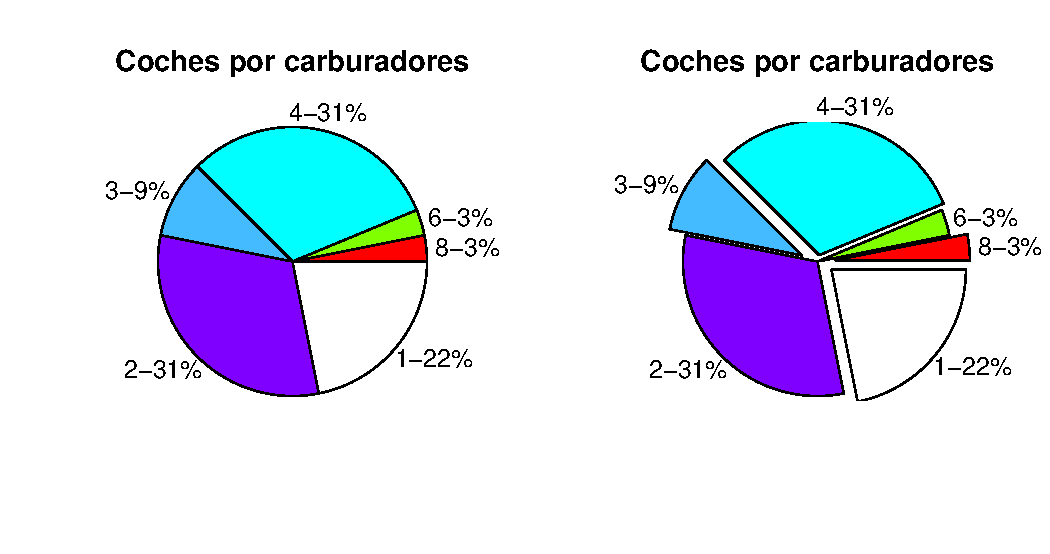
\includegraphics[width=\maxwidth]{figure/plot_plotrix_2D-1} 

}



\end{knitrout}
Y, por \'ultimo, se realiza el mismo gr\'afico pero en 3D, gracias a la funci\'on \texttt{pie3D}. Esta forma requiere guardar el resultado en, por ejemplo, png.~\\

Para ello se establece el nombre del archivo.
\begin{knitrout}
\definecolor{shadecolor}{rgb}{0.969, 0.969, 0.969}\color{fgcolor}\begin{kframe}
\begin{alltt}
\hlkwd{png}\hlstd{(}\hlkwc{file} \hlstd{=} \hlstr{"3d_sectores.png"}\hlstd{)}
\end{alltt}
\end{kframe}
\end{knitrout}
Y crear el gr\'afico con los valores iguales que antes.
\begin{knitrout}
\definecolor{shadecolor}{rgb}{0.969, 0.969, 0.969}\color{fgcolor}\begin{kframe}
\begin{alltt}
\hlkwd{pie3D}\hlstd{(data}\hlopt{$}\hlstd{value,} \hlkwc{labels} \hlstd{= data}\hlopt{$}\hlstd{group,} \hlkwc{explode} \hlstd{=} \hlnum{0.1}\hlstd{,} \hlkwc{main} \hlstd{=} \hlstr{"Sectores 3D"}\hlstd{,}
      \hlkwc{col}\hlstd{=}\hlkwd{c}\hlstd{(}\hlstr{"#ff0000"}\hlstd{,}\hlstr{"#80ff00"}\hlstd{,}\hlstr{"#00ffff"}\hlstd{,}\hlstr{"#44bbff"}\hlstd{,}\hlstr{"#8000ff"}\hlstd{))}
\end{alltt}
\end{kframe}
\end{knitrout}
 Y al final guardarlo, resultando en el siguiente gr\'afico.
\begin{knitrout}
\definecolor{shadecolor}{rgb}{0.969, 0.969, 0.969}\color{fgcolor}\begin{kframe}
\begin{alltt}
\hlkwd{dev.off}\hlstd{()}
\end{alltt}
\end{kframe}
\end{knitrout}

\vbox{
    \centering
    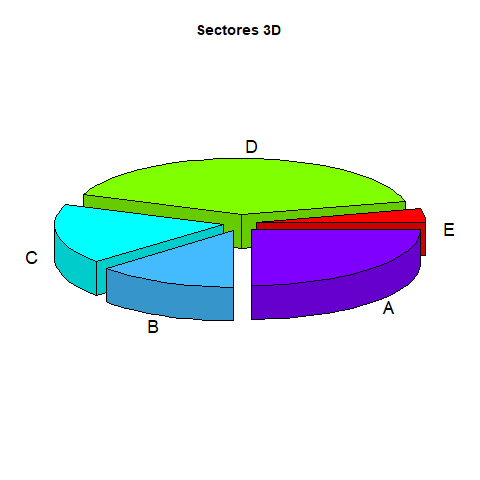
\includegraphics[width=0.4\textwidth]{imag/3d_sectores}
}
\begin{center}
\textbf{. . .}
\end{center}
\subsubsection{Paquete rCharts}
Tanto en este paquete como en el siguiente se van a traer unos diagramas de sectores interactivos. Al optar por el formato del papel y no p\'agina web en este trabajo, se procede al final de cada paquete a mostrar la forma de guardar los gr\'aficos en html para su posterior visualizaci\'on.~\\
Este paquete \cite{docu_rcharts} 
sirve para crear y personalizar gr\'aficos interactivos en javascript transformandolos a partir de R. Para representar este gr\'afico se va a reutilizar los mismos valores que antes e implementarlos con la funci\'on \texttt{nPlot}.
\begin{knitrout}
\definecolor{shadecolor}{rgb}{0.969, 0.969, 0.969}\color{fgcolor}\begin{kframe}
\begin{alltt}
\hlkwd{library}\hlstd{(rCharts)}
\hlstd{p} \hlkwb{<-} \hlkwd{nPlot}\hlstd{(value}\hlopt{~}\hlstd{group,} \hlkwc{data} \hlstd{= data,} \hlkwc{type} \hlstd{=} \hlstr{'pieChart'}\hlstd{)}
\end{alltt}
\end{kframe}
\end{knitrout}
El problema viene a la hora de mostrarlo ya que p es una script de javascripts, por lo que para mostrarse con interactividad se necesita incluir en una pagina html. Para ello, este gr\'afico solo necesita de la etiqueta \texttt{<html>} al principio y \texttt{</html>} al final, copiando el script del resultado de la siguiente orden.
\begin{knitrout}
\definecolor{shadecolor}{rgb}{0.969, 0.969, 0.969}\color{fgcolor}\begin{kframe}
\begin{alltt}
\hlstd{p}\hlopt{$}\hlkwd{print}\hlstd{(}\hlkwc{include_assets}\hlstd{=T)}
\end{alltt}
\end{kframe}
\end{knitrout}
Dando como resultado la siguiente imagen como p\'agina web.~\\
\vbox{
    \centering
    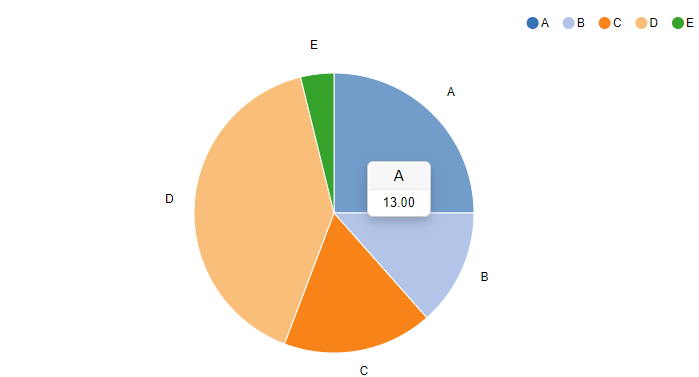
\includegraphics[width=0.7\textwidth]{imag/sectores_rcharts}
}
\begin{center}
\textbf{. . .}
\end{center}
\subsubsection{Paquete plotly}
Este paquete \cite{docu_plotly} 
se dedica principalmente a crear gr\'aficos interactivos, de los gr\'aficos m\'as comunes y otros m\'as espec\'ificos que se ver\'an mas adelante. Por ello  no se visualiza el gr\'afico resultante sino una foto de \'el.~\\
Para realizarlo plotly ofrece la funci\'on \texttt{plot-ly}, b\'asica para cualquier plot con este paquete, si se le da el tipo pie reproduce el diagrama deseado. Como hasta ahora se va a seguir utilizando los mismos datos.
\begin{knitrout}
\definecolor{shadecolor}{rgb}{0.969, 0.969, 0.969}\color{fgcolor}\begin{kframe}
\begin{alltt}
\hlkwd{library}\hlstd{(plotly)}
\hlstd{p} \hlkwb{<-} \hlkwd{plot_ly}\hlstd{(data,} \hlkwc{labels} \hlstd{= data}\hlopt{$}\hlstd{group,} \hlkwc{values} \hlstd{= data}\hlopt{$}\hlstd{value,} \hlkwc{type} \hlstd{=} \hlstr{'pie'}\hlstd{)} \hlopt
  \hlkwd{layout}\hlstd{(}\hlkwc{title} \hlstd{=} \hlstr{'Plotly'}\hlstd{,}
         \hlkwc{xaxis} \hlstd{=} \hlkwd{list}\hlstd{(}\hlkwc{showgrid} \hlstd{=} \hlnum{FALSE}\hlstd{,} \hlkwc{zeroline} \hlstd{=} \hlnum{FALSE}\hlstd{,} \hlkwc{showticklabels} \hlstd{=} \hlnum{FALSE}\hlstd{),}
         \hlkwc{yaxis} \hlstd{=} \hlkwd{list}\hlstd{(}\hlkwc{showgrid} \hlstd{=} \hlnum{FALSE}\hlstd{,} \hlkwc{zeroline} \hlstd{=} \hlnum{FALSE}\hlstd{,} \hlkwc{showticklabels} \hlstd{=} \hlnum{FALSE}\hlstd{))}
\end{alltt}
\end{kframe}
\end{knitrout}
Aunque esta vez la forma de guardarlo en una p\'agina web, es mucho mas sencilla gracias al paquete \texttt{htmlwidgets}, mediante la siguiente orden.
\begin{knitrout}
\definecolor{shadecolor}{rgb}{0.969, 0.969, 0.969}\color{fgcolor}\begin{kframe}
\begin{alltt}
\hlkwd{library}\hlstd{(htmlwidgets)}
\hlkwd{saveWidget}\hlstd{(p,} \hlkwc{file} \hlstd{=} \hlstr{"plotly_pie.html"}\hlstd{)}
\end{alltt}
\end{kframe}
\end{knitrout}
Resultando en el siguiente grafo (no interactivo salvo en el html).~\\
\vbox{
    \centering
    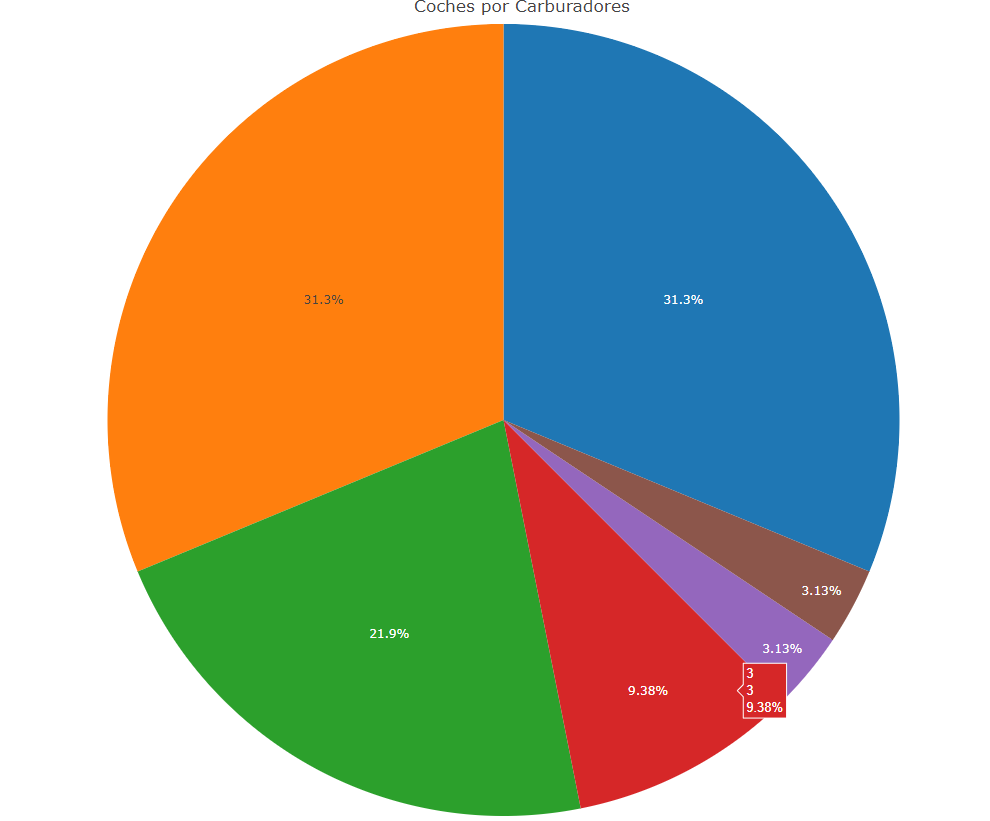
\includegraphics[width=0.4\textwidth]{imag/plotly_pie}
}
\subsubsection{Paquete ggiraphExtra}
Este paquete \cite{docu_ggiraphExtra} 
es una extensi\'on del paquete \texttt{ggiraph}, creando sus propias funciones al haber sustituido las variantes interactivas de las funciones de \texttt{ggplot2} con las funciones de \texttt{ggiraph}. Por lo que otra forma de crear un diagrama de sectores interactivo es mediante este paquete. Si se requiere el uso de funciones de ggplot2, el gr\'afico pierde interactividad y pasa a ser un paquete ayudante de ggplot2.~\\
Para la comparaci\'on entre paquetes se opta por el uso de los datos ya usados anteriormente. 
\begin{knitrout}
\definecolor{shadecolor}{rgb}{0.969, 0.969, 0.969}\color{fgcolor}\begin{kframe}
\begin{alltt}
\hlkwd{library}\hlstd{(ggiraphExtra)}
\hlkwd{ggPie}\hlstd{(data,} \hlkwd{aes}\hlstd{(} \hlkwc{pies}\hlstd{=group,} \hlkwc{count}\hlstd{=value),} \hlkwc{interactive} \hlstd{=} \hlnum{TRUE}\hlstd{)}
\end{alltt}
\end{kframe}
\end{knitrout}
\vbox{
    \centering
    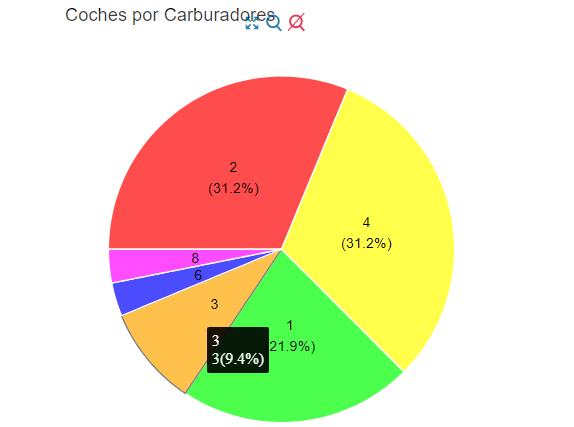
\includegraphics[width=0.4\textwidth]{imag/pir_ggiraph}
}
\begin{center}
\textbf{. . .}
\end{center}
\subsubsection{Comparaciones}
Este diagrama es uno de los dos que se pueden crear mediante el uso del lenguaje R sin ning\'un paquete adicional pero, aunque el gr\'afico resultante es correcto, no tiene ninguna forma de personalizaci\'on. Con \texttt{ggplot2} ofrece el mismo buen resultado que todas las veces que se usa, ofreciendo un gr\'afico que cumple su misi\'on adem\'as de ofrecer gran capacidad de personalizaci\'on. En este diagrama el paquete \texttt{ggiraph} ofrece una ayuda al paquete ggplot2 a\~nadiendo el componente de interactividad.~\\ Otro paquete que ofrece una funci\'on interesante dentro de este diagrama es \texttt{plotrix}, con el cual, aparte de crear un gr\'afico adecuado, con personalizaci\'on (de dificil apredizaje a la hora de crearlo comparado con los dem\'as paquetes encontrados), se a\~nade la funci\'on de crear el diagrama de sectores en 3D.~\\
Los siguientes tres paquetes que ofrecen funciones para crear el diagrama de sectores, incluyendo siempre la variable de interactividad, que ayuda a la compresi\'on de diagramas de sectores con una cantidad de datos mayor de los normal son: \texttt{Rcharts} que crea el diagrama con su funci\'on predeterminada, aumentando su facilidad de aprendizaje, especificando que el tipo de diagrama que se requiere es el de sectores. \texttt{Plotly} al igual que rcharts puede crear el diagrama solo con su funci\'on principal especificando su tipo, pero a la hora de personalizaci\'on proporciona m\'as variantes que el paquete anterior, a\~nadiendo mas funciones al estilo que lo hace \texttt{ggplot2}. Con \texttt{ggiraphExtra} se vuelve al caso de rcharts de solo una funci\'on para representar el diagrama, pero carece de la capacidad de m\'as personalizaci\'on.~\\
En conclusi\'on, todos los paquetes encontrados para implementar el diagrama de sectores ofrecen un gr\'afico similar, salvo en la capacidad de personalizaci\'on e interactividad, pero por su sencillez prevalece la funci\'on que ofrece el lenguaje R sin paquete. Aunque, si lo que se busca es m\'as personalizaci\'on, se recomienda el uso de \texttt{ggplot2} y, si se busca interactividads se puede escoger entre \texttt{ggplot2-ggiraph} y \texttt{plotly}.
%%%%%%%%%%%%%%%%%%%%%%%%%%%%%%%%%%%%%%%%%%%%%%%%%%%%%%%%%%%%%%%%%%
\clearpage
%%%%%%%%%%%%%%%%%%%%%%%%%%%%%%%%%%%%%%%%%%%%%%%%%%%%%%%
\subsection{Diagrama de Rose of Nightingale}\label{ssec:rose}
Al recopilar las formas para realizar este diagrama se descubre que es la misma que si el diagrama constara de gr\'aficos de columnas apiladas, pero dando el formato de uni\'on entre barras que aporta el diagrama de sectores.
\subsubsection{Paquete ggplot2}
Otra vez en el proyecto se cruza este paquete \cite{docu_ggplot2} 
aportando su versatilidad. El gr\'afico consistir\'a de nuevo en crear un diagrama normal (lineal) y transformarlo con la ayuda de \texttt{coord polar}. Esta vez se realiza un gr\'afico de barras apiladas y transformar el eje X.~\\
Primero necesita los datos para crear las barras apiladas.
\begin{knitrout}
\definecolor{shadecolor}{rgb}{0.969, 0.969, 0.969}\color{fgcolor}\begin{kframe}
\begin{alltt}
\hlstd{data}\hlkwb{=}\hlkwd{read.csv}\hlstd{(}\hlstr{"rose.csv"}\hlstd{,} \hlkwc{sep} \hlstd{=} \hlstr{";"}\hlstd{)}
\hlkwd{head}\hlstd{(data)}
\end{alltt}
\begin{verbatim}
##        MES  A   B C   D E   F G
## 1  January 10   9 8   7 6   5 4
## 2 February  5 4,5 4 3,5 3 2,5 2
## 3    March  7   6 5   4 3   2 2
## 4    April  9   7 8   7 6   5 4
## 5      May 11   8 4 3,5 3 2,5 2
## 6     June 13   9 5   4 3   2 2
\end{verbatim}
\end{kframe}
\end{knitrout}
Consiste de unos valores aleatorios ordenados por grupo y mes, pero necesita datos agrupados por solo una variable que en esta vez se usan los meses. Gracias a \texttt{reshape2} se consigue el agrupamiento por mes.
\begin{knitrout}
\definecolor{shadecolor}{rgb}{0.969, 0.969, 0.969}\color{fgcolor}\begin{kframe}
\begin{alltt}
\hlkwd{library}\hlstd{(reshape2)}
\hlstd{data1}\hlkwb{=}\hlkwd{data.frame}\hlstd{(}\hlkwd{t}\hlstd{(data))}
\hlstd{data2}\hlkwb{=}\hlstd{data1[}\hlnum{2}\hlopt{:}\hlnum{8}\hlstd{,]}
\hlkwd{colnames}\hlstd{(data2)}\hlkwb{=}\hlstd{month.name}
\hlstd{data2}\hlopt{$}\hlstd{group}\hlkwb{=}\hlkwd{row.names}\hlstd{(data2)}
\hlstd{data3}\hlkwb{=}\hlkwd{melt}\hlstd{(data2,}\hlkwc{id}\hlstd{=}\hlstr{"group"}\hlstd{)}
\hlkwd{head}\hlstd{(data3)}
\end{alltt}
\begin{verbatim}
##   group variable value
## 1     A  January    10
## 2     B  January     9
## 3     C  January     8
## 4     D  January     7
## 5     E  January     6
## 6     F  January     5
\end{verbatim}
\end{kframe}
\end{knitrout}
Y ahora, para crear el gr\'afico, lo \'unico que hay que hacer es crear el diagrama de barras apiladas y aplicarle la transformaci\'on, adem\'as de la est\'etica deseada.

Para ello se llama a la funci\'on \texttt{ggplot} con los datos de data3 y asignando el eje X a los meses, el Y, a los valores y los colores en funci\'on del grupo. Y se crea el diagrama de barras tradicional con \texttt{geom-bar(stat="identity")}.
\begin{knitrout}
\definecolor{shadecolor}{rgb}{0.969, 0.969, 0.969}\color{fgcolor}\begin{kframe}
\begin{alltt}
\hlkwd{library}(ggplot2)
\hlkwd{ggplot}(data3,\hlkwd{aes}(x=variable,y=value,fill=group))+
  \hlkwd{geom_bar}(stat=\hlstr{"identity"},width=1,colour=\hlstr{"white"},size=0.1)+
\end{alltt}
\end{kframe}
\end{knitrout}
Ahora se transforma la coordenada X y se aplica la escala de colores deseada.
\begin{knitrout}
\definecolor{shadecolor}{rgb}{0.969, 0.969, 0.969}\color{fgcolor}\begin{kframe}
\begin{alltt}
  \hlkwd{coord_polar}(\hlstr{'x'})+
  \hlkwd{scale_fill_brewer}(palette=\hlstr{"Blues"})+
\end{alltt}
\end{kframe}
\end{knitrout}
Y por \'ultimo la est\'etica del grafo deseada (sin leyenda, ejes, fondo blanco, etc).
\begin{knitrout}
\definecolor{shadecolor}{rgb}{0.969, 0.969, 0.969}\color{fgcolor}\begin{kframe}
\begin{alltt}
  \hlkwd{xlab}\hlstd{(}\hlstr{""}\hlstd{)}\hlopt{+}\hlkwd{ylab}\hlstd{(}\hlstr{""}\hlstd{)} \hlopt{+}
  \hlkwd{theme_minimal}\hlstd{()} \hlopt{+}
  \hlkwd{theme}\hlstd{(}\hlkwc{legend.position} \hlstd{=} \hlstr{"none"}\hlstd{,}
        \hlkwc{axis.line} \hlstd{=} \hlkwd{element_blank}\hlstd{(),}
        \hlkwc{axis.text.y} \hlstd{=} \hlkwd{element_blank}\hlstd{(),}
        \hlkwc{axis.ticks} \hlstd{=} \hlkwd{element_blank}\hlstd{())}
\end{alltt}
\end{kframe}
\end{knitrout}
Dando como resultado el gr\'afico.
\begin{knitrout}
\definecolor{shadecolor}{rgb}{0.969, 0.969, 0.969}\color{fgcolor}

{\centering \includegraphics[width=\maxwidth]{figure/plot_rose_1-1} 

}



\end{knitrout}
\begin{center}
\textbf{. . .}
\end{center}
~\\
Ahora, para ver el gr\'afico que le da nombre al diagrama, se van a obtener los datos de la libreria \texttt{HistData} y se va a simular el grafo de Rose of Nightingale.
\begin{knitrout}
\definecolor{shadecolor}{rgb}{0.969, 0.969, 0.969}\color{fgcolor}\begin{kframe}
\begin{alltt}
\hlkwd{library}\hlstd{(HistData)}
\hlkwd{data}\hlstd{(Nightingale)}
\end{alltt}
\end{kframe}
\end{knitrout}
Como en este gr\'afico solo se muestra la fecha, las muertes y su causa, se va a tener que transformar estos datos para que se puedan mostrar al igual que el gr\'afico que se muestra en \cite[p\'ag 113]{Circle}

Primero solo se necesita la fecha y las muertes por enfermedad, heridas y otras causas y ordenarlas por la causa de la muerte al igual que en el ejemplo anterior.
\begin{knitrout}
\definecolor{shadecolor}{rgb}{0.969, 0.969, 0.969}\color{fgcolor}\begin{kframe}
\begin{alltt}
\hlkwd{require}\hlstd{(reshape)}
\hlstd{Night}\hlkwb{<-} \hlstd{Nightingale[,}\hlkwd{c}\hlstd{(}\hlnum{1}\hlstd{,}\hlnum{8}\hlopt{:}\hlnum{10}\hlstd{)]}
\hlstd{melted} \hlkwb{<-} \hlkwd{melt}\hlstd{(Night,} \hlstr{"Date"}\hlstd{)}
\hlkwd{names}\hlstd{(melted)} \hlkwb{<-} \hlkwd{c}\hlstd{(}\hlstr{"Fecha"}\hlstd{,} \hlstr{"Causa"}\hlstd{,} \hlstr{"Muertes"}\hlstd{)}
\hlstd{melted}\hlopt{$}\hlstd{Causa} \hlkwb{<-} \hlkwd{sub}\hlstd{(}\hlstr{"\textbackslash{}\textbackslash{}.rate"}\hlstd{,} \hlstr{""}\hlstd{, melted}\hlopt{$}\hlstd{Causa)}
\end{alltt}
\end{kframe}
\end{knitrout}

Luego, al igual que el gr\'afico en el libro, separa los datos para crear dos gr\'aficos, con la separaci\'on a partir de la fecha marzo de 1855.
\begin{knitrout}
\definecolor{shadecolor}{rgb}{0.969, 0.969, 0.969}\color{fgcolor}\begin{kframe}
\begin{alltt}
\hlstd{Night} \hlkwb{<-} \hlstd{melted}
\hlstd{Night}\hlopt{$}\hlstd{Month} \hlkwb{<-} \hlkwd{format}\hlstd{(Night}\hlopt{$}\hlstd{Fecha,} \hlstr{"%b %Y"}\hlstd{)}
\hlstd{Night1} \hlkwb{<-} \hlkwd{subset}\hlstd{(Night, Fecha} \hlopt{<} \hlkwd{as.Date}\hlstd{(}\hlstr{"1855-04-01"}\hlstd{))}
\hlstd{Night2} \hlkwb{<-} \hlkwd{subset}\hlstd{(Night, Fecha} \hlopt{>=} \hlkwd{as.Date}\hlstd{(}\hlstr{"1855-04-01"}\hlstd{))}
\end{alltt}
\end{kframe}
\end{knitrout}
Ahora se exponen los gr\'aficos, uno al lado del otro con la misma f\'ormula que el ejemplo anterior con el eje X las fechas, el Y las muertes y el color en funci\'on de las causas.~\\
Para realizar los diagramas se emplea el siguiente c\'odigo que no se explica porque en esencia es el ejemplo anterior.
\begin{knitrout}
\definecolor{shadecolor}{rgb}{0.969, 0.969, 0.969}\color{fgcolor}\begin{kframe}
\begin{alltt}
\hlkwd{ggplot}\hlstd{(Night1,} \hlkwd{aes}\hlstd{(}\hlkwc{x} \hlstd{=} \hlkwd{factor}\hlstd{(Fecha),} \hlkwc{y} \hlstd{= Muertes,} \hlkwc{fill} \hlstd{= Causa))} \hlopt{+}
  \hlkwd{geom_bar}\hlstd{(}\hlkwc{width} \hlstd{=} \hlnum{1}\hlstd{,} \hlkwc{stat} \hlstd{=} \hlstr{"identity"}\hlstd{,} \hlkwc{color}\hlstd{=}\hlstr{"black"}\hlstd{)} \hlopt{+}
  \hlkwd{coord_polar}\hlstd{(}\hlkwc{start} \hlstd{=} \hlnum{3}\hlopt{*}\hlstd{pi}\hlopt{/}\hlnum{2}\hlstd{)} \hlopt{+}
  \hlkwd{xlab}\hlstd{(}\hlstr{""}\hlstd{)} \hlopt{+}  \hlkwd{ylab}\hlstd{(}\hlstr{""}\hlstd{)} \hlopt{+}
  \hlkwd{scale_y_sqrt}\hlstd{()} \hlopt{+}
  \hlkwd{scale_fill_manual}\hlstd{(}\hlkwc{values} \hlstd{=} \hlkwd{c}\hlstd{(}\hlstr{"#9ac7d4"}\hlstd{,} \hlstr{"#727374"}\hlstd{,}\hlstr{"#ea8888"}\hlstd{))} \hlopt{+}
  \hlkwd{theme_minimal}\hlstd{()} \hlopt{+}
  \hlkwd{theme}\hlstd{(}\hlkwc{panel.grid.major} \hlstd{=} \hlkwd{element_blank}\hlstd{(),}
        \hlkwc{panel.grid.minor} \hlstd{=} \hlkwd{element_blank}\hlstd{(),}
        \hlkwc{axis.line} \hlstd{=} \hlkwd{element_blank}\hlstd{(),}
        \hlkwc{axis.text.y} \hlstd{=} \hlkwd{element_blank}\hlstd{(),}
        \hlkwc{axis.ticks} \hlstd{=} \hlkwd{element_blank}\hlstd{())}
\end{alltt}
\end{kframe}

{\centering \includegraphics[width=\maxwidth]{figure/plot_rose_gg-1} 

}



\end{knitrout}
\clearpage
\begin{knitrout}
\definecolor{shadecolor}{rgb}{0.969, 0.969, 0.969}\color{fgcolor}\begin{kframe}
\begin{alltt}
\hlkwd{ggplot}\hlstd{(Night2,} \hlkwd{aes}\hlstd{(}\hlkwc{x} \hlstd{=} \hlkwd{factor}\hlstd{(Fecha),} \hlkwc{y} \hlstd{= Muertes,} \hlkwc{fill} \hlstd{= Causa))} \hlopt{+}
  \hlkwd{geom_bar}\hlstd{(}\hlkwc{width} \hlstd{=} \hlnum{1}\hlstd{,} \hlkwc{stat} \hlstd{=} \hlstr{"identity"}\hlstd{,} \hlkwc{color}\hlstd{=}\hlstr{"black"}\hlstd{)} \hlopt{+}
  \hlkwd{coord_polar}\hlstd{(}\hlkwc{start} \hlstd{=} \hlnum{3}\hlopt{*}\hlstd{pi}\hlopt{/}\hlnum{2}\hlstd{)} \hlopt{+}
  \hlkwd{xlab}\hlstd{(}\hlstr{""}\hlstd{)} \hlopt{+}  \hlkwd{ylab}\hlstd{(}\hlstr{""}\hlstd{)} \hlopt{+}
  \hlkwd{scale_y_sqrt}\hlstd{()} \hlopt{+}
  \hlkwd{scale_fill_manual}\hlstd{(}\hlkwc{values} \hlstd{=} \hlkwd{c}\hlstd{(}\hlstr{"#9ac7d4"}\hlstd{,} \hlstr{"#727374"}\hlstd{,}\hlstr{"#ea8888"}\hlstd{))} \hlopt{+}
  \hlkwd{theme_minimal}\hlstd{()} \hlopt{+}
  \hlkwd{theme}\hlstd{(}\hlkwc{panel.grid.major} \hlstd{=} \hlkwd{element_blank}\hlstd{(),}
        \hlkwc{panel.grid.minor} \hlstd{=} \hlkwd{element_blank}\hlstd{(),}
        \hlkwc{axis.line} \hlstd{=} \hlkwd{element_blank}\hlstd{(),}
        \hlkwc{axis.text.y} \hlstd{=} \hlkwd{element_blank}\hlstd{(),}
        \hlkwc{axis.ticks} \hlstd{=} \hlkwd{element_blank}\hlstd{())}
\end{alltt}
\end{kframe}

{\centering \includegraphics[width=\maxwidth]{figure/plot_rose_2_gg-1} 

}



\end{knitrout}
\clearpage
Una forma de poder usar la interactividad con diagrama de ggplot2 es con ggiraph \cite{docu_ggiraph}
y en este caso la funci\'on \texttt{geom-col-interactive} en vez de \texttt{geom-bar}.
\begin{knitrout}
\definecolor{shadecolor}{rgb}{0.969, 0.969, 0.969}\color{fgcolor}\begin{kframe}
\begin{alltt}
\hlkwd{library}\hlstd{(ggiraph)}
\hlstd{p} \hlkwb{<-} \hlkwd{ggplot}\hlstd{(Night1,} \hlkwd{aes}\hlstd{(}\hlkwc{x} \hlstd{=} \hlkwd{factor}\hlstd{(Fecha),} \hlkwc{y} \hlstd{= Muertes,} \hlkwc{fill} \hlstd{= Causa,} \hlkwc{tooltip}\hlstd{=Causa,}
                        \hlkwc{data_id} \hlstd{=}\hlkwd{factor}\hlstd{(Fecha)))} \hlopt{+}
  \hlkwd{geom_col_interactive}\hlstd{()} \hlopt{+}
  \hlkwd{coord_polar}\hlstd{(}\hlkwc{start} \hlstd{=} \hlnum{3}\hlopt{*}\hlstd{pi}\hlopt{/}\hlnum{2}\hlstd{)} \hlopt{+}
  \hlkwd{xlab}\hlstd{(}\hlstr{""}\hlstd{)} \hlopt{+}  \hlkwd{ylab}\hlstd{(}\hlstr{""}\hlstd{)} \hlopt{+}
  \hlkwd{scale_y_sqrt}\hlstd{()} \hlopt{+}
  \hlkwd{scale_fill_manual}\hlstd{(}\hlkwc{values} \hlstd{=} \hlkwd{c}\hlstd{(}\hlstr{"#9ac7d4"}\hlstd{,} \hlstr{"#727374"}\hlstd{,}\hlstr{"#ea8888"}\hlstd{))} \hlopt{+}
  \hlkwd{theme_minimal}\hlstd{()} \hlopt{+}
  \hlkwd{theme}\hlstd{(}\hlkwc{legend.position} \hlstd{=} \hlstr{"none"}\hlstd{,}
        \hlkwc{panel.grid.major} \hlstd{=} \hlkwd{element_blank}\hlstd{(),}
        \hlkwc{panel.grid.minor} \hlstd{=} \hlkwd{element_blank}\hlstd{(),}
        \hlkwc{axis.line} \hlstd{=} \hlkwd{element_blank}\hlstd{(),}
        \hlkwc{axis.text.y} \hlstd{=} \hlkwd{element_blank}\hlstd{(),}
        \hlkwc{axis.ticks} \hlstd{=} \hlkwd{element_blank}\hlstd{())}
\hlkwd{girafe}\hlstd{(}\hlkwc{ggobj} \hlstd{= p)}
\end{alltt}
\end{kframe}
\end{knitrout}
\vbox{
    \centering
    \includegraphics[width=0.6\textwidth]{imag/ggplot2_inte_rose}
}
\clearpage
\subsubsection{Paquete ggiraphExtra}
Este paquete \cite{docu_ggiraphExtra}
permite crear gr\'aficos interactivos a partir de los gr\'aficos de ggplot2. El propio paquete tiene un dataframe llamado Rose con datos para este diagrama.~\\
Una de las dos funciones que permite realizar esto es \texttt{ggRose} y necesita de los datos, la est\'etica, la paleta de color, etc.~\\
Primero se va a representar sin interartividad, para el formato de papel, pero, a continuaci\'on, se muestra la forma de pasarlo a html para la interactividad.
\begin{knitrout}
\definecolor{shadecolor}{rgb}{0.969, 0.969, 0.969}\color{fgcolor}\begin{kframe}
\begin{alltt}
\hlkwd{library}\hlstd{(ggiraphExtra)}
\hlkwd{ggRose}\hlstd{(rose,}\hlkwd{aes}\hlstd{(}\hlkwc{x}\hlstd{=Month,}\hlkwc{fill}\hlstd{=group,}\hlkwc{y}\hlstd{=value),}\hlkwc{stat}\hlstd{=}\hlstr{"identity"}\hlstd{,}\hlkwc{interactive}\hlstd{=}\hlnum{FALSE}
       \hlstd{,} \hlkwc{palette} \hlstd{=} \hlstr{"Blues"}\hlstd{)} \hlopt{+}
   \hlkwd{xlab}\hlstd{(}\hlstr{""}\hlstd{)} \hlopt{+}  \hlkwd{ylab}\hlstd{(}\hlstr{""}\hlstd{)} \hlopt{+}
  \hlkwd{scale_y_sqrt}\hlstd{()} \hlopt{+}
  \hlkwd{theme_minimal}\hlstd{()} \hlopt{+}
  \hlkwd{theme}\hlstd{(}\hlkwc{panel.grid.major} \hlstd{=} \hlkwd{element_blank}\hlstd{(),}
        \hlkwc{panel.grid.minor} \hlstd{=} \hlkwd{element_blank}\hlstd{(),}
        \hlkwc{axis.line} \hlstd{=} \hlkwd{element_blank}\hlstd{(),}
        \hlkwc{axis.text.y} \hlstd{=} \hlkwd{element_blank}\hlstd{(),}
        \hlkwc{axis.ticks} \hlstd{=} \hlkwd{element_blank}\hlstd{())}
\end{alltt}
\end{kframe}

{\centering \includegraphics[width=\maxwidth]{figure/plot_rose_ggiraph-1} 

}



\end{knitrout}
\begin{knitrout}
\definecolor{shadecolor}{rgb}{0.969, 0.969, 0.969}\color{fgcolor}\begin{kframe}
\begin{alltt}
\hlstd{p} \hlkwb{<-} \hlkwd{ggRose}\hlstd{(rose,}\hlkwd{aes}\hlstd{(}\hlkwc{x}\hlstd{=Month,}\hlkwc{fill}\hlstd{=group,}\hlkwc{y}\hlstd{=value),}\hlkwc{stat}\hlstd{=}\hlstr{"identity"}\hlstd{,}\hlkwc{interactive}\hlstd{=}\hlnum{TRUE}
       \hlstd{,} \hlkwc{palette} \hlstd{=} \hlstr{"Blues"}\hlstd{)}
\hlkwd{library}\hlstd{(htmlwidgets)}
\hlkwd{saveWidget}\hlstd{(p,} \hlkwc{file} \hlstd{=} \hlstr{"rose_interactive.html"}\hlstd{)}
\end{alltt}
\end{kframe}
\end{knitrout}
\clearpage
Otro m\'etodo para realizar el mismo diagrama es \texttt{ggBar}. Como con el paquete ggplot2 lo que se realiza es un diagrama de columnas apiladas tradicional transformando la coordenada X de lineal a radial. Como antes con la interactividad desactivada pero con la forma de verlo en html.
\begin{knitrout}
\definecolor{shadecolor}{rgb}{0.969, 0.969, 0.969}\color{fgcolor}\begin{kframe}
\begin{alltt}
\hlkwd{ggBar}\hlstd{(rose,}\hlkwd{aes}\hlstd{(}\hlkwc{x}\hlstd{=Month,}\hlkwc{fill}\hlstd{=group,}\hlkwc{y}\hlstd{=value),}\hlkwc{stat}\hlstd{=}\hlstr{"identity"}\hlstd{,}\hlkwc{polar}\hlstd{=}\hlnum{TRUE}\hlstd{,}\hlkwc{palette}\hlstd{=}\hlstr{"Blues"}
      \hlstd{,}\hlkwc{width}\hlstd{=}\hlnum{1}\hlstd{,} \hlkwc{color}\hlstd{=}\hlstr{"black"}\hlstd{,}\hlkwc{size}\hlstd{=}\hlnum{0.1}\hlstd{,}\hlkwc{reverse}\hlstd{=}\hlnum{TRUE}\hlstd{,}\hlkwc{interactive}\hlstd{=}\hlnum{FALSE}\hlstd{)}\hlopt{+}
    \hlkwd{xlab}\hlstd{(}\hlstr{""}\hlstd{)} \hlopt{+}  \hlkwd{ylab}\hlstd{(}\hlstr{""}\hlstd{)} \hlopt{+}
    \hlkwd{scale_y_sqrt}\hlstd{()} \hlopt{+}
    \hlkwd{theme_minimal}\hlstd{()} \hlopt{+}
    \hlkwd{theme}\hlstd{(}\hlkwc{panel.grid.major} \hlstd{=} \hlkwd{element_blank}\hlstd{(),}
          \hlkwc{panel.grid.minor} \hlstd{=} \hlkwd{element_blank}\hlstd{(),}
          \hlkwc{axis.line} \hlstd{=} \hlkwd{element_blank}\hlstd{(),}
          \hlkwc{axis.text.y} \hlstd{=} \hlkwd{element_blank}\hlstd{(),}
          \hlkwc{axis.ticks} \hlstd{=} \hlkwd{element_blank}\hlstd{())}
\end{alltt}
\end{kframe}

{\centering \includegraphics[width=\maxwidth]{figure/plot_bar_rose-1} 

}


\begin{kframe}\begin{alltt}
\hlstd{p} \hlkwb{<-} \hlkwd{ggBar}\hlstd{(rose,}\hlkwd{aes}\hlstd{(}\hlkwc{x}\hlstd{=Month,}\hlkwc{fill}\hlstd{=group,}\hlkwc{y}\hlstd{=value),}\hlkwc{stat}\hlstd{=}\hlstr{"identity"}\hlstd{,}\hlkwc{polar}\hlstd{=}\hlnum{TRUE}\hlstd{,}\hlkwc{palette}\hlstd{=}\hlstr{"Blues"}
      \hlstd{,}\hlkwc{width}\hlstd{=}\hlnum{1}\hlstd{,} \hlkwc{color}\hlstd{=}\hlstr{"black"}\hlstd{,}\hlkwc{size}\hlstd{=}\hlnum{0.1}\hlstd{,}\hlkwc{reverse}\hlstd{=}\hlnum{TRUE}\hlstd{,}\hlkwc{interactive}\hlstd{=}\hlnum{TRUE}\hlstd{)}
\hlkwd{library}\hlstd{(htmlwidgets)}
\hlkwd{saveWidget}\hlstd{(p,} \hlkwc{file} \hlstd{=} \hlstr{"rose2_interactive.html"}\hlstd{)}
\end{alltt}
\end{kframe}
\end{knitrout}
\begin{center}
\textbf{. . .}
\end{center}
\subsubsection{Comparaciones}
Para este diagrama se han encontrados dos paquetes, pero que en realidad es solo \texttt{ggplot2} ya que \texttt{ggiraphExtra} es un paquete que extiende la capacidad interactiva de las funciones de ggplot2. Los dos paquetes, al estar basados en el mismo, ofrecen el mismo diagrama diferenciandose con el fator de interactividad. Los dos parten de una mezcla de diagrama de barras apiladas y diagrama de sectores, por lo que cualquiera de los dos paquetes ser\'ia una buena opci\'on para implementar el diagrama de Rose of Nightingale. Ya que si se le suma el paquete \texttt{ggiraph} a ggplot2 se tendr\'ia el mismo diagrama interactivo qu\'e el que resulta del segundo paquete.
%%%%%%%%%%%%%%%%%%%%%%%%%%%%%%%%%%%%%%%%%%%%%%%%%%%%%%%%%%%%%%%%%%
\clearpage
%%%%%%%%%%%%%%%%%%%%%%%%%%%%%%%%%%%%%%%%%%%%%%%%%%%%%%%
\subsection{Diagrama de Cuadr\'icula Circular Ordenada}\label{ssec:ord}
Para este diagrama, al consistir en crear una cuadr\'icula ordenada, es necesario buscar un paquete que permita crear ese tipos de diagramas y pueda incluir en cada celda alg\'un tipo de gr\'afico, imagenes, texto, etc. El \'unico paquete que permite hacer eso es \texttt{circlize}.
\subsubsection{Paquete circlize}
Se vuelve a ver este paquete \cite{docu_circlize}
en el trabajo y, como se ha visto en otras ocasiones, dentro de este paquete existe una funci\'on que permite crear las celdas y, dentro de ellas implementar distintos gr\'aficos, con cada una de las funciones que permiten crearlos.~\\
Lo primero es crear dichas celdas con la funci\'on \texttt{circos.track}. Esta funci\'on crea las celdas divididas por anillos empezando de exterior a interior y, para dividir cada anillo en diferentes celdas (para este paquete se llaman sectores), se utiliza la variable factors. Para poder usar dicha funci\'on se necesita crear la plantilla.~\\

Al iniciar la plantilla hay que pasar como argumentos la cantidad de sectores (con este paquete se diferencian por letras) y los l\'imites del eje X de los sectores.
\begin{knitrout}
\definecolor{shadecolor}{rgb}{0.969, 0.969, 0.969}\color{fgcolor}\begin{kframe}
\begin{alltt}
\hlkwd{library}\hlstd{(circlize)}
\hlstd{factors} \hlkwb{=} \hlstd{letters[}\hlnum{1}\hlopt{:}\hlnum{8}\hlstd{]}
\hlkwd{circos.initialize}\hlstd{(factors,} \hlkwc{xlim} \hlstd{=} \hlkwd{c}\hlstd{(}\hlnum{0}\hlstd{,} \hlnum{5}\hlstd{))}
\end{alltt}
\end{kframe}
\end{knitrout}
Para crear el primer anillo, en este ejemplo solo se usa este anillo como vacio para ense\~nar el estado vacio, se necesita saber los l\'imites del eje Y. Se pueden personalizar varios aspectos de los sectores, como bordes de ellos, altura en porcentaje, el color de fondo, qu\'e anillo se pretende realizar o actualizar, etc. Cada sector se representa mediante letras y los anillos mediante n\'umeros.
\begin{knitrout}
\definecolor{shadecolor}{rgb}{0.969, 0.969, 0.969}\color{fgcolor}\begin{kframe}
\begin{alltt}
\hlkwd{circos.track}\hlstd{(}\hlkwc{ylim} \hlstd{=} \hlkwd{c}\hlstd{(}\hlnum{0}\hlstd{,} \hlnum{1}\hlstd{),}  \hlkwc{bg.border} \hlstd{=} \hlstr{"black"}\hlstd{,} \hlkwc{track.height} \hlstd{=} \hlnum{0.15}\hlstd{)}
\hlkwd{circos.info}\hlstd{(}\hlkwc{plot} \hlstd{=} \hlnum{TRUE}\hlstd{)}
\end{alltt}
\end{kframe}
\end{knitrout}
Para el segundo ejemplo se usan los colores del fondo de las celdas (sectores).
\begin{knitrout}
\definecolor{shadecolor}{rgb}{0.969, 0.969, 0.969}\color{fgcolor}\begin{kframe}
\begin{alltt}
\hlstd{color}\hlkwb{=}\hlkwd{c}\hlstd{(}\hlstr{"black"}\hlstd{,} \hlstr{"grey"}\hlstd{,} \hlstr{"red"}\hlstd{,} \hlstr{"blue"}\hlstd{,} \hlstr{"green"}\hlstd{,} \hlstr{"orange"}\hlstd{,} \hlstr{"yellow"}\hlstd{,} \hlstr{"pink"}\hlstd{)}
\hlkwd{circos.track}\hlstd{(}\hlkwc{ylim} \hlstd{=} \hlkwd{c}\hlstd{(}\hlnum{0}\hlstd{,} \hlnum{1}\hlstd{),} \hlkwc{bg.col} \hlstd{=color,} \hlkwc{track.height} \hlstd{=} \hlnum{0.1}\hlstd{,} \hlkwc{bg.border} \hlstd{=} \hlstr{"white"}\hlstd{)}
\end{alltt}
\end{kframe}
\end{knitrout}
Para poder insertar los distintos tipos de gr\'aficos que ofrece circlize dentro de cada celda, se deben elegir estos despu\'es de crear el anillo deseado y proporcionar como par\'ametro el sector donde se dese\'e dicho gr\'afico. En este anillo se exponen algunas posibles variantes de diagramas de l\'ineas y puntos, en cada celda.
\begin{knitrout}
\definecolor{shadecolor}{rgb}{0.969, 0.969, 0.969}\color{fgcolor}\begin{kframe}
\begin{alltt}
\hlkwd{circos.track}\hlstd{(}\hlkwc{ylim} \hlstd{=} \hlkwd{c}\hlstd{(}\hlnum{0}\hlstd{,} \hlnum{1}\hlstd{),} \hlkwc{track.height} \hlstd{=} \hlnum{0.2}\hlstd{)}
    \hlkwd{circos.lines}\hlstd{(}\hlkwd{sort}\hlstd{(}\hlkwd{runif}\hlstd{(}\hlnum{10}\hlstd{)}\hlopt{*}\hlnum{5}\hlstd{),} \hlkwd{runif}\hlstd{(}\hlnum{10}\hlstd{),} \hlkwc{col} \hlstd{=} \hlstr{"orange"}\hlstd{,} \hlkwc{lwd}\hlstd{=}\hlnum{2}\hlstd{,} \hlkwc{sector.index} \hlstd{=} \hlstr{"a"}\hlstd{)}
    \hlkwd{circos.lines}\hlstd{(}\hlkwd{sort}\hlstd{(}\hlkwd{runif}\hlstd{(}\hlnum{10}\hlstd{)}\hlopt{*}\hlnum{5}\hlstd{),} \hlkwd{runif}\hlstd{(}\hlnum{10}\hlstd{),} \hlkwc{col} \hlstd{=} \hlkwd{rgb}\hlstd{(}\hlnum{0.1}\hlstd{,}\hlnum{0.5}\hlstd{,}\hlnum{0.8}\hlstd{,}\hlnum{0.3}\hlstd{),} \hlkwc{lwd}\hlstd{=}\hlnum{2}\hlstd{,}
                 \hlkwc{sector.index} \hlstd{=} \hlstr{"b"}\hlstd{,}\hlkwc{type} \hlstd{=} \hlstr{"o"}\hlstd{)}
    \hlkwd{circos.lines}\hlstd{(}\hlkwd{sort}\hlstd{(}\hlkwd{runif}\hlstd{(}\hlnum{10}\hlstd{)}\hlopt{*}\hlnum{5}\hlstd{),} \hlkwd{runif}\hlstd{(}\hlnum{10}\hlstd{),} \hlkwc{col} \hlstd{=} \hlkwd{rgb}\hlstd{(}\hlnum{0.7}\hlstd{,}\hlnum{0.5}\hlstd{,}\hlnum{0.5}\hlstd{,}\hlnum{0.3}\hlstd{),} \hlkwc{lwd}\hlstd{=}\hlnum{3}\hlstd{,}
                 \hlkwc{sector.index} \hlstd{=} \hlstr{"c"}\hlstd{,} \hlkwc{type} \hlstd{=} \hlstr{"s"}\hlstd{)}
    \hlkwd{circos.lines}\hlstd{(}\hlkwd{sort}\hlstd{(}\hlkwd{runif}\hlstd{(}\hlnum{10}\hlstd{)}\hlopt{*}\hlnum{5}\hlstd{),} \hlkwd{runif}\hlstd{(}\hlnum{10}\hlstd{),} \hlkwc{col} \hlstd{=} \hlstr{"#4DAF4A"}\hlstd{,} \hlkwc{sector.index} \hlstd{=} \hlstr{"d"}\hlstd{,}
                 \hlkwc{type} \hlstd{=} \hlstr{"s"}\hlstd{,} \hlkwc{area} \hlstd{=} \hlnum{TRUE}\hlstd{)}
    \hlkwd{circos.points}\hlstd{(}\hlkwd{runif}\hlstd{(}\hlnum{10}\hlstd{)}\hlopt{*}\hlnum{5}\hlstd{,} \hlkwd{runif}\hlstd{(}\hlnum{10}\hlstd{),} \hlkwc{sector.index} \hlstd{=} \hlstr{"e"}\hlstd{,} \hlkwc{pch} \hlstd{=} \hlnum{16}\hlstd{,} \hlkwc{col} \hlstd{=} \hlstr{"chocolate"}\hlstd{)}
    \hlkwd{circos.points}\hlstd{(}\hlkwd{runif}\hlstd{(}\hlnum{10}\hlstd{)}\hlopt{*}\hlnum{5}\hlstd{,} \hlkwd{runif}\hlstd{(}\hlnum{10}\hlstd{),} \hlkwc{sector.index} \hlstd{=} \hlstr{"f"}\hlstd{,} \hlkwc{pch} \hlstd{=} \hlnum{8}\hlstd{,} \hlkwc{col} \hlstd{=} \hlstr{"steelblue"}\hlstd{)}
    \hlkwd{circos.points}\hlstd{(}\hlkwd{runif}\hlstd{(}\hlnum{10}\hlstd{)}\hlopt{*}\hlnum{5}\hlstd{,} \hlkwd{runif}\hlstd{(}\hlnum{10}\hlstd{),} \hlkwc{sector.index} \hlstd{=} \hlstr{"g"}\hlstd{,} \hlkwc{pch} \hlstd{=} \hlnum{1}\hlstd{,} \hlkwc{col} \hlstd{=} \hlstr{"salmon"}\hlstd{)}
    \hlkwd{circos.points}\hlstd{(}\hlkwd{runif}\hlstd{(}\hlnum{10}\hlstd{)}\hlopt{*}\hlnum{5}\hlstd{,} \hlkwd{runif}\hlstd{(}\hlnum{10}\hlstd{),} \hlkwc{sector.index} \hlstd{=} \hlstr{"h"}\hlstd{,} \hlkwc{pch} \hlstd{=} \hlnum{20}\hlstd{,} \hlkwc{col} \hlstd{=} \hlstr{"tomato"}\hlstd{)}
\end{alltt}
\end{kframe}
\end{knitrout}
\clearpage
Ahora tambi\'en se puede usar la funci\'on que especifica qu\'e ocurre dentro de la propia funci\'on track.
\begin{knitrout}
\definecolor{shadecolor}{rgb}{0.969, 0.969, 0.969}\color{fgcolor}\begin{kframe}
\begin{alltt}
\hlstd{value} \hlkwb{=} \hlstd{(}\hlkwd{sample}\hlstd{(}\hlnum{1}\hlopt{:}\hlnum{5}\hlstd{,} \hlnum{5}\hlstd{))}
\hlkwd{circos.track}\hlstd{(}\hlkwc{ylim} \hlstd{=} \hlkwd{c}\hlstd{(}\hlnum{0}\hlstd{,} \hlnum{5}\hlstd{),} \hlkwc{panel.fun} \hlstd{=} \hlkwa{function}\hlstd{(}\hlkwc{x}\hlstd{,} \hlkwc{y}\hlstd{) \{}
   \hlstd{xlim} \hlkwb{=} \hlkwd{c}\hlstd{(}\hlnum{0}\hlstd{,}\hlnum{5}\hlstd{)}
   \hlkwd{circos.rect}\hlstd{(} \hlnum{0}\hlopt{:}\hlnum{4}\hlstd{,}\hlkwd{rep}\hlstd{(}\hlnum{0}\hlstd{,} \hlnum{5}\hlstd{),} \hlnum{1}\hlopt{:}\hlnum{5}\hlstd{, value,}
                            \hlkwc{col} \hlstd{=} \hlstr{"orchid"}\hlstd{,} \hlkwc{border} \hlstd{=} \hlstr{"white"}\hlstd{,} \hlkwc{sector.index} \hlstd{=} \hlstr{"a"}\hlstd{)\})}
\end{alltt}
\end{kframe}
\end{knitrout}
Para poder seguir a\~nadiendo este tipo de gr\'aficos de barras y columnas radiales, hace falta implementarlos, como en el ejemplo de los diagramas de puntos y l\'ineas, fuera de la funci\'on track.
\begin{knitrout}
\definecolor{shadecolor}{rgb}{0.969, 0.969, 0.969}\color{fgcolor}\begin{kframe}
\begin{alltt}
\hlkwd{circos.rect}\hlstd{(}\hlkwd{rep}\hlstd{(}\hlnum{0}\hlstd{,} \hlnum{5}\hlstd{),} \hlnum{0}\hlopt{:}\hlnum{4}\hlstd{, value,} \hlnum{1}\hlopt{:}\hlnum{5}\hlstd{,}
                            \hlkwc{col} \hlstd{=} \hlstr{"plum"}\hlstd{,} \hlkwc{border} \hlstd{=} \hlstr{"black"}\hlstd{,} \hlkwc{sector.index} \hlstd{=} \hlstr{"b"}\hlstd{)}
\hlkwd{circos.rect}\hlstd{(} \hlnum{0}\hlopt{:}\hlnum{4}\hlstd{,}\hlkwd{rep}\hlstd{(}\hlnum{0}\hlstd{,} \hlnum{5}\hlstd{),} \hlnum{1}\hlopt{:}\hlnum{5}\hlstd{, value,}
                            \hlkwc{col} \hlstd{=} \hlstr{"maroon"}\hlstd{,} \hlkwc{border} \hlstd{=} \hlstr{"white"}\hlstd{,} \hlkwc{sector.index} \hlstd{=} \hlstr{"c"}\hlstd{)}
\hlkwd{circos.rect}\hlstd{(}\hlkwd{rep}\hlstd{(}\hlnum{0}\hlstd{,} \hlnum{5}\hlstd{),} \hlnum{0}\hlopt{:}\hlnum{4}\hlstd{, value,} \hlnum{1}\hlopt{:}\hlnum{5}\hlstd{,}
                            \hlkwc{col} \hlstd{=} \hlstr{"skyblue"}\hlstd{,} \hlkwc{border} \hlstd{=} \hlstr{"black"}\hlstd{,} \hlkwc{sector.index} \hlstd{=} \hlstr{"d"}\hlstd{)}
\hlkwd{circos.rect}\hlstd{(} \hlnum{0}\hlopt{:}\hlnum{4}\hlstd{,} \hlnum{5}\hlopt{-}\hlstd{value,} \hlnum{1}\hlopt{:}\hlnum{5}\hlstd{,} \hlkwd{rep}\hlstd{(}\hlnum{5}\hlstd{,} \hlnum{5}\hlstd{),}
                            \hlkwc{col} \hlstd{=} \hlstr{"steelblue"}\hlstd{,} \hlkwc{border} \hlstd{=} \hlstr{"white"}\hlstd{,} \hlkwc{sector.index} \hlstd{=} \hlstr{"e"}\hlstd{)}
\hlkwd{circos.rect}\hlstd{(}\hlnum{5}\hlopt{-}\hlstd{value,} \hlnum{0}\hlopt{:}\hlnum{4}\hlstd{,} \hlkwd{rep}\hlstd{(}\hlnum{5}\hlstd{,} \hlnum{5}\hlstd{),} \hlnum{1}\hlopt{:}\hlnum{5}\hlstd{,}
                            \hlkwc{col} \hlstd{=} \hlstr{"sienna"}\hlstd{,} \hlkwc{border} \hlstd{=} \hlstr{"black"}\hlstd{,} \hlkwc{sector.index} \hlstd{=} \hlstr{"h"}\hlstd{)}
\end{alltt}
\end{kframe}
\end{knitrout}
Otra funci\'on interesante es la de poder insertar imagenes en una celda de la cuadr\'icula con ayuda de la libreria \texttt{png}, para que R pueda leer los datos de la imagen y reproducirla dentro del sector seleccionado y, como parte opcional, tambi\'en se puede indicar el anillo deseado (con n\'umeros).
\begin{knitrout}
\definecolor{shadecolor}{rgb}{0.969, 0.969, 0.969}\color{fgcolor}\begin{kframe}
\begin{alltt}
\hlkwd{library}\hlstd{(png)}
\hlstd{image} \hlkwb{=} \hlkwd{system.file}\hlstd{(}\hlstr{"extdata"}\hlstd{,} \hlstr{"Rlogo.png"}\hlstd{,} \hlkwc{package} \hlstd{=} \hlstr{"circlize"}\hlstd{)}
\hlstd{image} \hlkwb{=} \hlkwd{as.raster}\hlstd{(}\hlkwd{readPNG}\hlstd{(image))}
\hlkwd{circos.raster}\hlstd{(image, CELL_META}\hlopt{$}\hlstd{xcenter, CELL_META}\hlopt{$}\hlstd{ycenter,} \hlkwc{width} \hlstd{=} \hlstr{"8mm"}\hlstd{,}
              \hlkwc{sector.index} \hlstd{=} \hlstr{"f"}\hlstd{,} \hlkwc{track.index} \hlstd{=} \hlnum{4}\hlstd{)}
\hlkwd{circos.raster}\hlstd{(image, CELL_META}\hlopt{$}\hlstd{xcenter, CELL_META}\hlopt{$}\hlstd{ycenter,} \hlkwc{width} \hlstd{=} \hlstr{"8mm"}\hlstd{,}
              \hlkwc{sector.index} \hlstd{=} \hlstr{"g"}\hlstd{,} \hlkwc{track.index} \hlstd{=} \hlnum{4}\hlstd{)}
\end{alltt}
\end{kframe}
\end{knitrout}
Y, por \'ultimo, est\'a la funci\'on \texttt{trackPlotregion} de la que la funci\'on antes usada, \texttt{track}, es solo un atajo.
\begin{knitrout}
\definecolor{shadecolor}{rgb}{0.969, 0.969, 0.969}\color{fgcolor}\begin{kframe}
\begin{alltt}
\hlkwd{circos.trackPlotRegion}\hlstd{(}\hlkwc{ylim} \hlstd{=} \hlkwd{c}\hlstd{(}\hlnum{0}\hlstd{,} \hlnum{1}\hlstd{),}  \hlkwc{bg.border} \hlstd{=} \hlstr{"black"}\hlstd{, ,} \hlkwc{track.height} \hlstd{=} \hlnum{0.15}\hlstd{,}
                       \hlkwc{bg.col} \hlstd{=color,} \hlkwc{bg.lwd} \hlstd{=} \hlnum{2}\hlstd{)}
\end{alltt}
\end{kframe}
\end{knitrout}
Y para que se pueda volver a crear otro diagrama con circlize siempre es necesario limpiar las variables de circos.
\begin{knitrout}
\definecolor{shadecolor}{rgb}{0.969, 0.969, 0.969}\color{fgcolor}\begin{kframe}
\begin{alltt}
\hlkwd{circos.clear}\hlstd{()}
\end{alltt}
\end{kframe}
\end{knitrout}
\clearpage
Este conjunto de funciones da como resultado: 
\begin{knitrout}
\definecolor{shadecolor}{rgb}{0.969, 0.969, 0.969}\color{fgcolor}

{\centering \includegraphics[width=\maxwidth]{figure/cuadri_circle-1} 

}



\end{knitrout}
%%%%%%%%%%%%%%%%%%%%%%%%%%%%%%%%%%%%%%%%%%%%%%%%%%%%%%%%%%%%%%%%%%
\clearpage
%%%%%%%%%%%%%%%%%%%%%%%%%%%%%%%%%%%%%%%%%%%%%%%%%%%%%%%
\subsection{Diagrama Rayos de Sol}\label{ssec:rayosSol}
En este apartado se encuentra una de las formas de representar un diagrama de \'arbol con formato circular. Este diagrama se organiza en niveles donde, el nivel interior es la ra\'iz del \'arbol y, a medida que se escala hacia el exterior del c\'irculo, se encuentran los hijos hasta llegar a los nodos hoja.~\\
Este diagrama, como es una de las formas de representar un \'arbol con formato circular, necesita una estrutura de datos jer\'arquica para poder implementarse (ra\'iz y hojas \'o padres e hijos).
\subsubsection{Paquete ggraph}
Este paquete \cite{docu_ggraph}
surge de la necesidad de crear mejores gr\'aficos de redes que los que ofrece ggplot2, por lo que, se cre\'o este paquete como una ampliacion de la API de ggplot2, para que ofrezca una mejor visualizaci\'on de gr\'aficos de capa por capa.~\\
Para el ejemplo se va a necesitar unos datos jerarquicos, los cuales se obtienen de la base de datos flare siendo apoyada por la libreria \texttt{igraph} \cite{docu_igraph}
para transformarla en datos que entienda ggraph.
\begin{knitrout}
\definecolor{shadecolor}{rgb}{0.969, 0.969, 0.969}\color{fgcolor}\begin{kframe}
\begin{alltt}
\hlkwd{library}\hlstd{(ggraph)}
\hlstd{ramas} \hlkwb{<-} \hlstd{flare}\hlopt{$}\hlstd{edges}
\hlstd{vertices} \hlkwb{<-} \hlstd{flare}\hlopt{$}\hlstd{vertices}
\hlkwd{library}\hlstd{(igraph)}
\hlstd{mygraph} \hlkwb{<-} \hlkwd{graph_from_data_frame}\hlstd{( ramas,} \hlkwc{vertices}\hlstd{=vertices)}
\end{alltt}
\end{kframe}
\end{knitrout}
La base de datos, flare, consiste en unos datos con estructura jer\'arquica; de esta estructura se escogen las ramas, tabla con datos de como se relacionan los nodos (from-to), y los v\'ertices, llamados tambi\'en nodos con el nombre de cada nodo, el tama\~no del nodo y el nombre de la ruta que de ra\'iz hasta \'el (ra\'iz.grupo1.subgrupo1.nodo).

Para preparar la plantilla del gr\'afico se necesitan los datos, el tipo particion y establecerlo como circular.
\begin{knitrout}
\definecolor{shadecolor}{rgb}{0.969, 0.969, 0.969}\color{fgcolor}\begin{kframe}
\begin{alltt}
\hlkwd{ggraph}(mygraph, \hlstr{'partition'}, circular = TRUE) +
\end{alltt}
\end{kframe}
\end{knitrout}
La funci\'on elegida para crear el gr\'afico es \texttt{geom-node-arc-bar}, ya que establece los nodos del grafo como barras, la cuales se van a colorear en funci\'on de la profundidad. Y, para mejor est\'etica, se quitan el fondo y la leyenda.
\begin{knitrout}
\definecolor{shadecolor}{rgb}{0.969, 0.969, 0.969}\color{fgcolor}\begin{kframe}
\begin{alltt}
  \hlkwd{geom_node_arc_bar}\hlstd{(}\hlkwd{aes}\hlstd{(}\hlkwc{fill} \hlstd{= depth),} \hlkwc{size} \hlstd{=} \hlnum{0.25}\hlstd{)} \hlopt{+}
  \hlkwd{theme_void}\hlstd{()} \hlopt{+}
  \hlkwd{theme}\hlstd{(}\hlkwc{legend.position}\hlstd{=}\hlstr{"FALSE"}\hlstd{)}
\end{alltt}
\end{kframe}
\end{knitrout}
\begin{knitrout}
\definecolor{shadecolor}{rgb}{0.969, 0.969, 0.969}\color{fgcolor}

{\centering \includegraphics[width=\maxwidth]{figure/plot_ggraph_sol-1} 

}



\end{knitrout}
\clearpage
Como se ve en el resultado del gr\'afico, para que se puedan poner etiquetas y entenderse, se necesitara quitar alg\'un nivel de profundidad. Y al final reconstruir el gr\'afico de nuevo con la funci\'on de igraph.
\begin{knitrout}
\definecolor{shadecolor}{rgb}{0.969, 0.969, 0.969}\color{fgcolor}\begin{kframe}
\begin{alltt}
\hlkwd{library}\hlstd{(tidyverse)}
\hlstd{ramas} \hlkwb{<-} \hlstd{flare}\hlopt{$}\hlstd{edges} \hlopt
  \hlkwd{filter}\hlstd{(to} \hlopt \hlstd{from)} \hlopt
  \hlkwd{droplevels}\hlstd{()}
\hlstd{vertices} \hlkwb{<-} \hlstd{flare}\hlopt{$}\hlstd{vertices} \hlopt
  \hlkwd{filter}\hlstd{(name} \hlopt \hlkwd{c}\hlstd{(ramas}\hlopt{$}\hlstd{from, ramas}\hlopt{$}\hlstd{to))} \hlopt
  \hlkwd{droplevels}\hlstd{()}
\hlstd{vertices}\hlopt{$}\hlstd{size} \hlkwb{<-} \hlkwd{runif}\hlstd{(}\hlkwd{nrow}\hlstd{(vertices))}
\hlstd{mygraph} \hlkwb{<-} \hlkwd{graph_from_data_frame}\hlstd{( ramas,} \hlkwc{vertices}\hlstd{=vertices)}
\end{alltt}
\end{kframe}
\end{knitrout}
El nuevo gr\'afico s\'olo es distinto al anterior en 2 l\'ineas. (las etiquetas y la paleta de colores)

\begin{knitrout}
\definecolor{shadecolor}{rgb}{0.969, 0.969, 0.969}\color{fgcolor}\begin{kframe}
\begin{alltt}
  \hlkwd{geom_node_label}( \hlkwd{aes}(label=shortName,)) +
  \hlkwd{scale_fill_viridis}() +
\end{alltt}
\end{kframe}
\end{knitrout}
\begin{knitrout}
\definecolor{shadecolor}{rgb}{0.969, 0.969, 0.969}\color{fgcolor}

{\centering \includegraphics[width=\maxwidth]{figure/plot_ggraph2-1} 

}



\end{knitrout}
\clearpage
\subsubsection{Paquete plotly}
Gracias a este paquete \cite{docu_plotly}
y sus gr\'aficos espec\'ificos, se puede realizar un gr\'afico parecido al del paquete anterior, pero con una interactividad muy bien implementada, ya que, cuando se pulsa en un nodo se recrea el gr\'afico como si el nodo seleccionado fuera la ra\'iz, y asi con los dem\'as nodos. Para volver se pulsa en el nodo ra\'iz y se vuelve al gr\'afico d\'onde el nodo, antes ra\'iz, pasa a hijo, y su padre a ra\'iz; asi hasta la ra\'iz real del gr\'afico.~\\
Se escogen los sets de datos de un repositorio de github sobre los sabores de caf\'e, con esta estructura jerarquica.
\begin{knitrout}
\definecolor{shadecolor}{rgb}{0.969, 0.969, 0.969}\color{fgcolor}\begin{kframe}
\begin{alltt}
\hlstd{github} \hlkwb{<-} \hlstr{"https://raw.githubusercontent.com/plotly/datasets/"}
\hlstd{archivo} \hlkwb{<-} \hlstr{"master/coffee-flavors.csv"}
\hlstd{arcom} \hlkwb{<-} \hlstr{"718417069ead87650b90472464c7565dc8c2cb1c/sunburst-coffee-flavors-complete.csv"}
\hlstd{url1} \hlkwb{<-} \hlkwd{paste0}\hlstd{(github, archivo)}
\hlstd{url2} \hlkwb{<-} \hlkwd{paste0}\hlstd{(github, arcom)}
\hlstd{d1} \hlkwb{<-} \hlkwd{read.csv}\hlstd{(url1)}
\hlstd{d2} \hlkwb{<-} \hlkwd{read.csv}\hlstd{(url2)}
\hlkwd{head}\hlstd{(d1,} \hlkwc{n}\hlstd{=}\hlnum{4L}\hlstd{)}
\end{alltt}
\begin{verbatim}
##                    ids  labels parents
## 1    Enzymatic-Flowery Flowery        
## 2     Enzymatic-Fruity  Fruity        
## 3      Enzymatic-Herby   Herby        
## 4 Sugar Browning-Nutty   Nutty
\end{verbatim}
\begin{alltt}
\hlkwd{head}\hlstd{(d2,} \hlkwc{n}\hlstd{=}\hlnum{4L}\hlstd{)}
\end{alltt}
\begin{verbatim}
##                     ids         labels parents
## 1                Aromas         Aromas        
## 2                Tastes         Tastes        
## 3      Aromas-Enzymatic      Enzymatic  Aromas
## 4 Aromas-Sugar Browning Sugar Browning  Aromas
\end{verbatim}
\begin{alltt}
\hlkwd{library}\hlstd{(plotly)}
\end{alltt}
\end{kframe}
\end{knitrout}
Al representarlos d2 expresa el gr\'afico completo y, al no poder verse los nodos m\'as profundos, d1 ayuda a representar dichos nodos.~\\ Mediante su funci\'on principal y el tipo sunburst se a\~naden los trazos de los dos gr\'aficos.

Como se puede observar, para a\~nadir un trazo de este tipo, se necesitan establecer las ids y los padres junto a la m\'axima profundidad para que se vea mejor.
\begin{knitrout}
\definecolor{shadecolor}{rgb}{0.969, 0.969, 0.969}\color{fgcolor}\begin{kframe}
\begin{alltt}
p <- \hlkwd{plot_ly}() %>%
  \hlkwd{add_trace}(
    ids = d1$ids,
    labels = d1$labels,
    parents = d1$parents,
    type = \hlstr{'sunburst'},
    maxdepth = 2,
    domain = \hlkwd{list}(column = 0)
  ) %>%
\end{alltt}
\end{kframe}
\end{knitrout}
\clearpage
Para juntar los dos gr\'aficos se termina el completo (d2) con profundidad 3, para que los nodos hojas de \'este sean los nodos ra\'iz del primer gr\'afico (d1).
\begin{knitrout}
\definecolor{shadecolor}{rgb}{0.969, 0.969, 0.969}\color{fgcolor}\begin{kframe}
\begin{alltt}
  \hlkwd{add_trace}(
    ids = d2$ids,
    labels = d2$labels,
    parents = d2$parents,
    type = \hlstr{'sunburst'},
    maxdepth = 3,
    domain = \hlkwd{list}(column = 1)
  ) %>%
\end{alltt}
\end{kframe}
\end{knitrout}
Para que se visualizen como conectados mediante los colores se usa \texttt{extendsunburstcolors} y se sit\'ua uno al lado del otro con \texttt{grid}.
\begin{knitrout}
\definecolor{shadecolor}{rgb}{0.969, 0.969, 0.969}\color{fgcolor}\begin{kframe}
\begin{alltt}
  \hlkwd{layout}\hlstd{(}
    \hlkwc{grid} \hlstd{=} \hlkwd{list}\hlstd{(}\hlkwc{columns} \hlstd{=}\hlnum{2}\hlstd{,} \hlkwc{rows} \hlstd{=} \hlnum{1}\hlstd{),}
    \hlkwc{margin} \hlstd{=} \hlkwd{list}\hlstd{(}\hlkwc{l} \hlstd{=} \hlnum{0}\hlstd{,} \hlkwc{r} \hlstd{=} \hlnum{0}\hlstd{,} \hlkwc{b} \hlstd{=} \hlnum{0}\hlstd{,} \hlkwc{t} \hlstd{=} \hlnum{0}\hlstd{),}
    \hlkwc{sunburstcolorway} \hlstd{=} \hlkwd{c}\hlstd{(}
      \hlstr{"#636efa"}\hlstd{,}\hlstr{"#EF553B"}\hlstd{,}\hlstr{"#00cc96"}\hlstd{,}\hlstr{"#ab63fa"}\hlstd{,}\hlstr{"#19d3f3"}\hlstd{,}
      \hlstr{"#e763fa"}\hlstd{,} \hlstr{"#FECB52"}\hlstd{,}\hlstr{"#FFA15A"}\hlstd{,}\hlstr{"#FF6692"}\hlstd{,}\hlstr{"#B6E880"}
    \hlstd{),}
    \hlkwc{extendsunburstcolors} \hlstd{=} \hlnum{TRUE}\hlstd{)}
\end{alltt}
\end{kframe}
\end{knitrout}
Y para que se pueda usar su interactividad la libreria \texttt{htmlwidgets} transforma el gr\'afico en html.
\begin{knitrout}
\definecolor{shadecolor}{rgb}{0.969, 0.969, 0.969}\color{fgcolor}\begin{kframe}
\begin{alltt}
\hlkwd{library}\hlstd{(htmlwidgets)}
\hlkwd{saveWidget}\hlstd{(p,} \hlkwc{file} \hlstd{=} \hlstr{"rayos_interactive.html"}\hlstd{)}
\end{alltt}
\end{kframe}
\end{knitrout}
~\\
\vbox{
    \centering
    \includegraphics[width=0.9\textwidth]{imag/rayos_interactive}
}
\clearpage
\subsubsection{Paquete webr}
Este paquete \cite{docu_webr}
consiste en una serie de funciones que implementan las del libro "Web-based Analysis without R in Your Computer". Dentro del paquete se encuentra la funci\'on que se va a usar: \texttt{pieDonut}, que consiste en un digrama de sectores unido a un diagrama de donut. Para poder implementarlo los datos se suelen poner como un data frame con los padres y los hijos.
\begin{knitrout}
\definecolor{shadecolor}{rgb}{0.969, 0.969, 0.969}\color{fgcolor}\begin{kframe}
\begin{alltt}
\hlkwd{library}\hlstd{(dplyr)}
\hlstd{df}\hlkwb{=}\hlstd{mtcars} \hlopt \hlkwd{group_by}\hlstd{(gear,carb)} \hlopt \hlkwd{summarize}\hlstd{(}\hlkwc{n}\hlstd{=}\hlkwd{n}\hlstd{())}
\end{alltt}
\end{kframe}
\end{knitrout}
Usando pieDonut se puede elegir que datos seran los padres (pies) y cuales los hijos (donut).Para resultar en:
\begin{knitrout}
\definecolor{shadecolor}{rgb}{0.969, 0.969, 0.969}\color{fgcolor}\begin{kframe}
\begin{alltt}
\hlkwd{library}\hlstd{(webr)}
\hlkwd{library}\hlstd{(ggplot2)}
\hlkwd{PieDonut}\hlstd{(df,}\hlkwd{aes}\hlstd{(}\hlkwc{pies}\hlstd{=gear,}\hlkwc{donuts}\hlstd{=carb,}\hlkwc{count}\hlstd{=n),}\hlkwc{ratioByGroup}\hlstd{=}\hlnum{FALSE}\hlstd{,} \hlkwc{color} \hlstd{=} \hlstr{'black'}\hlstd{,}
         \hlkwc{explode} \hlstd{=} \hlnum{2}\hlstd{,} \hlkwc{selected} \hlstd{=} \hlkwd{c}\hlstd{(}\hlnum{1}\hlstd{,}\hlnum{4}\hlstd{),} \hlkwc{explodeDonut} \hlstd{=} \hlnum{TRUE}\hlstd{,} \hlkwc{labelposition}\hlstd{=}\hlnum{0}\hlstd{,}
         \hlkwc{title}\hlstd{=}\hlstr{"N de Carburadores por N de marchas"}\hlstd{)}
\end{alltt}
\end{kframe}

{\centering \includegraphics[width=\maxwidth]{figure/plot_webr-1} 

}



\end{knitrout}
\clearpage
\subsubsection{Paquete ggiraphExtra}
Otra forma de crear estos pieDonuts es con este paquete \cite{docu_ggiraphExtra}
, pero en este caso pueden ser interactivos. Este paquete es una extensi\'on del paquete ggplot2 \cite{docu_ggplot2}
usando las funciones sustitutivas del paquete ggiraph \cite{docu_ggiraph}
.
Se usan datos de las bases de datos moonbook.
\begin{knitrout}
\definecolor{shadecolor}{rgb}{0.969, 0.969, 0.969}\color{fgcolor}\begin{kframe}
\begin{alltt}
\hlkwd{library}\hlstd{(ggiraphExtra)}
\hlkwd{library}\hlstd{(ggplot2)}
\hlkwd{library}\hlstd{(moonBook)}
\hlkwd{ggPieDonut}\hlstd{(acs,}\hlkwd{aes}\hlstd{(}\hlkwc{pies}\hlstd{=Dx,}\hlkwc{donuts}\hlstd{=smoking),} \hlkwc{interactive} \hlstd{=} \hlnum{TRUE}\hlstd{)}
\end{alltt}
\end{kframe}
\end{knitrout}
\vbox{
    \centering
    \includegraphics[width=0.6\textwidth]{imag/pieDonut_inte}
}
\begin{center}
\textbf{. . .}
\end{center}
\subsubsection{Paquete sunburstR}
Este paquete \cite{docu_sunburstr}
naci\'o en el proyecto para crear widgets interactivos con integraci\'on con htmlwidget \cite{docu_htmlwidget}
 y solo est\'a destinado a crear este tipo de gr\'afico. Para tener un ejemplo de este gr\'afico se necesita, primero unos datos con estuctura jer\'arquica (\'arbol) y para ello se usa una base de datos con la poblaci\'on mundial para representar con porcentajes los continentes y paises dependiendo de su poblaci\'on.
\begin{knitrout}
\definecolor{shadecolor}{rgb}{0.969, 0.969, 0.969}\color{fgcolor}\begin{kframe}
\begin{alltt}
\hlstd{github} \hlkwb{=}\hlstr{"https://raw.githubusercontent.com/holtzy/data_to_viz/master"}
\hlstd{dataset} \hlkwb{=} \hlstr{"/Example_dataset/11_SevCatOneNumNestedOneObsPerGroup.csv"}
\hlstd{url} \hlkwb{=} \hlkwd{paste0}\hlstd{(github, dataset)}
\hlstd{data} \hlkwb{<-} \hlkwd{read.table}\hlstd{(url,} \hlkwc{header}\hlstd{=T,} \hlkwc{sep}\hlstd{=}\hlstr{";"}\hlstd{)}
\hlstd{data[} \hlkwd{which}\hlstd{(data}\hlopt{$}\hlstd{value}\hlopt{==-}\hlnum{1}\hlstd{),}\hlstr{"value"}\hlstd{]} \hlkwb{<-} \hlnum{1}
\hlkwd{colnames}\hlstd{(data)} \hlkwb{<-} \hlkwd{c}\hlstd{(}\hlstr{"Continent"}\hlstd{,} \hlstr{"Region"}\hlstd{,} \hlstr{"Country"}\hlstd{,} \hlstr{"Pop"}\hlstd{)}
\hlkwd{head}\hlstd{(data,} \hlnum{1}\hlstd{)}
\end{alltt}
\begin{verbatim}
##   Continent        Region     Country      Pop
## 1      Asia Southern Asia Afghanistan 25500100
\end{verbatim}
\end{kframe}
\end{knitrout}
\clearpage
Estos datos necesitan un paso intermedio de cambio de formato con la ayuda de tidyverse \cite{docu_tidyverse}
, para que la funci\'on principal los pueda usar.
Creando la ruta de cada pa\'is (continente-regi\'on-pa\'is).
\begin{knitrout}
\definecolor{shadecolor}{rgb}{0.969, 0.969, 0.969}\color{fgcolor}\begin{kframe}
\begin{alltt}
\hlkwd{library}\hlstd{(tidyverse)}
\hlstd{data} \hlkwb{<-} \hlstd{data} \hlopt
  \hlkwd{filter}\hlstd{(Continent} \hlopt{!=} \hlstr{""}\hlstd{)} \hlopt
  \hlkwd{mutate}\hlstd{(}\hlkwc{path} \hlstd{=} \hlkwd{paste}\hlstd{(Continent, Region, Country,} \hlkwc{sep}\hlstd{=}\hlstr{"-"}\hlstd{))} \hlopt
  \hlstd{dplyr}\hlopt{::}\hlkwd{select}\hlstd{(path, Pop)}
\hlkwd{head}\hlstd{(data,} \hlnum{1}\hlstd{)}
\end{alltt}
\begin{verbatim}
##                             path      Pop
## 1 Asia-Southern Asia-Afghanistan 25500100
\end{verbatim}
\end{kframe}
\end{knitrout}
Y para poder representarlo con la interactividad, sin tener que ejecutarlo, cada vez se requiere de htmlwidget para crear el \texttt{.html}.
\begin{knitrout}
\definecolor{shadecolor}{rgb}{0.969, 0.969, 0.969}\color{fgcolor}\begin{kframe}
\begin{alltt}
\hlkwd{library}\hlstd{(sunburstR)}
\hlstd{p} \hlkwb{<-} \hlkwd{sunburst}\hlstd{(data,} \hlkwc{legend} \hlstd{=} \hlnum{FALSE}\hlstd{)}

\hlkwd{library}\hlstd{(htmlwidgets)}
\hlkwd{saveWidget}\hlstd{(p,} \hlkwc{file} \hlstd{=} \hlstr{"sunburts_interactive.html"}\hlstd{)}
\end{alltt}
\end{kframe}
\end{knitrout}
\vbox{
    \centering
    \includegraphics[width=0.4\textwidth]{imag/sunburts_interactive_1}
}
\vbox{
    \centering
    \includegraphics[width=0.7\textwidth]{imag/sunburts_interactive_2}
}
\subsubsection{Comparaciones}
El primero de los paquetes usados, \texttt{ggraph}, al derivarse de \texttt{ggplot2} ofrece su gran capacidad de personalizaci\'on, al ser compatible con todas las funciones que son compatibles con ggplot2. Este paquete se comporta igual que ggplot2 usando la funci\'on de plantilla y luego la func\'ion que implementa, seguido de las modificadoras. El problema con este paquete es la obtenci\'on y manipulaci\'on de sus datos, que resulta m\'as dificil que con los dem\'as.
En el segundo paquete, \texttt{plotly}, se encuentra una de las mejores implementaciones de interactividad para este diagrama, aparte de presentar su gran personalizaci\'on. Esta interactividad consiste en que, cada vez que se pulsa sobre un nodo del \'arbol, se crea un nuevo diagrama de rayos de sol con este nodo actuando como ra\'iz. Pero se plantea el problema de su dificultad de uso, ya que no es sencillo de aprender a manejar.
El tercer y cuarto paquete, \texttt{webr} y \texttt{ggiraphExtra}, crean el mismo gr\'afico de solo dos posibles niveles, brindando el primero m\'as opciones desde su funci\'on principal. Pero, con el segundo, al igual que con ggraph, el paquete y funciones de ggplot2 son compatibles.
El \'ultimo de los paquetes encontrados, \texttt{sunburstR}, est\'a dise\~nado espec\'ificamente para crear este tipo de diagrama, por lo que todas sus funciones van dedicadas a este prop\'osito, ofreciendo un diagrama complejo y facil de aprender, con la ayuda de la interactividad.~\\
En conclusi\'on, todos los paquetes, menos webr y ggiraphExtra, implementan una diagrama de rayos de sol correcto, algunos con interactividad, otros con m\'as personalizaci\'on, pero en definitiva cualquiera de los paquetes puede ser usado para un buen gr\'afico de rayos de sol.
%%%%%%%%%%%%%%%%%%%%%%%%%%%%%%%%%%%%%%%%%%%%%%%%%%%%%%%%%%%%%%%%%%
\clearpage
%%%%%%%%%%%%%%%%%%%%%%%%%%%%%%%%%%%%%%%%%%%%%%%%%%%%%%%
\subsection{Diagrama Radar}\label{ssec:radar}
En este diagrama, al usarse para realizar comparaciones cuantitativas entre difrerentes variables, se requiere de una estructura de datos donde se proporcionan, el nombre de la variable y su valor num\'erico. 
Para realizar estos diagramas se han encontrado cuatro paquetes, algunos ofrecen interactividad, otros varios pol\'igonos si las variables son las mismas y otros las dos caracteristicas juntas.
\subsubsection{Paquete fmsb}
El nombre de este paquete \cite{docu_fmsb}
viene de Functions for Medical Statistics Book with some Demographic Data. Las funciones que tiene el paquete son implementaciones del libro Practices of Medical and Health Data Analysis using R. Y, para recrear este diagrama, el paquete cuenta con la funci\'on \texttt{radarchart}.
Para realizarlo se necesitan los datos adecuados, basados en los nombres de las entidades y sus valores, por lo que se va a optar por representar uno de los gr\'aficos del libro de Manuel Lima \cite[p\'ag 151]{Circle}, el ratio de muertes por accidentes por mes.
\begin{knitrout}
\definecolor{shadecolor}{rgb}{0.969, 0.969, 0.969}\color{fgcolor}\begin{kframe}
\begin{alltt}
\hlstd{values} \hlkwb{<-} \hlkwd{c}\hlstd{(}\hlnum{5.3}\hlstd{,} \hlnum{5.3}\hlstd{,} \hlnum{5.2}\hlstd{,} \hlnum{5.6}\hlstd{,} \hlnum{6.4}\hlstd{,} \hlnum{7.9}\hlstd{,} \hlnum{7.5}\hlstd{,} \hlnum{7.0}\hlstd{,} \hlnum{6.5}\hlstd{,} \hlnum{5.6}\hlstd{,} \hlnum{5.6}\hlstd{,} \hlnum{5.7}\hlstd{)}
\hlstd{names} \hlkwb{<-} \hlkwd{c}\hlstd{(}\hlstr{"Ene"}\hlstd{,} \hlstr{"Feb"}\hlstd{,} \hlstr{"Mar"}\hlstd{,} \hlstr{"Abr"}\hlstd{,} \hlstr{"May"}\hlstd{,} \hlstr{"Jun"}\hlstd{,} \hlstr{"Jul"}\hlstd{,} \hlstr{"Ago"}\hlstd{,} \hlstr{"Sep"}\hlstd{,}
           \hlstr{"Oct"}\hlstd{,} \hlstr{"Nov"}\hlstd{,} \hlstr{"Dec"}\hlstd{)}
\hlstd{data} \hlkwb{<-} \hlkwd{as.data.frame}\hlstd{(}\hlkwd{matrix}\hlstd{(values,} \hlkwc{ncol} \hlstd{=} \hlnum{12}\hlstd{))}
\hlkwd{colnames}\hlstd{(data)} \hlkwb{<-} \hlstd{names}
\end{alltt}
\end{kframe}
\end{knitrout}
Con este paquete se usa la funci\'on \texttt{radarchart} para crea el diagrama radar; como esta funci\'on necesita unos valores m\'aximos y unos m\'inimos, y el rango del gr\'afico es de 0 a 10, esos ser\'an los m\'aximos y m\'inimos.
\begin{knitrout}
\definecolor{shadecolor}{rgb}{0.969, 0.969, 0.969}\color{fgcolor}\begin{kframe}
\begin{alltt}
\hlstd{data} \hlkwb{<-} \hlkwd{rbind}\hlstd{(}\hlkwd{rep}\hlstd{(}\hlnum{10}\hlstd{,}\hlnum{12}\hlstd{),} \hlkwd{rep}\hlstd{(}\hlnum{0}\hlstd{,}\hlnum{12}\hlstd{), data)}
\end{alltt}
\end{kframe}
\end{knitrout}
Ahora se procede a usar la funci\'on para implementar el gr\'afico, pasando por par\'ametros: los datos, el tipo de eje...

\begin{knitrout}
\definecolor{shadecolor}{rgb}{0.969, 0.969, 0.969}\color{fgcolor}\begin{kframe}
\begin{alltt}
\hlkwd{library}(fmsb)
\hlkwd{radarchart}( data  , axistype=1 ,
\end{alltt}
\end{kframe}
\end{knitrout}
Y luego se eligen los colores de los puntos, el \'area, la cuadr\'icula y las etiquetas.
\begin{knitrout}
\definecolor{shadecolor}{rgb}{0.969, 0.969, 0.969}\color{fgcolor}\begin{kframe}
\begin{alltt}
            pcol=\hlkwd{rgb}(0,0.1,0.3,0.9) , pfcol=\hlkwd{rgb}(0.2,0.2,0.2,0.6) , plwd=4 ,
            cglcol=\hlstr{"grey"}, cglty=1, axislabcol=\hlstr{"grey"}, caxislabels=\hlkwd{seq}(0,10,2)
            , cglwd=0.8, vlcex=0.8, title = \hlstr{"Muertes por accidentes en ciudades"} )
\end{alltt}
\end{kframe}
\end{knitrout}
\clearpage
Resultando en el gr\'afico.
\begin{knitrout}
\definecolor{shadecolor}{rgb}{0.969, 0.969, 0.969}\color{fgcolor}

{\centering \includegraphics[width=\maxwidth]{figure/plot_fmsb-1} 

}



\end{knitrout}
\begin{center}
\textbf{. . .}
\end{center}
\subsubsection{Paquete plotly}
Se vuelve a usar este paquete \cite{docu_plotly}
por lo que se sabe que usa la funci\'on \texttt{plot-ly} como principal para crear el diagrama requerido, solo le hacen falta los datos y el tipo de gr\'afico que se desea generar. En esta ocasi\'on, el paquete es capaz de representar dos o m\'as pol\'igonos dentro de un mismo gr\'afico, por lo que se procede a la creaci\'on de los nuevos datos del gr\'afico de \cite[p\'ag 151]{Circle}
.

\begin{knitrout}
\definecolor{shadecolor}{rgb}{0.969, 0.969, 0.969}\color{fgcolor}\begin{kframe}
\begin{alltt}
\hlstd{values_rural} \hlkwb{<-} \hlkwd{c}\hlstd{(}\hlnum{5.4}\hlstd{,} \hlnum{5.3}\hlstd{,} \hlnum{5.7}\hlstd{,} \hlnum{5.6}\hlstd{,} \hlnum{5.8}\hlstd{,} \hlnum{6.6}\hlstd{,} \hlnum{7.6}\hlstd{,} \hlnum{7.8}\hlstd{,} \hlnum{6.3}\hlstd{,} \hlnum{6.1}\hlstd{,} \hlnum{6.2}\hlstd{,} \hlnum{5.4}\hlstd{)}
\end{alltt}
\end{kframe}
\end{knitrout}
Primero se necesita la libreria y escoger el tipo de gr\'afico deseado para implementar el ejemplo.
\begin{knitrout}
\definecolor{shadecolor}{rgb}{0.969, 0.969, 0.969}\color{fgcolor}\begin{kframe}
\begin{alltt}
\hlkwd{library}(plotly)
p <- \hlkwd{plot_ly}(type = \hlstr{"scatterpolar"}, fill = \hlstr{"toself"}) %>%
\end{alltt}
\end{kframe}
\end{knitrout}
Y con \texttt{add-trace} se a\~nade el trazo con los valores usados antes y sus etiquetas.
\begin{knitrout}
\definecolor{shadecolor}{rgb}{0.969, 0.969, 0.969}\color{fgcolor}\begin{kframe}
\begin{alltt}
  \hlkwd{add_trace}( r = values,
             theta = names,
             name = \hlstr{"Ciudades"}) %>%
\end{alltt}
\end{kframe}
\end{knitrout}
Con este paquete, al poder visualizar m\'as de un diagrama radar para compararlos en el mismo gr\'afico, se procede a usar de nuevo \texttt{add-trace}.
Para la comparaci\'on se han usado los valores de la parte rural del gr\'afico que se est\'a implementando.
\begin{knitrout}
\definecolor{shadecolor}{rgb}{0.969, 0.969, 0.969}\color{fgcolor}\begin{kframe}
\begin{alltt}
  \hlkwd{add_trace}(r = values_rural,
           theta = names,
           name = \hlstr{"Rural"}) %>%
\end{alltt}
\end{kframe}
\end{knitrout}
Y, para terminar, se le a\~nade el dise\~no apropiado, como el rango de los valores de las variables y el hecho de que su sistema de coordenadas sean polares y no cartesianas.
\begin{knitrout}
\definecolor{shadecolor}{rgb}{0.969, 0.969, 0.969}\color{fgcolor}\begin{kframe}
\begin{alltt}
  \hlkwd{layout}\hlstd{(} \hlkwc{title}\hlstd{=} \hlstr{"Muertes por accidentes"}\hlstd{,}
    \hlkwc{polar} \hlstd{=} \hlkwd{list}\hlstd{(}
    \hlkwc{radialaxis} \hlstd{=} \hlkwd{list}\hlstd{(}
      \hlkwc{visible} \hlstd{= T,}
      \hlkwc{range} \hlstd{=} \hlkwd{c}\hlstd{(}\hlnum{0}\hlstd{,} \hlnum{10}\hlstd{))))}
\end{alltt}
\end{kframe}
\end{knitrout}

Debido a que es un diagrama interactivo, se usa \texttt{htmlwidgets} \cite{docu_htmlwidget}
para usar dicha interactividad, por lo que aqui solo se muestra una foto, no el gr\'afico interactivo.
\begin{knitrout}
\definecolor{shadecolor}{rgb}{0.969, 0.969, 0.969}\color{fgcolor}\begin{kframe}
\begin{alltt}
\hlkwd{library}\hlstd{(htmlwidgets)}
\hlkwd{saveWidget}\hlstd{(p,} \hlkwc{file}\hlstd{=}\hlstr{"radar_interactive.html"}\hlstd{)}
\end{alltt}
\end{kframe}
\end{knitrout}
\vbox{
    \centering
    \includegraphics[width=0.5\textwidth]{imag/radar_interactive}
}
\begin{center}
\textbf{. . .}
\end{center}
\subsubsection{Paquete plotrix}
Con este paquete \cite{docu_plotrix}
tambi\'en es muy f\'acil crear estos diagramas radar gracias a la funci\'on \texttt{radial.plot}. Aparte de poder realizar el diagrama al igual que el anterior, se pueden comparar en un mismo gr\'afico dos radares y esta vez con el poder de que el gr\'afico empiece donde se requiera y en el sentido deseado.~\\
Primero se realiza el mas b\'asico de los radares con los valores anteriores.


Para ello se pasan los datos y se establecen los par\'ametros, pero, lo m\'as importante, es que se establece el tipo del grafo a \texttt{rp.type="p"} lo que indica que se va a crear un pol\'igono.
\begin{knitrout}
\definecolor{shadecolor}{rgb}{0.969, 0.969, 0.969}\color{fgcolor}\begin{kframe}
\begin{alltt}
\hlkwd{library}\hlstd{(plotrix)}
\hlkwd{radial.plot}\hlstd{(values,}\hlkwc{labels}\hlstd{=names,} \hlkwc{start} \hlstd{=} \hlnum{2.7}\hlopt{*}\hlstd{pi}\hlopt{/}\hlnum{2}\hlstd{,} \hlkwc{clockwise} \hlstd{=} \hlnum{TRUE}\hlstd{,}\hlkwc{rp.type}\hlstd{=}\hlstr{"p"}\hlstd{,}
            \hlkwc{main}\hlstd{=}\hlstr{"Muertes por accidentes en ciudades"}\hlstd{,}\hlkwc{radial.lim}\hlstd{=}\hlkwd{c}\hlstd{(}\hlnum{0}\hlstd{,}\hlnum{10}\hlstd{),}
            \hlkwc{poly.col}\hlstd{=}\hlstr{"grey"}\hlstd{,}\hlkwc{show.grid.labels}\hlstd{=}\hlnum{1}\hlstd{)}
\end{alltt}
\end{kframe}

{\centering \includegraphics[width=\maxwidth]{figure/plot_plotrix_1-1} 

}



\end{knitrout}
Ahora, lo \'unico que se necesita, es una matriz con los datos que se quieren visualizar.
\begin{knitrout}
\definecolor{shadecolor}{rgb}{0.969, 0.969, 0.969}\color{fgcolor}\begin{kframe}
\begin{alltt}
\hlstd{data_plotrix} \hlkwb{<-} \hlkwd{matrix}\hlstd{(}\hlkwd{rbind}\hlstd{(values, values_rural),} \hlkwc{nrow} \hlstd{=} \hlnum{2}\hlstd{,} \hlkwc{ncol} \hlstd{=} \hlnum{12}\hlstd{)}
\end{alltt}
\end{kframe}
\end{knitrout}
Se vuelve a realizar la misma funci\'on solo que sin rellenar el pol\'igono para mejor est\'etica.
\begin{knitrout}
\definecolor{shadecolor}{rgb}{0.969, 0.969, 0.969}\color{fgcolor}\begin{kframe}
\begin{alltt}
\hlkwd{radial.plot}\hlstd{(data_plotrix,}\hlkwc{labels}\hlstd{=names,} \hlkwc{start} \hlstd{=} \hlnum{2.7}\hlopt{*}\hlstd{pi}\hlopt{/}\hlnum{2}\hlstd{,} \hlkwc{clockwise} \hlstd{=} \hlnum{TRUE}\hlstd{,}\hlkwc{rp.type}\hlstd{=}\hlstr{"p"}\hlstd{,}
            \hlkwc{main}\hlstd{=}\hlstr{"Muertes por accidentes"}\hlstd{,}\hlkwc{radial.lim}\hlstd{=}\hlkwd{c}\hlstd{(}\hlnum{0}\hlstd{,}\hlnum{10}\hlstd{),}\hlkwc{show.grid.labels}\hlstd{=}\hlnum{1}\hlstd{)}
\end{alltt}
\end{kframe}
\end{knitrout}
Y para mejor visualizaci\'on se usa el m\'etodo \texttt{legendg} del propio paquete para la leyenda.
\begin{knitrout}
\definecolor{shadecolor}{rgb}{0.969, 0.969, 0.969}\color{fgcolor}\begin{kframe}
\begin{alltt}
\hlkwd{legendg}\hlstd{(}\hlopt{-}\hlnum{17}\hlstd{,}\hlopt{-}\hlnum{8}\hlstd{,}\hlkwd{c}\hlstd{(}\hlstr{"Ciudad"}\hlstd{,}\hlstr{"Rural"}\hlstd{),}\hlkwc{fill}\hlstd{=}\hlkwd{list}\hlstd{(}\hlnum{1}\hlstd{,}\hlnum{2}\hlstd{))}
\end{alltt}
\end{kframe}
\end{knitrout}
\begin{knitrout}
\definecolor{shadecolor}{rgb}{0.969, 0.969, 0.969}\color{fgcolor}

{\centering \includegraphics[width=\maxwidth]{figure/plot_plotrix_2-1} 

}



\end{knitrout}
\subsubsection{Paquete ggiraphExtra}
Se vuelve a ver este paquete \cite{docu_ggiraphExtra}
para dar interactividad a partir de funciones de los paquetes con ggplot2 y ggiraph.
Con este paquete se usa la funci\'on \texttt{ggRadar}, la cual se ayuda de \texttt{ggplot2} para mejorar su aspecto.~\\
Con las dos librerias cargadas.

\begin{knitrout}
\definecolor{shadecolor}{rgb}{0.969, 0.969, 0.969}\color{fgcolor}\begin{kframe}
\begin{alltt}
\hlkwd{library}\hlstd{(ggiraphExtra)}
\hlkwd{library}\hlstd{(ggplot2)}
\end{alltt}
\end{kframe}
\end{knitrout}
Ahora con ggradar y los dos grupos de datos podemos recrear el diagrama y comparar la ciudad con lo rural.
\begin{knitrout}
\definecolor{shadecolor}{rgb}{0.969, 0.969, 0.969}\color{fgcolor}\begin{kframe}
\begin{alltt}
p <- \hlkwd{ggRadar}(data_gg, \hlkwd{aes}(group = Muerte), 
             rescale = FALSE, legend.position = \hlstr{"none"},
             size = 1, interactive = FALSE, use.label = TRUE) +
\end{alltt}
\end{kframe}
\end{knitrout}
Con este m\'etodo podemos comparar en dos gr\'aficos separados. Si no lo estuvieran seri\'an como los anteriores, los dos conjuntos de datos en el mismo gr\'afico.
\begin{knitrout}
\definecolor{shadecolor}{rgb}{0.969, 0.969, 0.969}\color{fgcolor}\begin{kframe}
\begin{alltt}
  \hlkwd{facet_wrap}(~Muerte) +
\end{alltt}
\end{kframe}
\end{knitrout}
Y por \'ultimo el rango, el color y el t\'itulo.
\begin{knitrout}
\definecolor{shadecolor}{rgb}{0.969, 0.969, 0.969}\color{fgcolor}\begin{kframe}
\begin{alltt}
  \hlkwd{ylim}\hlstd{(}\hlnum{0}\hlstd{,}\hlnum{10}\hlstd{)} \hlopt{+}
  \hlkwd{scale_fill_manual}\hlstd{(}\hlkwc{values} \hlstd{=} \hlkwd{rep}\hlstd{(micolor,} \hlkwd{nrow}\hlstd{(data_gg)))} \hlopt{+}
  \hlkwd{scale_color_manual}\hlstd{(}\hlkwc{values} \hlstd{=} \hlkwd{rep}\hlstd{(micolor,} \hlkwd{nrow}\hlstd{(data_gg)))} \hlopt{+}
  \hlkwd{ggtitle}\hlstd{(}\hlstr{"Muertes por Accidente"}\hlstd{)}
\hlkwd{print}\hlstd{(p)}
\end{alltt}
\end{kframe}
\end{knitrout}
\begin{knitrout}
\definecolor{shadecolor}{rgb}{0.969, 0.969, 0.969}\color{fgcolor}

{\centering \includegraphics[width=\maxwidth]{figure/data_prep-1} 

}



\end{knitrout}
\clearpage
Para dar la parte de interactividad hay que quitar la parte de ggplot2 y poder poner \texttt{interactive=TRUE}.
\begin{knitrout}
\definecolor{shadecolor}{rgb}{0.969, 0.969, 0.969}\color{fgcolor}\begin{kframe}
\begin{alltt}
\hlkwd{ggRadar}\hlstd{(plot.df,} \hlkwd{aes}\hlstd{(}\hlkwc{group} \hlstd{= Muerte),}
        \hlkwc{rescale} \hlstd{=} \hlnum{FALSE}\hlstd{,} \hlkwc{legend.position} \hlstd{=} \hlstr{"none"}\hlstd{,}
        \hlkwc{size} \hlstd{=} \hlnum{1}\hlstd{,} \hlkwc{interactive} \hlstd{=} \hlnum{TRUE}\hlstd{,} \hlkwc{use.label} \hlstd{=} \hlnum{TRUE}\hlstd{)}
\end{alltt}
\end{kframe}
\end{knitrout}
\vbox{
    \centering
    \includegraphics[width=0.5\textwidth]{imag/ggplot2_interactive_radar}
}
~\\
\begin{center}
\textbf{. . .}
\end{center}
\subsubsection{Comparaciones}
Para implementar este gr\'afico se han conseguido 4 paquetes que ofrecen un diagrama muy similar. Una diferencia es que el paquete \texttt{fsmb} no est\'a dise\~nado para la versi\'on actual del lenguaje R, por lo que no se garantiza que no hubiera problemas de compatibilidad. Todos los paquetes ofrecen la misma capacidad de personalizaci\'on, pero en cuanto a la facilidad de uso, todos excepto \texttt{plotly}, son iguales al usar solo una funci\'on para crear el gr\'afico. Al a\~nadir la interactividad con el paquete \texttt{ggiraphExtra} el gr\'afico pierde la potencia de personalizaci\'on que ofrece la compatibilidad con \texttt{ggplot2}.
%%%%%%%%%%%%%%%%%%%%%%%%%%%%%%%%%%%%%%%%%%%%%%%%%%%%%%%%%%%%%%%%%%
\clearpage
%%%%%%%%%%%%%%%%%%%%%%%%%%%%%%%%%%%%%%%%%%%%%%%%%%%%%%%
\subsection{Diagrama de Columnas Con Formato Iris}\label{ssec:columnasformatoiris}
Este diagrama es muy similar al de las Columnas Radiales. Como se desea imitar el iris de un ojo, es necesario que los paquetes sean capaces de controlar el espacio que se establece en medio del diagrama. Se reducen los paquetes del diagrama de columnas a cuatro, pero en realidad son dos paquetes diferentes y los otros dos son ampliaciones de uno de ellos.~\\
Para ejemplificar este diagrama se va a optar por un diagrama de columnas apiladas ya que en el Diagrama de Columnas radiales ya se ejemplific\'o con diagramas de columnas con solo un valor.
\subsubsection{Paquete ggplot2}
Este paquete \cite{docu_ggplot2}
vuelve a salir con las mismas funciones que se expusieron en el Diagrama de Columnas Radiales \autoref{ssec:columnasRadiales}
con \texttt{geom-bar} y para poder personalizar el espacio que se deja en medio, se utiliza la funci\'on \texttt{ylim} que delimita qu\'e valores representa el valor del eje Y del gr\'afico, estableciendo el l\'imete inferior por debajo de los valores que se representen en dicho eje.~\\
Para empezar se cargan las librerias b\'asicas para crear el diagrama: \texttt{ggplot2} para implementar, \texttt{tidyverse} \cite{docu_tidyverse}
 para modificar los datos y \texttt{viridis} \cite{docu_viridis}
 para mejor escala de colores.
\begin{knitrout}
\definecolor{shadecolor}{rgb}{0.969, 0.969, 0.969}\color{fgcolor}\begin{kframe}
\begin{alltt}
\hlkwd{library}\hlstd{(tidyverse)}
\hlkwd{library}\hlstd{(viridis)}
\hlkwd{library}\hlstd{(ggplot2)}
\end{alltt}
\end{kframe}
\end{knitrout}
Despu\'es, para crear los datos de las columnas apiladas en este caso, se usan tres valores generados con aleatoriedad, con un total de 60 columnas con tres valores cada una. Agrupando tres categor\'ias por medio de una cuarta.
\begin{knitrout}
\definecolor{shadecolor}{rgb}{0.969, 0.969, 0.969}\color{fgcolor}\begin{kframe}
\begin{alltt}
\hlstd{data} \hlkwb{<-} \hlkwd{data.frame}\hlstd{(}
  \hlkwc{individual}\hlstd{=}\hlkwd{seq}\hlstd{(}\hlnum{1}\hlstd{,}\hlnum{60}\hlstd{),}
  \hlkwc{value1}\hlstd{=}\hlkwd{sample}\hlstd{(} \hlkwd{seq}\hlstd{(}\hlnum{10}\hlstd{,}\hlnum{100}\hlstd{),} \hlnum{60}\hlstd{,} \hlkwc{replace}\hlstd{=T),}
  \hlkwc{value2}\hlstd{=}\hlkwd{sample}\hlstd{(} \hlkwd{seq}\hlstd{(}\hlnum{10}\hlstd{,}\hlnum{100}\hlstd{),} \hlnum{60}\hlstd{,} \hlkwc{replace}\hlstd{=T),}
  \hlkwc{value3}\hlstd{=}\hlkwd{sample}\hlstd{(} \hlkwd{seq}\hlstd{(}\hlnum{10}\hlstd{,}\hlnum{100}\hlstd{),} \hlnum{60}\hlstd{,} \hlkwc{replace}\hlstd{=T)}
\hlstd{)}
\end{alltt}
\end{kframe}
\end{knitrout}
Ahora se va a modificar el data frame agrupando los valores, dejando que se lean primero todas las columnas con un valor, para despu\'es leer el siguiente.
\begin{knitrout}
\definecolor{shadecolor}{rgb}{0.969, 0.969, 0.969}\color{fgcolor}\begin{kframe}
\begin{alltt}
\hlstd{datatrans} \hlkwb{<-} \hlstd{data} \hlopt \hlkwd{gather}\hlstd{(}\hlkwc{key} \hlstd{=} \hlstr{"observation"}\hlstd{,} \hlkwc{value}\hlstd{=}\hlstr{"value"}\hlstd{,} \hlopt{-}\hlkwd{c}\hlstd{(}\hlnum{1}\hlstd{))}
\end{alltt}
\end{kframe}
\end{knitrout}
Para proceder a implementar el diagrama se dan a la plantilla los datos y qu\'e valor se representa en qu\'e eje, coloreando seg\'un el grupo de valor.

\begin{knitrout}
\definecolor{shadecolor}{rgb}{0.969, 0.969, 0.969}\color{fgcolor}\begin{kframe}
\begin{alltt}
\hlkwd{ggplot}(datatrans, \hlkwd{aes}(x=\hlkwd{as.factor}(individual), y=value, fill=observation)) +      
\end{alltt}
\end{kframe}
\end{knitrout}
Se utiliza la funci\'on \texttt{geom-bar} para crear las barras apiladas, fijando cada barra a los valores y no a la suma de ellos con \texttt{identity}.
\begin{knitrout}
\definecolor{shadecolor}{rgb}{0.969, 0.969, 0.969}\color{fgcolor}\begin{kframe}
\begin{alltt}
  \hlkwd{geom_bar}(stat=\hlstr{"identity"}, alpha=0.5) +
\end{alltt}
\end{kframe}
\end{knitrout}
Se transforma el sistema de coordenadas del eje X a sistema polares con \texttt{coord-polar} que, por defecto, transforma el eje X.
\begin{knitrout}
\definecolor{shadecolor}{rgb}{0.969, 0.969, 0.969}\color{fgcolor}\begin{kframe}
\begin{alltt}
  \hlkwd{coord_polar}() +
\end{alltt}
\end{kframe}
\end{knitrout}
\clearpage
Ahora se usa la funci\'on principal para establecer la est\'etica del formato de iris de un ojo. Se fija el l\'imite inferior en un valor lo suficientemente bajo para ajustarse a la est\'etica, y el l\'imite superior como el posible m\'aximo de una barra (100 + 100 + 100).
\begin{knitrout}
\definecolor{shadecolor}{rgb}{0.969, 0.969, 0.969}\color{fgcolor}\begin{kframe}
\begin{alltt}
  \hlkwd{ylim}(-150,300) +
\end{alltt}
\end{kframe}
\end{knitrout}
Las \'ultimas funciones ayudan a cambiar el tema y colores del gr\'afico, ofreciendo un tema m\'inimo sin fondo y con colores agradables a la vista. Tambi\'en se procede a quitar la leyenda y texto de los ejes porque en este ejemplo no son necesarios.
\begin{knitrout}
\definecolor{shadecolor}{rgb}{0.969, 0.969, 0.969}\color{fgcolor}\begin{kframe}
\begin{alltt}
  \hlkwd{scale_fill_viridis}\hlstd{(}\hlkwc{discrete}\hlstd{=}\hlnum{TRUE}\hlstd{)} \hlopt{+}
  \hlkwd{theme_minimal}\hlstd{()} \hlopt{+}
  \hlkwd{theme}\hlstd{(}
    \hlkwc{legend.position} \hlstd{=} \hlstr{"none"}\hlstd{,}
    \hlkwc{axis.text} \hlstd{=} \hlkwd{element_blank}\hlstd{(),}
    \hlkwc{axis.title} \hlstd{=} \hlkwd{element_blank}\hlstd{())}
\end{alltt}
\end{kframe}
\end{knitrout}
Dando el siguente resultado:
\begin{knitrout}
\definecolor{shadecolor}{rgb}{0.969, 0.969, 0.969}\color{fgcolor}

{\centering \includegraphics[width=\maxwidth]{figure/plot_col_sep_gg-1} 

}



\end{knitrout}
\begin{center}
\textbf{. . .}
\end{center}
~\\
Debido a que los dos siguientes paquetes no pueden implementar el diagrama sin recurrir a la funci\'on principal contenida en \texttt{ggplot2}, se van a explicar como ampliaci\'on de este paquete.~\\
El paquete ggiraph \cite{docu_ggiraph}
ofrece la posibilidad de crear barras interactivas dentro de las funciones de ggplot2. Para ello se proporcionan funciones que las sustituyen para realizar en la plantilla. En este caso, se va a sustituir la funci\'on \texttt{geom-bar} por \texttt{geom-bar-interactive}.~\\
Lo primero es llamar a la libreria y cargar la plantilla.

\begin{knitrout}
\definecolor{shadecolor}{rgb}{0.969, 0.969, 0.969}\color{fgcolor}\begin{kframe}
\begin{alltt}
\hlkwd{library}(ggiraph)
p <- \hlkwd{ggplot}(datatrans, \hlkwd{aes}(x=\hlkwd{as.factor}(individual), y=value, fill=observation, 
        tooltip= \hlkwd{as.factor}(value), data_id =\hlkwd{as.factor}(individual))) +
\end{alltt}
\end{kframe}
\end{knitrout}
Como se puede observar, se han a\~nadido 2 nuevos argumentos \texttt{tooltip, data-id}. Estos argumentos establecen qu\'e se muestra a la hora de pasar el rat\'on por encima del gr\'afico. \texttt{Tooltip} fija el valor que se debe mostrar en este caso, por cada barra de valor muestra dicha variable. \texttt{Data-id} fija qu\'e se selecciona, en este ejemplo, se usa cada barra individualmente pero se puede implementar que se seleccione cada grupo de valores.~\\
Ahora se procede al uso de la funci\'on sustituta con los mismos argumentos que en el anterior ejemplo.
\begin{knitrout}
\definecolor{shadecolor}{rgb}{0.969, 0.969, 0.969}\color{fgcolor}\begin{kframe}
\begin{alltt}
        \hlkwd{geom_bar_interactive}(stat=\hlstr{"identity"}) +
\end{alltt}
\end{kframe}
\end{knitrout}
Se utilizan las mismas funciones que en el ejemplo anterior con solo ggplot2 para crear el diagrama de iris de un ojo donde, entre ellas, figura la funci\'on principal para esta est\'etica, \texttt{ylim}.
\begin{knitrout}
\definecolor{shadecolor}{rgb}{0.969, 0.969, 0.969}\color{fgcolor}\begin{kframe}
\begin{alltt}
        \hlkwd{ylim}\hlstd{(}\hlopt{-}\hlnum{150}\hlstd{,}\hlnum{300}\hlstd{)} \hlopt{+}
        \hlkwd{coord_polar}\hlstd{()} \hlopt{+}
        \hlkwd{theme_minimal}\hlstd{()} \hlopt{+}
        \hlkwd{theme}\hlstd{(}
          \hlkwc{axis.text} \hlstd{=} \hlkwd{element_blank}\hlstd{(),}
          \hlkwc{axis.title} \hlstd{=} \hlkwd{element_blank}\hlstd{(),}
          \hlkwc{panel.grid} \hlstd{=} \hlkwd{element_blank}\hlstd{(),}
          \hlkwc{legend.position} \hlstd{=} \hlstr{"none"}\hlstd{)}
\end{alltt}
\end{kframe}
\end{knitrout}
Por \'ultimo, para crear un gr\'afico interactivo, se necesita crear dicho objeto con una funci\'on propia del paquete ggiraph, \texttt{girafe}.
\begin{knitrout}
\definecolor{shadecolor}{rgb}{0.969, 0.969, 0.969}\color{fgcolor}\begin{kframe}
\begin{alltt}
\hlkwd{girafe}\hlstd{(}\hlkwc{ggobj} \hlstd{= p)}
\end{alltt}
\end{kframe}
\end{knitrout}
Resultando en el siguiente gr\'afico:~\\
\vbox{
    \centering
    \includegraphics[width=0.6\textwidth]{imag/ggiraph_inte}
}
\clearpage
El otro paquete que depende de \texttt{ggplot2} es \texttt{ggiraphExtra} \cite{docu_ggiraphExtra}
. No es como su paquete ggiraph que sustituye una funci\'on, sino que tiene una propia para crear el diagrama de columnas radiales sin necesidad de apoyo de ggplot2. Para obtener la est\'etica del diagrama que se est\'a implementando es necesario hacer uso de la funci\'on \texttt{ylim} y, ya que se hace uso de esa funci\'on, se utilizan las dem\'as para mejorar est\'etica.~\\
Este paquete ofrece un par\'ametro para convertir el gr\'afico a interractivo, pero si se usan las funciones de otro paquete para la ayuda a la implementaci\'on se vuelve incompatible.
Dentro de la funci\'on tiene el argumento de decidir si aplicar la funci\'on \texttt{coord-polar} por defecto.
\begin{knitrout}
\definecolor{shadecolor}{rgb}{0.969, 0.969, 0.969}\color{fgcolor}\begin{kframe}
\begin{alltt}
\hlkwd{library}\hlstd{(ggiraphExtra)}
\hlkwd{ggBar}\hlstd{(datatrans,} \hlkwd{aes}\hlstd{(}\hlkwc{x}\hlstd{=individual,} \hlkwc{y}\hlstd{=value,} \hlkwc{fill}\hlstd{=observation),} \hlkwc{stat}\hlstd{=}\hlstr{"identity"}\hlstd{,}
      \hlkwc{alpha}\hlstd{=}\hlnum{0.5}\hlstd{,} \hlkwc{polar}\hlstd{=}\hlnum{TRUE}\hlstd{)} \hlopt{+}
  \hlkwd{scale_fill_viridis}\hlstd{(}\hlkwc{discrete}\hlstd{=}\hlnum{TRUE}\hlstd{)} \hlopt{+}
  \hlkwd{ylim}\hlstd{(}\hlopt{-}\hlnum{150}\hlstd{,}\hlnum{300}\hlstd{)} \hlopt{+}
  \hlkwd{theme_void}\hlstd{()} \hlopt{+}
  \hlkwd{theme}\hlstd{(}
    \hlkwc{legend.position} \hlstd{=} \hlstr{"none"}\hlstd{,}
    \hlkwc{axis.text} \hlstd{=} \hlkwd{element_blank}\hlstd{(),}
    \hlkwc{axis.title} \hlstd{=} \hlkwd{element_blank}\hlstd{())}
\end{alltt}
\end{kframe}

{\centering \includegraphics[width=\maxwidth]{figure/ggiraphExtra-1} 

}



\end{knitrout}
\clearpage
\subsubsection{Paquete circlize}
Para realizar el diagrama con este paquete \cite{docu_circlize}
se va a optar por la misma funci\'on que se utiliz\'o en el Diagrama de Columnas Radiales \autoref{ssec:columnasRadiales}
, solo que esta vez se van a implementar la variante de columnas apiladas y con una funci\'on similar a ylim de ggplot2.~\\
Se vuelven a usar los mismos datos que en el paquete anterior para mejorar la comparaci\'on entre ellos. Lo primero que se puede hacer es fijar par\'ametros, como el de en qu\'e \'angulo del c\'irculo empieza el diagrama. Esta parte es opcional, solo aumenta la personalizaci\'on. 

\begin{knitrout}
\definecolor{shadecolor}{rgb}{0.969, 0.969, 0.969}\color{fgcolor}\begin{kframe}
\begin{alltt}
\hlkwd{library}\hlstd{(circlize)}
\hlkwd{circos.par}\hlstd{(}\hlstr{"start.degree"} \hlstd{=} \hlnum{90}\hlstd{)}
\end{alltt}
\end{kframe}
\end{knitrout}
Lo que si se necesita para implementar el diagrama, es inicializar el gr\'afico fijando de cuantos sectores se compone cada anillo del gr\'afico de circlize y cuales son los l\'imites del eje X, estableciendo como se construye cada anillo.
\begin{knitrout}
\definecolor{shadecolor}{rgb}{0.969, 0.969, 0.969}\color{fgcolor}\begin{kframe}
\begin{alltt}
\hlkwd{circos.initialize}\hlstd{(}\hlstr{"a"}\hlstd{,} \hlkwc{xlim} \hlstd{=} \hlkwd{c}\hlstd{(}\hlnum{0.5}\hlstd{,} \hlkwd{length}\hlstd{(data}\hlopt{$}\hlstd{individual)}\hlopt{+}\hlnum{0.5}\hlstd{))}
\end{alltt}
\end{kframe}
\end{knitrout}
Ahora se procede a crear solo el anillo para implementar las columnas, donde la variable \texttt{track.height} es con la que hay que jugar para tener la est\'etica de un iris de un ojo. Y fijar los l\'imites del eje Y que se representan en el anillo.
\begin{knitrout}
\definecolor{shadecolor}{rgb}{0.969, 0.969, 0.969}\color{fgcolor}\begin{kframe}
\begin{alltt}
\hlkwd{circos.track}(ylim = \hlkwd{c}(0, 300), track.height = 0.6, 
             bg.border = NA, panel.fun = \hlkwd{function}(x, y) \{
\end{alltt}
\end{kframe}
\end{knitrout}
Dentro del anillo se establece con \texttt{panel.function} lo que se realiza dentro.
Y para implementar las columnas, al igual que en el Diagrama de Columnas Radiales y Barras Radiales, se vuelve a utilizar \texttt{circos.rect} que crea un rect\'angulo pasando por argumentos los par\'ametros de xInicial, yInicial, xFinal y yFinal. Para el primer grupo de datos el rect\'angulo empieza en 0 y termina en su valor.
\begin{knitrout}
\definecolor{shadecolor}{rgb}{0.969, 0.969, 0.969}\color{fgcolor}\begin{kframe}
\begin{alltt}
               \hlstd{xlim} \hlkwb{=} \hlstd{CELL_META}\hlopt{$}\hlstd{xlim}
               \hlkwd{circos.rect}\hlstd{(} \hlnum{1}\hlopt{:}\hlnum{60} \hlopt{-} \hlnum{0.45}\hlstd{,}\hlkwd{rep}\hlstd{(}\hlnum{0}\hlstd{,} \hlnum{60}\hlstd{),} \hlnum{1}\hlopt{:}\hlnum{60} \hlopt{+} \hlnum{0.45}\hlstd{, data}\hlopt{$}\hlstd{value1,}
                            \hlkwc{col} \hlstd{=} \hlstr{"burlywood"}\hlstd{,} \hlkwc{border} \hlstd{=} \hlstr{"white"}\hlstd{)}
\end{alltt}
\end{kframe}
\end{knitrout}
Para los dos siguientes grupos es necesario poner esos valores empezando en el final del valor anterior y terminando en el valor del anterior mas el propio.
\begin{knitrout}
\definecolor{shadecolor}{rgb}{0.969, 0.969, 0.969}\color{fgcolor}\begin{kframe}
\begin{alltt}
               \hlkwd{circos.rect}\hlstd{(} \hlnum{1}\hlopt{:}\hlnum{60} \hlopt{-} \hlnum{0.45}\hlstd{,data}\hlopt{$}\hlstd{value1}\hlopt{+}\hlnum{0.001}\hlstd{,} \hlnum{1}\hlopt{:}\hlnum{60} \hlopt{+} \hlnum{0.45}\hlstd{,}
                            \hlstd{data}\hlopt{$}\hlstd{value2}\hlopt{+}\hlstd{data}\hlopt{$}\hlstd{value1,} \hlkwc{col} \hlstd{=} \hlstr{"coral"}\hlstd{,} \hlkwc{border} \hlstd{=} \hlstr{"white"}\hlstd{)}
               \hlkwd{circos.rect}\hlstd{(} \hlnum{1}\hlopt{:}\hlnum{60} \hlopt{-} \hlnum{0.45}\hlstd{,data}\hlopt{$}\hlstd{value2}\hlopt{+}\hlstd{data}\hlopt{$}\hlstd{value1}\hlopt{+}\hlnum{0.001}\hlstd{,} \hlnum{1}\hlopt{:}\hlnum{60} \hlopt{+} \hlnum{0.45}\hlstd{,}
                            \hlstd{data}\hlopt{$}\hlstd{value3}\hlopt{+}\hlstd{data}\hlopt{$}\hlstd{value2}\hlopt{+}\hlstd{data}\hlopt{$}\hlstd{value1,}
                            \hlkwc{col} \hlstd{=} \hlstr{"blueviolet"}\hlstd{,} \hlkwc{border} \hlstd{=} \hlstr{"white"}\hlstd{)}
\end{alltt}
\end{kframe}
\end{knitrout}
Para tener una mejor est\'etica se escogen colores agradables y que el borde de los rect\'angulos sea blanco para una mejor diferenciaci\'on. Para mejor comprensi\'on se recrea el eje con posici\'on debajo del anillo y las etiquetas apuntando fuera del anillo.
\begin{knitrout}
\definecolor{shadecolor}{rgb}{0.969, 0.969, 0.969}\color{fgcolor}\begin{kframe}
\begin{alltt}
               \hlkwd{circos.axis}(h=\hlstr{"bottom"},direction = \hlstr{"inside"}, 
                           labels.facing= \hlstr{"clockwise"}, labels.cex = 0.5)\})
\end{alltt}
\end{kframe}
\end{knitrout}
Y, por \'ultimo, para volver a realizar un gr\'afico con este paquete es necesario limpiar los parametros guardados en circos.
\begin{knitrout}
\definecolor{shadecolor}{rgb}{0.969, 0.969, 0.969}\color{fgcolor}\begin{kframe}
\begin{alltt}
\hlkwd{circos.clear}\hlstd{()}
\end{alltt}
\end{kframe}
\end{knitrout}
\clearpage
Resultando en el siguiente gr\'afico:
\begin{knitrout}
\definecolor{shadecolor}{rgb}{0.969, 0.969, 0.969}\color{fgcolor}

{\centering \includegraphics[width=\maxwidth]{figure/circlize_col_sep-1} 

}



\end{knitrout}
\begin{center}
\textbf{. . .}
\end{center}
\subsubsection{Comparaciones}
Para implementar este diagrama se han encontrado cuatro paquetes. En tres de ellos, la funci\'on que crea el diagrama se basa en la funci\'on de uno de ellos y dos de ellos son expansiones del otro. Por ello solo se van a considerar dos paquetes a comparar: \texttt{ggplot2} y \texttt{circlize}.~\\
Estos dos paquetes son los m\'as completos; ya se han visto en otros diagramas, por lo que se sabe que los dos son complejos, pues necesitan de muchas funciones para crear el diagrama; con ggplot2 para implementar un diagrama b\'asico solo se recurre a la plantilla, las barras y el espacio en medio del c\'irculo. Los dos paquetes tienen una gran capacidad de personalizaci\'on, permitiendo incluso retocar cada aspecto del diagrama (barras, ejes, leyenda, escala de colores, etc). Lo \'unico que puede aumentar el interes sobre un paquete u otro es que en el paquete ggplot2, el diagrama se puede guardar como una variable para poder utilizarse y/o modificarse mas adelante y la parte interactiva que ofrecen los paquetes que pueden acompa\~nar a ggplot2 que se han visto en su ejemplo.
%%%%%%%%%%%%%%%%%%%%%%%%%%%%%%%%%%%%%%%%%%%%%%%%%%%%%%%%%%%%%%%%%%
\clearpage
%%%%%%%%%%%%%%%%%%%%%%%%%%%%%%%%%%%%%%%%%%%%%%%%%%%%%%%
\subsection{Diagrama de L\'ineas Circulares Multiseries}\label{ssec:lineascircularmultiseries}
En este diagrama, al implementar un gr\'afico de l\'ineas multivariable, queda descartado el paquete circlize y cualquier otro que ofrezca gr\'aficos de l\'ineas radial que no puedan crear diagramas donde se muestren varias l\'ineas y no solo un grupo de datos.~\\
Para realizar los posibles diagramas se van a intentar implementar dos tipos de gr\'aficos, uno donde se representan solamente las multiples l\'ineas y el otro tipo consiste en el gr\'afico de \'area donde se escogen las \'areas de las multiples l\'ineas representadas.
\subsubsection{Paquete ggplot2}
Este paquete \cite{docu_ggplot2}
ofrece las dos posibles opciones, uno solo con las l\'ineas y el otro con las \'areas que crean dichas l\'ineas, gracias a los m\'etodos de \texttt{geom-line} y \texttt{geom-area}.~\\
Para los dos m\'etodos se recurren a los mismos datos para poder realizar una comparativa visual. Estos datos se escogen de la base de datos \texttt{babynames}, la cual ofrece los nombres m\'as populares de los bebes en cada a\~no, por lo que resulta en unos diagramas temporales donde el eje X ser\'an los a\~nos y el eje Y la probabilidad, ofreciendo una l\'inea por cada nombre.

\begin{knitrout}
\definecolor{shadecolor}{rgb}{0.969, 0.969, 0.969}\color{fgcolor}\begin{kframe}
\begin{alltt}
\hlkwd{library}\hlstd{(babynames)}
\end{alltt}
\end{kframe}
\end{knitrout}
Pero para tener unos datos m\'as manejables se va a acortar a solo ciertos nombres de bebes con g\'enero femenino. Para ello se empleara la libreria por excelencia para modificar datos.
\begin{knitrout}
\definecolor{shadecolor}{rgb}{0.969, 0.969, 0.969}\color{fgcolor}\begin{kframe}
\begin{alltt}
\hlkwd{library}\hlstd{(tidyverse)}
\hlstd{datos} \hlkwb{<-} \hlstd{babynames} \hlopt
  \hlkwd{filter}\hlstd{(name} \hlopt \hlkwd{c}\hlstd{(}\hlstr{"Mary"}\hlstd{,}\hlstr{"Emma"}\hlstd{,} \hlstr{"Ida"}\hlstd{,} \hlstr{"Ashley"}\hlstd{,} \hlstr{"Amanda"}\hlstd{,} \hlstr{"Jessica"}\hlstd{,}
                     \hlstr{"Patricia"}\hlstd{,} \hlstr{"Linda"}\hlstd{,} \hlstr{"Deborah"}\hlstd{,}   \hlstr{"Dorothy"}\hlstd{,} \hlstr{"Betty"}\hlstd{,} \hlstr{"Helen"}\hlstd{))} \hlopt
  \hlkwd{filter}\hlstd{(sex}\hlopt{==}\hlstr{"F"}\hlstd{)}
\end{alltt}
\end{kframe}
\end{knitrout}
Despu\'es de tener los datos se procede a realizar el diagrama con el primer m\'etodo, cargando las librer\'ias necesarias.

\begin{knitrout}
\definecolor{shadecolor}{rgb}{0.969, 0.969, 0.969}\color{fgcolor}\begin{kframe}
\begin{alltt}
\hlkwd{library}\hlstd{(ggplot2)}
\hlkwd{library}\hlstd{(viridis)}
\end{alltt}
\end{kframe}
\end{knitrout}
Primero se establecen los datos que se usan, y en qu\'e eje se distribuyen.
\begin{knitrout}
\definecolor{shadecolor}{rgb}{0.969, 0.969, 0.969}\color{fgcolor}\begin{kframe}
\begin{alltt}
datos %>%
  \hlkwd{ggplot}(\hlkwd{aes}(x=year, y=n, group=name, color=name)) +
\end{alltt}
\end{kframe}
\end{knitrout}
Ahora se hace uso de la funci\'on principal para el gr\'afico pero, como no se desea personalizar su ancho ni ninguna de las caracteristicas que dispone ggplot2 para esta funci\'on, se deja con las caracteristicas est\'andar.
\begin{knitrout}
\definecolor{shadecolor}{rgb}{0.969, 0.969, 0.969}\color{fgcolor}\begin{kframe}
\begin{alltt}
  \hlkwd{geom_line}() +
\end{alltt}
\end{kframe}
\end{knitrout}
Luego, para la est\'etica del gr\'afico, se opta por la escala de colores viridis. Tambi\'en se define el t\'itulo junto con el tema del fondo.
\begin{knitrout}
\definecolor{shadecolor}{rgb}{0.969, 0.969, 0.969}\color{fgcolor}\begin{kframe}
\begin{alltt}
  \hlkwd{scale_color_viridis}(discrete = TRUE) +
  \hlkwd{ggtitle}(\hlstr{"Nombres de bebes por popularidad"}) +
  \hlkwd{theme_minimal}() +
\end{alltt}
\end{kframe}
\end{knitrout}
\clearpage
Se limitan los ejes del gr\'afico para dejar una espacio al principio del mismo con xlim, el espacio del centro con ylim y se cambia el sistema de coordenadas a polares indicando que empiece a 90 grados.
\begin{knitrout}
\definecolor{shadecolor}{rgb}{0.969, 0.969, 0.969}\color{fgcolor}\begin{kframe}
\begin{alltt}
  \hlkwd{xlim}(2018, 1879) +
  \hlkwd{coord_polar}(start = pi/2) +
  \hlkwd{ylim}(-70000,100000)+
\end{alltt}
\end{kframe}
\end{knitrout}
Y, por \'ultimo, se establece la leyenda y si se van a ver los ejes o texto de cada uno junto con el tama\~no del t\'itulo.
\begin{knitrout}
\definecolor{shadecolor}{rgb}{0.969, 0.969, 0.969}\color{fgcolor}\begin{kframe}
\begin{alltt}
  \hlkwd{theme}\hlstd{(}\hlkwc{plot.title} \hlstd{=} \hlkwd{element_text}\hlstd{(}\hlkwc{size}\hlstd{=}\hlnum{10}\hlstd{),}
        \hlkwc{legend.position} \hlstd{=} \hlstr{"bottom"}\hlstd{,}
        \hlkwc{legend.title} \hlstd{=} \hlkwd{element_blank}\hlstd{(),}
        \hlkwc{panel.grid.major} \hlstd{=} \hlkwd{element_blank}\hlstd{(),}
        \hlkwc{axis.text.y} \hlstd{=} \hlkwd{element_blank}\hlstd{(),}
        \hlkwc{axis.line} \hlstd{=} \hlkwd{element_blank}\hlstd{(),}
        \hlkwc{axis.title.x} \hlstd{=} \hlkwd{element_blank}\hlstd{(),}
        \hlkwc{axis.title.y} \hlstd{=} \hlkwd{element_blank}\hlstd{())}
\end{alltt}
\end{kframe}
\end{knitrout}
Resultando en:
\begin{knitrout}
\definecolor{shadecolor}{rgb}{0.969, 0.969, 0.969}\color{fgcolor}

{\centering \includegraphics[width=\maxwidth]{figure/plot_flow_gg_lineas-1} 

}



\end{knitrout}
\clearpage
Para el segundo m\'etodo se va usar las mismas funciones, solo que en vez de geom-line, se usa la funci\'on \texttt{geom-area} y estableciendo los mismos colores y argumentos del ejemplo anterior:
\begin{knitrout}
\definecolor{shadecolor}{rgb}{0.969, 0.969, 0.969}\color{fgcolor}\begin{kframe}
\begin{alltt}
\hlkwd{ggplot}\hlstd{(datos,} \hlkwd{aes}\hlstd{(}\hlkwc{x}\hlstd{=year,} \hlkwc{y}\hlstd{=n,} \hlkwc{fill} \hlstd{= name))} \hlopt{+}
  \hlkwd{geom_area}\hlstd{(}\hlkwc{position} \hlstd{=} \hlstr{"identity"}\hlstd{,}\hlkwc{alpha}\hlstd{=}\hlnum{0.3}\hlstd{,} \hlkwc{colour}\hlstd{=} \hlstr{"black"}\hlstd{)} \hlopt{+}
  \hlkwd{scale_fill_viridis}\hlstd{(}\hlkwc{discrete} \hlstd{=} \hlnum{TRUE}\hlstd{)} \hlopt{+}
  \hlkwd{ylim}\hlstd{(}\hlopt{-}\hlnum{70000}\hlstd{,}\hlnum{100000}\hlstd{)} \hlopt{+}
  \hlkwd{ggtitle}\hlstd{(}\hlstr{"Nombres de bebes por popularidad"}\hlstd{)} \hlopt{+}
  \hlkwd{theme_minimal}\hlstd{()} \hlopt{+}
  \hlkwd{xlim}\hlstd{(}\hlnum{2018}\hlstd{,} \hlnum{1879}\hlstd{)} \hlopt{+}
  \hlkwd{coord_polar}\hlstd{(}\hlkwc{start} \hlstd{= pi}\hlopt{/}\hlnum{2}\hlstd{)} \hlopt{+}
  \hlkwd{theme}\hlstd{(}\hlkwc{plot.title} \hlstd{=} \hlkwd{element_text}\hlstd{(}\hlkwc{size}\hlstd{=}\hlnum{10}\hlstd{),}
        \hlkwc{legend.position} \hlstd{=} \hlstr{"bottom"}\hlstd{,}
        \hlkwc{legend.title} \hlstd{=} \hlkwd{element_blank}\hlstd{(),}
        \hlkwc{panel.grid.major} \hlstd{=} \hlkwd{element_blank}\hlstd{(),}
        \hlkwc{axis.text.y} \hlstd{=} \hlkwd{element_blank}\hlstd{(),}
        \hlkwc{axis.line} \hlstd{=} \hlkwd{element_blank}\hlstd{(),}
        \hlkwc{axis.title.x} \hlstd{=} \hlkwd{element_blank}\hlstd{(),}
        \hlkwc{axis.title.y} \hlstd{=} \hlkwd{element_blank}\hlstd{())}
\end{alltt}
\end{kframe}
\end{knitrout}
Resultando en un gr\'afico de \'areas circulares multiseries~\\
\vbox{
    \centering
    \includegraphics[width=0.6\textwidth]{imag/area}
}
%%%%%%%%%%%%%%%%%%%%%%%%%%%%%%%%%%%%%%%%%%%%%%%%%%%%%%%%%%%%%%%%%%
\clearpage
%%%%%%%%%%%%%%%%%%%%%%%%%%%%%%%%%%%%%%%%%%%%%%%%%%%%%%%
\subsection{Diagrama de Burbujas Circular}\label{ssec:burbujas}
Para poder representar este tipo de diagramas se requiere de una serie de datos como son: la posici\'on de los c\'irculos (posici\'on X e Y) y el radio de estos. Para poder implementar este diagrama se ha conseguido encontrar dos paquetes que lo permiten; los dos usan una f\'ormula similar para crear los diagramas, utilizando una funci\'on para crear el layout que dice donde est\'an los circulos para luego juntarlo con los datos de los radios.
\subsubsection{Paquete ggraph-ggforce}
En este apartado se va a necesitar del uso de la combinaci\'on de dos paquetes, \texttt{ggraph} \cite{docu_ggraph}
siendo este una ampliaci\'on del paquete ggplot2 \cite{docu_ggplot2}
,para ayudar a este a poder realizar diagramas de redes mas complejos y completos, y \texttt{ggforce} \cite{docu_ggforce} 
,siendo otra ampliaci\'on de ggplot2, pero dedicado a mejor uso de datos para paquetes compatibles con ggplot2 (como ggraph).
Lo primero de todo ser\'a llamar a las librerias para luego poder trabajar con ellas.
\begin{knitrout}
\definecolor{shadecolor}{rgb}{0.969, 0.969, 0.969}\color{fgcolor}\begin{kframe}
\begin{alltt}
\hlkwd{library}\hlstd{(ggraph)}
\hlkwd{library}\hlstd{(ggforce)}
\end{alltt}
\end{kframe}
\end{knitrout}
Despu\'es se crean las \'areas de las burbujas de forma aleatoria.
\begin{knitrout}
\definecolor{shadecolor}{rgb}{0.969, 0.969, 0.969}\color{fgcolor}\begin{kframe}
\begin{alltt}
\hlstd{areas} \hlkwb{<-} \hlkwd{sample}\hlstd{(}\hlnum{10}\hlstd{,} \hlnum{100}\hlstd{,} \hlnum{TRUE}\hlstd{)}
\end{alltt}
\end{kframe}
\end{knitrout}
Ahora, gracias a la funci\'on \texttt{pack-circles} del paquete ggraph, se obtienen las posiciones de las burbujas dependiendo del vector de \'areas
\begin{knitrout}
\definecolor{shadecolor}{rgb}{0.969, 0.969, 0.969}\color{fgcolor}\begin{kframe}
\begin{alltt}
\hlstd{posicion} \hlkwb{<-} \hlkwd{pack_circles}\hlstd{(areas)}
\end{alltt}
\end{kframe}
\end{knitrout}
Por \'ultimo, a la hora de confeccionar los datos se crea la tabla con X, Y y el radio de las burbujas a partir de sus \'areas.
\begin{knitrout}
\definecolor{shadecolor}{rgb}{0.969, 0.969, 0.969}\color{fgcolor}\begin{kframe}
\begin{alltt}
\hlstd{datos} \hlkwb{<-} \hlkwd{data.frame}\hlstd{(}\hlkwc{x} \hlstd{= posicion[,} \hlnum{1}\hlstd{],} \hlkwc{y} \hlstd{= posicion[,} \hlnum{2}\hlstd{],} \hlkwc{r} \hlstd{=} \hlkwd{sqrt}\hlstd{(areas} \hlopt{/} \hlstd{pi))}
\end{alltt}
\end{kframe}
\end{knitrout}
A la hora de implementar el g\'afico se hace uso de ggplot y la funci\'on de ggforce \texttt{geom-circle}

Para ello se necesita establecer el espacio para implementar las burbujas (ggplot), y establecerlas usando las posiciones, y colorear en funci\'on del radio.
\begin{knitrout}
\definecolor{shadecolor}{rgb}{0.969, 0.969, 0.969}\color{fgcolor}\begin{kframe}
\begin{alltt}
\hlkwd{ggplot}() +
  \hlkwd{geom_circle}(\hlkwd{aes}(x0 = x, y0 = y, r = r, fill = r), data = datos) +
\end{alltt}
\end{kframe}
\end{knitrout}
Luego para descatar el gr\'afico se crea un c\'irculo que encapsule a las burbujas.
\begin{knitrout}
\definecolor{shadecolor}{rgb}{0.969, 0.969, 0.969}\color{fgcolor}\begin{kframe}
\begin{alltt}
  \hlkwd{geom_circle}(\hlkwd{aes}(x0 = 0, y0 = 0, r = \hlkwd{attr}(posicion, \hlstr{'enclosing_radius'}))) +
\end{alltt}
\end{kframe}
\end{knitrout}
Y para la est\'etica se opta por la escala de colores viridis y dejar el gr\'afico limpio de texto.
\begin{knitrout}
\definecolor{shadecolor}{rgb}{0.969, 0.969, 0.969}\color{fgcolor}\begin{kframe}
\begin{alltt}
  \hlkwd{scale_fill_viridis}\hlstd{()} \hlopt{+}
  \hlkwd{theme_void}\hlstd{()} \hlopt{+}
  \hlkwd{theme}\hlstd{(}\hlkwc{legend.position} \hlstd{=} \hlstr{'none'}\hlstd{)}
\end{alltt}
\end{kframe}
\end{knitrout}
\clearpage
Resultando en: 
\begin{knitrout}
\definecolor{shadecolor}{rgb}{0.969, 0.969, 0.969}\color{fgcolor}

{\centering \includegraphics[width=\maxwidth]{figure/plotgg_bu-1} 

}



\end{knitrout}
\begin{center}
\textbf{. . .}
\end{center}
\subsubsection{Paquete packcircles-ggplot2}
Este paquete, \cite{docu_packcircles} 
destinado a funciones de agrupamiento no solapado de c\'irculos, ofrece una forma facil de empaquetar c\'irculos dentro de otro para resultar en un diagrama de burbujas circular.
Para poder crear las burbujas se necesita un \'area, para ello se puede utilizar una funci\'on del propio paquete para realizar el ejemplo.~\\
Este paquete solo ofrece los datos, para poder realizarlos es necesario el paquete ggplot2 \cite{docu_ggplot2}
, y este se ofrece una gran capacidad de personalizaci\'on de todo el gr\'afico.
Se establecen las variables necesarias:
\begin{knitrout}
\definecolor{shadecolor}{rgb}{0.969, 0.969, 0.969}\color{fgcolor}\begin{kframe}
\begin{alltt}
\hlstd{ncirculos} \hlkwb{<-} \hlnum{200}
\hlstd{limites} \hlkwb{<-} \hlkwd{c}\hlstd{(}\hlopt{-}\hlnum{40} \hlstd{,} \hlnum{40}\hlstd{)}
\hlstd{maxarea} \hlkwb{<-} \hlnum{40}
\end{alltt}
\end{kframe}
\end{knitrout}
Luego se crean las \'areas con una distribuci\'on beta con la funci\'on \texttt{rbeta}.
\begin{knitrout}
\definecolor{shadecolor}{rgb}{0.969, 0.969, 0.969}\color{fgcolor}\begin{kframe}
\begin{alltt}
\hlstd{areas} \hlkwb{<-} \hlkwd{rbeta}\hlstd{(ncirculos,} \hlnum{1}\hlstd{,} \hlnum{5}\hlstd{)} \hlopt{*} \hlstd{maxarea}
\end{alltt}
\end{kframe}
\end{knitrout}
Despu\'es se necesita crear un layout, donde las burbujas no se solapen, para que cada burbuja ocupe espacio propio, por lo que ahora se empieza a utilizar la libreria packcircles.
\begin{knitrout}
\definecolor{shadecolor}{rgb}{0.969, 0.969, 0.969}\color{fgcolor}\begin{kframe}
\begin{alltt}
\hlkwd{library}\hlstd{(packcircles)}
\hlstd{res} \hlkwb{<-} \hlkwd{circleRepelLayout}\hlstd{(areas,} \hlkwc{xlim} \hlstd{= limites,} \hlkwc{ylim} \hlstd{= limites)}
\end{alltt}
\end{kframe}
\end{knitrout}
Por \'ultimo, se crea el layout donde se situa a cada burbuja en su lugar, indicando con la variable id (que resulta del siguiente c\'odigo) en la fila de la matriz qu\'e sit\'ua las burbujas.
\begin{knitrout}
\definecolor{shadecolor}{rgb}{0.969, 0.969, 0.969}\color{fgcolor}\begin{kframe}
\begin{alltt}
\hlstd{datos.gg} \hlkwb{<-} \hlkwd{circleLayoutVertices}\hlstd{(res}\hlopt{$}\hlstd{layout,} \hlkwc{sizetype} \hlstd{=} \hlstr{"radius"}\hlstd{)}
\end{alltt}
\end{kframe}
\end{knitrout}
\clearpage
Y gracias a la librer\'ia \texttt{ggplot2}, se va a proceder a recrear el resultado con el uso de \texttt{geom-poligon} para establecer los c\'irculos que encierran los datos pasados como argumento.
\begin{knitrout}
\definecolor{shadecolor}{rgb}{0.969, 0.969, 0.969}\color{fgcolor}\begin{kframe}
\begin{alltt}
\hlkwd{library}\hlstd{(ggplot2)}

\hlkwd{ggplot}\hlstd{(}\hlkwc{data} \hlstd{= datos.gg,} \hlkwd{aes}\hlstd{(x, y,} \hlkwc{group} \hlstd{= id))} \hlopt{+}
  \hlkwd{geom_polygon}\hlstd{(}\hlkwc{colour}\hlstd{=}\hlstr{"green4"}\hlstd{,} \hlkwc{fill}\hlstd{=}\hlstr{"lightgreen"}\hlstd{,} \hlkwc{alpha}\hlstd{=}\hlnum{0.3}\hlstd{)} \hlopt{+}
  \hlkwd{coord_equal}\hlstd{(}\hlkwc{xlim}\hlstd{=limites,} \hlkwc{ylim}\hlstd{=limites)} \hlopt{+}
  \hlkwd{theme_void}\hlstd{()}
\end{alltt}
\end{kframe}

{\centering \includegraphics[width=\maxwidth]{figure/plot_bu-1} 

}



\end{knitrout}
\begin{center}
\textbf{. . .}
\end{center}
\subsubsection{Comparaciones}
Los dos paquetes que se han encontrado, en realidad son variantes del paquete \texttt{ggplot2}, por lo que se obtiene la capacidad de personalizaci\'on de \'este. Una creada para la mejor implementaci\'on de redes y otra para una mejor agrupaci\'on de datos sobre c\'irculos que no se solapen. El primer paquete \texttt{ggraph-ggforce}, es una combinaci\'on del paquete que ya se habia visto; \texttt{ggforce} para crear la cuadr\'icula con forma circular al encapsular las burbujas y \texttt{ggraph} para trazarlas.~\\
En el segundo paquete, \texttt{packcircles}, se utiliza de la misma manera que ggraph implementando con otra funci\'on dentro de ggplot2. Al provenir del mismo paquete ra\'iz no hay diferencia a la hora de crear el diagrama, pero si a la hora de agrupar las burbujas.
%%%%%%%%%%%%%%%%%%%%%%%%%%%%%%%%%%%%%%%%%%%%%%%%%%%%%%%%%%%%%%%%%%
\clearpage
%%%%%%%%%%%%%%%%%%%%%%%%%%%%%%%%%%%%%%%%%%%%%%%%%%%%%%%
\subsection{Diagrama de Mapa de \'Arbol Circular}\label{ssec:mapaarbol}
En este apartado se encuentra otra manera de representar diagramas de \'arbol con formato circular. En el anterior \nameref{ssec:rayosSol}
se utilizaba una cuadr\'icula para representar los nodos y esta vez se usan c\'irculos.~\\
Para crear este diagrama, primero hay que conseguir unos datos con una estructura jerarquica que indique: como esta constituido el \'arbol, su ra\'iz, las ramas, sus hojas, y para este grafo tambi\'en es util un valor que estime el tama\~no de los c\'irculos (como la poblaci\'on de un pais).~\\
Para implementar este gr\'afico se pueden usar dos paquetes, los dos faciles de usar, ya que lo dificil es crear esas bases de datos.
\subsubsection{Paquete ggraph}
En este paquete \cite{docu_ggraph}, 
como se ha visto en el diagrama de Grid \'Arbol (\ref{ssec:rayosSol}
), se va a recurrir a la misma funci\'on y misma base de datos, con estructura de datos jer\'arquicos, donde las ramas son como se unen los nodos (from-to) y los vertices los propios nodos, con su nombre, tama\~no y ruta. S\'olo que ahora cambia el layout de \texttt{partition} a \texttt{circlepack}, pero por lo dem\'as, consiste en lo mismo.~\\
Se escogen los datos del propio paquete (\texttt{flare}) y gracias al paquete \texttt{igraph} se tranforman en unos datos con los que poder trabajar.
\begin{knitrout}
\definecolor{shadecolor}{rgb}{0.969, 0.969, 0.969}\color{fgcolor}\begin{kframe}
\begin{alltt}
\hlkwd{library}\hlstd{(ggraph)}
\hlstd{ramas} \hlkwb{<-} \hlstd{flare}\hlopt{$}\hlstd{edges}
\hlstd{vertices} \hlkwb{<-} \hlstd{flare}\hlopt{$}\hlstd{vertices}
\hlkwd{library}\hlstd{(igraph)}
\hlstd{migrafo} \hlkwb{<-} \hlkwd{graph_from_data_frame}\hlstd{(ramas,} \hlkwc{vertices} \hlstd{= vertices)}
\end{alltt}
\end{kframe}
\end{knitrout}

Para recrear el mapa de \'arbol circular se necesita llamar a la funci\'on principal de paquete, y para adjudicar la forma se establece que sean nodos circulares y que el color dependa de la profundidad (nivel de los nodos dentro del \'arbol).
\begin{knitrout}
\definecolor{shadecolor}{rgb}{0.969, 0.969, 0.969}\color{fgcolor}\begin{kframe}
\begin{alltt}
\hlkwd{ggraph}(migrafo, layout = \hlstr{'circlepack'}) +
  \hlkwd{geom_node_circle}(\hlkwd{aes}(fill = depth)) +
\end{alltt}
\end{kframe}
\end{knitrout}
Y para obtener una estetica vistosa se usa la escala de viridis, el fondo blanco y sin leyenda.
\begin{knitrout}
\definecolor{shadecolor}{rgb}{0.969, 0.969, 0.969}\color{fgcolor}\begin{kframe}
\begin{alltt}
  \hlkwd{scale_fill_viridis}\hlstd{()} \hlopt{+}
  \hlkwd{theme_void}\hlstd{()} \hlopt{+}
  \hlkwd{theme}\hlstd{(}\hlkwc{legend.position} \hlstd{=} \hlstr{"none"}\hlstd{)}
\end{alltt}
\end{kframe}
\end{knitrout}
Resultando en el gr\'afico deseado.
\begin{knitrout}
\definecolor{shadecolor}{rgb}{0.969, 0.969, 0.969}\color{fgcolor}

{\centering \includegraphics[width=\maxwidth]{figure/plot_ggraph-1} 

}



\end{knitrout}
Como con estos datos no se pueden poner unas etiquetas claras para saber qu\'e es cada uno de los nodos se procede, como en el diagrama grid \'arbol, a eliminar un nivel para mejor visualizaci\'on.

\begin{knitrout}
\definecolor{shadecolor}{rgb}{0.969, 0.969, 0.969}\color{fgcolor}\begin{kframe}
\begin{alltt}
\hlkwd{library}\hlstd{(tidyverse)}
\hlstd{ramas} \hlkwb{<-} \hlstd{flare}\hlopt{$}\hlstd{edges} \hlopt
  \hlkwd{filter}\hlstd{(to} \hlopt \hlstd{from)} \hlopt
  \hlkwd{droplevels}\hlstd{()}
\hlstd{vertices} \hlkwb{<-} \hlstd{flare}\hlopt{$}\hlstd{vertices} \hlopt
  \hlkwd{filter}\hlstd{(name} \hlopt \hlkwd{c}\hlstd{(ramas}\hlopt{$}\hlstd{from, ramas}\hlopt{$}\hlstd{to))} \hlopt
  \hlkwd{droplevels}\hlstd{()}
\hlstd{vertices}\hlopt{$}\hlstd{size} \hlkwb{<-} \hlkwd{runif}\hlstd{(}\hlkwd{nrow}\hlstd{(vertices))}
\end{alltt}
\end{kframe}
\end{knitrout}
Y se necesita volver a construir de nuevo los datos para el gr\'afico.
\begin{knitrout}
\definecolor{shadecolor}{rgb}{0.969, 0.969, 0.969}\color{fgcolor}\begin{kframe}
\begin{alltt}
\hlstd{migrafo} \hlkwb{<-} \hlkwd{graph_from_data_frame}\hlstd{( ramas,} \hlkwc{vertices}\hlstd{=vertices )}
\end{alltt}
\end{kframe}
\end{knitrout}
Y ahora, gracias a este acortamiento de los datos, se pueden poner la etiquetas con el a\~nadido de la orden \texttt{geom-node-label}, resultando en la siguiente orden compleja y el gr\'afico resultante.
\begin{knitrout}
\definecolor{shadecolor}{rgb}{0.969, 0.969, 0.969}\color{fgcolor}\begin{kframe}
\begin{alltt}
\hlkwd{ggraph}\hlstd{(migrafo,} \hlkwc{layout} \hlstd{=} \hlstr{'circlepack'}\hlstd{)} \hlopt{+}
  \hlkwd{geom_node_circle}\hlstd{(}\hlkwd{aes}\hlstd{(}\hlkwc{fill} \hlstd{= depth))} \hlopt{+}
  \hlkwd{geom_node_label}\hlstd{(}\hlkwd{aes}\hlstd{(}\hlkwc{label} \hlstd{= shortName,} \hlkwc{filter} \hlstd{= leaf,} \hlkwc{size} \hlstd{= size))} \hlopt{+}
  \hlkwd{scale_fill_viridis}\hlstd{()} \hlopt{+}
  \hlkwd{theme_void}\hlstd{()} \hlopt{+}
  \hlkwd{theme}\hlstd{(}\hlkwc{legend.position} \hlstd{=} \hlstr{"none"}\hlstd{)}
\end{alltt}
\end{kframe}

{\centering \includegraphics[width=\maxwidth]{figure/plot_ggraph-1-1} 

}



\end{knitrout}
\clearpage
\subsubsection{Paquete ciclepackeR}
Este paquete \cite{docu_circlepacker} 
est\'a dentro de un proyecto para crear nuevos diagramas con el paquete \texttt{htmlwidget} \cite{docu_htmlwidget},
 por lo que ofrece un diagrama interactivo de un mapa de \'arbol circular. Tambi\'en necesita una estrutura de datos parecida para poder utilizarse pero, aparte de esta complejidad, este gr\'afico genera mapas de arboles circulares interactivos. Al igual que con los diagramas de sectores se mostrar\'a el gr\'afico, pero tambi\'en una forma de guardarlo en html para usar la interactividad.~\\
Primero se necesita descargar el paquete del \href{https://github.com/jeromefroe/circlepackeR}{creador}.
\begin{knitrout}
\definecolor{shadecolor}{rgb}{0.969, 0.969, 0.969}\color{fgcolor}\begin{kframe}
\begin{alltt}
\hlstd{devtools}\hlopt{::}\hlkwd{install_github}\hlstd{(}\hlstr{"jeromefroe/circlepackeR"}\hlstd{)}
\hlkwd{library}\hlstd{(circlepackeR)}
\end{alltt}
\end{kframe}
\end{knitrout}

Y para los datos, por ejemplo, se encuentra, como se ha dicho en la introducci\'on de este diagrama, una base de datos con la poblacion de cada pais. Donde se obtiene en cada fila el valor de poblaci\'on, su nombre (Pa\'is), el padre inmediato (Regi\'on) y el 'abuelo' (Continente).

\begin{knitrout}
\definecolor{shadecolor}{rgb}{0.969, 0.969, 0.969}\color{fgcolor}\begin{kframe}
\begin{alltt}
\hlstd{url}\hlkwb{<-}\hlstr{"https://raw.githubusercontent.com/"}
\hlstd{github} \hlkwb{<-} \hlstr{"holtzy/data_to_viz/master/Example_dataset/"}
\hlstd{archivo} \hlkwb{<-} \hlstr{"11_SevCatOneNumNestedOneObsPerGroup.csv"}
\hlkwd{library}\hlstd{(tidyverse)}
\hlstd{data} \hlkwb{<-} \hlkwd{paste0}\hlstd{(url, github, archivo)} \hlopt
  \hlkwd{read.table}\hlstd{(} \hlkwc{header}\hlstd{=T,} \hlkwc{sep}\hlstd{=}\hlstr{";"}\hlstd{)}
\end{alltt}
\end{kframe}
\end{knitrout}
Se preparan los datos quitando lineas problem\'aticas y transformandolos a una estructura en forma jer\'arquica.
\begin{knitrout}
\definecolor{shadecolor}{rgb}{0.969, 0.969, 0.969}\color{fgcolor}\begin{kframe}
\begin{alltt}
\hlstd{data[} \hlkwd{which}\hlstd{(data}\hlopt{$}\hlstd{value}\hlopt{==-}\hlnum{1}\hlstd{),}\hlstr{"value"}\hlstd{]} \hlkwb{<-} \hlnum{1}
\hlkwd{colnames}\hlstd{(data)} \hlkwb{<-} \hlkwd{c}\hlstd{(}\hlstr{"Continente"}\hlstd{,} \hlstr{"Region"}\hlstd{,} \hlstr{"Pais"}\hlstd{,} \hlstr{"Pob"}\hlstd{)}
\hlstd{data} \hlkwb{<-} \hlstd{data} \hlopt \hlkwd{filter}\hlstd{(Continente}\hlopt{!=}\hlstr{""}\hlstd{)} \hlopt \hlkwd{droplevels}\hlstd{()}
\hlstd{data}\hlopt{$}\hlstd{pathString} \hlkwb{<-} \hlkwd{paste}\hlstd{(}\hlstr{"Mundo"}\hlstd{, data}\hlopt{$}\hlstd{Continente, data}\hlopt{$}\hlstd{Region, data}\hlopt{$}\hlstd{Pais,} \hlkwc{sep} \hlstd{=} \hlstr{"/"}\hlstd{)}
\hlkwd{library}\hlstd{(data.tree)}
\hlstd{poblacion} \hlkwb{<-} \hlkwd{as.Node}\hlstd{(data)}
\end{alltt}
\end{kframe}
\end{knitrout}
Y gracias a su funci\'on principal se crea el gr\'afico .
\begin{knitrout}
\definecolor{shadecolor}{rgb}{0.969, 0.969, 0.969}\color{fgcolor}\begin{kframe}
\begin{alltt}
\hlstd{p} \hlkwb{<-} \hlkwd{circlepackeR}\hlstd{(poblacion,} \hlkwc{size} \hlstd{=} \hlstr{"Pob"}\hlstd{,} \hlkwc{color_min} \hlstd{=} \hlstr{"hsl(56,80%,80%)"}
                  \hlstd{,} \hlkwc{color_max} \hlstd{=} \hlstr{"hsl(341,30%,40%)"}\hlstd{)}
\end{alltt}
\end{kframe}
\end{knitrout}
Para guardalo en html y disfrutar de la interactividad se necesita de lo siguente.
\begin{knitrout}
\definecolor{shadecolor}{rgb}{0.969, 0.969, 0.969}\color{fgcolor}\begin{kframe}
\begin{alltt}
\hlkwd{library}\hlstd{(htmlwidgets)}
\hlkwd{saveWidget}\hlstd{(p,} \hlkwc{file}\hlstd{=}\hlstr{"tree_interactive.html"}\hlstd{)}
\end{alltt}
\end{kframe}
\end{knitrout}
\vbox{
    \centering
    \includegraphics[width=0.53\textwidth]{imag/tree_interactive}
}
\begin{center}
\textbf{. . .}
\end{center}
~\\
Otra forma de recrear este diagrama.~\\ Se va a optar por la creaci\'on de la estructura de datos. Para ello se crea la matriz con los datos de la ra\'iz, sus grupos, subgrupos y sub-subgrupos, con valores entre 1 y 50.
\begin{knitrout}
\definecolor{shadecolor}{rgb}{0.969, 0.969, 0.969}\color{fgcolor}\begin{kframe}
\begin{alltt}
\hlstd{data_tree} \hlkwb{<-} \hlkwd{data.frame}\hlstd{(}
  \hlkwc{root}\hlstd{=}\hlkwd{rep}\hlstd{(}\hlstr{"raiz"}\hlstd{,} \hlnum{30}\hlstd{),}
  \hlkwc{group}\hlstd{=}\hlkwd{c}\hlstd{(}\hlkwd{rep}\hlstd{(}\hlstr{"grupo A"}\hlstd{,}\hlnum{15}\hlstd{),} \hlkwd{rep}\hlstd{(}\hlstr{"grupo B"}\hlstd{,}\hlnum{5}\hlstd{),} \hlkwd{rep}\hlstd{(}\hlstr{"grupo C"}\hlstd{,}\hlnum{10}\hlstd{)),}
  \hlkwc{subgroup}\hlstd{=} \hlkwd{rep}\hlstd{(letters[}\hlnum{1}\hlopt{:}\hlnum{5}\hlstd{],} \hlkwc{each}\hlstd{=}\hlnum{6}\hlstd{),}
  \hlkwc{subsubgroup}\hlstd{=}\hlkwd{rep}\hlstd{(letters[}\hlnum{1}\hlopt{:}\hlnum{6}\hlstd{],} \hlnum{5}\hlstd{),}
  \hlkwc{value}\hlstd{=}\hlkwd{sample}\hlstd{(}\hlkwd{seq}\hlstd{(}\hlnum{1}\hlopt{:}\hlnum{50}\hlstd{),} \hlnum{30}\hlstd{)}
\hlstd{)}
\end{alltt}
\end{kframe}
\end{knitrout}
Para que el paquete pueda tratar con ellos, se necesita transformarlos con el paquete \texttt{data.tree}, usado para crear la estructura de \'arbol requerida.
\begin{knitrout}
\definecolor{shadecolor}{rgb}{0.969, 0.969, 0.969}\color{fgcolor}\begin{kframe}
\begin{alltt}
\hlstd{data_tree}\hlopt{$}\hlstd{pathString} \hlkwb{<-} \hlkwd{paste}\hlstd{(}\hlstr{"mundo"}\hlstd{, data_tree}\hlopt{$}\hlstd{group, data_tree}\hlopt{$}\hlstd{subgroup,}
                              \hlstd{data_tree}\hlopt{$}\hlstd{subsubgroup,} \hlkwc{sep} \hlstd{=} \hlstr{"/"}\hlstd{)}
\hlstd{poblacion} \hlkwb{<-} \hlkwd{as.Node}\hlstd{(data_tree)}
\end{alltt}
\end{kframe}
\end{knitrout}
Ahora se procede a crear el gr\'afico, de la misma forma que el ejemplo anterior.
\begin{knitrout}
\definecolor{shadecolor}{rgb}{0.969, 0.969, 0.969}\color{fgcolor}\begin{kframe}
\begin{alltt}
\hlstd{p} \hlkwb{<-} \hlkwd{circlepackeR}\hlstd{(poblacion,} \hlkwc{size} \hlstd{=} \hlstr{"value"}\hlstd{,} \hlkwc{color_min} \hlstd{=} \hlstr{"hsl(197, 81%, 22%)"}\hlstd{,}
                  \hlkwc{color_max} \hlstd{=} \hlstr{"hsl(119, 100%, 50%)"}\hlstd{)}
\end{alltt}
\end{kframe}
\end{knitrout}
Y luego guardarlo en html.
\begin{knitrout}
\definecolor{shadecolor}{rgb}{0.969, 0.969, 0.969}\color{fgcolor}\begin{kframe}
\begin{alltt}
\hlkwd{saveWidget}\hlstd{(p,} \hlkwc{file}\hlstd{=}\hlstr{"tree_pob_interactive.html"}\hlstd{)}
\end{alltt}
\end{kframe}
\end{knitrout}
\clearpage
Resultando en: ~\\
\vbox{
    \centering
    \includegraphics[width=0.53\textwidth]{imag/tree_pob_interactive}
}
\begin{center}
\textbf{. . .}
\end{center}
\subsubsection{Comparaciones}
Los dos paquetes encontrados para crear los mapas de \'arbol circulares proporcionan gr\'aficos muy similares, salvo por la variable interactiva y la gran capacidad de personalizaci\'on que ofrece \texttt{ggraph}, gracias a la compatibilidad con las funciones de \texttt{ggplot2}.
El paquete \texttt{circlepackeR} utiliza s\'olo una funci\'on para crear el gr\'afico, por lo que es sencillo de aprender, y con \texttt{ggraph} se necesita saber: que primero hay que crear la plantilla para despu\'es elegir qu\'e funci\'on se escoge para trazar en ella.
%%%%%%%%%%%%%%%%%%%%%%%%%%%%%%%%%%%%%%%%%%%%%%%%%%%%%%%%%%%%%%%%%%
\clearpage
%%%%%%%%%%%%%%%%%%%%%%%%%%%%%%%%%%%%%%%%%%%%%%%%%%%%%%%
\subsection{Diagrama Mapa de \'Arbol Voronoi}\label{ssec:arbolpoligonos}
Para realizar este tipo de mapa de \'arbol solo se ha conseguido encontrar un paquete que realize este diagrama. De forma normal el diagrama voronoi tiene varios paquetes, pero para que tenga un formato de \'arbol circular solo se ha encontrado este paquete m\'as espec\'ifico.
\subsubsection{Paquete voronoiTreemap}
Este paquete \cite{docu_voronoitreemap}
est\'a destinado para este diagrama, ya que solo tiene una funci\'on para crear  gr\'aficos, unos datos de ejemplo (la economia seg\'un continente y pais) y otra base de datos simulando el precio de los productos en Canada.
Primero se obtienen los datos necesarios, se cogen del propio paquete, consisten en una variable con los paises, para dividir el grafo seg\'un su peso en la econom\'ia, y los continentes a los que pertenecen para agruparlos.
\begin{knitrout}
\definecolor{shadecolor}{rgb}{0.969, 0.969, 0.969}\color{fgcolor}\begin{kframe}
\begin{alltt}
\hlkwd{library}\hlstd{(voronoiTreemap)}
\hlkwd{data}\hlstd{(ExampleGDP)}
\hlkwd{head}\hlstd{(ExampleGDP)}
\end{alltt}
\begin{verbatim}
##      h1   h2          h3   color weight codes
## 1 Total Asia       China #f58321  14.84    CN
## 2 Total Asia       Japan #f58321   5.91    JP
## 3 Total Asia       India #f58321   2.83    IN
## 4 Total Asia South Korea #f58321   1.86    KR
## 5 Total Asia      Russia #f58321   1.80    RU
## 6 Total Asia   Indonesia #f58321   1.16    ID
\end{verbatim}
\end{kframe}
\end{knitrout}
Debido a que la funci\'on principal \texttt{vt-d3} necesita datos en json, se usa otra de las funciones del paquete para crear el json.
\begin{knitrout}
\definecolor{shadecolor}{rgb}{0.969, 0.969, 0.969}\color{fgcolor}\begin{kframe}
\begin{alltt}
\hlstd{gdp_json} \hlkwb{<-} \hlkwd{vt_export_json}\hlstd{(}\hlkwd{vt_input_from_df}\hlstd{(ExampleGDP))}
\end{alltt}
\end{kframe}
\end{knitrout}
Y por \'ultimo se emplea la funci\'on para crear el diagrama
\begin{knitrout}
\definecolor{shadecolor}{rgb}{0.969, 0.969, 0.969}\color{fgcolor}\begin{kframe}
\begin{alltt}
\hlstd{p} \hlkwb{<-} \hlkwd{vt_d3}\hlstd{(gdp_json,} \hlkwc{legend} \hlstd{=} \hlnum{TRUE}\hlstd{,} \hlkwc{legend_title} \hlstd{=} \hlstr{"Continentes"}\hlstd{,} \hlkwc{seed} \hlstd{=} \hlnum{1}\hlstd{)}
\end{alltt}
\end{kframe}
\end{knitrout}
Debido a que cuenta con interactividad solo se muestra una foto del diagrama obtenido por este m\'etodo.
\begin{knitrout}
\definecolor{shadecolor}{rgb}{0.969, 0.969, 0.969}\color{fgcolor}\begin{kframe}
\begin{alltt}
\hlkwd{library}\hlstd{(htmlwidgets)}
\hlkwd{saveWidget}\hlstd{(p,}\hlkwc{file}\hlstd{=}\hlstr{"pol_interactive.html"}\hlstd{)}
\end{alltt}
\end{kframe}
\end{knitrout}
\vbox{
    \centering
    \includegraphics[width=0.9\textwidth]{imag/pol_interactive}
}
\begin{center}
\textbf{. . .}
\end{center}
~\\
Para poder realizar los datos que se necesiten existen dos posibilidades: una, seguir la estructura de ExampleGDP, y dos crear la estructura de nodos gracias a \texttt{vt-create-node} y \texttt{vt-add-nodes} como en el siguiente ejemplo recreando el gr\'afico de \cite[p\'ag 194]{Circle}. Representando la cantidad de prote\'inas de diferentes tejidos de un rat\'on, agrup\'andolas por su funci\'on.

Se ve como se pueden contruir los nodos mediante las dos funciones.
\begin{knitrout}
\definecolor{shadecolor}{rgb}{0.969, 0.969, 0.969}\color{fgcolor}\begin{kframe}
\begin{alltt}
\hlstd{n} \hlkwb{<-} \hlkwd{vt_create_node}\hlstd{(}\hlstr{"Proteinas"}\hlstd{)}
\hlstd{n} \hlkwb{<-} \hlkwd{vt_add_nodes}\hlstd{(n,} \hlkwc{refnode}\hlstd{=}\hlstr{"Proteinas"}\hlstd{,}\hlkwc{node_names}\hlstd{=}\hlkwd{c}\hlstd{(}\hlstr{"DNA"}\hlstd{,} \hlstr{"Metabolism"}\hlstd{,} \hlstr{"Cells"}\hlstd{,}
                                                      \hlstr{"Systems"}\hlstd{,} \hlstr{"Signals"}\hlstd{,} \hlstr{"Diseases"}\hlstd{),}
                  \hlkwc{colors} \hlstd{=} \hlkwd{c}\hlstd{(}\hlstr{"#3f48eb"}\hlstd{,}\hlstr{"#e8a92c"}\hlstd{,}\hlstr{"#d64029"}\hlstd{,}\hlstr{"#ab26a0"}\hlstd{,}\hlstr{"#e2eb38"}\hlstd{,}\hlstr{"#ffffff"}\hlstd{))}
\hlstd{n} \hlkwb{<-} \hlkwd{vt_add_nodes}\hlstd{(n,} \hlkwc{refnode}\hlstd{=}\hlstr{"DNA"}\hlstd{,}\hlkwc{node_names}\hlstd{=}\hlkwd{c}\hlstd{(}\hlstr{"DNA Maintenance"}\hlstd{,}\hlstr{"Folding"}\hlstd{,} \hlstr{"Translation"}
                  \hlstd{,} \hlstr{"Transcription"}\hlstd{),} \hlkwc{weights}\hlstd{=}\hlkwd{c}\hlstd{(}\hlnum{0.7}\hlstd{,} \hlnum{1}\hlstd{,} \hlnum{0.8}\hlstd{,} \hlnum{0.7}\hlstd{),}
                  \hlkwc{codes}\hlstd{=}\hlkwd{c}\hlstd{(}\hlstr{"DNA Main"}\hlstd{,}\hlstr{"Fold"}\hlstd{,} \hlstr{"Transl"}\hlstd{,} \hlstr{"Transc"}\hlstd{)}
                  \hlstd{,}\hlkwc{colors} \hlstd{=} \hlkwd{c}\hlstd{(}\hlstr{"#7379f0"}\hlstd{,}\hlstr{"#3f48eb"}\hlstd{,}\hlstr{"#363ed1"}\hlstd{,}\hlstr{"#272d96"}\hlstd{))}
\end{alltt}
\end{kframe}
\end{knitrout}
Creando todos los nodos nos resulta la siguiente estructura.~\\
\vbox{
    \centering
    \includegraphics[width=0.6\textwidth]{imag/lista}
}
~\\
Y ofreciendo el siguiente gr\'afico.
\begin{knitrout}
\definecolor{shadecolor}{rgb}{0.969, 0.969, 0.969}\color{fgcolor}\begin{kframe}
\begin{alltt}
\hlstd{data}\hlkwb{<-}\hlkwd{vt_export_json}\hlstd{(n)}
\hlstd{p} \hlkwb{<-} \hlkwd{vt_d3}\hlstd{(data,} \hlkwc{label} \hlstd{=} \hlnum{TRUE}\hlstd{,}\hlkwc{color_border} \hlstd{=} \hlstr{'black'}\hlstd{,} \hlkwc{seed} \hlstd{=} \hlnum{28}
      \hlstd{,} \hlkwc{legend} \hlstd{=} \hlnum{TRUE}\hlstd{,} \hlkwc{legend_title} \hlstd{=} \hlstr{"Lab Mouse Proteomap"}\hlstd{)}
\hlkwd{saveWidget}\hlstd{(p,} \hlkwc{file} \hlstd{=} \hlstr{"mouse_interactive.html"}\hlstd{)}
\end{alltt}
\end{kframe}
\end{knitrout}
~\\
\vbox{
    \centering
    \includegraphics[width=1.2\textwidth]{imag/mouse_interactive}
}
%%%%%%%%%%%%%%%%%%%%%%%%%%%%%%%%%%%%%%%%%%%%%%%%%%%%%%%%%%%%%%%%%%
\clearpage
%%%%%%%%%%%%%%%%%%%%%%%%%%%%%%%%%%%%%%%%%%%%%%%%%%%%%%%
\subsection{Diagrama de Mapa Cirular}\label{ssec:carretera}
Para este diagrama, al consistir en establecer un punto en el mapa y crear un c\'irculo en torno a \'el, se necesita de un mapa que se pueda modificar. El mapa que se ha encontrado que se pueda retocar de la forma deseada es uno de carreteras, por eso no hay diferentes tipos de mapas.
\subsubsection{Paquete ggplot2}
Para representar este tipo de diagrama hay que poder manipular datos de un mapa de carreteras. Para poder exponer se ha encontrado una funci\'on \texttt{geom-sf} para el paquete ggplot2 \cite{docu_ggplot2}
que utiliza objetos del paquete sf para modificar datos geogr\'aficos extraidos del paquete tigris \cite{docu_tigris}
, que ofrece datos sobre carreteras del censo de EEUU.  

Se cargan las librerias y se pone sf como la clase por defecto para datos geogr\'aficos.
\begin{knitrout}
\definecolor{shadecolor}{rgb}{0.969, 0.969, 0.969}\color{fgcolor}\begin{kframe}
\begin{alltt}
\hlkwd{library}\hlstd{(tigris)}
\hlkwd{library}\hlstd{(sf)}
\hlkwd{options}\hlstd{(}\hlkwc{tigris_class} \hlstd{=} \hlstr{"sf"}\hlstd{)}
\end{alltt}
\end{kframe}
\end{knitrout}
Para este ejemplo se va a usar la ciudad de Las Vegas en Nevada. Se descarga el condado a la que pertenece y se transforma para que la clase sf pueda crear con ggplot2.
\begin{knitrout}
\definecolor{shadecolor}{rgb}{0.969, 0.969, 0.969}\color{fgcolor}\begin{kframe}
\begin{alltt}
\hlstd{clark_roads} \hlkwb{<-} \hlkwd{roads}\hlstd{(}\hlkwc{state} \hlstd{=} \hlstr{"NV"}\hlstd{,} \hlkwc{county} \hlstd{=} \hlstr{"Clark"}\hlstd{,} \hlkwc{year} \hlstd{=} \hlnum{2012}\hlstd{)} \hlopt
  \hlkwd{st_transform}\hlstd{(}\hlnum{26910}\hlstd{)}
\end{alltt}
\end{kframe}
\end{knitrout}
Despu\'es se busca el centro de las calles que se guardan en \texttt{clark-roads}.
\begin{knitrout}
\definecolor{shadecolor}{rgb}{0.969, 0.969, 0.969}\color{fgcolor}\begin{kframe}
\begin{alltt}
\hlstd{centroides} \hlkwb{<-} \hlstd{clark_roads} \hlopt \hlkwd{st_centroid}\hlstd{()}
\end{alltt}
\end{kframe}
\end{knitrout}
Para representar el buffer map hay que escoger un punto que act\'ue como centro de \'el. En esta ocasi\'on se elige una calle c\'entrica, Vegas DR
\begin{knitrout}
\definecolor{shadecolor}{rgb}{0.969, 0.969, 0.969}\color{fgcolor}\begin{kframe}
\begin{alltt}
\hlstd{calle} \hlkwb{<-} \hlstd{centroides[}\hlkwd{grep}\hlstd{(}\hlstr{"Vegas DR"}\hlstd{, centroides}\hlopt{$}\hlstd{FULLNAME,} \hlkwc{ignore.case}\hlstd{=T),]}
\hlstd{pt} \hlkwb{<-} \hlstd{calle[}\hlnum{1}\hlstd{,]} \hlcom{#"Vegas DR"}
\end{alltt}
\end{kframe}
\end{knitrout}
Ahora hay que establecer la magnitud del mapa, partiendo del centro y usando el m\'etodo de prueba y error, se consigue una cantidad adecuada para visualizar el mapa.
\begin{knitrout}
\definecolor{shadecolor}{rgb}{0.969, 0.969, 0.969}\color{fgcolor}\begin{kframe}
\begin{alltt}
\hlstd{pt_buffer} \hlkwb{<-} \hlkwd{st_buffer}\hlstd{(pt,}\hlnum{9000}\hlstd{)}
\end{alltt}
\end{kframe}
\end{knitrout}
Para que solo se muestren las carreteras que est\'an dentro del buffer se usa la intersecci\'on entre el mapa completo y la magnitud del buffer con \texttt{st-intersection}.
\begin{knitrout}
\definecolor{shadecolor}{rgb}{0.969, 0.969, 0.969}\color{fgcolor}\begin{kframe}
\begin{alltt}
\hlstd{interseccion} \hlkwb{<-} \hlkwd{st_intersection}\hlstd{(clark_roads, pt_buffer)}
\end{alltt}
\end{kframe}
\end{knitrout}
Y, por \'ultimo, gracias a ggplot2 se puede visualizar este conjunto de carreteras formando un c\'irculo.
\begin{knitrout}
\definecolor{shadecolor}{rgb}{0.969, 0.969, 0.969}\color{fgcolor}\begin{kframe}
\begin{alltt}
\hlkwd{library}\hlstd{(ggplot2)}
\hlkwd{ggplot}\hlstd{(interseccion)} \hlopt{+}
  \hlkwd{geom_sf}\hlstd{(}\hlkwc{color} \hlstd{=} \hlstr{"#515b72"}\hlstd{)}  \hlopt{+}
  \hlkwd{theme_void}\hlstd{()} \hlopt{+}
  \hlkwd{theme}\hlstd{(}\hlkwc{panel.grid.major} \hlstd{=} \hlkwd{element_line}\hlstd{(}\hlstr{"transparent"}\hlstd{))}
\end{alltt}
\end{kframe}

{\centering \includegraphics[width=\maxwidth]{figure/plot_carretera-1} 

}



\end{knitrout}
%%%%%%%%%%%%%%%%%%%%%%%%%%%%%%%%%%%%%%%%%%%%%%%%%%%%%%%%%%%%%%%%%%
\clearpage
%%%%%%%%%%%%%%%%%%%%%%%%%%%%%%%%%%%%%%%%%%%%%%%%%%%%%%%
\subsection{Dendograma Circular}\label{ssec:dendograma}
Esta es la \'ultima forma de representar los diagramas de \'arbol con formato circular; en \'este cada nodo se representa con un punto y la uni\'on entre padres e hijos se representa con l\'ineas. 
~\\Para crear este diagrama, como los anteriores de este tipo, se busca unas estructuras de datos jer\'arquicas para que se indique qu\'e nodos hijo tiene cada padre y viceversa.
\subsubsection{R B\'asico y ape}
En esta parte se van a implementar los dendogramas circulares gracias al tratamiento de datos que ofrece la librer\'ia ape y una funci\'on b\'asica de R.~\\
Primero se obtienen los datos para poder trabajar con ellos, creando unos datos gracias al agrupamiento jer\'arquico (hierarchical clustering). Los datos constan de valores porcentuales de arrestos por asesinato, asalto, etc., agrup\'andolos por territorio.
\begin{knitrout}
\definecolor{shadecolor}{rgb}{0.969, 0.969, 0.969}\color{fgcolor}\begin{kframe}
\begin{alltt}
\hlkwd{data}\hlstd{(USArrests)}
\hlstd{dd} \hlkwb{<-} \hlkwd{dist}\hlstd{(}\hlkwd{scale}\hlstd{(USArrests),} \hlkwc{method} \hlstd{=} \hlstr{"euclidean"}\hlstd{)}
\hlstd{hc} \hlkwb{<-} \hlkwd{hclust}\hlstd{(dd,} \hlkwc{method} \hlstd{=} \hlstr{"ward.D2"}\hlstd{)}
\end{alltt}
\end{kframe}
\end{knitrout}
Ahora con la ayuda de ape \cite{docu_ape}
se transforman los datos y se realiza el gr\'afico.

\begin{knitrout}
\definecolor{shadecolor}{rgb}{0.969, 0.969, 0.969}\color{fgcolor}\begin{kframe}
\begin{alltt}
\hlkwd{library}\hlstd{(ape)}
\end{alltt}
\end{kframe}
\end{knitrout}
Se diferencian 4 grupos para una mejor visualizaci\'on.
\begin{knitrout}
\definecolor{shadecolor}{rgb}{0.969, 0.969, 0.969}\color{fgcolor}\begin{kframe}
\begin{alltt}
\hlstd{colors} \hlkwb{=} \hlkwd{c}\hlstd{(}\hlstr{"red"}\hlstd{,} \hlstr{"blue"}\hlstd{,} \hlstr{"green"}\hlstd{,} \hlstr{"black"}\hlstd{)}
\hlstd{clus4} \hlkwb{=} \hlkwd{cutree}\hlstd{(hc,} \hlnum{4}\hlstd{)}
\end{alltt}
\end{kframe}
\end{knitrout}
Y al final se usan la funci\'on de r b\'asico plot, dando formato a los datos con \texttt{as.phylo} y con el tipo \texttt{fan} para darle el formato circular.
\begin{knitrout}
\definecolor{shadecolor}{rgb}{0.969, 0.969, 0.969}\color{fgcolor}\begin{kframe}
\begin{alltt}
\hlkwd{plot}\hlstd{(}\hlkwd{as.phylo}\hlstd{(hc),} \hlkwc{type} \hlstd{=} \hlstr{"fan"}\hlstd{,} \hlkwc{tip.color} \hlstd{= colors[clus4],}
     \hlkwc{label.offset} \hlstd{=} \hlnum{1}\hlstd{,} \hlkwc{cex} \hlstd{=} \hlnum{0.7}\hlstd{)}
\end{alltt}
\end{kframe}
\end{knitrout}
Resultando en:~\\
\vbox{
    \centering
    \includegraphics[width=0.6\textwidth]{imag/ape}
}
\subsubsection{Paquete ggraph}
Este paquete \cite{docu_ggraph}
ofrece una gran cantidad de gr\'aficos de redes y, debido a que es una ampliaci\'on de ggplot2, tiene mucha capacidad de personalizaci\'on para la creaci\'on de estos diagramas. 
Para poder realizar con este paquete un dendograma se necesita crear los datos jer\'arquicos y, con este proposito entra el paquete \texttt{igraph} con la funci\'on \texttt{graph-form-data-frame}.~\\
Primero se deben crear los data frame de la estructura de \'arbol con la ra\'iz a sus hijos y los hijos a los suyos propios.
\begin{knitrout}
\definecolor{shadecolor}{rgb}{0.969, 0.969, 0.969}\color{fgcolor}\begin{kframe}
\begin{alltt}
\hlstd{raiz} \hlkwb{=} \hlkwd{data.frame}\hlstd{(}\hlkwc{from} \hlstd{=} \hlstr{"origen"}\hlstd{,} \hlkwc{to} \hlstd{=} \hlkwd{paste}\hlstd{(}\hlstr{"padre"}\hlstd{,} \hlkwd{seq}\hlstd{(}\hlnum{1}\hlstd{,}\hlnum{10}\hlstd{),} \hlkwc{sep} \hlstd{=} \hlstr{""}\hlstd{))}
\hlstd{padres} \hlkwb{=} \hlkwd{data.frame}\hlstd{(} \hlkwc{from}\hlstd{=}\hlkwd{rep}\hlstd{(raiz}\hlopt{$}\hlstd{to,} \hlkwc{each}\hlstd{=}\hlnum{10}\hlstd{),} \hlkwc{to}\hlstd{=}\hlkwd{paste}\hlstd{(}\hlstr{"hijo"}\hlstd{,} \hlkwd{seq}\hlstd{(}\hlnum{1}\hlstd{,}\hlnum{100}\hlstd{),} \hlkwc{sep}\hlstd{=}\hlstr{"_"}\hlstd{))}
\hlstd{arbol} \hlkwb{=} \hlkwd{rbind}\hlstd{(raiz,padres)}
\end{alltt}
\end{kframe}
\end{knitrout}
Se realiza la matriz vertices para decir qu\'e nodos son los hijos de qu\'e padre.
\begin{knitrout}
\definecolor{shadecolor}{rgb}{0.969, 0.969, 0.969}\color{fgcolor}\begin{kframe}
\begin{alltt}
\hlstd{vertices} \hlkwb{=} \hlkwd{data.frame}\hlstd{(}
    \hlkwc{nombre} \hlstd{=} \hlkwd{unique}\hlstd{(}\hlkwd{c}\hlstd{(}\hlkwd{as.character}\hlstd{(arbol}\hlopt{$}\hlstd{from),} \hlkwd{as.character}\hlstd{(arbol}\hlopt{$}\hlstd{to))))}
\end{alltt}
\end{kframe}
\end{knitrout}
Se a\~nade la columna donde se muestra el padre de cada nodo.
\begin{knitrout}
\definecolor{shadecolor}{rgb}{0.969, 0.969, 0.969}\color{fgcolor}\begin{kframe}
\begin{alltt}
\hlstd{vertices}\hlopt{$}\hlstd{padre} \hlkwb{=} \hlstd{arbol}\hlopt{$}\hlstd{from[} \hlkwd{match}\hlstd{(vertices}\hlopt{$}\hlstd{nombre, arbol}\hlopt{$}\hlstd{to)]}
\end{alltt}
\end{kframe}
\end{knitrout}
Ahora gracias a \texttt{igraph} se crea las estructuras jer\'arquicas para que \texttt{ggrpah} las pueda leer y usar para el gr\'afico.
\begin{knitrout}
\definecolor{shadecolor}{rgb}{0.969, 0.969, 0.969}\color{fgcolor}\begin{kframe}
\begin{alltt}
\hlkwd{library}\hlstd{(igraph)}
\hlstd{grafico} \hlkwb{<-} \hlkwd{graph_from_data_frame}\hlstd{(arbol,} \hlkwc{vertices} \hlstd{= vertices)}
\end{alltt}
\end{kframe}
\end{knitrout}
Para poder crear el diagrama se necesita la funci\'on principal de \texttt{ggrpah} aplicando el layout del dendograma y el formato circular.

\begin{knitrout}
\definecolor{shadecolor}{rgb}{0.969, 0.969, 0.969}\color{fgcolor}\begin{kframe}
\begin{alltt}
\hlkwd{library}(ggraph)
\hlkwd{library}(RColorBrewer)
\hlkwd{ggraph}( grafico, layout = \hlstr{'dendrogram'}, circular = TRUE) +
\end{alltt}
\end{kframe}
\end{knitrout}
Para crear las ramas del \'arbol se hace uso de la siguiente funci\'on.
\begin{knitrout}
\definecolor{shadecolor}{rgb}{0.969, 0.969, 0.969}\color{fgcolor}\begin{kframe}
\begin{alltt}
    \hlkwd{geom_edge_diagonal}(colour=\hlstr{"grey"}) +
\end{alltt}
\end{kframe}
\end{knitrout}
Ahora se va a a\~nadir el texto de los nodos junto con estos dando color seg\'un el padre al que pertenezcan.
\begin{knitrout}
\definecolor{shadecolor}{rgb}{0.969, 0.969, 0.969}\color{fgcolor}\begin{kframe}
\begin{alltt}
    \hlkwd{geom_node_text}(\hlkwd{aes}(x = x*1.15, y=y*1.15, filter = leaf, label=name, 
                       colour=padre), size=2.7, alpha=1) +
    \hlkwd{geom_node_point}(\hlkwd{aes}(filter = leaf, x = x*1.07, y=y*1.07, colour=padre, alpha=0.2)) +
\end{alltt}
\end{kframe}
\end{knitrout}
Se realiza un cambio de paleta de color con \texttt{RColorBrewer}, para una mejor est\'etica.
\begin{knitrout}
\definecolor{shadecolor}{rgb}{0.969, 0.969, 0.969}\color{fgcolor}\begin{kframe}
\begin{alltt}
  \hlkwd{scale_edge_colour_distiller}(palette = \hlstr{"RdPu"}) +
  \hlkwd{scale_colour_manual}(values= \hlkwd{rep}( \hlkwd{brewer.pal}(9,\hlstr{"Paired"}) , 30)) +
  \hlkwd{scale_size_continuous}( range = \hlkwd{c}(0.1,10) ) +
\end{alltt}
\end{kframe}
\end{knitrout}
\clearpage
Y para quitar la leyenda y dejar un fondo blanco, para mejor visualizaci\'on del gr\'afico, se usa:
\begin{knitrout}
\definecolor{shadecolor}{rgb}{0.969, 0.969, 0.969}\color{fgcolor}\begin{kframe}
\begin{alltt}
  \hlkwd{theme_void}\hlstd{()} \hlopt{+}
  \hlkwd{theme}\hlstd{(}\hlkwc{legend.position} \hlstd{=} \hlstr{"none"}\hlstd{,}
        \hlkwc{panel.grid.major} \hlstd{=} \hlkwd{element_blank}\hlstd{(),}
        \hlkwc{panel.grid.minor} \hlstd{=} \hlkwd{element_blank}\hlstd{(),}
        \hlkwc{axis.line} \hlstd{=} \hlkwd{element_blank}\hlstd{(),}
        \hlkwc{axis.text.y} \hlstd{=} \hlkwd{element_blank}\hlstd{(),}
        \hlkwc{axis.text.x} \hlstd{=} \hlkwd{element_blank}\hlstd{(),}
        \hlkwc{axis.ticks} \hlstd{=} \hlkwd{element_blank}\hlstd{())}
\end{alltt}
\end{kframe}
\end{knitrout}
Al final resultando en:
\begin{knitrout}
\definecolor{shadecolor}{rgb}{0.969, 0.969, 0.969}\color{fgcolor}

{\centering \includegraphics[width=\maxwidth]{figure/grafo_ggrpah-1} 

}



\end{knitrout}
\clearpage
\subsubsection{Paquete ggplot2}
Para recrear un dendograma con este paquete  \cite{docu_ggplot2}
se tiene que obtener una estructura especial proporcionada por \texttt{dendextend}. Para crear el dendograma se obtienen datos num\'ericos de la base de datos \texttt{iris}, como ejemplo, y se crean grupos con \texttt{hclust} mediante las distancias entre los valores num\'ericos, se establecen los colores de las ramas y nodos hoja.
\begin{knitrout}
\definecolor{shadecolor}{rgb}{0.969, 0.969, 0.969}\color{fgcolor}\begin{kframe}
\begin{alltt}
\hlkwd{library}\hlstd{(dendextend)}
\hlstd{dendograma} \hlkwb{<-} \hlstd{iris[}\hlnum{1}\hlopt{:}\hlnum{40}\hlstd{,}\hlopt{-}\hlnum{5}\hlstd{]} \hlopt \hlstd{scale} \hlopt \hlstd{dist} \hlopt \hlstd{hclust} \hlopt \hlstd{as.dendrogram}\hlopt
    \hlkwd{set}\hlstd{(}\hlstr{"branches_k_color"}\hlstd{,} \hlkwc{k}\hlstd{=}\hlnum{3}\hlstd{)} \hlopt \hlkwd{set}\hlstd{(}\hlstr{"branches_lwd"}\hlstd{,} \hlnum{1.2}\hlstd{)} \hlopt
    \hlkwd{set}\hlstd{(}\hlstr{"labels_colors"}\hlstd{)} \hlopt \hlkwd{set}\hlstd{(}\hlstr{"labels_cex"}\hlstd{,} \hlkwd{c}\hlstd{(}\hlnum{.9}\hlstd{,}\hlnum{1.2}\hlstd{))} \hlopt
    \hlkwd{set}\hlstd{(}\hlstr{"leaves_pch"}\hlstd{,} \hlnum{19}\hlstd{)} \hlopt \hlkwd{set}\hlstd{(}\hlstr{"leaves_col"}\hlstd{,} \hlkwd{c}\hlstd{(}\hlstr{"blue"}\hlstd{,} \hlstr{"red"}\hlstd{))}
\end{alltt}
\end{kframe}
\end{knitrout}
Despu\'es, gracias a \texttt{ggdend}, se crean los datos necesarios para que se pueda implementar con \texttt{ggplo2}.
\begin{knitrout}
\definecolor{shadecolor}{rgb}{0.969, 0.969, 0.969}\color{fgcolor}\begin{kframe}
\begin{alltt}
\hlstd{datos} \hlkwb{<-} \hlkwd{as.ggdend}\hlstd{(dendograma)}
\end{alltt}
\end{kframe}
\end{knitrout}
Por \'ultimo, se usa la tranformaci\'on, al igual que en el \nameref{ssec:columnasRadiales}; se tranforma el eje X a formato radial. Pero se necesita revertir los datos por como los expone \texttt{ggplo2}.
\begin{knitrout}
\definecolor{shadecolor}{rgb}{0.969, 0.969, 0.969}\color{fgcolor}\begin{kframe}
\begin{alltt}
\hlkwd{library}\hlstd{(ggplot2)}
\hlkwd{ggplot}\hlstd{(datos)} \hlopt{+}
    \hlkwd{scale_y_reverse}\hlstd{()} \hlopt{+}
    \hlkwd{coord_polar}\hlstd{(}\hlkwc{theta} \hlstd{=} \hlstr{"x"}\hlstd{)}
\end{alltt}
\end{kframe}

{\centering \includegraphics[width=\maxwidth]{figure/plot_dendo_ggplot2-1} 

}



\end{knitrout}
\clearpage
\subsubsection{Paquete circlize}
En este paquete  \cite{docu_circlize}
se observan dos maneras de crear un dendograma: una de ellos es gracias a la funci\'on \texttt{circlize-dendrogram}, la forma m\'as sencilla, y la otra creando el texto y las ramas manualmente, m\'as dificil.
Para las dos formas se necesita otra vez la ayuda de \texttt{dendextend} para preparar los datos.~\\ En la primera se va a usar los datos de \texttt{mtcars} para crear el \'arbol agrupando (clusters) los datos seg\'un su distancias.
\begin{knitrout}
\definecolor{shadecolor}{rgb}{0.969, 0.969, 0.969}\color{fgcolor}\begin{kframe}
\begin{alltt}
\hlkwd{library}\hlstd{(circlize)}
\hlkwd{library}\hlstd{(dendextend)}
\hlstd{hc} \hlkwb{<-} \hlkwd{hclust}\hlstd{(}\hlkwd{dist}\hlstd{(datasets}\hlopt{::}\hlstd{mtcars))}
\hlstd{dendo} \hlkwb{<-} \hlkwd{as.dendrogram}\hlstd{(hc)}
\end{alltt}
\end{kframe}
\end{knitrout}
Se modifica el dendograma para que los colores de las ramas y del texto coincidan.
\begin{knitrout}
\definecolor{shadecolor}{rgb}{0.969, 0.969, 0.969}\color{fgcolor}\begin{kframe}
\begin{alltt}
\hlstd{dendo} \hlkwb{<-} \hlstd{dendo} \hlopt \hlkwd{color_branches}\hlstd{(}\hlkwc{k}\hlstd{=}\hlnum{8}\hlstd{)} \hlopt \hlkwd{color_labels}\hlstd{(}\hlkwc{k}\hlstd{=}\hlnum{8}\hlstd{)}
\end{alltt}
\end{kframe}
\end{knitrout}
Para realizar el dendograma tan sencillo como llamar a la funci\'on, y para personificarlo basta con jugar con sus par\'ametros.
\begin{knitrout}
\definecolor{shadecolor}{rgb}{0.969, 0.969, 0.969}\color{fgcolor}\begin{kframe}
\begin{alltt}
\hlkwd{par}\hlstd{(}\hlkwc{mar} \hlstd{=} \hlkwd{rep}\hlstd{(}\hlnum{0}\hlstd{,}\hlnum{4}\hlstd{))}
\hlkwd{circlize_dendrogram}\hlstd{(dendo,} \hlkwc{dend_track_height} \hlstd{=} \hlnum{0.8}\hlstd{)}
\end{alltt}
\end{kframe}

{\centering \includegraphics[width=\maxwidth]{figure/plot_circlize_dendo_1-1} 

}



\end{knitrout}
\clearpage
Para realizar la segunda forma del dendograma se van a usar los datos de una base de datos de ejemplo de circlize, \texttt{bird}. Y para la personalizaci\'on se obtienen los nombres, el \'arbol cortado para mejor manejo, y la cantidad de pajaros que hay en el \'arbol.
\begin{knitrout}
\definecolor{shadecolor}{rgb}{0.969, 0.969, 0.969}\color{fgcolor}\begin{kframe}
\begin{alltt}
\hlkwd{load}\hlstd{(}\hlkwd{system.file}\hlstd{(}\hlkwc{package} \hlstd{=} \hlstr{"circlize"}\hlstd{,} \hlstr{"extdata"}\hlstd{,} \hlstr{"bird.orders.RData"}\hlstd{))}
\hlstd{nombres} \hlkwb{=} \hlstd{hc}\hlopt{$}\hlstd{labels}
\hlstd{ct} \hlkwb{=} \hlkwd{cutree}\hlstd{(hc,} \hlnum{6}\hlstd{)}
\hlstd{n} \hlkwb{=} \hlkwd{length}\hlstd{(nombres)}
\hlstd{dend} \hlkwb{=} \hlkwd{as.dendrogram}\hlstd{(hc)}
\end{alltt}
\end{kframe}
\end{knitrout}


Para realizar se establece el centro donde se va exponer el dendograma.
\begin{knitrout}
\definecolor{shadecolor}{rgb}{0.969, 0.969, 0.969}\color{fgcolor}\begin{kframe}
\begin{alltt}
\hlkwd{circos.par}\hlstd{(}\hlkwc{cell.padding} \hlstd{=} \hlkwd{c}\hlstd{(}\hlnum{0}\hlstd{,} \hlnum{0}\hlstd{,} \hlnum{0}\hlstd{,} \hlnum{0}\hlstd{))}
\end{alltt}
\end{kframe}
\end{knitrout}
Y se inicia el gr\'afico dejando claro que se va a usar solo un sector, es decir, sin dividir el anillo y se fija los l\'imites del eje x.
\begin{knitrout}
\definecolor{shadecolor}{rgb}{0.969, 0.969, 0.969}\color{fgcolor}\begin{kframe}
\begin{alltt}
\hlkwd{circos.initialize}\hlstd{(}\hlkwc{factors} \hlstd{=} \hlstr{"a"}\hlstd{,} \hlkwc{xlim} \hlstd{=} \hlkwd{c}\hlstd{(}\hlnum{0}\hlstd{, n))}
\end{alltt}
\end{kframe}
\end{knitrout}
Ahora para representar las etiquetas del dendograma se realiza con la funci\'on \texttt{trackPlotRegion}.
\begin{knitrout}
\definecolor{shadecolor}{rgb}{0.969, 0.969, 0.969}\color{fgcolor}\begin{kframe}
\begin{alltt}
\hlkwd{circos.trackPlotRegion}(ylim = \hlkwd{c}(0, 1), bg.border = NA, track.height = 0.3,
                       panel.fun = \hlkwd{function}(x, y) \{
\end{alltt}
\end{kframe}
\end{knitrout}
Con la funci\'on de texto, las etiquetas se ordenan como en las agujas de un reloj, cambian su orientaci\'on seg\'un el lugar que ocupen y el color dependiendo del grupo al que pertenezcan.
\begin{knitrout}
\definecolor{shadecolor}{rgb}{0.969, 0.969, 0.969}\color{fgcolor}\begin{kframe}
\begin{alltt}
                         \hlkwd{for}(i in \hlkwd{seq_len}(n)) \{
                           \hlkwd{circos.text}(i-0.5, 0, nombres[i], adj = \hlkwd{c}(0, 0.5),
                                       facing = \hlstr{"clockwise"}, niceFacing = TRUE,
                                       col = ct[nombres[i]], cex = 0.7)\}\})
\end{alltt}
\end{kframe}
\end{knitrout}
De nuevo, como en la primera forma, se establece el color de las ramas para que coincidan con el texto.
\begin{knitrout}
\definecolor{shadecolor}{rgb}{0.969, 0.969, 0.969}\color{fgcolor}\begin{kframe}
\begin{alltt}
\hlstd{dend} \hlkwb{=} \hlkwd{color_branches}\hlstd{(dend,} \hlkwc{k} \hlstd{=} \hlnum{6}\hlstd{,} \hlkwc{col} \hlstd{=} \hlnum{1}\hlopt{:}\hlnum{6}\hlstd{)}
\end{alltt}
\end{kframe}
\end{knitrout}
Por \'ultimo, se procede a la realizaci\'on de las ramas gracias a \texttt{trackPlotRegion} y la funci\'on \texttt{circos.dendrogram} para crear el dendograma con la altura del los arboles de \texttt{max-height}.
\begin{knitrout}
\definecolor{shadecolor}{rgb}{0.969, 0.969, 0.969}\color{fgcolor}\begin{kframe}
\begin{alltt}
\hlstd{max_height} \hlkwb{=} \hlkwd{attr}\hlstd{(dend,} \hlstr{"height"}\hlstd{)}
\end{alltt}
\end{kframe}
\end{knitrout}
\begin{knitrout}
\definecolor{shadecolor}{rgb}{0.969, 0.969, 0.969}\color{fgcolor}\begin{kframe}
\begin{alltt}
\hlkwd{circos.trackPlotRegion}\hlstd{(}\hlkwc{ylim} \hlstd{=} \hlkwd{c}\hlstd{(}\hlnum{0}\hlstd{, max_height),} \hlkwc{bg.border} \hlstd{=} \hlnum{NA}\hlstd{,}
                       \hlkwc{track.height} \hlstd{=} \hlnum{0.4}\hlstd{,} \hlkwc{panel.fun} \hlstd{=} \hlkwa{function}\hlstd{(}\hlkwc{x}\hlstd{,} \hlkwc{y}\hlstd{) \{}
                         \hlkwd{circos.dendrogram}\hlstd{(dend,} \hlkwc{max_height} \hlstd{= max_height)}
                       \hlstd{\})}
\end{alltt}
\end{kframe}
\end{knitrout}
Para dejar espacio a nuevos diagramas, con este paquete siempre se usa \texttt{circos.clear} para limpiar las variables usadas.
\begin{knitrout}
\definecolor{shadecolor}{rgb}{0.969, 0.969, 0.969}\color{fgcolor}\begin{kframe}
\begin{alltt}
\hlkwd{circos.clear}\hlstd{()}
\end{alltt}
\end{kframe}
\end{knitrout}
\begin{knitrout}
\definecolor{shadecolor}{rgb}{0.969, 0.969, 0.969}\color{fgcolor}

{\centering \includegraphics[width=\maxwidth]{figure/plot_circlize_dendo_2-1} 

}



\end{knitrout}
\begin{center}
\textbf{. . .}
\end{center}
\subsubsection{Comparaciones}
Como se hizo en el \nameref{ssec:sectores}, 
este diagrama tambi\'en se puede realizar con las funciones que prove\'e el lenguaje R sin paquetes adicionales, pero para crear los datos, s\'i que hace falta \texttt{ape}, por lo que se vuelve sencillo de usar con este m\'etodo, aunque no con tanta personalizaci\'on como con otros paquetes. El segundo paquete hallado, \texttt{ggraph}, es un gran conocido entre los diagramas de redes; para el dise\~no circular solo hace falta concretar un argumento. Este paquete es un poco m\'as complejo de usar debido a que se necesitan varias funciones para crear el diagrama y personalizarlo.~\\
El tercer paquete, \texttt{ggplot2}, al igual que con las funciones b\'asicas de R, s\'olo sirve para realizar el diagrama, usando \texttt{dendextend} para los datos. Este paquete, al igual que el anterior, proporciona una gran personalizaci\'on, aunque necesite m\'as de una func\'on para ello, convirtiendolo en un paquete complejo. Una vez que sabes las funciones clave se vuelve intuitivo y sencillo de retocar.~\\
El \'ultimo paquete, \texttt{circlize}, es el m\'as dificil de usar, pero tambi\'en es completo y con gran capacidad de personalizaci\'on. Este paquete ofrece dos posibles opciones para crear el diagrama, siendo la primera, la manera m\'as facil pero menos personalizable, ya que la segunda se realiza paso a paso.~\\
En conclusi\'on, los paquetes \texttt{ggraph} y \texttt{circlize} son los m\'as potentes para implementar este diagrama por estar dise\~nados con diagramas de redes en mente; \texttt{circlize} solo con redes circulares.
%%%%%%%%%%%%%%%%%%%%%%%%%%%%%%%%%%%%%%%%%%%%%%%%%%%%%%%%%%%%%%%%%%
\clearpage
%%%%%%%%%%%%%%%%%%%%%%%%%%%%%%%%%%%%%%%%%%%%%%%%%%%%%%%
\subsection{Diagrama de Cuerdas}\label{ssec:cuerdas}
La estructura de datos necesaria para crear este diagrama es muy parecida al digrama de \'arbol circular, ya que se requiere alg\'un tipo de estructura de origen y destino entre los nodos que componen el diagrama. Se puede aplicar a matrices de adyacencia por lo que se va a optar por ellas para realizar las estructuras.
Para realizar este digrama se han encontrado dos paquetes que ofrecen el diagrama de cuerdas, uno de ellos interactivo.
\subsubsection{Paquete Circlize}
Se vuelve a ver este paquete \cite{docu_circlize}
, pero esta vez en vez de usar las funciones \texttt{circos.track, circos.trackPlotRegion} como las principales, solo son una ayuda para la funci\'on \texttt{chorDiagram}.
Primero se preparan los datos con la estructura de origen y destino. Se ha optado por un set de datos que expone la migraci\'on entre paises.
\begin{knitrout}
\definecolor{shadecolor}{rgb}{0.969, 0.969, 0.969}\color{fgcolor}\begin{kframe}
\begin{alltt}
\hlstd{repositorio} \hlkwb{<-} \hlstr{"https://raw.githubusercontent.com/"}
\hlstd{github} \hlkwb{<-} \hlstr{"holtzy/data_to_viz/master/Example_dataset/"}
\hlstd{archivo} \hlkwb{<-}\hlstr{"13_AdjacencyDirectedWeighted.csv"}
\hlstd{url} \hlkwb{<-} \hlkwd{paste0}\hlstd{(repositorio, github, archivo)}
\hlstd{data} \hlkwb{<-} \hlkwd{read.table}\hlstd{(url,} \hlkwc{header} \hlstd{=} \hlnum{TRUE}\hlstd{)}
\hlkwd{colnames}\hlstd{(data)} \hlkwb{<-} \hlkwd{c}\hlstd{(}\hlstr{"Africa"}\hlstd{,} \hlstr{"Este Asia"}\hlstd{,} \hlstr{"Europa"}\hlstd{,} \hlstr{"Ame. Latina"}\hlstd{,}   \hlstr{"Norte Ame."}\hlstd{,}
                    \hlstr{"Oceania"}\hlstd{,} \hlstr{"Sur Asia"}\hlstd{,} \hlstr{"Sureste Asia"}\hlstd{,} \hlstr{"Union Sovietica"}\hlstd{,}
                    \hlstr{"Oeste Asia"}\hlstd{)}
\hlkwd{rownames}\hlstd{(data)} \hlkwb{<-} \hlkwd{colnames}\hlstd{(data)}
\hlkwd{library}\hlstd{(tidyverse)}
\hlstd{data_long} \hlkwb{<-} \hlstd{data} \hlopt
  \hlstd{rownames_to_column} \hlopt
  \hlkwd{gather}\hlstd{(}\hlkwc{key} \hlstd{=} \hlstr{'key'}\hlstd{,} \hlkwc{value}\hlstd{=}\hlstr{'value'}\hlstd{,} \hlopt{-}\hlstd{rowname)}
\end{alltt}
\end{kframe}
\end{knitrout}
Para iniciar el gr\'afico, como se vi\'o en el anterior uso de este paquete, se tiene que crear el \texttt{circos} con unos parametros iniciales para tener una plantilla.
\begin{knitrout}
\definecolor{shadecolor}{rgb}{0.969, 0.969, 0.969}\color{fgcolor}\begin{kframe}
\begin{alltt}
\hlkwd{library}\hlstd{(circlize)}
\hlkwd{circos.clear}\hlstd{()}
\hlkwd{circos.par}\hlstd{(}\hlkwc{start.degree} \hlstd{=} \hlnum{90}\hlstd{,} \hlkwc{gap.degree} \hlstd{=} \hlnum{4}\hlstd{,}
           \hlkwc{track.margin} \hlstd{=} \hlkwd{c}\hlstd{(}\hlopt{-}\hlnum{0.1}\hlstd{,} \hlnum{0.1}\hlstd{),} \hlkwc{points.overflow.warning} \hlstd{=} \hlnum{FALSE}\hlstd{)}
\hlkwd{par}\hlstd{(}\hlkwc{mar} \hlstd{=} \hlkwd{rep}\hlstd{(}\hlnum{0}\hlstd{,} \hlnum{4}\hlstd{))}
\end{alltt}
\end{kframe}
\end{knitrout}
Para mejor visualizaci\'on se opta por una paleta de color del paquete viridis.
\begin{knitrout}
\definecolor{shadecolor}{rgb}{0.969, 0.969, 0.969}\color{fgcolor}\begin{kframe}
\begin{alltt}
\hlkwd{library}\hlstd{(viridis)}
\hlstd{micolor} \hlkwb{<-} \hlkwd{viridis}\hlstd{(}\hlnum{10}\hlstd{,} \hlkwc{alpha} \hlstd{=} \hlnum{1}\hlstd{,} \hlkwc{begin} \hlstd{=} \hlnum{0}\hlstd{,} \hlkwc{end} \hlstd{=} \hlnum{1}\hlstd{,} \hlkwc{option} \hlstd{=} \hlstr{"D"}\hlstd{)}
\hlstd{micolor} \hlkwb{<-} \hlstd{micolor[}\hlkwd{sample}\hlstd{(}\hlnum{1}\hlopt{:}\hlnum{10}\hlstd{)]}
\end{alltt}
\end{kframe}
\end{knitrout}
Y, por \'ultimo, se crea el plot final con la funci\'on \texttt{chorDiagram} y el texto que le acompa\~na.

Primero se le pasa la matriz de adyacencia, los colores, qu\'e tipo de grafo se elige (en este carro flechas direccionales) y los diferentes valores de la personalizaci\'on.
\begin{knitrout}
\definecolor{shadecolor}{rgb}{0.969, 0.969, 0.969}\color{fgcolor}\begin{kframe}
\begin{alltt}
\hlkwd{chordDiagram}\hlstd{(}
  \hlkwc{x} \hlstd{= data_long,}
  \hlkwc{grid.col} \hlstd{= micolor,}
  \hlkwc{transparency} \hlstd{=} \hlnum{0.25}\hlstd{,}
  \hlkwc{directional} \hlstd{=} \hlnum{1}\hlstd{,}
  \hlkwc{direction.type} \hlstd{=} \hlkwd{c}\hlstd{(}\hlstr{"arrows"}\hlstd{,} \hlstr{"diffHeight"}\hlstd{),}
  \hlkwc{diffHeight}  \hlstd{=} \hlopt{-}\hlnum{0.04}\hlstd{,}
  \hlkwc{annotationTrack} \hlstd{=} \hlstr{"grid"}\hlstd{,}
  \hlkwc{annotationTrackHeight} \hlstd{=} \hlkwd{c}\hlstd{(}\hlnum{0.05}\hlstd{,} \hlnum{0.1}\hlstd{),}
  \hlkwc{link.arr.type} \hlstd{=} \hlstr{"big.arrow"}\hlstd{,}
  \hlkwc{link.sort} \hlstd{=} \hlnum{TRUE}\hlstd{,}
  \hlkwc{link.largest.ontop} \hlstd{=} \hlnum{TRUE}\hlstd{)}
\end{alltt}
\end{kframe}
\end{knitrout}
Luego, para personalizar el texto del diagrama, se puede usar la funci\'on \texttt{circos.trackPlotRegion} y dentro de ella \texttt{circos.text} y \texttt{circos.axis}.
\begin{knitrout}
\definecolor{shadecolor}{rgb}{0.969, 0.969, 0.969}\color{fgcolor}\begin{kframe}
\begin{alltt}
\hlkwd{circos.trackPlotRegion}\hlstd{(}
  \hlkwc{track.index} \hlstd{=} \hlnum{1}\hlstd{,}
  \hlkwc{bg.border} \hlstd{=} \hlnum{NA}\hlstd{,}
  \hlkwc{panel.fun} \hlstd{=} \hlkwa{function}\hlstd{(}\hlkwc{x}\hlstd{,} \hlkwc{y}\hlstd{) \{}
    \hlstd{xlim} \hlkwb{=} \hlkwd{get.cell.meta.data}\hlstd{(}\hlstr{"xlim"}\hlstd{)}
    \hlstd{sector.index} \hlkwb{=} \hlkwd{get.cell.meta.data}\hlstd{(}\hlstr{"sector.index"}\hlstd{)}
    \hlkwd{circos.text}\hlstd{(}
      \hlkwc{x} \hlstd{=} \hlkwd{mean}\hlstd{(xlim),}
      \hlkwc{y} \hlstd{=} \hlnum{3.2}\hlstd{,}
      \hlkwc{labels} \hlstd{= sector.index,}
      \hlkwc{facing} \hlstd{=} \hlstr{"bending"}\hlstd{,}
      \hlkwc{cex} \hlstd{=} \hlnum{0.8}
    \hlstd{)}
    \hlkwd{circos.axis}\hlstd{(}
      \hlkwc{h} \hlstd{=} \hlstr{"top"}\hlstd{,}
      \hlkwc{major.at} \hlstd{=} \hlkwd{seq}\hlstd{(}\hlkwc{from} \hlstd{=} \hlnum{0}\hlstd{,} \hlkwc{to} \hlstd{= xlim[}\hlnum{2}\hlstd{],} \hlkwc{by} \hlstd{=} \hlkwd{ifelse}\hlstd{(}\hlkwc{test} \hlstd{= xlim[}\hlnum{2}\hlstd{]}\hlopt{>}\hlnum{10}\hlstd{,}
                                                         \hlkwc{yes} \hlstd{=} \hlnum{2}\hlstd{,} \hlkwc{no} \hlstd{=} \hlnum{1}\hlstd{)),}
      \hlkwc{minor.ticks} \hlstd{=} \hlnum{1}\hlstd{,}
      \hlkwc{major.tick.percentage} \hlstd{=} \hlnum{0.5}\hlstd{,}
      \hlkwc{labels.niceFacing} \hlstd{=} \hlnum{FALSE}\hlstd{)}
  \hlstd{\}}
\hlstd{)}
\end{alltt}
\end{kframe}
\end{knitrout}
Resultando al siguiente gr\'afico de la migraci\'on.
\begin{knitrout}
\definecolor{shadecolor}{rgb}{0.969, 0.969, 0.969}\color{fgcolor}

{\centering \includegraphics[width=\maxwidth]{figure/plot-1} 

}



\end{knitrout}
\subsubsection{Paquete chorddiag}
Este paquete \cite{docu_chorddiag}
sirve para crear los diagramas de cuerdas usando \href{https://d3js.org/}{la libreria D3 de visualizaci\'on JavaScript}, y utilizando el paquete \texttt{htmlwidgets} para guardar los diagramas interactivos.~\\
Como con el anterior paquete se necesita la matriz de adyacencia.
\begin{knitrout}
\definecolor{shadecolor}{rgb}{0.969, 0.969, 0.969}\color{fgcolor}\begin{kframe}
\begin{alltt}
\hlstd{m} \hlkwb{<-} \hlkwd{matrix}\hlstd{(}\hlkwd{c}\hlstd{(}\hlnum{11975}\hlstd{,}  \hlnum{5871}\hlstd{,} \hlnum{8916}\hlstd{,} \hlnum{2868}\hlstd{,}
              \hlnum{1951}\hlstd{,} \hlnum{10048}\hlstd{,} \hlnum{2060}\hlstd{,} \hlnum{6171}\hlstd{,}
              \hlnum{8010}\hlstd{,} \hlnum{16145}\hlstd{,} \hlnum{8090}\hlstd{,} \hlnum{8045}\hlstd{,}
              \hlnum{1013}\hlstd{,}   \hlnum{990}\hlstd{,}  \hlnum{940}\hlstd{,} \hlnum{6907}\hlstd{),}
            \hlkwc{byrow} \hlstd{=} \hlnum{TRUE}\hlstd{,}
            \hlkwc{nrow} \hlstd{=} \hlnum{4}\hlstd{,} \hlkwc{ncol} \hlstd{=} \hlnum{4}\hlstd{)}
\hlstd{groupNames} \hlkwb{<-} \hlkwd{c}\hlstd{(}\hlstr{"negro"}\hlstd{,} \hlstr{"rubio"}\hlstd{,} \hlstr{"casta~no"}\hlstd{,} \hlstr{"pelirrojo"}\hlstd{)}
\hlkwd{row.names}\hlstd{(m)} \hlkwb{<-} \hlstd{groupNames}
\hlkwd{colnames}\hlstd{(m)} \hlkwb{<-} \hlstd{groupNames}
\end{alltt}
\end{kframe}
\end{knitrout}
Y usando la funci\'on \texttt{chorddiag} para realizar el digrama.
\begin{knitrout}
\definecolor{shadecolor}{rgb}{0.969, 0.969, 0.969}\color{fgcolor}\begin{kframe}
\begin{alltt}
\hlkwd{library}\hlstd{(chorddiag)}
\hlstd{p} \hlkwb{<-} \hlkwd{chorddiag}\hlstd{(m,} \hlkwc{showGroupnames} \hlstd{= T)}
\hlkwd{library}\hlstd{(htmlwidgets)}
\hlkwd{saveWidget}\hlstd{(p,} \hlkwc{file} \hlstd{=} \hlstr{"cuerdas_inte.html"}\hlstd{)}
\end{alltt}
\end{kframe}
\end{knitrout}
\vbox{
    \centering
    \includegraphics[width=0.7\textwidth]{imag/cuerdas_inte}
}
\clearpage
Para crear un ejemplo m\'as complicado, se opta por representar las migraciones entre paises como en el paquete anterior. Se prepara la matriz de adyacencia con los datos del paquete migration.indices.
\begin{knitrout}
\definecolor{shadecolor}{rgb}{0.969, 0.969, 0.969}\color{fgcolor}\begin{kframe}
\begin{alltt}
\hlkwd{library}\hlstd{(migration.indices)}
\hlkwd{library}\hlstd{(RColorBrewer)}
\hlkwd{data}\hlstd{(}\hlstr{"migration.world"}\hlstd{)}
\hlstd{sort.by.orig} \hlkwb{<-} \hlkwd{sort}\hlstd{(}\hlkwd{rowSums}\hlstd{(migration.world),}
                     \hlkwc{decreasing} \hlstd{=} \hlnum{TRUE}\hlstd{,} \hlkwc{index.return} \hlstd{=} \hlnum{TRUE}\hlstd{)}
\hlstd{mig.sorted.by.orig} \hlkwb{<-} \hlstd{migration.world[sort.by.orig}\hlopt{$}\hlstd{ix, sort.by.orig}\hlopt{$}\hlstd{ix]}
\hlkwd{row.names}\hlstd{(mig.sorted.by.orig)} \hlkwb{<-} \hlkwd{names}\hlstd{(sort.by.orig}\hlopt{$}\hlstd{x)}
\hlstd{n} \hlkwb{<-} \hlkwd{dim}\hlstd{(mig.sorted.by.orig)[}\hlnum{1}\hlstd{]}
\hlstd{groupColors} \hlkwb{<-} \hlkwd{rep}\hlstd{(}\hlkwd{brewer.pal}\hlstd{(}\hlnum{12}\hlstd{,} \hlstr{"Set3"}\hlstd{)[}\hlkwd{c}\hlstd{(}\hlnum{1}\hlopt{:}\hlnum{8}\hlstd{,} \hlnum{10}\hlopt{:}\hlnum{12}\hlstd{)],} \hlkwc{length.out} \hlstd{= n)}
\hlstd{groupNames} \hlkwb{<-} \hlkwd{rep}\hlstd{(}\hlstr{""}\hlstd{, n)}
\hlstd{ix} \hlkwb{<-} \hlkwd{c}\hlstd{(}\hlnum{1}\hlopt{:}\hlnum{50}\hlstd{,} \hlkwd{seq}\hlstd{(}\hlnum{52}\hlstd{,} \hlnum{100}\hlstd{,} \hlkwc{by} \hlstd{=} \hlnum{2}\hlstd{),}
        \hlkwd{seq}\hlstd{(}\hlnum{105}\hlstd{,} \hlnum{150}\hlstd{,} \hlkwc{by} \hlstd{=} \hlnum{5}\hlstd{),}
        \hlnum{160}\hlstd{,} \hlnum{180}\hlstd{,} \hlnum{226}\hlstd{)}
\hlstd{groupNames[ix]} \hlkwb{<-} \hlkwd{colnames}\hlstd{(mig.sorted.by.orig)[ix]}
\hlstd{tooltipNames} \hlkwb{<-} \hlkwd{colnames}\hlstd{(mig.sorted.by.orig)}
\end{alltt}
\end{kframe}
\end{knitrout}
Este es el gr\'afico resultante de la funci\'on \texttt{chorddiag}.

\vbox{
    \centering
    \includegraphics[width=0.7\textwidth]{imag/cuerdasmigra_inte}
}
\clearpage
Este gr\'afico representa d\'onde emigran los habitantes de cada pa\'is, por lo que ahora simplemente con la matriz traspuesta se puede saber para cada pais de qu\'e paises vienen sus inmigrantes.

\vbox{
    \centering
    \includegraphics[width=0.7\textwidth]{imag/cuerdasmigratra_inte}
}
~\\
\begin{center}
\textbf{. . .}
\end{center}
\subsubsection{Comparaciones}
Para este diagrama se han encontrado dos paquetes; uno destinado a todo tipo de diagramas circulares, \texttt{circlize}, y otro, cuyo proposito es crear este tipo de diagramas, \texttt{chorddiag}. El primero de los paquetes, que ya se ha visto anteriormente, utiliza una funci\'on para el diagrama, pero para personalizarlo en todos los aspectos posibles se necesita hacer uso de una gran variedad de funciones, lo que lo vuelve un paquete mas complejo y dificil de dominar.~\\
El segundo paquete, al haberse realizado para este tipo de diagramas, est\'a m\'as centrado para esta tarea; con este paquete, aparte de crear el diagrama de cuerdas normal, permite implementar la variable interactiva que, para grandes cantidades de datos, es de lo m\'as util. Este paquete proporciona casi la misma capacidad de personalizaci\'on que circlize, por lo que en conlusi\'on, \texttt{chorddiag} es el m\'as completo e implementa mejor el diagrama, debido a la interactividad, ya que con un simple click aisla todas las cuerdas no relacionadas para mejor entendimiento de este.
%%%%%%%%%%%%%%%%%%%%%%%%%%%%%%%%%%%%%%%%%%%%%%%%%%%%%%%%%%%%%%%%%%
\clearpage
%%%%%%%%%%%%%%%%%%%%%%%%%%%%%%%%%%%%%%%%%%%%%%%%%%%%%%%
\subsection{Diagrama de Redes Circulares}\label{ssec:redes}
Para esta secci\'on se va a hacer uso de un TFG \cite{tfg}
 similar a este, pero dirigido a redes dentro de R. Se estudia el trabajo para identificar qu\'e redes son potenciales de ser circulares y qu\'e paquetes hacen los gr\'aficos de dichas redes para generar ejemplos diferentes a los que ya estan expuestos.
\subsubsection{Explosi\'on Centralizada}
La primera red que es posible realizar con dise\~no circular es una red que consiste en una organizaci\'on ca\'otica y desordenada de sus nodos.~\\
Tal y como escoge su autor, se exploran 2 paquetes para realizar este diagrama; en el primero, \texttt{ggraph} \cite{docu_ggraph}
, se van a usar los mismos datos, ya que para su ejemplo solo se utiliza el algoritmo aleatorio para la colocaci\'on de los nodos y no se han explorado otros m\'etodos.~\\
Lo primero es la carga de librer\'ias y datos.
\begin{knitrout}
\definecolor{shadecolor}{rgb}{0.969, 0.969, 0.969}\color{fgcolor}\begin{kframe}
\begin{alltt}
\hlkwd{library}\hlstd{(igraph)}
\hlkwd{library}\hlstd{(ggraph)}
\end{alltt}
\end{kframe}
\end{knitrout}
Se carga la libreria \texttt{igraph} \cite{docu_igraph}
para la manipulacion de los datos y transformarlos en una red que R entienda y la librer\'ia \texttt{ggraph} para el gr\'afico de la red.
\begin{knitrout}
\definecolor{shadecolor}{rgb}{0.969, 0.969, 0.969}\color{fgcolor}\begin{kframe}
\begin{alltt}
\hlstd{archivo} \hlkwb{<-}\hlstr{"weighted_adelman_social_songbird.graphml"}
\hlstd{bird} \hlkwb{<-} \hlkwd{read_graph}\hlstd{( archivo ,} \hlkwc{format} \hlstd{=}\hlstr{"graphml"}\hlstd{)}
\end{alltt}
\end{kframe}
\end{knitrout}
El algoritmo elegido para que la red guarde un dise\~no circular es el de Fruchterman-Reingold, el cual realiza gr\'aficos de redes dirigidos a la fuerza para que el resultado sea est\'eticamente placentero.

Se cargan los datos de los p\'ajaros y se escoge el algoritmo.
\begin{knitrout}
\definecolor{shadecolor}{rgb}{0.969, 0.969, 0.969}\color{fgcolor}\begin{kframe}
\begin{alltt}
\hlkwd{ggraph}(bird, layout =\hlstr{"fr"}) + 
\end{alltt}
\end{kframe}
\end{knitrout}
Para recrear los enlaces entre nodos se opta por l\'ineas de color azul con poco grosor para que se confundan entre ellas lo menos posible.
\begin{knitrout}
\definecolor{shadecolor}{rgb}{0.969, 0.969, 0.969}\color{fgcolor}\begin{kframe}
\begin{alltt}
  \hlkwd{geom_edge_link}(edge_colour=\hlstr{"lightblue"}, edge_alpha=0.5, edge_width=0.4) +
\end{alltt}
\end{kframe}
\end{knitrout}
Y para los nodos se hace uso de \texttt{igraph} para la manipulaci\'on de los nodos en la magnitud y transparencia.
\begin{knitrout}
\definecolor{shadecolor}{rgb}{0.969, 0.969, 0.969}\color{fgcolor}\begin{kframe}
\begin{alltt}
  \hlkwd{geom_node_point}(\hlkwd{aes}(size = igraph::\hlkwd{degree}(bird)/2, alpha = igraph::\hlkwd{degree}(bird)/2)) +
\end{alltt}
\end{kframe}
\end{knitrout}
Por \'ultimo se limpia el fondo del gr\'afico y se elimina la leyenda para la mejor apreciaci\'on del dise\~no circular.
\begin{knitrout}
\definecolor{shadecolor}{rgb}{0.969, 0.969, 0.969}\color{fgcolor}\begin{kframe}
\begin{alltt}
  \hlkwd{theme_void}\hlstd{()} \hlopt{+}
  \hlkwd{theme}\hlstd{(} \hlkwc{legend.position} \hlstd{=} \hlstr{"none"}\hlstd{)}
\end{alltt}
\end{kframe}
\end{knitrout}
\clearpage
Y resultando es:
\begin{knitrout}
\definecolor{shadecolor}{rgb}{0.969, 0.969, 0.969}\color{fgcolor}

{\centering \includegraphics[width=\maxwidth]{figure/explo_red-1} 

}



\end{knitrout}
\begin{center}
\textbf{. . .}
\end{center}
\subsubsection{Implosi\'on El\'iptica}
Para este diagrama, el autor usa el paquete \texttt{qgraph} \cite{docu_qgraph}
para realizar estas redes ponderadas y, el ejemplo que usa para mostrar el diagrama, es el \'unico con la funci\'on usada ya que no existe otro layout que trace un c\'irculo. Pero si existe otra funci\'on que implementa este tipo de gr\'afico solo que es de forma din\'amica.~\\
Para usar la funci\'on se crean los datos de la red ponderada.

Se establecen el n\'umero de nodos, se crea un vector vacio para los grados y la matriz de vertices vac\'ia.
\begin{knitrout}
\definecolor{shadecolor}{rgb}{0.969, 0.969, 0.969}\color{fgcolor}\begin{kframe}
\begin{alltt}
\hlstd{n} \hlkwb{=} \hlnum{100}
\hlstd{Grad} \hlkwb{<-} \hlkwd{rep}\hlstd{(}\hlnum{0}\hlstd{, n)}
\hlstd{V} \hlkwb{<-} \hlkwd{matrix}\hlstd{(}\hlnum{NA}\hlstd{, n} \hlopt{-} \hlnum{1}\hlstd{,} \hlnum{2}\hlstd{)}
\end{alltt}
\end{kframe}
\end{knitrout}
Primero se conectan los dos primeros nodos y se a\~nade su grado.
\begin{knitrout}
\definecolor{shadecolor}{rgb}{0.969, 0.969, 0.969}\color{fgcolor}\begin{kframe}
\begin{alltt}
\hlstd{V[}\hlnum{1}\hlstd{, ]} \hlkwb{<-} \hlnum{1}\hlopt{:}\hlnum{2}
\hlstd{Grad[}\hlnum{1}\hlopt{:}\hlnum{2}\hlstd{]} \hlkwb{<-} \hlnum{1}
\end{alltt}
\end{kframe}
\end{knitrout}
Para luego realizar este proceso con todos los nodos restantes a\~nadiendolos con probabilidad proporcional a los grados.
\begin{knitrout}
\definecolor{shadecolor}{rgb}{0.969, 0.969, 0.969}\color{fgcolor}\begin{kframe}
\begin{alltt}
\hlkwa{for} \hlstd{(i} \hlkwa{in} \hlnum{2}\hlopt{:}\hlstd{(n} \hlopt{-} \hlnum{1}\hlstd{))\{}
  \hlstd{V[i,} \hlnum{2}\hlstd{]} \hlkwb{<-} \hlstd{i} \hlopt{+} \hlnum{1}
  \hlstd{con} \hlkwb{<-} \hlkwd{sample}\hlstd{(}\hlnum{1}\hlopt{:}\hlstd{i,} \hlnum{1}\hlstd{,} \hlkwc{prob} \hlstd{= Grad[}\hlnum{1}\hlopt{:}\hlstd{i]}\hlopt{/}\hlkwd{sum}\hlstd{(Grad[}\hlnum{1}\hlopt{:}\hlstd{i]),i)}
  \hlstd{Grad[}\hlkwd{c}\hlstd{(con,i}\hlopt{+}\hlnum{1}\hlstd{)]} \hlkwb{<-} \hlstd{Grad[}\hlkwd{c}\hlstd{(con,i}\hlopt{+}\hlnum{1}\hlstd{)]} \hlopt{+} \hlnum{1}
  \hlstd{V[i,} \hlnum{1}\hlstd{]} \hlkwb{<-} \hlstd{con}
\hlstd{\}}
\end{alltt}
\end{kframe}
\end{knitrout}
\clearpage
Como la funci\'on para crear el gr\'afico exige una matriz de adyacencia, hay que crear una funci\'on para que se pase de una simple lista de vertices a la matriz deseada.
\begin{knitrout}
\definecolor{shadecolor}{rgb}{0.969, 0.969, 0.969}\color{fgcolor}\begin{kframe}
\begin{alltt}
\hlstd{V2adj} \hlkwb{<-} \hlkwa{function}\hlstd{(}\hlkwc{V}\hlstd{,}\hlkwc{n}\hlstd{)\{}
  \hlstd{adj} \hlkwb{<-} \hlkwd{matrix}\hlstd{(}\hlnum{0}\hlstd{,n,n)}
  \hlkwa{for} \hlstd{(i} \hlkwa{in} \hlnum{1}\hlopt{:}\hlkwd{nrow}\hlstd{(V))}
  \hlstd{\{}
    \hlstd{adj[V[i,}\hlnum{1}\hlstd{],V[i,}\hlnum{2}\hlstd{]]} \hlkwb{<-} \hlnum{1}
  \hlstd{\}}
  \hlstd{adj} \hlkwb{<-} \hlstd{adj} \hlopt{+} \hlkwd{t}\hlstd{(adj)}
  \hlkwd{return}\hlstd{(adj)}
\hlstd{\}}
\end{alltt}
\end{kframe}
\end{knitrout}
Para usar la funci\'on en la matriz de vertices se hace uso de \texttt{lapply}, que devuelve una lista de la misma longitud que la de entrada, pero con el resultado de que cada elemento pase por la funci\'on deseada. 
\begin{knitrout}
\definecolor{shadecolor}{rgb}{0.969, 0.969, 0.969}\color{fgcolor}\begin{kframe}
\begin{alltt}
\hlstd{adjs} \hlkwb{<-} \hlkwd{lapply}\hlstd{(}\hlnum{1}\hlopt{:}\hlkwd{nrow}\hlstd{(V),}\hlkwa{function}\hlstd{(}\hlkwc{i}\hlstd{)} \hlkwd{V2adj}\hlstd{(V[}\hlnum{1}\hlopt{:}\hlstd{i,,}\hlkwc{drop}\hlstd{=}\hlnum{FALSE}\hlstd{],n))}
\end{alltt}
\end{kframe}
\end{knitrout}
Por \'ultimo, se hace uso de la funci\'on \texttt{qgraph.animate}, la cual realiza los pasos de la red descansando entre cada gr\'afico seg\'un el par\'ametro de sleep, dando como resultado todos los gr\'aficos hasta llegar al \'ultimo nodo, pero para mostrarlo aqui solo se va a exponer ese \'ultimo gr\'afico.
\begin{knitrout}
\definecolor{shadecolor}{rgb}{0.969, 0.969, 0.969}\color{fgcolor}\begin{kframe}
\begin{alltt}
\hlkwd{library}\hlstd{(qgraph)}
\hlkwd{qgraph.animate}\hlstd{(adjs,}\hlkwc{color}\hlstd{=}\hlstr{"black"}\hlstd{,}\hlkwc{labels}\hlstd{=}\hlnum{FALSE}\hlstd{,}\hlkwc{sleep}\hlstd{=}\hlnum{0.1}\hlstd{,} \hlkwc{smooth} \hlstd{=} \hlnum{FALSE}\hlstd{)}
\end{alltt}
\end{kframe}
\end{knitrout}
\vbox{
    \centering
    \includegraphics[width=0.6\textwidth]{imag/eliptica}
}
\clearpage
\subsubsection{Anillo Centralizado, Convergencia Radial y C\'irculos de Escala}
Por \'ultimo, dentro de este apartado de redes con dise\~no circular, se observa para estos tres tipos de diagramas que: en el tipo de Anillo Centralizado no se han encontrado otros ejemplos m\'as que los que explica el autor; en  Convergencia Radial, los ejemplos que da el autor en su trabajo, son los que se han podido encontrar de este tipo de diagrama y no hace falta recalcar nada salvo que, en algunos casos de ggraph, se podr\'ia haber usado m\'as personalizaci\'on para distinguir mejor los nodos; y en C\'irculos de Escala, se ha explicado un gr\'afico similar en el \nameref{ssec:mapaarbol} 
 antes en este trabajo, por lo que no hace falta que se expliquen en esta secci\'on. S\'olo un peque\~no inciso: dentro del trabajo del autor se pueden distinguir dos tipos de forma de representar este diagrama, uno donde los nodos, con el tama\~no de cada uno seg\'un un valor, estan unidos por ramas como la mayor\'ia de redes, y el otro una variaci\'on del mapa de \'arbol solo que los nodos son c\'irculos en vez de rect\'angulos. El primer ejemplo no necesita de la estructura jer\'arquica de red de \'arbol como s\'i necesita el segundo caso.
\subsubsection{Comparaciones}
Esta secci\'on al ya haberse tocado en el otro TFG no se van ha exponer las comparaciones, por que el autor hizo muy buen trabajo comparando los paquetes para realizar los distintos diagramas de redes.
%%%%%%%%%%%%%%%%%%%%%%%%%%%%%%%%%%%%%%%%%%%%%%%%%%%%%%%%%%%%%%%%%%
\clearpage
%%%%%%%%%%%%%%%%%%%%%%%%%%%%%%%%%%%%%%%%%%%%%%%%%%%%%%%
%_____________________________________________________
\section{Diagramas no Realizables}
No se han podido realizar los siguientes diagramas en este proyecto, debido a diferentes factores como: no encontrar a la hora de la creaci\'on del trabajo un paquete que adapte datos y recree el diagrama deseado, o no encontrar datos para realizar los diagramas, o ser imposibles de implementar en el lenguaje R.~\\
De los siguientes diagramas ya se ha procedido a su explicaci\'on en el punto \nameref{sec:Analisis} \ref{sec:Analisis}. En este apartado se van a explicar los posibles problemas que hacen que no sea posible su implementaci\'on.~\\
Los diagramas que no se han podido realizar son:
\begin{itemize}
\item \textbf{Diagrama de Cuadr\'icula Desordenada}
\item \textbf{Diagrama de Planos Circulares}
\item \textbf{Diagrama de Mapa de Esfera}
\end{itemize}
 - Para el caso del diagrama de cuadr\'icula desordenada no se ha podido encontrar ning\'un paquete que realize este diagrama con una funci\'on, debido a que los paquetes que usan la cuadr\'icula como estructura se basa en sectores (\nameref{ssec:ord})
 y el otro tipo se basa en estructuras de datos con forma de \'arbol por lo que no hay paquete que cree las celdas desordenadas. Solo se pueden crear ejemplos como los de \cite[p\'ag 136]{Circle}
 mediante los paquetes que realizan el \nameref{ssec:barrasRadiales} \ref{ssec:barrasRadiales}
 , pero no se crear\'iran las celdas sino que se realizar\'ia un diagrama de barras radiales con barras apiladas, perdiendo su significado de cudr\'icula.~\\~\\
 - Para el caso del diagrama de planos circulares s\'i que se encuentran algunos paquetes que podri\'an representarlo, como ggplot2 en \nameref{ssec:carretera} \ref{ssec:carretera}, pero no se han encontrado datos que puedan implementar dichos paquetes resultando en el diagrama de planos.~\\~\\
 - Y, por \'ultimo, el diagrama de mapa de esfera tiene el problema antes mencionado; es imposible de implementar por ser m\'as un diagrama art\'istico que un diagrama que represente datos, por lo que no se ha encontrado ning\'un paquete que genere dichas esferas art\'isticas. Estos diagramas se pueden dibujar pixel a pixel con alg\'un paquete pero, estos perder\'ian el hecho de que una funci\'on represente un gr\'afico en funci\'on de los datos, no dibujarlos.~\\~\\~\\
 \begin{figure}[h]
 \centering
 \begin{subfigure}{0.25\textwidth}
 \centering
 \includegraphics[width=0.9\linewidth]{imag/cu_des}
 \end{subfigure}
 \begin{subfigure}{0.25\textwidth}
 \centering
 \includegraphics[width=0.9\linewidth]{imag/planos}
 \end{subfigure}
 \end{figure}
 ~\\
\vbox{
    \centering
    \includegraphics[width=0.23\textwidth]{imag/esferas}
}
\clearpage
\section{Comparativa}
Durante la visualizaci\'on de todos los diagramas realizables, se ha realizado una comparaci\'on entre paquetes que realizan un mismo diagrama, dejando los diagramas con solo una implementaci\'on de ellos sin dicha comparaci\'on.~\\
En esta secci\'on se procede a comparar todos los paquetes que han contribuido en la creaci\'on de los ejemplos del trabajo. Para realizar esta comparaci\'on global se van a revisar distintas caracteristicas como: personalizaci\'on, complejidad, facilidad de instalaci\'on, desarrollo y cantidad de grafos que se han realizado con un mismo paquete.~\\
Para tener una mejor comprensi\'on de esta comparaci\'on seg\'un las caracteristicas mencionadas, se procede a utilizar tablas donde se expongan diferentes variables. La primera de ellas, Cuadro\ref{table:tabla1}, consiste en qu\'e paquetes se han usado para implementar los diagramas. Gracias a esta primera tabla, se observa que hay un paquete que se repite a lo largo de todos los diagramas, dejando ver su gran versatilidad que se comentar\'a en un punto posterior.~\\
Tambi\'en se observa que en la mayoria de diagramas varios paquetes pueden representar el mismo y solo unos pocos son tan espec\'ificos que solo un paquete puede implementarlos, como el mapa de \'arbol de pol\'igonos voronoi. Esta capacidad de varios paquetes para implementar un diagrama, ayuda a elegir el gr\'afico seg\'un las necesidades que se presenten.~\\
Otro de los patrones que se repiten son las letras gg al principio del nombre de varios paquetes. Esto ocurre porque de hecho esos paquetes como ggraph, ggiraph, ggiraphExtra son ampliaciones del paquete ggplot2, cada uno con un destino distinto; como ggraph consistiendo en una ampliaci\'on destinada a la mejor representaci\'on de diagramas de redes.

\begin{table}[h!]
\begin{tabular}{|c|c|} 
\hline
Diagramas & Paquetes \\
\hline
\multirow{3}{14em}{Anillos} & ggplot2 \\ 
                            & circlize \\ 
                            & CMplot \\ 
\hline
\multirow{3}{14em}{Barras radiales} & ggplot2 \\ 
                            & plotrix \\ 
                            & circlize \\ 
\hline
\multirow{1}{14em}{Espiral} & ggplot2 \\ 
\hline
\multirow{4}{14em}{Columnas radiales} & ggplot2 \\ 
                            & plotrix \\
                            & cplots \\ 
                            & circlize \\ 
\hline
\multirow{5}{14em}{Sectores} & ggplot2 \\ 
                            & plotrix \\ 
                            & rCharts \\ 
                            & plotly \\ 
                            & ggiraphExtra \\  
\hline
\multirow{2}{14em}{Rose of Nightingale} & ggplot2 \\ 
                            & ggiraphExtra \\ 
\hline
\multirow{5}{14em}{Rayos de sol} & ggraph \\ 
                            & plotly \\
                            & webr \\
                            & ggiraphExtra \\ 
                            & sunburstR \\
\hline
\end{tabular}
\begin{tabular}{|c|c|}
\hline
Diagramas & Paquetes \\
\hline
\multirow{1}{14em}{Cuadr\'icula Circular Ordenada} & circlize \\ 
\hline
\multirow{4}{14em}{Radar} & fsmb \\ 
                            & plotly \\ 
                            & plotrix \\
                            & ggiraphExtra \\
\hline
\multirow{2}{14em}{Columnas Iris} & ggplot2 \\ 
                            & circlize \\ 
\hline
\multirow{1}{14em}{L\'ineas multiseries} & ggplot2 \\ 
\hline
\multirow{2}{14em}{Burbujas} & ggraph-ggforce \\ 
                            & packcircles-ggplot2 \\ 
\hline
\multirow{2}{14em}{Mapa \'arbol circular} & ggraph \\ 
                            & circlepackeR \\ 
\hline
\multirow{1}{14em}{Mapa \'arbol Voronoi} & voronioTreemap \\ 
\hline
\multirow{1}{14em}{Mapa circular} & ggplot2 \\ 
\hline
\multirow{4}{14em}{Dendograma circular} & R b\'asico-ape \\ 
                            & ggraph \\ 
                            & ggplot2 \\ 
                            & circlize \\  
\hline
\multirow{2}{14em}{Cuerdas} & circlize \\ 
                            & chorddiag \\ 
\hline
\multirow{2}{14em}{Redes Circulares \'} & ggraph \\ 
                            & qgraph \\ 
\hline
\end{tabular}
\caption{Paquetes utilizados para implementar los diagramas.}
\label{table:tabla1}
\end{table}
\clearpage
\subsection{Versatilidad}
En esta secci\'on se discute qu\'e cantidad de diagramas distintos puede implementar un paquete para comprobar su versatilidad. Para ello se hace uso del cuadro \ref{table:tabla1} para crear otra, mas espec\'ifica, con la frecuencia de cada uno de los paquetes, Cuadro\ref{table:tabla2}.~\\
Como se puede ver en el cuadro \ref{table:tabla2} y, como se dijo anteriormente, el paquete ggplot2 es el que m\'as se utiliza, debido a que la mayoria de los diagramas son muy conocidos con el sistema de coordenadas cartesianas, como el diagrama de barras, l\'ineas, \'area y variaciones de estos y al poder cambiar este sistema de coordenadas a uno polar se genera un diagrama circular partiendo del horizontal.~\\
Otro de los paquetes que m\'as se utilizan es circlize y, es debido a que, al contrario que ggplot2, crea directamente diagramas circulares de muchos tipos (barras, l\'ineas, cuerdas, puntos); esto proporciona un paquete muy versatil.~\\
Aunque la mayoria de los paquetes mostrados en el cuadro \ref{table:tabla2} son de un solo uso, en la mayoria no es debido a que sean mediocres, sino a que los diagramas en los que se usan son muy espec\'ificos y estos paquetes estan dise\~nados para ellos, como sunburstR y voronoiTreemap.~\\

\begin{table}[h!]
\centering
\begin{tabular}{|c|c|} 
\hline
Paquetes & Frecuencia \\
\hline
 chorddiag & 1 \\
\hline
circlepackeR & 1\\
\hline
circlize & 7\\
\hline
CMplots & 1 \\
\hline
cplots & 1 \\
\hline
fsmb & 1 \\
\hline
ggiraph & 4 \\
\hline
ggiraphExtra & 4 \\
\hline
ggplot2 & 11 \\
\hline
ggraph & 5 \\
\hline
\end{tabular}
\begin{tabular}{|c|c|} 
\hline
Paquetes & Frecuencia \\
\hline
ggforce & 1 \\
\hline
packcircles & 1 \\
\hline
plotly & 3 \\
\hline
plotrix & 4 \\
\hline
qgraph & 1 \\
\hline
R b\'asico & 2 \\
\hline
rCharts & 1 \\
\hline
sunburstR & 1 \\
\hline
voronoiTreemap & 1 \\
\hline
webr & 1 \\
\hline
\end{tabular}
\caption{Frecuencia de paquetes usados.}
\label{table:tabla2}
\end{table}

\subsection{Desarrollo}
Ahora que se ha visualizado qu\'e paquetes se han utilizado para los diagramas, es necesario saber como se instalan y si son paquetes obsoletos o se siguen actualizando y con qu\'e periodicidad. Es necesario tener dicha informaci\'on ya que puede indicar si el paquete se va a adaptar a futuros formatos de datos.~\\
Lo primero es saber como se instalan los paquetes y, c\'omo la mayoria est\'an disponibles en el repositorio de paquetes de la versi\'on actual del lenguaje R, se instalan solo con la siguiente orden.
\begin{knitrout}
\definecolor{shadecolor}{rgb}{0.969, 0.969, 0.969}\color{fgcolor}\begin{kframe}
\begin{alltt}
\hlkwd{install.packages}\hlstd{(}\hlstr{"paquete"}\hlstd{)}
\end{alltt}
\end{kframe}
\end{knitrout}
Pero para cuatro paquetes hay que seguir un tipo distinto de instalaci\'on, ya que 3 de ellos no estan en el repositorio de R y uno de ellos no est\'a en el repositorio de R de la versi\'on actual.~\\
Primero se procede por el paquete que s\'i est\'a en el repositorio de R pero no en el de la versi\'on actual, fsmb. Para poder instalarlo hay que descargarlo con el formato .tar.gz e instalarlo mediante el instalador desde archivo del propio RStudio, si se utiliza, o con la orden.
\begin{knitrout}
\definecolor{shadecolor}{rgb}{0.969, 0.969, 0.969}\color{fgcolor}\begin{kframe}
\begin{alltt}
\hlkwd{install.packages}\hlstd{(}\hlstr{"ruta-al-archivo"}\hlstd{,} \hlkwc{repos} \hlstd{=} \hlkwa{NULL}\hlstd{,} \hlkwc{type}\hlstd{=}\hlstr{"source"}\hlstd{)}
\end{alltt}
\end{kframe}
\end{knitrout}
\clearpage
Para los otros tres paquetes que directamente no est\'an en el repositorio de R solo est\'an disponibles es sus respectivos github. Primero hay que instalar el paquete devtools que si esta en R y usar la funci\'on install-github.
\begin{knitrout}
\definecolor{shadecolor}{rgb}{0.969, 0.969, 0.969}\color{fgcolor}\begin{kframe}
\begin{alltt}
\hlkwd{require}\hlstd{(devtools)}
\hlkwd{install_github}\hlstd{(}\hlstr{"usuario/repositorio-paquete"}\hlstd{)}
\end{alltt}
\end{kframe}
\end{knitrout}
Lo bueno que tienen estos tres paquetes es que en el README.md de sus repositorios de gihub ya est\'a expuesta la orden para poder instalarlos.~\\
Una vez que ya se han instalado los paquetes, es hora de revisar lo estables que son seg\'un la cantidad de versiones y las fechas de publicaci\'on de dichas versiones. Para ello se recogen los datos de la documentaci\'on de R \cite{docu_r}
. Esta informaci\'on solo est\'a disponible para los paquetes que tienen versiones publicadas en el repositorio de R, por lo que los tres paquetes de R restantes se va a preceder a buscar dicha informaci\'on en sus repositorios de github o con la herramienta \href{https://cauldron.io/}{Cauldron.io} \cite{cauldron}
, la cual ofrece datos de la actividad de los repositorios de distintas empresas como github, gitlab, etc.~\\
Con los datos ya reunidos se procede a la creaci\'on del cuadro \ref{table:tabla3}, que muestra todas las versiones que ha tenido el paquete; su versi\'on actual, cantidad de versiones, la fecha de publicaci\'on de la versi\'on actual, la fecha de publicaci\'on de la primera versi\'on y si el paquete es estable seg\'un los par\'ametros anteriores.~\\
Para concretar la variable de estabilidad, se va a seguir la actividad que tiene el paquete en su repositorio en desarrollo, en la mayor\'ia se situa en github, y, para visualizar la cantidad de commits que se realizan, se hace uso de la herramienta Cauldron.io con el gr\'afico de barras que genera con las fechas de los commits viendo su periodicidad. Por ejemplo, en el cuadro \ref{table:tabla3} algunos paquetes tienen la estabilidad en -2 significando que solo se ha realizado commits para realizar la versi\'on del paquete, pero no se ha seguido actualizando el repositorio; para los paquetes con -1 se suele deber a que se ve desarrollo con espacio de meses entre ellos y no se ha vuelto a actualizar mas all\'a de la versi\'on actual. Otros paquetes tienen la estabilidad 0 a eliminar la variable de no actualizarse despu\'es de la \'ultima versi\'on, pero se crean espacios de meses entre desarrollos; la estabilidad a +1 equivale a las mismas variables que con la estabilidad a 0 pero con los desarrollos menos espaciados en el tiempo. Y por \'ultimo, para la estabilidad +2 es necesario que el paquete se suela desarrolar con regularidad y con varias versiones lanzadas.


\begin{table}[h!]
\centering
\begin{tabular}{|c|c|c|c|c|c|} 
\hline
Paquete & Versi\'on & Versiones & Fecha \'ultima versi\'on & Fecha primera versi\'on & Estabilidad\\
\hline
 chorddiag\footnotemark[1] & 0.1.2 & 3 & 24/07/2017 & 24/04/2016 & -1\\ %no se ha actualizado desde 2017 cauldron
\hline
circlepackeR\footnotemark[1] & - & - & 02/09/2016 & 02/09/2016 & -2\\ %solo esta version sin actualizar
\hline
circlize & 0.4.8 & 38 & 05/09/2019 & 25/05/2013 & +1\\ %se sigue actualizando amenudo con parones en medio de 1 mes o asi
\hline
CMplots & 3.6.0 & 14 & 25/03/2020 & 21/05/2015 & +2\\ %se actualiza muy amenudo
\hline
cplots & 0.4. & 1 & 05/04/2019 & 05/04/2019 & -2\\ %solo una vez en todo
\hline
fsmb & 0.7.0 & 29 & 15/12/2019 & 25/08/2010 & 0\\ %desarrollo cada mucho pero desarrollo
\hline
ggiraph & 0.7.0 & 15 & 31/10/2019 & 28/01/2016 & +2\\ %desarrollo continuado
\hline
ggiraphExtra & 0.2.9 & 2 & 22/07/2018 & 03/12/2016 & -1\\ %desarrollo con parones de meses pero no mas de la ultima
\hline
ggplot2 & 3.3.0 & 33 & 03/03/2020 & 09/06/2007 & +2\\%desarrollo muy continuado
\hline
ggraph & 2.0.2 & 7 & 17/03/2020 & 02/02/2016 & 0\\ % se desarrola cada mucho
\hline
ggforce & 0.3.1 & 8 & 20/08/2019 & 02/02/2016 & 0\\ %se desarrolla cada mucho
\hline
packcircles & 0.3.3 & 6 & 18/09/2018 & 26/07/2015 & -1\\ %se desarrola cada bastante y no hay nada mas de lo ultimo
\hline
plotly & 4.9.2.1 & 16 & 04/04/2020 & 17/11/2015 & +1\\ %se desarrolla amenudo pero con algunos saltos
\hline
plotrix & 3.7.8 & 87 & 15/04/2020 & 21/07/2004 & +2\\ %se desarrolla  muy amenudo
\hline
qgraph & 1.6.5 & 44 & 21/02/2020 & 08/01/2011 & +1\\ %saltos
\hline
R b\'asico & 4.0.0 & 83 & 01/04/2020 & 01/02/2000 & +2\\ %desarrollo constante
\hline
rCharts\footnotemark[1] & - & - & - & - & -\\
\hline
sunburstR & 2.1.3 & 11 & 05/11/2019 & 25/08/2016 & 0\\ %desarrollo con muchos saltos
\hline
voronoiTreemap & 0.2.0 & 1 & 08/01/2019 & 08/01/2019 & -1\\ %desarrollo mas alla de la salida
\hline
webr & 0.1.5 & 2 & 26/01/2020 & 07/05/2018 & -1\\ %desarrollo solo en las salidas y un poco mas alla.
\hline
\end{tabular}
\caption{Estado actual del desarrollo de los paquetes y su estabilidad representada desde -2, muy inestable, hasta +2, muy estable.}
\label{table:tabla3}
\end{table}
\footnotetext[1]{Datos obtenidos de sus repositorios con cauldron. No desde la documentaci\'on de R.}
\subsection{Usabilidad}
En este apartado se procede a argumentar, seg\'un distintas variables, qu\'e paquetes son de mayor usabilidad. Las variables, para delimitar esta capacidad, son: la capacidad de personalizaci\'on y la complejidad a la hora de usar un paquete.
\begin{itemize}
\item \textbf{Personalizaci\'on}. Esta capadidad es el poder de retocar cualquier aspecto de los diagramas que resultan del paquete empleado. Para ponderar la personalizaci\'on se opta por un sistema de clasificaci\'on entre -2, para muy poco o nada personalizable (paquetes que casi no permiten modificar las car\'acteristicas del gr\'afico), hasta +2, para la mayor capacidad de retocar cada par\'ametro del diagrama.
\item \textbf{Complejidad}. Es la cantidad de conocimiento y funciones del paquete que son necesarias u opcionales, para la correcta representaci\'on y personalizaci\'on de los diagramas, que ofrecen los distintos paquetes. Tambi\'en se tiene en cuenta la cantidad de par\'ametros de las funciones.
\end{itemize}
Para empezar se escogen los paquetes, del cuadro \ref{table:tabla2}, con m\'as cantidad de gr\'aficos representados, hasta los que son menos usados. El primero es \texttt{ggplot2}, que cuenta con la mejor capacidad de personalizaci\'on pero, para conseguirlo, se necesitan un gran cantidad de funciones, aunque son sencillas, por eso obtiene la calificaci\'on del cuadro \ref{table:tabla4}. \texttt{Circlize} tiene la misma personalizaci\'on que el anterior, solo que sus funciones, que necesitar\'ia muchas, son m\'as dificiles.
\texttt{Plotrix} se encuentra entre los que tienen mucha complejidad a la hora de crear algunos diagramas pero, en otros se necesita solo una funci\'on. Otro paquete con la misma situaci\'on es \texttt{plotly}.~\\
Los paquetes, \texttt{ggraph}, \texttt{ggiraph}, \texttt{ggiraphExtra}, \texttt{ggforce} y \texttt{packcircles}, son complejos por su necesidad de utilizar muchas funciones pero, dichas no son dificiles, por lo que obtienen la calificaci\'on de +1. Pero en cuanto a la personalizaci\'on, estos paquetes, por si solos sin la ayuda de ggplot2, no obtienen tanta puntuaci\'on como \'el. Aunque si utilizan sus funciones, los diagramas pasar\'ian a tener una gran personalizaci\'on, llegando a +2 en la escala.
Hay algunos cuya complejidad es una suma de la capacidad de usar una funci\'on pero, con gran cantidad de variables que aumentan su personalizaci\'on en diferente medida; estos paquetes son: \texttt{chorddiag}, \texttt{CMplots}, \texttt{circlepackeR} y \texttt{webr}.~\\
Otros paquetes son t\'an sencillos que a su vez provocan perdida de personalizaci\'on, como en \texttt{cplots} y \texttt{rCharts}.
Hay dos paquetes, \texttt{sunburstR} y \texttt{voronioTreemap}, que son paquetes con una funci\'on sencilla pero, obtienen una puntuaci\'on m\'as alta por el tratamiento de los datos. Y con \texttt{sunburstR} sube la calificaci\'on, en complejidad y personalizaci\'on, debido a la gran cantidad de par\'ametros que se pueden emplear.
Las funciones usadas de \texttt{R b\'asico}, en este trabajo, consisten en una funci\'on (poco compleja) y personalizaci\'on media.
\begin{table}[h!]
\centering
\begin{tabular}{|c|c|c|} 
\hline
Paquetes & Complejidad & Personalizaci\'on\\
\hline
 chorddiag & -1 & +1\\%poco compleja por 1 funcion pero muchas variables si se hace complejo y personalizable
\hline
circlepackeR & -1 & +1\\%buena personalizacion y muy poca complejidad por solo una funcion menos por los datos
\hline
circlize & +2 & +2\\
\hline
CMplots & 0 & +2\\ %igual que circlize solo que en una funcion (con muchos parametros)
\hline
cplots & -2 & -1\\ %paquete muy sencillo, y no muy personalizable
\hline
fsmb & -1 & +2\\ %bastante facil y muy personalizable
\hline
ggiraph & +1 & +1\\%igual que ggraph
\hline
ggiraphExtra & +1 & +1\\%igual que ggraph
\hline
ggplot2 & +1 & +2\\
\hline
ggraph & +1 & +1\\%complejo por muchas funciones pero facil, personalizable a +1 solo con su paquete a +2 con ggplot2
\hline
\end{tabular}
\begin{tabular}{|c|c|c|} 
\hline
Paquetes & Complejidad & Personalizaci\'on\\
\hline
ggforce & +1 & 0\\ %igual que ggraph, pero la personalizacion solo en los datos
\hline
packcircles & +1 & 0\\%igual que ggraph, pero la personalizacion solo en los datos
\hline
plotly & +1 & +2\\ %complejo en algunas variantes y muy personalizable
\hline
plotrix & +1 & +1\\ %muy complejo por las funciones y personalizable en algunas funciones 
\hline
qgraph & 0 & +1\\
\hline
R b\'asico & -2 & 0\\%para el uso realizado nada complejo una funcion pocos parametros y poco personalizable
\hline
rCharts & -2 & -1\\%nada compleja y poco personalizable
\hline
sunburstR & 0 & +1\\%poco complejo salvo datos y gran cantidad de variables que no se han utilizado en el ejemplo y personalizable por gran cantidad de parametros
\hline
voronoiTreemap & -1 & -1\\%poco complejo salvo datos y poco personalizable salvo con la variable seed
\hline
webr & -1 & +1\\%poco complejo solo 1 funcion pero muchas variables y bastante personalizacion
\hline
\end{tabular}
\caption{Complejidad y personalizaci\'on de los paquetes. Desde -2 (muy poco/a) hasta +2 (mucho/a)}
\label{table:tabla4}
\end{table}
\clearpage
\section{Conclusiones}
Durante todo el trabajo se han explicado e implementado los diagramas circulares que expone Manuel Lima en su libro \cite{Circle}
, explicando en cada caso unos sencillos pasos a realizar para crear el gr\'afico con los datos necesarios y forma deseada, en el lenguaje de programaci\'on R. Para ello se han usado agrupamientos de funciones, llamados paquetes, que representan graficamente los datos obtenidos con estas funciones.
Se han conseguido realizar, de 21 diagramas totales, 18 (85\%) lo que es un gran porcentaje de implementaci\'on. Gran cantidad de los realizados, consisten en recrear un gr\'afico, conocido en su variante horizontal (barras, l\'ineas, burbujas, etc.), con formato circular, pero para algunos de los m\'as espec\'ificos, solo existe la variante circular. ~\\~\\
Como se ha visto en las secciones anteriores, hay varios paquetes con gran versatilidad a la hora de implementar los gr\'aficos circulares. \texttt{Ggplot2} y \texttt{circlize} utilizan dos formas diferentes de crear los diagramas, ggplot2 cambiando el sistema de coordenadas, y circlize ya con formato circular. Los otros paquetes se dividen igualmente en estas dos maneras de implementar los gr\'aficos. La mayor\'ia de los que empieza, su nombre, por gg , al ser ampliaciones de ggplot2, se reutiliza su manera pero, en todos los dem\'as paquetes se sigue la variante de circlize, siendo gr\'aficos circulares sin necesidad de transformarlos, unos m\'as dificiles que otros.~\\~\\
Se ha comprobado la utilidad de R a la hora de usarlo con Big Data, por su gran capacidad de obtenci\'on y manipulaci\'on de datos, y su capacidad para representarlos graficamente, gracias a los diferentes paquetes que la comunidad ha a\~nadido al lenguaje.~\\ Debido al car\'acter colaborativo de R se ayuda a la creaci\'on de diferentes caminos para, en este caso, crear diferentes diagramas en un futuro, como los que no se han podido implementar (celdas desordenadas, planos circulares y mapa de esfera).~\\~\\
Por \'ultimo, se ha visualizado como en algunos de los diagramas, debido a su formato circular, no se pueden representar gran cantidad de variables pero si, gran cantidad de datos con ellas. Y en otros, este formato de c\'irculos, ayuda en diferentes aspectos como: rapidez de comprensi\'on, ayuda a la estructura de los datos, eficacia en visualizar los datos en algunos de ellos, etc. Debido a que en algunos de los diagramas existen diferentes problemas como la malinterpretaci\'on de valores, estos se vuelven gr\'aficos m\'as est\'eticos que pr\'acticos.
\clearpage
\addcontentsline{toc}{section}{Referencias}
\bibliographystyle{ieeetran}
\bibliography{References}

\end{document}
